\documentclass[a4paper,10pt]{book}
\usepackage{lmodern}
\usepackage[utf8]{inputenc}
\usepackage[ngerman]{babel}
\usepackage[pdfborder={0 0 0}]{hyperref} %Hyperlinks
\usepackage{xcolor}
\usepackage{graphicx}
\usepackage{longtable}
\usepackage{array}
\usepackage{hyphsubst}
\usepackage[T1]{fontenc}
\usepackage{microtype}
\usepackage{xspace}
\usepackage{amsmath}
\usepackage{float}
\usepackage[parfill]{parskip} % Blank line between paragraphs
\usepackage{enumitem}
\newcommand*{\descrfont}[1]{\textit{#1 -}}
\newcommand{\icon}[1]{\includegraphics[height=2ex]{#1}}

%define languages for code examples
\usepackage{listings}
\definecolor{lightgray}{rgb}{0.97,0.97,0.97}
\lstdefinelanguage{XML}
{
  frame=single,
  morestring=[b]",
  morestring=[b]{"}{"},
  moredelim=[s][\color{orange}]{>}{<},
  morecomment=[s]{<?}{?>},
  morecomment=[s]{<!--}{-->},
  morekeywords={xmlns,version,type,soapenv,sync,data,map},
}
\lstdefinelanguage{Plain}
{
  numbers=none,
  keywords={}
  keywordstyle=\color{black},
  identifierstyle=\color{black},
  commentstyle=\color{black},
  stringstyle=\color{black},
}
\lstset{
  backgroundcolor=\color{lightgray},
  basicstyle=\ttfamily\color{black}\bfseries\small,
  captionpos=b,
  identifierstyle=\color{blue},
  keywordstyle=\color{cyan},
  language=XML,
  numbers=left,
  numbersep=5pt,
  numberstyle=\tiny,
  showstringspaces=false,
  stringstyle=\color{orange},
  tabsize=2,
}

\newcommand{\zB}{\mbox{z.\,B.}\xspace}
\newcommand{\ua}{\mbox{u.\,a.}\xspace}

\providecommand{\tightlist}{%
  \setlength{\itemsep}{0pt}\setlength{\parskip}{0pt}}

\newcommand*{\vnversion}{1.18}
\title{verinice Benutzerhandbuch \vnversion{}}
\author{SerNet GmbH}

% Header and footer setup
\usepackage{fancyhdr}
\fancyhf{} % Empty header and footer
\fancyfoot[C]{\small \copyright{} \the\year\ SerNet GmbH} % Set footer
\renewcommand{\headrulewidth}{1pt} % Set dividing line for header
\renewcommand{\footrulewidth}{1pt} % Set divide line for footer
\fancypagestyle{plain}{} % Set fancy stlye for "plain" pages
\pagestyle{fancy} % Set fancy page style

\setlength{\parindent}{0pt}

\fancyfoot[OL,ER]{\thepage} % Odd page numbers left, even pages number right
\fancyhead[RE,LO]{\leftmark}


\hyphenation{Ver-schlüs-sel-ungs-kon-figu-ra-tion Test-ver-bin-dung
  Au-then-ti-fi-zie-rung Nagel-feile Ziel-objekten Ziel-objekt
  Drop-Down-Auswahlfeld Akti-vieren But-ton Mar-kie-ren Lö-schen
  an-gezeigt Finan-zielle ent-sprechender passend-de passen-den
  Um-struk-tu-rie-rung kon-so-li-die-ren ent-spricht Brow-ser
  An-schlie-ßend ent-spre-chen-des Mehr-fach-aus-wahl aus-wäh-len
  Business-Impact-Werten Risiko-Szenarien Scha-dens-sze-nar-ien
  be-schreibt Audit-Perspektive Orga-ni-sa-tions-View ge-öff-net
  zu-ge-wie-se-ne be-nö-tigt be-nö-ti-gen ent-spre-chen Datei-auswahl
  Dem-ent-spre-chend ent-spre-chen-de be-schrie-ben GSTOOL-Im-port
  Business-Impact-Werten Audit-Perspektive
  ve-ri-nice-App-li-ka-tions-Ser-vers
  ve-ri-nice-App-li-ka-tions-Ser-ver WebCon-tent-Unterverzeichnis
  veri-nice ver-ge-be-ner Bau-stein zu-sam-men ISA-Maßnahmen ISA
  Maß-nah-men vor-zu-neh-men ein-ge-rich-tet Or-ga-ni-sa-tions-View
  Or-ga-ni-sa-tions Ver-fah-rens-ver-zeich-nis-ses
  Sub-skrip-tions--Zu-gangs-da-ten ein-zu-ge-ben-den ein-zu-stel-len
  Links-klick pas-sen-de Da-ten-aus-tausch Da-ten
  IT-Grund-schutz-Pers-pek-ti-ve Pers-pek-ti-ve Ent-schei-dungs-hil-fe
  E-Mail-Be-nach-rich-ti-gung BSI-IT-Grund-schutz-Per-spek-ti-ve
  Green-bone-Schwach-stel-len-ver-fol-gung Des-wei-te-ren vor-nimmt}

% Prevent orphans and widows (https://en.wikipedia.org/wiki/Widows_and_orphans)
\clubpenalty10000
\widowpenalty10000
\displaywidowpenalty=10000


\begin{document}

\pagenumbering{roman}

\begin{titlepage}
  \centering
  \vspace{1cm}
  \begin{figure}[htb!]
    \centering
    \colorbox{white}{
\includegraphics{Image/logo.pdf}}
  \end{figure}
  \huge\textbf{Benutzerhandbuch \vnversion{}}\\
  \small
  \vspace{13.5cm}
  \copyright{} \the\year\ SerNet GmbH\\
  Jede Art der Vervielfältigung, auch auszugsweise, ist\\
  nur mit Genehmigung der SerNet GmbH gestattet.\\
  Alleinverkauf durch die SerNet GmbH, Bahnhofsallee 1b, 37081 Göttingen.
  \normalsize
\end{titlepage}

\tableofcontents

\listoftables

\listoffigures


\chapter{Einleitung}

\pagenumbering{arabic}

Vielen Dank dass Sie sich für die Nutzung von \textit{verinice} entschieden
haben.

\textit{verinice} ist ein Tool für das Management von Informationssicherheit,
die Erfüllung von Standards, Gesetzen und Regularien sowie ein Tool, welches Sie
bei Informationssicherheit-Audits begleiten kann. Typische Anwender von
\textit{verinice} sind: Informationssicherheitsbeauftragte,
Datenschutzbeauftragte, Administratoren, interne und externe Revisoren, ISO
27001-Auditoren, IT-Grundschutz-Auditoren, Prozessverantwortliche oder
Geschäftsführer.

Zur leichteren Lesbarkeit wird in diesem Handbuch stets die männliche Form
verwendet – dennoch sind stets weibliche sowie männliche Leser angesprochen.

Dies ist das Handbuch für die \textit{verinice}-Version \vnversion{}.

\newpage


\chapter{Installation und Konfiguration}

\section{\textit{verinice}-Client}

In den folgenden Abschnitten werden die Voraussetzungen für den Betrieb des
\textit{verinice}-Client erläutert.

\subsection{Systemvoraussetzungen}

Folgende Betriebssysteme werden für den Betrieb des \textit{verinice}-Client
unterstützt:

\begin{itemize}
  \item Windows 7, Windows 10

    verinice ist auch auf anderen Versionen von Microsoft Windows lauffähig.
    SerNet testet verinice jedoch nicht auf diesen Versionen.

  \item macOS 10.14 Mojave

    verinice ist auch auf anderen Versionen von macOS lauffähig. SerNet
    testet verinice jedoch nicht auf diesen Versionen.

  \item Linux
    \begin{itemize}
      \item Ubuntu 18.04.x LTS
      \item Ubuntu 16.04.x LTS
      \item CentOS 7.x
      \item Red Hat Enterprise Linux 7.x
    \end{itemize}

    verinice ist auch auf anderen Distributionen bzw. Versionen von Linux
    lauffähig. SerNet testet verinice jedoch nicht intensiv
    auf diesen Versionen.
\end{itemize}

\subsection{Installation und Update}
\label{sec:installation}

Laden Sie den für Ihr Betriebssystem geeigneten \textit{verinice}-Client vom
Download-Bereich der
\textit{verinice}-Website\footnote{\url{http://www.verinice.org/\#download}}.
\textit{verinice} wird als Archiv im \textit{ZIP}- oder \textit{TGZ}-Format
angeboten. Weitere Installationsschritte sind nicht nötig. \textit{verinice}
kann über ausführbare Datei, die sich in dem Ordner befindet, in den das Archiv
extrahiert wurde, direkt gestartet werden. Benutzerdaten werden standardmäßig im
Benutzerverzeichnis in einem unter dem Namen \texttt{verinice} neu angelegten
Ordner abgelegt.

Wo sich das Benutzerverzeichnis befindet, hängt vom verwendeten Betriebssystem
ab. In \textit{Windows 7} und neuer ist es unter \texttt{C:\textbackslash
Benutzer\textbackslash \textless Benutzername\textgreater} zu finden, in
\textit{Linux}-basierten Systemen typischerweise unter \texttt{/home/\textless
Benutzername\textgreater}.

Zugangsdaten für den Update eines Clients auf eine neue Version erhalten Sie im verinice Shop
unter der URL: \url{http://v.de/client-shop}.

Für die Durchführung von Updates ist es erforderlich, dass der Benutzer, der
\textit{verinice} ausführt, Schreibrechte in dem Ordner hat, in dem
\textit{verinice} abgelegt ist. Andernfalls muss die Update-Funktion von einem
Benutzer aufgerufen werden, der diese Schreibrechte hat.

Diese Situation entsteht \zB dann, wenn \textit{verinice} auf einem
\textit{Windows}-Rechner unter \texttt{C:\textbackslash Programme} abgelegt
wird. Ein Update kann dort nur von einem Benutzer mit Administratorrechten
ausgeführt werden.

Nach dem Entpacken ist \textit{verinice} einsatzbereit. Durch einen Doppelklick
auf die ausführbare Startdatei (\zB in \textit{Windows}: \texttt{verinice.exe}
wird die Applikation gestartet. Beim ersten Start von \textit{verinice}
erscheint ein Willkommensfenster, das einen kurzen Überblick über die
Anwendungsmöglichkeiten gibt. Treffen Sie dort eine Auswahl um zur
entsprechenden Perspektive zu gelangen:

\begin{itemize}
  \item Managementsystem für Informationssicherheit (ISMS)
  \item BSI IT-Grundschutz
  \item VDA Information Security Assessment
\end{itemize}

Die Applikation öffnet sich daraufhin in der Standardkonfiguration, die eine
Katalog-Ansicht (links), eine Inventar-Ansicht (mittig) sowie eine
Spickzettel-Ansicht (rechts) darstellt (siehe Abb.
\ref{fig:standardkonfiguration-von-verinice}).

\begin{figure}[htb!]
  \centering
  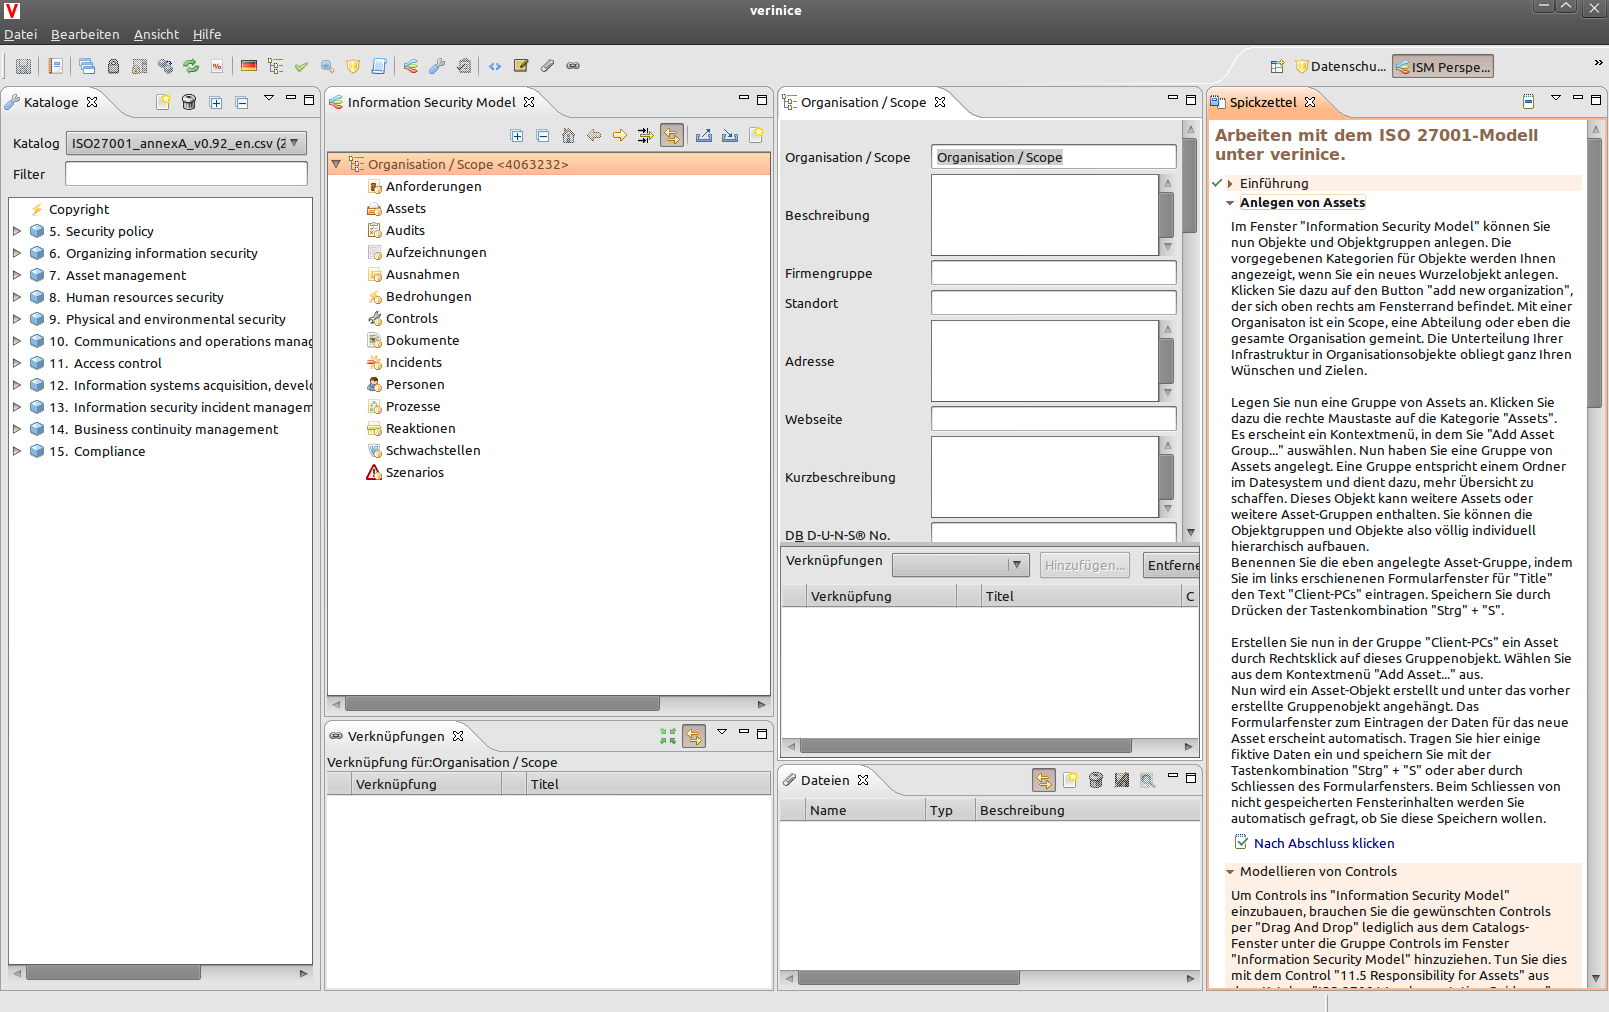
\includegraphics[scale=.21]{Screenshot/ISM-Perspektive.png}
  \caption{Standardkonfiguration von \textit{verinice} am Beispiel der
    ISM-Perspektive}
  \label{fig:standardkonfiguration-von-verinice}
\end{figure}


\subsection{Lizenzierung}

\textit{verinice} ist freie Software, die unter der \textit{GNU General Public
License, Version 3 (GPLv3)} veröffentlicht
wird.\footnote{\url{http://www.gnu.org/licenses/gpl-3.0.txt}} Verwendete
Komponenten stehen \ua unter der {\em Apache
License}\footnote{\url{http://www.apache.org/licenses/LICENSE-2.0}} und der {\em
Eclipse Public License}\footnote{\url{http://opensource.org/licenses/EPL-1.0}}.
Über das Hilfe-Menü erhalten Sie eine Übersicht über die Lizenzen der einzelnen
Plugins. Diese sind in \textit{verinice} unter $\textit{Hilfe}\to\textit{Info
über verinice}$ zu finden.


\subsection{Deinstallation}

Zur Deinstallation entfernen Sie einfach den Ordner, in welchen
\textit{verinice} extrahiert wurde sowie das von \textit{verinice} angelegte
Arbeitsverzeichnis \texttt{verinice} aus dem Benutzerverzeichnis.


\section{Installation des Servers für den Betrieb von \textit{verinice.PRO}}

Die benötigten Installationsanleitungen können Sie im Download-Bereich für
\textit{verinice.PRO}-Kunden\footnote{\url{https://update.verinice.com/pub/Manuals/}}
herunterladen. Dafür benötigen Sie die entsprechenden Zugangsdaten, die Sie im
Rahmen einer Subskription für \textit{verinice.PRO} erhalten.


\chapter{Symbole und Tastenkombinationen}

\section{Grundsymbole}
Die Grundsymbole teilen sich in vier verschiedene Gruppen:
\newline\\
\textbf{Allgemeine Symbole}
%\renewcommand{\arraystretch}{1.2}

\begin{longtable}{| c | p{0.7\textwidth} |}
\hline
\raisebox{-0.6\height}{\textbf{Symbol}} & \raisebox{-0.6\height}{\textbf{Bedeutung}} \\[10pt]
\hline\hline
\raisebox{-0.6\height}{
\includegraphics{Icon/New_persp.png}} & \raisebox{-0.6\height}{{Perspektiven-Auswahl}} \\[10pt] \hline
\raisebox{-0.6\height}{
\includegraphics{Icon/Disk.png}} & \raisebox{-0.6\height}{Speichern} \\[10pt] \hline
\raisebox{-0.6\height}{
\includegraphics{Icon/Report.png}} & \raisebox{-0.6\height}{Report erzeugen} \\[10pt] \hline
\raisebox{-0.6\height}{
\includegraphics{Icon/Masseneditor.png}} & \raisebox{-0.6\height}{Gleichartige Elemente gemeinsam editieren} \\[10pt] \hline
\raisebox{-0.6\height}{
\includegraphics{Icon/Zugriffsrechte.png}} & \raisebox{-0.6\height}{Zugriffsrechte bearbeiten} \\[10pt] \hline
\raisebox{-0.6\height}{
\includegraphics{Icon/Berechtigungsprofile.png}} & \raisebox{-0.6\height}{Berechtigungsprofile bearbeiten} \\[10pt] \hline
\raisebox{-0.6\height}{
\includegraphics{Icon/user_suit.png}} & \raisebox{-0.6\height}{Accounts bearbeiten} \\[10pt] \hline
\raisebox{-0.6\height}{
\includegraphics{Icon/user_add.png}} & \raisebox{-0.6\height}{Account hinzufügen} \\[10pt] \hline
\raisebox{-0.6\height}{
\includegraphics{Icon/user_disabled.png}} & \raisebox{-0.6\height}{Account deaktivieren} \\[10pt] \hline
\raisebox{-0.6\height}{
\includegraphics{Icon/group.png}} & \raisebox{-0.6\height}{Account-Gruppen} \\[10pt] \hline
\raisebox{-0.6\height}{
\includegraphics{Icon/group_add.png}} & \raisebox{-0.6\height}{Account-Gruppe hinzufügen} \\[10pt] \hline
\raisebox{-0.6\height}{
\includegraphics{Icon/group_edit.png}} & \raisebox{-0.6\height}{Account-Gruppe bearbeiten} \\[10pt] \hline
\raisebox{-0.6\height}{
\includegraphics{Icon/group_delete.png}} & \raisebox{-0.6\height}{Account-Gruppe löschen} \\[10pt] \hline
\raisebox{-0.6\height}{
\includegraphics{Icon/folder_table.png}} & \raisebox{-0.6\height}{Report-Ablage} \\[10pt] \hline
\raisebox{-0.6\height}{
\includegraphics{Icon/Aktualisieren.png}} & \raisebox{-0.6\height}{View neu laden} \\[10pt] \hline
\raisebox{-0.6\height}{
\includegraphics{Icon/Verinice_linked.png}} & \raisebox{-0.6\height}{Verknüpfe mit Editor} \\[10pt] \hline
\raisebox{-0.6\height}{
\includegraphics{Icon/Baustein.png}} & \raisebox{-0.6\height}{Baustein / Control-Gruppe (je nach Perspektive)} \\[10pt] \hline
\raisebox{-0.6\height}{
\includegraphics{Icon/Massnahmenbrowser.png}} & \raisebox{-0.6\height}{Objektbrowser} \\[10pt] \hline
\raisebox{-0.7\height}{
\includegraphics{Icon/Notizen.png}} & \raisebox{-0.7\height}{Notizen} \\[10pt] \hline
\raisebox{-0.6\height}{
\includegraphics{Icon/Hinzufuegen.png}} & \raisebox{-0.6\height}{Dateien} \\[10pt] \hline
\raisebox{-0.6\height}{
\includegraphics{Icon/Relationen.png}} & \raisebox{-0.6\height}{Relationen} \\[10pt] \hline
\raisebox{-0.6\height}{
\includegraphics{Icon/quickfix_warning_obj.png}} & \raisebox{-0.6\height}{Validierung} \\[10pt] \hline
\raisebox{-0.6\height}{
\includegraphics{Icon/Unbearbeitet.png}} & \raisebox{-0.6\height}{Umsetzungsstatus {\em Unbearbeitet}} \\[10pt] \hline
\raisebox{-0.6\height}{
\includegraphics{Icon/Nein.png}} & \raisebox{-0.6\height}{Umsetzungsstatus {\em Nein}} \\[10pt] \hline
\raisebox{-0.6\height}{
\includegraphics{Icon/Teilweise.png}} & \raisebox{-0.6\height}{Umsetzungsstatus {\em Teilweise}} \\[10pt] \hline
\raisebox{-0.6\height}{
\includegraphics{Icon/Okay.png}} & \raisebox{-0.6\height}{Umsetzungsstatus {\em Ja}} \\[10pt] \hline
\raisebox{-0.6\height}{
\includegraphics{Icon/Entbehrlich.png}} & \raisebox{-0.6\height}{Umsetzungsstatus {\em Entbehrlich}} \\[10pt] \hline
\raisebox{-0.6\height}{
\includegraphics[scale=5]{Icon/Alien.png}} & \raisebox{-0.6\height}{Importierte und nicht integrierte Zielobjekte} \\[10pt] \hline
\raisebox{-1\height}{
\includegraphics{Icon/Oeffnen.png}} & \raisebox{-0.6\height}{\parbox{0.7\textwidth}{Katalog importieren / Neue Organisation hinzufügen \linebreak / Datei hinzufügen}} \\[10pt] \hline
\raisebox{-0.6\height}{
\includegraphics{Icon/Verknuepfungen.png}} & \raisebox{-0.6\height}{Verknüpfen mit Zielobjekten} \\[10pt] \hline
\raisebox{-3.0\height}{$\leftarrow$ $\rightarrow$ $\downarrow$ $\uparrow$} & einer der vier Pfeile ersetzt das vorherige Symbol und gibt in Verbindung
mit dem dunklen Rahmen den neuen Platz der Sicht an, sobald Sie mit gedrückter linker Maustaste die aktuelle Sicht verlassen \\[10pt] \hline
\raisebox{-1.0\height}{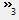
\includegraphics{Icon/Versteckte_Reiter.png}} & wenn nicht alle geöffneten Reiter in einer Sicht angezeigt werden können, erscheint
dieses Symbol; die Zahl hinter dem Doppelpfeil zeigt die Anzahl der versteckten Reiter  \\[10pt] \hline
\raisebox{-1\height}{
\includegraphics{Icon/Filter.png}} & Filter-Einstellungen zum selektieren von einzelnen Elementen, nach denen gesucht werden soll \\[10pt] \hline
\raisebox{-0.6\height}{
\includegraphics{Icon/Siegelstufe_A.png}} \raisebox{-0.6\height}{
\includegraphics{Icon/Siegelstufe_B.png}} \raisebox{-0.6\height}{
\includegraphics{Icon/Siegelstufe_C.png}} \raisebox{-0.6\height}{
\includegraphics{Icon/Siegelstufe_Z.png}} & \raisebox{-0.6\height}{Siegelstufen von Maßnahmen (A, B, C, Z)} \\[10pt] \hline
\raisebox{-0.6\height}{
\includegraphics{Icon/Gefaehrdungen.png}} & \raisebox{-0.6\height}{Gefährdungen} \\[10pt] \hline
\raisebox{-1\height}{
\includegraphics{Icon/Ziel.png}} & innerhalb der Sicht Relationen springen Sie hiermit zum Ziel der markierten Verknüpfung \\[10pt] \hline
\raisebox{-1.5\height}{
\includegraphics{Icon/Haengt_Ab.png}} & {\em hängt ab von} (tiefer stehendes Zielobjekt im IT-Verbund / Organisation wurden mit einer höher stehenden Komponente verknüpft) \\[10pt] \hline
\raisebox{-1.5\height}{
\includegraphics{Icon/Noetig_Fuer.png}} & {\em ist nötig für} (höher stehende Komponente im IT-Verbund / Organisation wurde einem tiefer stehenden Zielobjekt verknüpft) \\[10pt] \hline
\raisebox{-0.6\height}{
\includegraphics{Icon/Verknuepfung_Aufheben.png}} & \raisebox{-0.6\height}{Verknüpfung aufheben} \\[10pt] \hline
\raisebox{-0.6\height}{
\includegraphics{Icon/Export.png}} & {Export einer oder mehrerer Organisationen, IT-Verbünden oder Security-Assessments} \\[10pt] \hline
\raisebox{-0.6\height}{
\includegraphics{Icon/Import.png}} & {Import einer oder mehrerer Organisationen, IT-Verbünden oder Security-Assessments} \\[10pt] \hline
\raisebox{-0.6\height}{
\includegraphics{Icon/Nav_home.png}} & \raisebox{-0.6\height}{zurück zum Wurzelobjekt} \\[10pt] \hline
\raisebox{-0.6\height}{
\includegraphics{Icon/Cheatsheet_view.png}} & \raisebox{-0.6\height}{Spickzettel} \\[10pt] \hline
\raisebox{-0.6\height}{
\includegraphics{Icon/Forward_nav.png}} & \raisebox{-0.6\height}{In ein Gruppenzielobjekt gelangen} \\[10pt] \hline
\raisebox{-0.6\height}{
\includegraphics{Icon/Backward_nav.png}} & \raisebox{-0.6\height}{Aus einem Gruppenzielobjekt gelangen} \\[10pt] \hline
\raisebox{-0.6\height}{\includegraphics{Icon/Edit.png}} & \raisebox{-0.6\height}{Editiere} \\[10pt] \hline
\raisebox{-0.6\height}{\includegraphics{Icon/Delete.png}} & \raisebox{-0.6\height}{Löschen} \\[10pt] \hline
\raisebox{-0.6\height}{\includegraphics[scale=0.15]{Icon/Save.png}} & \raisebox{-0.6\height}{Datei speichern} \\[10pt] \hline
\raisebox{-0.6\height}{\includegraphics[scale=0.2]{Icon/Suchen.png}} & \raisebox{-0.6\height}{Datei öffnen} \\[10pt] \hline
\raisebox{-0.6\height}{\includegraphics[scale=0.7]{Icon/search.png}} & \raisebox{-0.6\height}{verinice-Suche} \\[10pt] \hline
\caption{Allgemeine Symbole}
\end{longtable}
\newpage
\textbf{Symbole für die Perspektiven}
\begin{longtable}{| c | p{0.8\textwidth} |}
    \hline
    \textbf{Symbol}                                                         & \textbf{Bedeutung} \\[10pt]
    \hline\hline
    \raisebox{-0.6\height}{\includegraphics[scale=0.6]{Icon/gs.png}}        & BSI Grundschutz Perspektive \\[10pt] \hline
    \raisebox{-0.6\height}{\includegraphics[scale=0.6]{Icon/greenbone.png}} & Greenbone Perspektive \\[10pt] \hline
    \raisebox{-0.6\height}{\includegraphics[scale=0.6]{Icon/ism.png}}       & ISM Perspektive \\[10pt] \hline
    \raisebox{-0.6\height}{\includegraphics[scale=0.6]{Icon/bp.png}}        & Modernisierter BSI Grundschutz Perspektive \\[10pt] \hline
    \raisebox{-0.6\height}{\includegraphics[scale=0.6]{Icon/vda.png}}       & Security Assessment Perspektive \\[10pt] \hline
    \caption{Perspektiven-Symbole}
\end{longtable}
\textbf{Symbole in der IT-Grundschutz-Perspektive}
\begin{longtable}{| c | p{0.8\textwidth} |}
\hline
\textbf{Symbol} & \textbf{Bedeutung} \\[10pt]
\hline\hline
\raisebox{-0.6\height}{\includegraphics{Icon/GS_Kataloge.png}} & GS-Kataloge \\[10pt] \hline
\raisebox{-0.6\height}{\includegraphics{Icon/GS_Modell.png}} & Grundschutz-Modell \\[10pt] \hline
\raisebox{-0.6\height}{\includegraphics{Icon/Okay.png}} & Realisierungsplan \\[10pt] \hline
\raisebox{-0.7\height}{\includegraphics{Icon/page_find.png}} & Prüfplan \\[10pt] \hline
\raisebox{-0.6\height}{\includegraphics{Icon/Datenschutz.png}} & Datenschutz \\[10pt] \hline
\raisebox{-0.6\height}{\includegraphics{Icon/Richtlinien.png}} & Externe Links \\[10pt] \hline
\raisebox{-0.6\height}{\includegraphics{Icon/Mitarbeiter.png}} & Mitarbeiter \\[10pt] \hline
\raisebox{-0.6\height}{\includegraphics{Icon/Anwendung.png}} & Anwendungen \\[10pt] \hline
\raisebox{-0.6\height}{\includegraphics{Icon/Raeume.png}} & Räume \\[10pt] \hline
\raisebox{-0.6\height}{\includegraphics{Icon/Clients.png}} & Clients  \\[10pt] \hline
\raisebox{-0.6\height}{\includegraphics{Icon/Tk_komponenten.png}} & TK-Komponenten \\[10pt] \hline
\raisebox{-0.6\height}{\includegraphics{Icon/Gebaeude.png}} & Gebäude \\[10pt] \hline
\raisebox{-0.6\height}{\includegraphics{Icon/Server.png}} & Server \\[10pt] \hline
\raisebox{-0.6\height}{\includegraphics{Icon/Sonstige.png}} & Sonstige \\[10pt] \hline
\raisebox{-0.6\height}{\includegraphics{Icon/Netzwerkverbindungen.png}} & Netzwerkverbindungen \\[10pt] \hline
\raisebox{-0.6\height}{\includegraphics{Icon/Risikoanalyse.png}} & Risikoanalyse \\[10pt] \hline
\raisebox{-1\height}{\includegraphics{Icon/Konsolidator.png}} & Gleiche Bausteine und ihre Maßnahmen konsolidieren \\[10pt] \hline
\caption{Symbole in der IT-Grundschutz-Perspektive}
\end{longtable}
\textbf{Symbole in der ISM-Perspektive}
\begin{longtable}{| c | p{0.8\textwidth} |}
\hline
\textbf{Symbol} & \textbf{Bedeutung} \\[10pt]
\hline\hline
\raisebox{-0.7\height}{\includegraphics{Icon/Informationssicherheitsmodell.png}} & Informationssicherheitsmodell \\[10pt] \hline
\raisebox{-0.6\height}{\includegraphics{Icon/16-paper-calculate-percent.png}} & Risikoanalyse durchführen \\[10pt] \hline
\raisebox{-0.6\height}{\includegraphics{Icon/Tasks.png}} & Aufgaben bearbeiten \\[10pt] \hline
\raisebox{-0.6\height}{\includegraphics{Icon/Chart_pie.png}} & Information-Security-Assessment-Fortschritt \\[10pt] \hline
\raisebox{-0.6\height}{\includegraphics{Icon/16-paper-gavel-alt.png}} & Anforderungen \\[10pt] \hline
\raisebox{-0.6\height}{\includegraphics{Icon/Asset.png}} & Assets \\[10pt] \hline
\raisebox{-0.6\height}{\includegraphics{Icon/Clipboard_comment.png}} & Audit: Befragungen \\[10pt] \hline
\raisebox{-0.6\height}{\includegraphics{Icon/Clipboard_report.png}} & Audit: Findings \\[10pt] \hline
\raisebox{-0.6\height}{\includegraphics{Icon/Clipboard_eye.png}} & Audit: Nachweise \\[10pt] \hline
\raisebox{-0.6\height}{\includegraphics{Icon/Clipboard_audit.png}} & Audits \\[10pt] \hline
\raisebox{-0.6\height}{\includegraphics[scale=0.3]{Icon/Text.png}} & Aufzeichnungen \\[10pt] \hline
\raisebox{-0.6\height}{\includegraphics{Icon/16-paper-excerpt-yellow.png}} & Ausnahmen \\[10pt] \hline
\raisebox{-0.6\height}{\includegraphics{Icon/Lightening.png}} & Bedrohungen \\[10pt] \hline
\raisebox{-0.6\height}{\includegraphics{Icon/Controls.png}} & Controls \\[10pt] \hline
\raisebox{-0.6\height}{\includegraphics{Icon/Document.png}} & Dokumente \\[10pt] \hline
\raisebox{-0.6\height}{\includegraphics{Icon/Incident.png}} & Incidents \\[10pt] \hline
\raisebox{-0.6\height}{\includegraphics{Icon/Mitarbeiter.png}} & Personen \\[10pt] \hline
\raisebox{-0.6\height}{\includegraphics{Icon/Prozesse.png}} & Prozesse \\[10pt] \hline
\raisebox{-0.6\height}{\includegraphics{Icon/Reaktionen.png}} & Reaktionen \\[10pt] \hline
\raisebox{-0.6\height}{\includegraphics{Icon/Schwachstellen.png}} & Schwachstellen \\[10pt] \hline
\raisebox{-0.6\height}{\includegraphics{Icon/Szenarios.png}} & Szenarios \\[10pt] \hline
\raisebox{-0.6\height}{\includegraphics{Icon/Folder_decorator.png}} & Kennzeichnung für Gruppenzielobjekte \\[10pt] \hline
\raisebox{-0.6\height}{\includegraphics{Icon/Verinice_derive.png}} & Status ableiten \\[10pt] \hline
\raisebox{-0.6\height}{\includegraphics{Icon/Expandall.png}} & Alle Wurzelobjekte aufklappen \\[10pt] \hline
\raisebox{-0.6\height}{\includegraphics{Icon/Collapseall.png}} & Alle Wurzelobjekte zuklappen \\[10pt] \hline
\caption{Symbole in der ISM-Perspektive}
\end{longtable}
Die Symbole der Perspektive Security Assessment entsprechen denen der ISM-Perspektive.

\textbf{Symbole in der Perspektive Modernisierter IT-Grundschutz}
\begin{longtable}{| c | p{0.8\textwidth} |}
    \hline
    \textbf{Symbol}                                                        & \textbf{Bedeutung} \\[10pt]
    \hline\hline
    \raisebox{-0.6\height}{\includegraphics{Icon/bp_catalog.png}}          & IT-Grundschutz-Kompendium \\[10pt] \hline
    \raisebox{-0.6\height}{\includegraphics{Icon/bp.png}}                  & Modernisierter BSI Grundschutz \\[10pt] \hline
    \raisebox{-0.6\height}{\includegraphics{Icon/bp_business_process.png}} & Geschäftsprozesse \\[10pt] \hline
    \raisebox{-0.6\height}{\includegraphics{Icon/bp_application}}          & Anwendungen \\[10pt] \hline
    \raisebox{-0.6\height}{\includegraphics{Icon/bp_it_system.png}}        & IT-Systeme \\[10pt] \hline
    \raisebox{-0.6\height}{\includegraphics{Icon/bp_ics_system.png}}       & ICS-Systeme \\[10pt] \hline
    \raisebox{-0.6\height}{\includegraphics{Icon/bp_device.png}}           & Andere/IOT-Systeme \\[10pt] \hline
    \raisebox{-0.6\height}{\includegraphics{Icon/bp_network.png}}          & Kommunikationsverbindungen \\[10pt] \hline
    \raisebox{-0.6\height}{\includegraphics{Icon/bp_room.png}}             & Räume \\[10pt] \hline
    \raisebox{-0.6\height}{\includegraphics{Icon/bp_person.png}}           & Personen \\[10pt] \hline
    \raisebox{-0.6\height}{\includegraphics{Icon/bp_requirement.png}}      & Bausteine \\[10pt] \hline
    \raisebox{-0.6\height}{\includegraphics{Icon/bp_threat.png}}           & Gefährdungen \\[10pt] \hline
    \raisebox{-0.6\height}{\includegraphics{Icon/bp_safeguard.png}}        & Maßnahmen \\[10pt] \hline
    \caption{Symbole in der Perspektive Modernisierter IT-Grundschutz}
\end{longtable}

Alle Grundsymbole innerhalb des Informationssicherheitsmodells und des Grundschutzmodells können individuell geändert werden.
Klicken Sie dazu das entsprechende Symbol (Mehrfachselektion ist möglich) in der Baumstruktur mit der rechten Maustaste an und wählen Sie die Option
\textbf{Ändere Icon...} im Kontextmenü. Im darauffolgenden Dialogfenster können die Icons nach Kategorien gefiltert,
anschließend mit der linken Maustaste ausgewählt und mit dem \textbf{OK}-Button bestätigt werden.
Um ein Standard-Icon für ein ausgewähltes Objekt oder mehrere Objekte wieder herzustellen, sollten Sie die Objekte markieren,
die Option \textbf{Ändere Icon...} im Kontextmenü erneut aufrufen, die Checkbox für \textbf{Zeige Standard-Icon} aktivieren und
die Auswahl mit dem \textbf{OK}-Button bestätigen. Damit erhält das entsprechende Objekt (bzw. mehrere Objekte) das Grundsymbol.
Die Änderungen für Icons können nur innerhalb des Modell-Views für Zielobjekte vorgenommen werden.

\section{Tastenbelegung}
Nachfolgend finden Sie eine Liste aller Tastaturkürzel, die Ihnen das Arbeiten unter verinice erleichtern können:
\\
\begin{longtable}{| p{0.4\textwidth} | p{0.5\textwidth} |}
\hline
\textbf{Funktion} & \textbf{Tastenbelegung} \\[10pt]
\hline\hline
Aktive Sicht maximieren & \textbf{Strg} + \textbf{M} \\[10pt] \hline
Alle speichern (Alle Änderungen für Zielobjekte speichern) & \textbf{Strg} + \textbf{Umschalttaste} + \textbf{S} \\[10pt] \hline
Alle auswählen (Alle Zielobjekte auswählen) & \textbf{Strg} + \textbf{A} \\[10pt] \hline
Alle schließen (Alle offenen Editoren schließen) & \textbf{Strg} + \textbf{Umschalttaste} + \textbf{W} \\[10pt] \hline
Ausschneiden (Ausschneiden von Zielobjekten) & \textbf{Strg} + \textbf{X} \\[10pt] \hline
Beenden (verinice beenden) & \textbf{Strg} + \textbf{Umschalttaste} + \textbf{X} \\[10pt] \hline
Beitragendes Plugin zeigen & \textbf{Umschalttaste} + \textbf{Alt} + \textbf{F3} \\[10pt] \hline
Benutzerrechte anzeigen & \textbf{Strg} + \textbf{R} (diese Funktion ist ausschließlich bei Anbindung an einen verinice.\textsc{PRO}-Server verfügbar) \\[10pt] \hline
Editor aktivieren & \textbf{F12} \\[10pt] \hline
Eigenschaften anzeigen & \textbf{Alt} + \textbf{Eingabetaste} \\[10pt] \hline
Einfügen & \textbf{Strg} + \textbf{V} \\[10pt] \hline
Liste der Tastenkürzel von verinice anzeigen & \textbf{Strg} + \textbf{Umschalttaste} + \textbf{L} \\[10pt] \hline
Kopieren & \textbf{Strg} + \textbf{C} \\[10pt] \hline
Kopieren mit Verknüpfungen & \textbf{Strg} + \textbf{Umschalttaste} + \textbf{C} \\[10pt] \hline
Perspektivenumschaltmenü & \textbf{Strg} + \textbf{F8} \\[10pt] \hline
Gesamtes verinice-Fenster verschieben & \textbf{Alt} + \textbf{F7} \\[10pt] \hline
Viewumschaltmenü (Umschalten zwischen Views) & \textbf{Strg} + \textbf{F7} \\[10pt] \hline
Editorumschaltmenü (Umschalten zwischen geöffneten Editoren) & \textbf{Strg} + \textbf{F6} \\[10pt] \hline
Schließen & \textbf{Strg} + \textbf{W} \\[10pt] \hline
Objekt oder Objektgruppe löschen & \textbf{Entf} \\[10pt] \hline
Speichern & \textbf{Strg} + \textbf{S} \\[10pt] \hline
Neues Objekt & \textbf{Strg} + \textbf{N} (ausschließlich in der ISM-Perspektive) \\[10pt] \hline
Neue Objektgruppe & \textbf{Strg} + \textbf{Umschalttaste} + \textbf{N} (ausschließlich in der ISM-Perspektive) \\[10pt] \hline
Kontextmenü des aktiven Views aufrufen & \textbf{Alt} + \textbf{-} \\[10pt] \hline
Alle editieren (Aufruf des Masseneditors) & \textbf{Strg} + \textbf{Umschalttaste} + \textbf{B} \\[10pt] \hline
Zeige Vorschläge für Bausteine & \textbf{Strg} + \textbf{O} (ausschließlich in der Grundschutz-Perspektive)  \\[10pt] \hline
Editor-Auswahl-Menü aufrufen & \textbf{Umschalttaste} + \textbf{Strg} + \textbf{E} \\[10pt] \hline
Alle Views in verinice aktualisieren & \textbf{Strg} + \textbf{F5} \\[10pt] \hline
\caption{Tastenbelegung}
\end{longtable}
Eine Übersichtsliste der Tastaturkürzel lässt sich auch über das Menü
\textbf{Hilfe \textgreater Hilfe für Tastenbelegung} aufrufen.

\section{Verwendung verschiedener Perspektiven} \label{Verwendung verschiedener Perspektiven}
In verinice können Sie zwischen unterschiedlichen Perspektiven wählen. Diese wurden eingeführt, um unterschiedliche Standards besser
abzubilden. Bei der Auswahl einer bestimmten Perspektive werden automatisch die passenden Sichten (Fenster/Views) angezeigt.
\newline \\
Sie können die Perspektive über das Menü
\newline\mbox{\textbf{Ansicht \textgreater Zeige Perspektive... \textgreater \textless gewünschte Perspektive\textgreater}} umschalten.
\newline \\
Alternativ können Sie auch die Schaltflächen zum Öffnen der einzelnen Perspektiven (am oberen rechten Fensterrand) verwenden,
vlg.\ Abbildung~\ref{fig:window_persp}.

\begin{figure}[htb!]
  \centering
  \includegraphics[width=0.5\textwidth]{Screenshot/persp}
  \caption{Schaltflächen verschiedener Perspektiven}
  \label{fig:window_persp}
\end{figure}

\subsection{BSI-IT-Grundschutz-Perspektive}
Die Perspektive {\em BSI Grundschutz} unterstützt bei der Erstellung und Aufrechterhaltung eines ISMS gemäß der IT-Grundschutz-Vorgehensweise
und den BSI-Standards 100-1, 100-2, 100-3 und 100-4. Eine ausführliche Beschreibung zum Arbeiten
in dieser Perspektive finden Sie im
Hauptabschnitt {\em \ref{Arbeiten in der Grundschutz-Perspektive} \nameref{Arbeiten in der Grundschutz-Perspektive}}.

\subsection{Perspektive Modernisierter Grundschutz}
Die Perspektive für den modernisierten BSI Grundschutz unterstützt bei der
Erstellung und Aufrechterhaltung eines ISMS gemäß der
IT-Grundschutz-Vorgehensweise und den BSI-Standards 200-1, 200-2, 200-3 sowie
zukünftig 200-4. Eine ausführliche Beschreibung zum Arbeiten in dieser
Perspektive finden Sie im Hauptabschnitt \emph{\ref{chap:baseline-protection} \nameref{chap:baseline-protection}}.

\subsection{ISM-Perspektive}
Die {\em ISM Perspektive} ist für die Umsetzung der Standard-Reihe ISO 2700x ausgelegt. Als generische Perspektive kann sie aber auch zum
allgemeinen Risiko-Management oder zur Umsetzung organisationsinterner Vorgaben verwendet werden. Eine ausführliche Beschreibung zum
Arbeiten in dieser Perspektive finden Sie im Hauptabschnitt {\em \ref{Arbeiten in der ISM-Perspektive} \nameref{Arbeiten in der ISM-Perspektive}}.

\section{Das Sichten-Prinzip}
Die einzelnen Bildschirmbereiche (Fenster) heißen {\em Ansichten} oder {\em Views} (siehe Abb. \ref{Standardansicht in der ISM-Perspektive}).
\newline\\
Grundsätzlich kann jeder einzelne View verschoben, in Höhe und Breite geändert (teilweise auch in andere Fenster platziert) und über die
entsprechenden Reiter aktiviert werden. Weiterhin können Sie eine vertikale, horizontale oder gemischte Anordnung der einzelnen Sichten
vornehmen. Es ist möglich, Views komplett aus dem verinice-Applikationsfenster als eigenständiges Fenster herauszulösen (Drag\&Drop des Views).
Die Sichten können vom Benutzer individuell angeordnet werden. Durch das
Klicken mit der rechten Maustaste auf das obere Titelfeld einer Sicht wird jeweils das Kontextmenü geöffnet. Damit haben Sie zusätzlich
eine Fülle von weiteren Bearbeitungsoptionen zur Auswahl.
\newline\\
Bei der Minimierung oder Maximierung von Views kann es zu einer automatischen Verschiebung von anderen geöffneten Fenstern
oder zur Aktivierung der Schnellansicht führen.
\begin{figure}[htb!]
  \centering
  \includegraphics[scale=.43]{Screenshot/800px-Sichten-Prinzip.jpg}
  \caption{\label{Standardansicht in der ISM-Perspektive} Standardansicht in der ISM-Perspektive}
\end{figure}
Jede offene Sicht wird bei Bedarf aktualisiert. Durch die offenen Perspektiven und Views können Sie mit \textbf{Strg+F8} für Perspektiven und mit \textbf{Strg+F7} für Views wechseln.
Eine Aktualisierung lässt sich gegebenenfalls mit dem Button \icon{Icon/Aktualisieren.png} forcieren, um z.B. das Modell der Infrastruktur in ihrer Darstellung zu aktualisieren.
\newline\\
Einzelne Views weisen den Button \icon{Icon/Verinice_linked.png} \textbf{Verknüpfe mit Editor} auf.
Das Aktivieren dieser Funktion sorgt dafür, dass in dem entsprechenden View immer die Informationen des ausgewählten Editors
angezeigt werden. Das ist besonders beim gleichzeitigen Arbeiten mit mehreren offenen Editoren hilfreich. Die Funktion kann in
den betroffenen Views jeweils ein- oder ausgeschaltet werden. Sollten Sie beispielsweise mehrere Editoren geöffnet haben und
schalten zwischen diesen per Tab hin und her, so werden die dazugehörigen Objekte im Modell-View automatisch selektiert und
ggf. die Informationen im Objektbrowser aktualisiert.
\newline\\
Wenn Sie die Funktion deaktivieren, so erfolgt keine automatische Aktualisierung der Informationen in dem View.

\section{Benutzung der Editoren}
Im Editor werden zum einem Informationen und Werte zu bestimmten Objektattributen zugewiesen und zum anderen Relationen zwischen Zielobjekten erstellt.
Editoren werden dann eingeblendet, wenn Sie ein beliebiges Zielobjekt im Objektbaum doppelt anklicken.

\chapter{Basisfunktionen}
\section{Abbrechen}
In vielen Situationen lassen sich die Eingaben oder Menüfenster abbrechen, so dass die Änderungen oder Eingaben seit dem
letzten Aufruf der Fenster oder Menüs unwirksam bleiben. Klicken Sie dazu den Button \textbf{Abbrechen}.

\section{Speichern}
Diese Funktion sichert die Eingaben des Benutzers in einem Eingabeformular und wird aktiviert durch das Betätigen von \icon{Icon/Disk.png}
(alternativ durch die Tastenkombination: \textbf{Strg+S}). Beim Schließen eines
Editors nach vorheriger Dateneingabe oder \mbox{-veränderung} werden Sie in einem Popup-Menü gefragt, ob die Änderungen gespeichert werden sollen.

\section{Reports erzeugen} \label{Reports erzeugen}
Daten aus verinice können als Reports in unterschiedlichen Formaten ausgegeben werden. Häufig werden die Reports als
Statusinformation und Entscheidungshilfe für die Leitungsebene oder Auditberichte verwendet. Über das Symbol \icon{Icon/Report.png}
(oder alternativ über das Menü: \textbf{Datei \textgreater  Report erstellen...}) können Sie die Ausgabe von Reports konfigurieren. Um einen Report
für einen bestimmten Geltungsbereich zu erzeugen, können Sie auch mit der rechten Maustaste auf das oberste Wurzelobjekt
klicken und die Option \textbf{Erzeuge Report...} auswählen. Damit wird die Auswahl des Geltungsbereichs ausschließlich auf das selektierte Wurzelobjekt
eingeschränkt.\\ Manche Reports unterstützen mehrere Wurzelobjekte. Bei diesen
Reports haben Sie die Möglichkeit den Report über alle verfügbaren
Geltungsbereiche auszuführen. Für eine spezifische Auswahl markieren Sie die
gewünschten Wurzelobjekte (mit \textbf{Strg+Klick}), klicken Sie mit der rechten
Maustaste auf eines der selektierten Objekte und wählen Sie \textbf{Erzeuge
Report...} Der Geltungsbereich umfasst nun die selektierten Objekte.
Allerdings kann diese Auswahl im Dialog nicht mehr nachträglich angepasst
werden.\\

Im ersten Schritt gilt es eine Vorlage für den zu erzeugenden Report
auszuwählen. Alle Vorlagen, die in verinice enthalten sind, finden Sie
im Drop-Down-Menü \textbf{Report auswählen: Report aus Vorlage...}.
Sollen eigene Report-Templates in dieser Auswahlbox verfügbar sein,
können Sie diese auf der Dateisystemebene einfügen (siehe Kapitel \ref{sec:reports-hinzufuegen})
oder die wesentliche komfortablere Reportablage von verinice.PRO nutzen (siehe Kapitel \ref{reportdeposit} \nameref{reportdeposit}).

Selektieren Sie anschließend den Geltungsbereich für den der Report erzeugt werden soll
(typischerweise der Audit- oder Organisationsname, den Sie im Wurzelelement ausgewählt haben). Im nächsten Schritt müssen Sie noch das Ausgabeformat
und den Ablageort der Report-Datei auswählen. Wenn die Checkbox \textbf{immer dieses Verzeichnis benutzen} ausgewählt ist merkt sich verinice die Verzeichnisse für die Report-Vorlage bzw. Ausgabedatei und öffnet den entsprechenden Ordner bei der nächsten Report-Generierung wieder.
\newline\\
Für die Ausgabe von Reports stehen Ihnen (so die Konfigurationsdatei des Templates (siehe oben) nicht angepasst wurde) folgende Formate zur Verfügung:
\begin{itemize}
 \item \textsc{PDF}
 \item \textsc{HTML}
 \item \textsc{XLS}
 \item \textsc{DOC}
 \item \textsc{ODT}
 \item \textsc{ODS}
\end{itemize}
Optional steht Ihnen die Funktion \textbf{Reportcache zurücksetzen} zur
Verfügung. Die Betätigung dieses Buttons löst ein Zurücksetzen eines
internen Speichers (Cache) aus,
der die bei der Reportgenerierung erzeugten Zwischenergebnisse zur
Wiederverwendung vorhält. Dies hat zur Folge, dass bei Generierung von
mehreren Reports in Reihe nicht jede abzubildende Information aus der Datenbank geladen und berechnet werden muss, sondern unter Umständen bereits im
Zwischenspeicher vorliegt, das beschleunigt die Generierung des Reports. Ist seit
dem letzten Report allerdings der Datenbestand verändert worden, so ist
es notwendig den Reportcache zu leeren um eine Abbildung der aktuellen
Daten zu garantieren.
\newline\\
Durch Klicken auf den OK-Button, werden Ihre Eingaben bestätigt und der Report erstellt (siehe Abb. \ref{Report erzeugen}).
\newline
Weitere Informationen zum Report-Cache finden Sie im Kapitel {\em \ref{Reports} \nameref{Reports}}.
\begin{figure}[htb!]
  \centering
  \includegraphics[scale=.45]{Screenshot/Reportdialog.png}
  \caption{\label{Report erzeugen} Report erzeugen}
\end{figure}
\newline\\
Wenn Sie Reports für die BSI-Grundschutz-Perspektive benötigen, lesen Sie im Unterkapitel {\em \ref {Reports erstellen} \nameref{Reports erstellen}} des Kapitels
{\em \ref{Arbeiten in der Grundschutz-Perspektive} \nameref{Arbeiten in der Grundschutz-Perspektive}}, welche Ausgaben möglich sind.
\newline\\
Wenn Sie Reports für die ISM-Perspektive benötigen, lesen Sie im Unterkapitel {\em \ref{ISM-Reports erstellen} \nameref{ISM-Reports erstellen}} des Kapitels
{\em \ref{Arbeiten in der ISM-Perspektive} \nameref{Arbeiten in der ISM-Perspektive}}, welche Ausgaben möglich sind.
\newline\\
Wenn Sie Reports für die VDA-Security-Assessment-Perspektive benötigen, lesen Sie im Unterkapitel {\em \ref{Report erstellen} \nameref{Report erstellen}} des
Kapitels {\em \ref{Arbeiten in der VDA-Perspektive} \nameref{Arbeiten in der VDA-Perspektive}}, welche Ausgaben möglich sind.

\section{Reports anpassen}
Die ausgelieferten Report-Vorlagen wurden mit \textbf{vDesigner}
erstellt, der unseren verinice.PRO-Kunden unter
\href{https://update.verinice.com}{update.verinice.com} zur Verfügung
steht.

Angepasste oder ganz individuelle zusätzliche Vorlagen für Reports
können auch bei SerNet in Auftrag gegeben werden.

\section{Reports hinzufügen}
\label{sec:reports-hinzufuegen}


Wenn Sie eine eigene Datei als Vorlage benutzen wollen, können Sie
diese in einem speziell dafür konfigurierbarem Verzeichnis
ablegen. Das Verzeichnis konfigurieren Sie über die Einstellung
\textbf{Bearbeiten \textgreater Einstellungen \textgreater Reports
  \textgreater Report Templates}. Die Standard-Einstellung ist das
Unterverzeichnis ``report\_templates\_local'' des Heimatverzeichnisses
(siehe {\em \ref{sec:installation} \nameref{sec:installation}}).  Wird
ein Reporttemplate im rptdesign-Dateiformat in diesem Verzeichnis
abgelegt, wird es in der Liste des Reportdialogs mit zur Auswahl
angeboten. Die dort zur Auswahl angebotenen Ausgabeformate und der
vorgeschlagene Name können über eine speziell für dieses Template
vorhandene Datei (dateiname.properties) konfiguriert werden. Diese
Datei wird, sofern nicht vorhanden, beim ersten Öffnen des
Reportdialogs angelegt und kann anschließend den eigenen Anforderungen
gemäß angepasst werden. Wird verinice nicht in der Standardsprache
(Englisch) ausgeführt, wird dem Dateinamen noch ein Länderkürzel
der Form ``dateiname\_de.properties'' eingefügt.\\

Benutzer von verinice.PRO können den Inhalt des Reportdialogs in der
Sicht \glqq Reportablage\grqq\ verwalten und damit auf alle
verinice-Client-Installationen verteilen. Diese Möglichkeit wird in
Kapitel {\em \ref{reportdeposit} \nameref{reportdeposit}} beschrieben.


\section{Gleichartige Elemente gemeinsam editieren}
Mit dem sogenannten \textbf{Masseneditor} können mehrere gleichartige Objekte zusammen bearbeitet werden. Markieren Sie dazu die zu
verändernden Objekte und betätigen anschließend \icon{Icon/Masseneditor.png} (alternativ: \textbf{Strg+Umschalttaste+B} oder über das
Menü \textbf{Bearbeiten \textgreater Alle editieren \textgreater Rechtsklick \textgreater Masseneditor}). So erscheint ein Popup-Fenster mit den Eingaben,
wie sie im Editor erscheinen würden. Tragen Sie hier alle gewünschten Daten ein. Alle abgespeicherten Veränderungen
werden dann auch für alle ausgewählten Objekte an gleicher Stelle übernommen. Felder, die Sie leer belassen, werden
nicht verändert (auch nicht, wenn sie vorher bereits befüllt waren).

\section{View neu laden}
Diese Funktion entspricht dem \textbf{Aktualisieren} und wird durch das Betätigen von \icon{Icon/Aktualisieren.png} (alternativ: Strg+F5) aktiviert.

\section{Verschieben und Kopieren von Objekten}
Für das Kopieren und Verschieben eines Objektes, wählen Sie das konkrete Objekt (im Modell-View) mit der rechten Maustaste aus. Daraufhin wählen Sie die gewünschte Funktion aus
dem Kontextmenü aus (\textbf{Kopieren} oder \textbf{Ausschneiden}) und verschieben das Objekt über die Funktion \textbf{Einfügen} an den Zielort.
Der Zielort sollte vorher durch Anklicken aktiviert werden.
\newline\\
Wenn Sie so ein Objekt kopieren, erzeugen Sie damit ein Objekt-Duplikat, was aber für die verinice-Applikation ein neues Objekt darstellt.
Alle Verknüpfungen des originären Objekts hat die Objekt-Kopie nicht mehr. Wenn Sie ein Objekt samt Verknüpfungen kopieren möchten, lesen Sie im
nachfolgenden Abschnitt nach, wie Sie dazu vorgehen müssen.
\newline\\
Beim Ausschneiden von Objekten bleiben alle Verknüpfungen erhalten.
\newline\\
\textbf{Achtung: Durch das Verwenden der Drag \& Drop-Funktion werden Objekte NICHT kopiert, sondern Verknüpfungen zwischen ihnen erzeugt.}
\newline\\
Beim Kopieren von Objekten werden die Lese- und Schreibrechte der Gruppe übernommen, in der die Kopie angelegt wurde. Beim Verschieben von Objekten bleiben die Lese- und Schreibrechte der verschobenen Objekte unverändert. Dieses Verhalten läßt sich in den Einstellungen ändern, so dass auch beim Verschieben die Lese- und Schreibrechte der Gruppe übernommen werden, in der die Objekte eingefügt wurden: \textbf{Bearbeiten \textgreater Einstellungen \textgreater Allgemeine Einstellungen
  \textgreater Setze Berechtigungen nach dem Verschieben von Objekten}.

\section{Kopieren mit Verknüpfungen}
Objekte können zusammen mit ihren Verknüpfungen kopiert werden. Wählen Sie dafür aus dem Kontextmenü eines Objektes \textbf{Kopieren mit Verknüpfungen}.
Wenn Quell- und Ziel-Objekt einer Verknüpfung kopiert wurde, wird dabei eine neue Verknüpfung zwischen der Kopie des Quell-Objekts und der Kopie des Ziel-Objekts angelegt.
Wenn nur das Ziel-Objekt einer Verknüpfung kopiert wurde, so wird eine neue Verknüpfung zwischen dem Quell-Objekt und der Kopie des Ziel-Objekts angelegt (siehe Abbildung \ref{Kopieren mit Verknüpfungen}).
\begin{figure}[htb!]
  \centering
  \includegraphics[scale=.38]{Screenshot/copy_with_links.png}
  \caption{\label{Kopieren mit Verknüpfungen} Kopieren mit Verknüpfungen}
\end{figure}

\chapter{Grundeinstellungen}
Um die Einstellungen der Applikation zu ändern, gibt es den Menüpunkt \textbf{Bearbeiten \textgreater Einstellungen...}. Auf der linken Seite
sind die verfügbaren Kategorien zu sehen, die Sie jeweils durch Linksklick aktivieren können. Die nachfolgenden Unterabschnitte
beschreiben die jeweiligen Einstellungen.
\newline\\
Die Standardeinstellungen können jeweils über den Button \textbf{Standardwerte wiederherstellen} zurückgesetzt werden.

\section{Installieren / Aktualisieren} \label{Installieren / Aktualisieren}
Die Standardeinstellung der Automatischen Aktualisierungen geben es verinice vor, bei jedem Start nach Updates zu suchen.
Falls der Update-Server mehrere Male nicht erreichbar ist, wird das automatische Update deaktiviert und verinice versucht,
nicht länger den Server zu erreichen. Die Option wird dann in den \textbf{Einstellungen} als {\em deaktiviert} angezeigt.
\newline\\
Über das \textbf{Hilfe-Menü} können Sie jederzeit nach verfügbaren Updates suchen. In diesem Fall warnt verinice auch, wenn kein
aktiver Update-Server mehr vorhanden ist und bietet das Ändern der Einstellungen an.
\newline\\
Im \textbf{Standalone-Modus} greift der Client auf das Update-Repository unter \href{http://updates.verinice.org}{http://updates.verinice.org} zu.
Im \textbf{Servermodus} verwendet der Client das lokale Repository des lokalen verinice.\textsc{PRO}-Servers.

\subsection{Websites mit verfügbarer Software}
Standardmäßig ist im verinice Client folgende URL (\href{http://updates.verinice.org}{http://updates.verinice.org}) als Update-Website eingetragen. Mit dem \textbf{Hinzufügen}-Button
können weitere Update-Quellen hinzugefügt werden. Bei bereits vorhandenen oder hinzugefügten Quellen kann mittels \textbf{Bearbeiten} der
Name oder ihre Position (URL) geändert werden. Sie müssen dazu vorher die zu entfernende Quelle durch einfachen Linksklick aktivieren.
Mit \textbf{Entfernen} können vorhandene Quellen entfernt werden. Der \textbf{Reload}-Button aktualisiert die eingetragenen Update-Quelle.
Der \textbf{Inaktivieren/Enable}-Button aktiviert oder deaktiviert die Update-Quelle, die zuvor ausgewählt wurde. Unter \textbf{Importieren} können
Update-Quellen, die in einer Datei enthalten sind, geladen werden und mit \textbf{Exportieren} diese lokal gesichert werden.

\subsection{Automatische Aktualisierungen}
Hier kann das automatisierte Verhalten von verinice bei vorhandenen Updates eingestellt werden - insofern die Option \textbf{Neue Updates
automatisch suchen und Benachrichtigungen senden} aktiviert ist. Falls diese Option deaktiviert ist, müssen Update-Vorgänge von
Hand ausgeführt werden. Dies können Sie manuell über folgende Menü-Auswahl anstoßen: \textbf{Hilfe \textgreater Auf Updates prüfen} oder \textbf{Hilfe \textgreater
Neue Software installieren}. Unter \textbf{Zeitplanung für Updates} kann entweder eingestellt werden, dass verinice immer beim Start nach
Aktualisierungen sucht oder in einem bestimmten Zeitintervall nach Updates sucht. Die \textbf{Download-Optionen} lassen zwischen \textbf{Updates
suchen und bei Verfügbarkeit Benachrichtigung senden} sowie \textbf{Aktualisierungen automatisch Laden und Nachricht wenn bereit für
Installation} wählen. Die Benachrichtigungen bei gefundenen Updates kann entweder so eingestellt werden, dass eine einmalige
Benachrichtigung kommt oder eine Erinnerung in bestimmten Intervallen.

\section{Allgemeine Einstellungen}
In diesem Menü wird Ihnen die Möglichkeit geboten, grundlegende
Konfigurationen an verinice einzustellen.
\begin{itemize}
\item \textbf{Hinweise beim ersten Start erneut anzeigen:} Der
  Hinweis, der beim ersten Ausführen von verinice erscheint, wird
  erneut angezeigt.
\item \textbf{Verknüpfe Ansicht mit Editoren:} Aktiviert den Button
  für alle Views \textbf{Verknüpfen mit Editoren}.
\item \textbf{Auftretende Fehler als Popup anzeigen (sonst nur im
    Log-File):} Auftretende Fehler werden nicht nur im Log-File,
  sondern auch als Popup-Fenster angezeigt.
\item \textbf{Zeige Tooltip für Eingabehilfe für neu geöffnete
    Editoren: ``Hilfe: Pfeil-Runter-Taste'':} Zeigt mit Hilfe der
  Pfeil-Runter-Taste in geöffneten Editoren die Eingabehilfen an.
\item \textbf{Zeige Datenbank-Id:} Bei allen Objekten werden die
  dazugehörigen internen Datenbank-Ids angezeigt. Die Ids werden
  z.B. dann benötigt, wenn sie Reports anpassen wollen. Ausführliche
  Informationen dazu erhalten Sie in einem separaten Handbuch.
\item \textbf{Zeige Icon-Overlay für Greenbone-Gefährdungslevel:} Bei
  den Icons von Szenarios und Schwachstellen im {\em
    Informationssicherheitsmodell}, bei denen durch den {\em Greenbone
    Security Manager} ein Wert für das Feld {\em GSM Lvl.} gesetzt
  wurde, wird ein entsprechendes Overlay angezeigt. Die drei dabei
  möglichen Werte {\em Low}, {\em Medium} und {\em High} sind den
  Farben {\em Blau}, {\em Gelb} und {\em Rot} zugeordnet.
\item \textbf{Benutze optische Hinweise bei unvollständgen
    Validierungen:} Eingaben im Editor, die nicht die eingestellten
  Validierungen erfüllen, werden farbig hinterlegt.
\item \textbf{Benutze automatische Validierung:} Mit dieser Option
  können sie die Validierungen generell ein- oder ausschalten.
\item \textbf{Vererbe Gruppen-Icon:} Beim Anlegen eines Elements über
  das Kontextmenü erbt das Element das Icon des übergeordneten
  Elements, so sich dieses vom Standard-Icon unterscheidet.
\item \textbf{Bildvorschaugröße im View ``Dateien'':} Die Vorschau für
  angehängte Dateien kann entweder ausgeschaltet oder zwischen den
  Größen \textbf{klein (20px), normal (50px), groß (80px), sehr groß
    (110px) und riesig (150px)} ausgewählt werden. Importierte Objekte
  werden mit einem speziellen Icon gekennzeichnet.
\item \textbf{Dateianhänge beim Kopieren von Elementen
berücksichtigen:}
\newline Durch Aktivieren dieser Einstellung werden die zu einem
Zielobjekt gehörenden Dateianhänge beim Kopieren des Zielobjekts
berücksichtigt, also zusammen mit dem Zielobjekt kopiert.
Dabei wird in der Datenbank eine echte Kopie der Datei angelegt (der benötigte
Speicherplatz verdoppelt sich). Unter Umständen kann ein Benutzer durch
Setzen von Zugriffsberechtigungen nicht auf alle dem Zielobjekt
zugewiesenen Dateianhänge zugreifen. Stößt ein solcher Benutzer den
Kopiervorgang an, werden trotzdem alle Dateianhänge, auch die für ihn nicht sichtbaren,
kopiert. Da die Zugriffsrechte ebenfalls kopiert werden, kann der Benutzer
allerdings auch auf die Kopie der neu erzeugten Dateien nicht zugreifen.
Die Einstellung gilt für einzelne Elemente wie auch für alle Elemente unterhalb
eines zu kopierenden Teilbaums gleichwertig.
\end{itemize}

Wenn Sie den Button \textbf{Standardwerte wiederherstellen} betätigen,
werden alle Einstellungen in diesem Menü auf den Auslieferungszustand
zurückgesetzt.
\newline\\
Wählen Sie Ihre gewünschten Optionen und klicken Sie zum Übernehmen
auf \textbf{Anwenden} und abschließend auf den \textbf{OK}-Button.

\section{BSI IT-Grundschutz}
Wenn auf einen verinice-Server zugegriffen wird, ist diese Einstellung
deaktiviert, da die benötigten Kataloge zentral auf dem Server abgelegt sind.

Wird jedoch verinice als Einzelplatzversion genutzt, müssen hier Angaben zum
Speicherort der ZIP-Datei der Grundschutzkataloge des BSI vorgenommen werden.
Die Datei ist von den BSI-Webseiten herunterzuladen. Die Angabe des
Datenschutz-Bausteins ist ab der Version 11. Ergänzungslieferung des
Grundschutzkatalogen nicht mehr nötig.

Achtung! Diese Einstellung betrifft nur die Grundschutzkataloge des BSI
IT-Grundschutz gemäß der Standards 100-1, 100-2 und 100-3. Zum Umgang mit dem
Grundschutzkompendium des modernisierten BSI IT-Grundschutz nach den Standards
200-1, 200-2 und 200-3 siehe Abschnitt \ref{chap:baseline-protection}.

\section{Betriebsmodus (Server/Standalone)}
\label{sec:betriebsmodus-server-standalone}

Sie können selektieren, ob die verinice-Applikation als Standalone-Version laufen oder als Client an einen verinice.\textsc{PRO}-Server
angebunden werden soll (Servermodus).
\newline\\
Im \textbf{Servermodus} muss im Feld \textbf{URL Verinice-Server} die Adresse des verinice-Servers angegeben werden. Diese kann
z.B. wie folgt lauten: \\ \href{http://localhost:8080/veriniceserver}{http://localhost:8080/veriniceserver}
\newline\\
Sollten an diesen Einstellungen Änderungen vorgenommen worden sein, muss die verinice-Applikation vollständig beendet und neu gestartet werden.

Wenn Sie den Port 8800 schon für eine andere Applikation verwenden,
können Sie den Port des internen Servers im Standalone-Modus
ändern. Öffnen Sie dazu die Datei \texttt{verinice.ini} mit einem
beliebigen Texteditor und passen Sie den Eintrag
\texttt{-Dorg.osgi.service.http.port=8800} an. Diese Zeile hat nur
einen Effekt wenn verinice im Standalone-Modus gestartet wird.

\section{Datenbank} \label{sec:datenbank}
Diese Einstellungsmaske ist beim Betrieb an einem verinice.\textsc{PRO}-Server ausgegraut und kann nicht verändert werden, da dann die Einstellungen zur
Anbindung an die Datenbank auf dem verinice.\textsc{PRO}-Server vorgenommen werden.
\newline\\
Sollte verinice im \textbf{Standalone-Modus} betrieben werden, so ist automatisch hier eine Anbindung an eine {\em Apache Derby Datenbank} konfiguriert.
\newline\\
Die Angabe zur Datenbankverbindung erfolgt als URL im Format
\newline\\
\colorbox{lightgray}{\parbox{\textwidth}{
{\tt jdbc:postgresql://<HOST>:<PORT>/<DATENBANK>}
}}
\newline\\
Bei Derby wird die Datenbank in einem Ordner auf Ihrer lokalen Festplatte gespeichert, hier erfolgt die Angaben der URL im Format
\newline\\
\colorbox{lightgray}{\parbox{\textwidth}{
{\tt jdbc:derby:<PFAD>;<OPTIONEN>}
}}
\newline\\
Als Option sollten man für eine neu zu erzeugende Datenbank Folgendes setzen: {\em create=true}.

\section{GSTOOL-Import}
Verinice unterstützt den Import von \textsc{GSTOOL}-Daten. Die Vorgehensweise wird im Abschnitt {\em \ref{Import aus dem GSTOOL} \nameref{Import aus dem GSTOOL}} beschrieben.

\subsection{GSTOOL-Import-Mapping-View}
Im View \textbf{GSTOOL-Import-Mapping-View} kann die Zuordnung zwischen den Subtypen der Zielobjekte im GSTOOL und den Objekttypen in verinice bearbeitet werden.
\begin{figure}[htb!]
  \centering
  \includegraphics[scale=.7]{Screenshot/gstool-import-mapping-view_de.png}
  \caption{\label{GSTOOL-Import-Mapping-View} GSTOOL-Import-Mapping-View}
\end{figure}

\subsection{Direktimport aus der GSTOOL-Datenbank}
Unter diesem Punkt sind Einstellungsmöglichkeiten zum Import aus der Applikation \textsc{GSTOOL} hinterlegt. Daten, die bereits im \textsc{GSTOOL}
eingegeben worden sind, können in verinice importiert werden. In dieser Maske werden die standardmäßigen Parameter schon vorgegeben.
Der Benutzer muss das \textsc{GSTOOL}-Passwort eingeben, sofern ein Datenbankpasswort gesetzt wurde. Der Standardbenutzername lautet ``sa''.
Jetzt kann die Konnektivität durch Anklicken des Buttons ``Teste Verbindung'' überprüft werden. Eine Erfolgsmeldung sollte erscheinen.
\newline\\
Beim Import von einem Host auf einen anderen Host ist zu beachten, dass bei den Einstellungen für den \textsc{GSTOOL}-Import die Angaben
unter ``\textsc{GSTOOL CB JDBC URL}'' korrekt vorgenommen wurden. Wenn die Datenbank von einem anderen Rechner (anderer Host) importiert wird,
darf als Hostname natürlich nicht mehr der standardmäßige ``localhost'' eingetragen sein. Hier muss der korrekte Hostname eintragen werden.
Da das \textsc{GSTOOL} 4.X ausschließlich unter Windows läuft, ist zusätzlich darauf zu achten, dass eine eventuell vorhandene Firewall unter Windows Ihre
Zugriffe auf diesen Rechner nicht abblocken darf.

\section{Editor-Einstellungen}
In diesem Bereich können Felder der Eingabeformulare nach Themen ein- und ausgeblendet werden. Dies können z.B. sein: Risk Management,
Finanzen oder ISA (VDA Information Security Assessment). Dadurch arbeiten Sie immer nur mit den Informationen, die Sie gerade benötigen.
\newline\\
Normalerweise werden die ausgewählten Themenbereiche angezeigt, sowie einige grundsätzliche Felder wie z.B. Name, Titel, Abkürzung eines Elements.
\newline\\
Der {\em strikte Filtermodus} führt dazu, dass ausschließlich die gewählten Themen angezeigt werden. Die sonst immer angezeigten allgemeingültigen
Felder werden dann ebenfalls ausgeblendet.
\newline\\
Mögliche Editor-Bereiche sind:
\begin{description}[font=\normalfont\descrfont]
	\item[BCM] Zusätzliche Eingabemöglichkeiten bezüglich Business-Continuity-Management in der ISM-Perspektive für Assets und Prozesse.
	\item[BIA-BSI\_100-4] Eingabemöglichkeiten für den BSI-Standard 100-4 (Notfallmanagement).
	\item[Basic] Umfasst Eingabefelder zur Beschreibung der grundlegenden Informationen zum jeweiligen Objekt.
	\item[Dok.mgmt] Dieser Tag beinhaltet in der Grundschutz-Perspektive notwendige Felder für BSI-Referenzdokumente.
	\item[Feedback] Die Eingabefelder geben, dem Verantwortlichen eines Controls, die Möglichkeit ein Bearbeitungs-Feedback und -Datum abzugeben.
	\item[Finance] Eingabemasken bezüglich finanzieller Werte von Assets in der ISM-Perspektive (z.B. Schadenshöhe).
	\item[GS-Audit] Ermöglicht das Einpflegen von Daten, die bei einem Grundschutz-Audit relevant sind.
	\item[Greenbone\_GSM] Deaktivierte Felder unter Asset, Control, Schwachstelle und Szenario, die automatisch mit GSM-Ergebnissen befüllt werden.
	\item[Information\_Security\_Reporting] Zusätzlicher Editor-Bereich, der ausschließlich Teilnehmer am Information-Security-Reporting (ISR) betrifft.
	\item[KIX] Eingabefelder für die Ingeration des Servicesystems KIX.
	\item[Maturity] Zusätzliche Felder zu Reifegraden in der ISM-Perspektive.
	\item[PCI\_DSS] Eingabemöglichkeiten für den \emph{Payment Card Industry Data Security Standard} (PCI\_DSS).
	\item[Privacy] Zusätzliche Eingabefelder für Prozess-Objekte, die datenschutzrechtliche Eingaben zu ``Verfahrensangaben'', ``Zweckbestimmung'', ``Personen'', ``Empfänger'', ``Kategorie'', ``Herkunft'', ``Rechtsgrundlage'', ``Löschfristen'' und ``Stellungnahme DSB'' erlauben.
	\item[Revision] Aktiviert die benötigten Felder für Revisionsplanung von Maßnahmen und Controls in BSI- und ISM-Perspektive.
	\item[Risk] Aktiviert benötigte Felder zur Durchführung einer Risikoanalyse in der ISM-Perspektive.
	\item[SoA] Dieser Tag erlaubt ein Control zu kennzeichnen, welches nach der ISO 27001, Anhang A ausgewählt wurde und damit auch im Report auftaucht.
	\item[VDA-ISA] Diese Einstellung beinhaltet alle Eingabefelder für den Editor in der VDA-Security-Assessment-Perspektive.
	\item[VDA\_ISA\_Audit] Zeigt in der ISM-Perspektive zusätzliche Felder zu einem VDA ISA Self-Assessment an, z.B. Risikoeinstufung.
	\item[VV-BSIG] Zusätzlich Eingabemöglichkeiten zur \emph{Allgemeinen Verwaltungsvorschrift über das Meldeverfahren gemäß § 4 Abs. 6 BSIG}.
	\item[Web] Nur Felder mit diesem Tag werden im Web-Frontend angezeigt.
\end{description}

\section{Hinweisdialoge}
Unter dem Menüpunkt \textbf{Hinweisdialoge} haben Sie die Möglichkeit zu steuern, ob Sie Bestätigungs-Hinweise für durchgeführte und
bevorstehende Aktivitäten erhalten wollen. Bei der Bedienung von verinice erhalten Sie in der Standardkonfiguration Hinweise zu
folgenden Aktivitäten, die mit der Aktivierung der entsprechenden Checkbox abgeschaltet werden können:
\begin{itemize}
 \item \textbf{Zeige keine Bestätigung wenn Maßnahmen aus einem Katalog zu einer Gruppe hinzugefügt werden}
 \item \textbf{Zeige keine Bestätigung wenn Elemente kopiert wurden}
 \item \textbf{Zeige keine Bestätigung wenn Elemente ausgeschnitten und verschoben wurden}
 \item \textbf{Zeige keine Bestätigung wenn Aufgaben erzeugt wurden}
 \item \textbf{Zeige keine Bestätigung wenn Benutzer aus dem Active Directory importiert wurden}
 \item \textbf{Zeige keine Bestätigung wenn Statusableitung erfolgt ist}
 \item \textbf{Frage nicht ob die Perspektive geändert werden soll, wenn zu ISM Ansicht gewechselt wird}
 \item \textbf{Frage nicht ob die Perspektive geändert werden soll, wenn zur Katalog Ansicht gewechselt wird}
 \item \textbf{Zeige keine Warnung vor Reporterzeugung wenn Validierung nicht vollständig}
 \item \textbf{Zeige keinen Bestätigungsdialog vor dem Erzeugen von Aufgaben zum Beheben von Schwachstellen}
 \item \textbf{Zeige keine Bestätigung wenn Suchergebnisse in Datenbank nicht gefunden wurde}
 \item \textbf{Zeige keine Update-Hinweise}
\end{itemize}
Die abgewählten Hinweisdialoge können mit dem entsprechenden Button angewendet und mit dem \textbf{OK}-Button bestätigt werden.
Um alle Hinweise zu aktivieren kann der Button \textbf{Standardwerte wiederherstellen} betätigt werden.

\section{Standard Verzeichnisse}\label{sec:default_dir}
Hier können die standard Verzeichnisse zum Öffnen und Speichern von Dateien
angepasst werden.

\section{Suche}\label{sec:search}
Hier kann das Suchverhalten eingestellt oder die Suche komplett deaktiviert
werden. \textbf{Index beim Starten aktualisieren} beschleunigt die Suche, kann
den Start der Anwendung jedoch verlangsamen.

\section{Desktop-Integration}\label{sec:desktop-integration}
Hier kann unter Linux verinice in das Anwendungsmenü ihrer Desktopumgebung integriert werden.

\section{VNA Import / Export}
In diesem Bereich treffen Sie Einstellungen die den Export und Import von IT-Verbünden / Organisationen in das verinice eigene Archivformat ''vna''
betreffen. So konfigurieren Sie hier, ob die IT-Grundschutzrisikoanalysen vom Export berücksichtigt werden sollen und ob importierte Objekte mit einem bestimmten Icon
gekennzeichnet werden sollen.

\section{Datei-Objekt-Import}\label{sec:file-object-import}
In diesem Bereich können Benachrichtigungen für den Datei-Objekt-Import
aktiviert oder deaktiviert werden.

\section{Active Directory}
\label{active-directory}

In dieser Einstellungsseite kann Single-Sign-On-Unterstüzung in
verinice aktiviert werden. Vorraussetzung ist, dass verinice im
Betriebsmodus \textbf{Server} läuft (siehe auch
\ref{sec:betriebsmodus-server-standalone} \glqq
\nameref{sec:betriebsmodus-server-standalone}\grqq). Um AD-SSO zu
aktivieren muss ein Häkchen für „Active Directory aktivieren“
gesetzt werden und der AD-Service-Name des Servers in AD
Service-Name eingetragen werden.  Hierbei ist zu beachten, dass der
Server für die SSO-Unterstützung konfiguriert sein muss.

\section{Reports} \label{Reports}
Unter diesem Punkt können Einstellungen zum Report-Logging und -Caching getroffen werden (siehe Abbildung \ref{fig:report-logging}).
\newline\\
Sobald die Schaltfläche \textbf{Reportlogging benutzen} aktiviert ist, wird bei dem Erstellen eines Reports automatisch eine Reportlog-Datei angelegt.
\newline\\
Unter \textbf{Loglevel} kann zwischen den Einstellungen \textbf{Info, Warnungen, Detail, Debug} und \textbf{Alles} gewählt werden.
Damit bestimmen Sie den Detaillierungsgrad des Loggings. Die \textbf{Log-Datei} wird standardmäßig im Verzeichnis
\textbf{\textless BENUTZER\_VERZEICHNIS\textgreater /verinice/verinice-reports.log} gespeichert. Diesen Pfad können Sie natürlich jederzeit im Eingabefeld ändern.\\

Unter dem Punkt Report-Templates kann zusätzlich der Pfad für eigene
Report-Templates angegeben werden. Mehr zum Thema eigene Reports
einbinden, finden Sie im Kapitel \ref{sec:reports-hinzufuegen}.\\

Des Weiteren haben Sie an dieser Stelle die Möglichkeit, den Reportcache zu aktivieren.
Erst durch die Aktivierung der Checkbox für \textbf{Reporterzeugung durch Einsatz eines Cache zu optimieren}, werden
berechnete Informationen im Puffer-Speicher gespeichert, die nach Bedarf mit dem \textbf{Reportchache zurücksetzen}-Button im
Report-Generierungs-Dialog gelöscht werden können (siehe Kapitel {\em \ref{Reports erzeugen} \nameref{Reports erzeugen}}).
Um den Report-Cache manuell leeren zu können, besteht die Voraussetzung, dass die Option zur Benutzung von Report-Cache bei der
Generierung der Reports aktiviert wurde.
\newline
Das Leeren des Report-Caches kann von Vorteil sein, wenn neu eingegebene Informationen oder neu berechnete
Werte in einem auszugebenden Report korrekt dargestellt werden sollen.
\newline
\newline
Bitte beachten Sie, dass Reports Code-Sequenzen enthalten können, die ungewolltes Verhalten erzeugen. verinice kann Reports daher in einem abgesichertem Modus ausführen. Leider funktionieren nicht alle Reports, wenn dieser Modus aktiv ist. Bitte testen Sie Ihre Reports, 
nachdem Sie diesen Mechanismus aktiviert haben.

\section{Security Assessment Einstellungen}
Hier stellen Sie verinice für die Arbeiten in der Perspektive \textbf{VDA Security Assessment} ein.
\newline\\
Unter \textbf{Zeichenkodierung der Security Assessment CSV-Datei} stellen Sie das Encoding für die Katalogdatei ein. Standardmäßig ist UTF8 eingestellt.
Dieser Wert muss üblicherweise nicht verändert werden.
\newline\\
Die Aktivierung der Option \textbf{Security Assessment in der Baumdarstellung automatisch aufklappen} führt dazu, dass der Baum im View Security Assessment
beim Start von verinice automatisch aufgeklappt wird.
\newline\\
Über die Option \textbf{Security Assessment Ergebnisse in der Baumdarstellung anzeigen} wird der durchschnittlich erreichte Reifegrad für das jeweilige Security Assessment
in der Baumdarstellung eingeblendet. Nach dem Setzen der Option ist eine Aktualisierung der Views
(z.B. mit der Tastenkombination \textbf{Strg+F5}) erforderlich.
\newline\\
Die Auswahl der Option \textbf{Zeige keine Bestätigung wenn alle Fragen eines Security Assessments mit einer Person verknüpft werden}
(diese Option hat ausschließlich beim Betrieb des verinice-Servers Bewandtnis) führt dazu, dass kein Bestätigungsfenster erscheint, wenn Sie alle
Control-Fragen einer Person zuweisen.

\section{Netzwerkverbindungen}
Hier tragen Sie bitte die Proxy-Einstellungen ein. Es kann im obersten Drop-Down-Feld zwischen \textbf{Direkt}, \textbf{Manuell} und \textbf{Nativ} gewählt werden.
\newline\\
Die Einstellungen haben folgende Bedeutung:
\begin{itemize}
 \item \textbf{Direkt} steht für eine direkte Internetverbindung ohne Proxy. Die Einstellungen in den Feldern haben so keine Wirkung.
 \item \textbf{Manuell} steht für eine individuelle Verbindung für die Applikation verinice. Hierzu füllen Sie die im Einstellungsfenster unten stehenden Felder aus.
  \begin{itemize}
   \item Stellen Sie hier für die Protokolle HTTP, HTTPS und SOCKS den Proxy ein. Aktivieren Sie dazu die entsprechende Zeile aus der Tabelle und klicken Sie dann den \textbf{Bearbeiten}-Button.
   \item Mit dem Button \textbf{Inhalt löschen} können Sie die Eintragungen aus der aktiven Zeile (HTTP, HTTPS oder SOCKS) vollständig entfernen.
  \end{itemize}
 \item \textbf{Nativ} steht für die Übernahme der systemweiten Proxy-Konfiguration. Die Einstellungen in den Feldern haben so keine Wirkung.
\end{itemize}
\textbf{Achtung: Wenn Sie verinice nicht als Einzelplatz-Applikation benutzen, empfehlen wir dringend die Einstellungen Ihrer Proxy-Konfiguration
so vorzunehmen, dass verinice die Updates nicht aus dem Internet bezieht, sondern über den verinice.\textsc{PRO}-Server.}

\chapter{Weitere Einstellungen}\label{chap:other-settings}

\section{Sprachumschaltung}
\label{sec:sprachumschaltung}
Wenn keine andere Sprache konfiguriert wurde, verwendet verinice die Sprache des Betriebssystems.
Wenn Sie eine andere Sprache verwendet wollen, müssen Sie diese Sprache in Konfigurationsdateien auswählen. Die Spracheinstellungen finden Sie \textit{nicht} im Einstellungsmenü von verinice.

Verinice kann in diesen Sprachen verwendet werden:
\begin{itemize}
 \item Deutsch
 \item Englisch
 \item Italienisch
 \item Tschechisch
\end{itemize}

\subsection{Im Standalone-Modus}
Wenn Sie verinice im \textbf{Standalone-Modus} verwenden und eine andere Sprache einstellen wollen, bearbeiten Sie die Konfigurationsdatei:
\newline\\
\textbf{\textless VERINICE\_HOME\textgreater/verinice.ini}

Um eine andere Sprache einzustellen, fügen Sie am Ende der Datei eine neue Zeile
entsprechend der gewünschten Sprache ein.

\begin{lstlisting}[language=Plain, caption={verinice.ini Englisch}]
-Dosgi.nl=en
\end{lstlisting}

\begin{lstlisting}[language=Plain, caption={verinice.ini Deutsch}]
-Dosgi.nl=de
\end{lstlisting}

\begin{lstlisting}[language=Plain, caption={verinice.ini Tschechisch}]
-Dosgi.nl=cs
\end{lstlisting}

\begin{lstlisting}[language=Plain, caption={verinice.ini Italienisch}]
-Dosgi.nl=it
\end{lstlisting}

Die Applikation muss beendet und neu gestartet werden, damit diese Änderungen aktiv werden.

\subsection{Im Servermodus}
Wenn Sie verinice im Servermodus betreiben, muss auf dem Client die gleiche Datei wir im Standalone-Modus konfiguriert werden. Zusätzlich muss die gewünschte Sprache auf dem verinice.\textsc{PRO} Server konfiguriert werden. Auf dem Client und auf dem Server muss die gleiche Sprache ausgewählt werden. Die Änderung auf dem Server muss von einem Systemadministrator durchgeführt werden. Auf dem Server muss abhängig vom Betriebssystem folgende Datei geändert werden:
\newline\\ 
RHEL oder CentOS 6:
\textbf{/usr/share/tomcat6/conf/tomcat6.conf} 
\newline\\
RHEL oder CentOS 7:
\textbf{/usr/share/tomcat/conf/tomcat.conf} 
\newline\\
Stellen Sie folgendes ein, um die gewünschte Sprache zu erhalten:

\begin{lstlisting}[language=Plain, caption={tomcat.conf Englisch}]
JAVA_OPTS="-Duser.language=en -Duser.region=EN"
\end{lstlisting}

\begin{lstlisting}[language=Plain, caption={tomcat.conf Deutsch}]
JAVA_OPTS="-Duser.language=de -Duser.region=DE"
\end{lstlisting}

\begin{lstlisting}[language=Plain, caption={tomcat.conf Tschechisch}]
JAVA_OPTS="-Duser.language=cs -Duser.region=CS"
\end{lstlisting}

\begin{lstlisting}[language=Plain, caption={tomcat.conf Italienisch}]
JAVA_OPTS="-Duser.language=it -Duser.region=IT"
\end{lstlisting}

\section{Log-Datei}
\label{sec:log-datei}

Wenn Fehler in verinice auftreten, werden diese standardmäßig in eine
Log-Datei geschrieben, die sich Benutzerverzeichnis befindet (siehe
Kapitel \ref{sec:installation} \nameref{sec:installation}).


\subsection{Standard-Logging}
\label{sec:standard-logging}

Das Standard-Logging ist automatisch aktiv und kann konfiguriert
werden. Dazu muss die Datei \textit{verinice.ini} bearbeitet
werden. Dort kann mit dem Para\-meter \texttt{-Dlogging.file=<Pfad>}
ein anderes Verzeichnis und ein anderer Dateinamen für das Logging
konfiguriert werden. Hierbei ist zu beachten, dass der neue Pfad
vollständig aus Pfad und Log-Dateinamen bestehen muss. Sonst wird der
Pfad nicht übernommen und die Fallback-Pfade \ref{fallback-logging}
werden benutzt.\\

Zusätzlich besteht die Möglichkeit eine komplette \textit{apache
  log4j}-Konfiguration\footnote{Logging Services:
  \url{http://logging.apache.org/log4j/1.2/}} mit dem Parameter
\texttt{-Dlog4j.configuration=<Pfad>} zu übergeben. Es werden von
verinice die Pfade nach folgender Priorität abgearbeitet
\begin{enumerate}
\item Pfad der mittels \texttt{-Dlogging.file} gesetzt wird.
\item Pfade, die in der \textit{log4j}-Konfiguration definiert
  sind. (Dort ist standarmäßig ein Pfad
  \texttt{Benutzerverzeichnis/verinice} gesetzt.)
\item Das Installationsverzeichnis: \texttt{<VERINICE\_HOME>/workspace/log}
\item Die Fallback-Pfade (\ref{fallback-logging}).
\end{enumerate}

\subsection{Report-Logging}
\label{sec:report-logging}

Die Erzeugung von Reports verfügt über ein erweitertes Logging. Dies
kann unter \textit{Bearbeiten > Einstellungen > Reports} aktiviert
werden (siehe Abb. \ref{fig:report-logging}). Weitere Details zu dem
Report-Logging gibt es Abschnitt \ref{Reports}.

\begin{figure}[ht]
  \centering
  \includegraphics[width=0.9\textwidth]{Screenshot/report-logging.png}
  \caption{Report-Logging}
  \label{fig:report-logging}
\end{figure}

\subsection{Fallback-Pfade}
\label{fallback-logging}

Im Falle, dass in verinice konfigurierte Logging-Pfade nicht valide
sind, versucht verinice entweder in das HOME-Verzeichnis oder
nachrangig in das TEMP-Verzeichnis zu schreiben:

\begin{itemize}

\item unter Windows7:

  \begin{itemize}
  \item HOME-Verzeichnis:
    \texttt{C:\textbackslash Benutzer\textbackslash <Benutzername>\textbackslash verinice}
  \item Temp-Verzeichnis:
    \texttt{\%USERPROFILE\%\textbackslash AppData\textbackslash Local\textbackslash Temp}
  \end{itemize}

\item unter Linux:
  \begin{itemize}
  \item HOME-Verzeichnis: \texttt{/home/<Benutzername>/verinice}
  \item TEMP-Verzeichnis: \texttt{/tmp/verinice}
  \end{itemize}
\end{itemize}

\section{Workspace-Verzeichnis}
Innerhalb des \glqq verinice\grqq \ -Verzeichnisses in Ihrem Heimatverzeichnis (siehe Kapitel \ref{sec:installation} \nameref{sec:installation}) befindet sich das Verzeichnis \glqq workspace\grqq \ .
Dieses Verzeichnis beinhaltet weitere Unterverzeichnisse:
\begin{itemize}
\item Für die eingebettete Apache Derby Datenbank (siehe Kapitel \ref{sec:datenbank} \nameref{sec:datenbank})
\item Für Konfigurationsdateien und die Ablage für VDA-ISA-Katalog zur Durchführung von Information Security Assessments basierend auf der ISO27002:2013.
\item Für die Ablage von Logdateien des verinice-Clients (siehe Kapitel \ref{sec:log-datei} \nameref{sec:log-datei}).
\item Für die Ablage von eigenen Reports, zur Synchronisation mit dem verinice.PRO-Archiv.
\item Für die Ablage von Suchindizes.
\item Für weiteren Programmressourcen, die für den internen Gebrauch vonnöten oder aus Gründen der Abwärtskompatibilität vorhanden sind.
\end{itemize}


\chapter{Allgemeine Views}
In diesem Abschnitt werden Views beschrieben, die Sie in verinice anzeigen lassen können. Der Begriff View wird in diesem
Handbuch vornehmlich verwendet und meint die unterschiedlichen Fenster/Ansichten in verinice. Die Views können Sie aus dem Menü
\textbf{Ansicht \textgreater Zeige View ...} heraus aktivieren. Bei der Auswahl einer bestimmten Perspektive werden immer dazu passende Views automatisch angezeigt.
\newline\\
Es existieren Views, die nur für eine bestimmte Perspektive vorgesehen sind und solche, die in unterschiedlichen Perspektiven die gleiche Aufgabe erfüllen.

\section{Die Modell-Views}
In diesen Views (je nach ausgewählter Perspektive) werden Infrastrukturobjekte der abgebildeten Organisation oder des Geltungsbereichs dargestellt.
Es handelt sich hierbei um eine Baumdarstellung.
\newline\\
Sie können neue Objekte durch Rechtsklick auf eine Objektgruppe erzeugen. Die Navigation im Baum funktioniert exakt so, wie Sie es von Ihrem
Betriebssystem gewohnt sind - Klick auf Pfeile neben den Objekten sorgt für das Aufklappen der darunter liegenden Objekte. Falls Sie per
Tastatureingaben im Baum navigieren wollen, benutzen Sie die Pfeiltasten. Zum Aufklappen von einzublendenden Unterobjekten halten Sie die Shift-Taste
gedrückt und betätigen dann die Pfeiltaste nach rechts.

\section{Objektbrowser des Grunschutzkompendiums}
In diesem View werden alle aktivierten Katalog- oder Control-Inhalte angezeigt. Das können die Inhalte der Grundschutzkataloge, die Control-Inhalte des
Standard ISO 27001, die Fragen des SAMT-Katalogs des VDA oder der eigenen Kataloge sein.
\newline\\
Üblicherweise finden Sie im Objektbrowser genauere Beschreibungen zu den jeweiligen Objekten der geladenen Kataloge oder Standards. Wenn im View Verknüpfungen
oder im Link-Maker-Bereich des Editors eine Verknüpfung selektiert ist, die ein Element vom Typ Control oder ISA-Control beinhaltet, wird ebenfalls dessen
Beschreibung im Objektbrowser angezeigt.

\section{Notizen}
Zu jedem Objekt in verinice können beliebige Notizen erfasst werden. Um diesen View anzuzeigen, klicken Sie auf den Button \icon{Icon/Notizen.png}
oder über das Menü \textbf{Ansicht \textgreater Zeige View ... \textgreater Notizen}. Sobald Sie ein Objekt im Modell-View durch einfachen Mausklick selektieren/aktivieren,
werden die Notizen zu diesem Objekt im View \textbf{Notizen} angezeigt.
\begin{itemize}
 \item Um Notizen zu erstellen gehen Sie wie folgt vor: Aktivieren Sie mit Linksklick das Objekt aus dem Modell-View, welches mit
zusätzlichen Notizen versehen werden soll. Nun gehen Sie in den Notizen-View und klicken dort den Neu-Button \icon{Icon/Oeffnen.png}. Es erscheint ein
Editor mit dem Namen \textbf{neue Notiz}. Dort tragen Sie nun einen Titel in das erste Feld \textbf{Überschrift} und die Notiz in das zweite Feld \textbf{Notiz} ein.
Speichern Sie die Eingaben. Der Eintrag erscheint nun im Notizen-View. Sie können durch Klicken auf das Pfeil-Symbol links neben der Überschrift
den Notizentext einblenden.
\item Um bereits eingetragene Notizen zu bearbeiten: Klappen Sie im Notizen-View die zu bearbeitenden Notiz aus und klicken Sie auf den
Bearbeiten-Button \icon{Icon/Edit.png}. Speichern Sie nach Beendigung der Änderungen.
\item Um Notizen zu löschen: Klappen Sie die zu löschende Notiz auf, um den Löschen-Button anzuzeigen. Betätigen Sie nun den Löschen-Button \icon{Icon/Delete.png}.
Ein Popup-Fenster erscheint, indem Sie den Löschvorgang mit \textbf{Ja} bestätigen müssen.
\end{itemize}

\section{Externe Links}
Für jedes Objekt lässt sich im Editor unter \textbf{Dokument} ein Link hinterlegen, der als externer Link zu verstehen ist. Sie können wie folgt externe
Links hinterlegen: Klicken Sie ein Objekt doppelt an, damit der Editor dafür angezeigt wird. Dort klicken Sie an der Stelle \textbf{Dokument} den Button
\textbf{Ändern...}. Es erscheint ein Menüfenster, in dem Sie den Link setzen können. Sollten Sie einen Link wiederverwenden wollen, so klicken Sie auf das
Scrolldown-Menü \textbf{Auswahl}. Dort erhalten Sie alle bereits vergebenen Link-Namen angezeigt. Wählen Sie den gewünschten Link durch Linksklick aus.
Sollten Sie einen neuen Link eintragen wollen, so müssen Sie die Felder \textbf{Name} und \textbf{Link} ausfüllen. Der Name steht für eine individuelle Bezeichnung,
um den Link wiederzuerkennen. Unter Link geben Sie bitte eine gültige URL ein (z.B.: {\em http://test.intern} oder {\em C:\textbackslash Dokumentation\textbackslash test.pdf}).
Klicken Sie abschließend auf \textbf{OK}, um die Eingabe zu beenden. Das Ablegen von mehr als einem Link ist nicht möglich. Für diesen Fall wird empfohlen,
die Funktion von Dateianhängen zu verwenden: siehe Abschnitt {\em \ref{Dateien} \nameref{Dateien}}.
\newline\\
Der Link wird blau hinterlegt im Editor angezeigt. Wenn Sie diesen anklicken, wird er durch die verknüpfte Standardapplikation geöffnet.
\newline\\
Um alle eingegebene Links in einer Übersicht zu sehen, klicken Sie bitte auf das Symbol \icon{Icon/Richtlinien.png} oder wählen im Menü
\textbf{Ansicht \textgreater Zeige View... \textgreater Externe Links} aus. In dieser Sicht werden zuvor angelegte Links angezeigt. Klicken Sie auf das Pfeilsymbol um
den Link aufzuklappen. Dann werden alle Objekte angezeigt, bei denen dieser Link auftaucht (zu sehen in der Spalte \textbf{Referenziert in}).
Durch Doppelklick auf eins dieser Objekt gelangt man in den Editor dieses Objekts.

\section{Dateien} \label{Dateien}
Zu jedem selektierten Objekt können Dateien als Anhänge in der Datenbank abgelegt werden. Die Funktion erlaubt Ihnen so, Nachweise,
Erläuterungen, Ergänzungen, Beispiele, Dokumentationen, Gesetzestexte, technische Beschreibungen, ausgearbeitete Konzepte, Organigramme,
Tabellen, Grafiken usw. zu einem Objekt abzulegen. Die Dateien werden direkt in der Datenbank gespeichert. Sie können eine Datei ebenfalls
mehrfach an das selbe Objekt anhängen (zum Beispiel in unterschiedlichen Versionen).
\newline\\
Aktivieren sie den Datei-View. Das ist über die Menüauswahl \textbf{Ansicht \textgreater Zeige View... \textgreater Dateien} oder alternativ
über den Button \icon{Icon/Hinzufuegen.png} möglich.
\newline\\
Um Dateien anzuhängen, gehen Sie bitte wie folgt vor: Aktivieren Sie im Modell-View das Objekt, welchem eine Datei beigefügt werden soll.
Im Datei-View wird nun der Neu-Button \icon{Icon/Oeffnen.png} anklickbar angezeigt. Klicken Sie diesen an, um eine Datei auszuwählen. Es erscheint ein
Dateiauswahlfenster, das Sie in gewohnter Art und Weise bedienen können. Wählen Sie die anzuhängende Datei aus und klicken Sie auf \textbf{OK}.
Es wird ein Editor geöffnet, in dem Sie Informationen zu der Datei eintragen können. So können Sie hier in den Feldern \textbf{Titel}, \textbf{Beschreibung},
\textbf{Version} und \textbf{Dokumentenstatus} Ihre Eingaben machen. Speichern Sie die Eingaben. Die Datei wird nun im Datei-View aufgelistet. Die Größe einer angehängten Datei ist auf 100 MB beschränkt. Dieses Limit kann auf dem verinice.PRO-Server in der Konfiguration verändert werden.
\newline\\
Um Dateianhänge eines Objektes im Datei-View angezeigt zu bekommen, muss stets das passende Objekt im Modell-View aktiviert sein (einfacher Linksklick). Wählen Sie anschließend die Datei durch einfachen Linksklick im Datei-View aus. Für die angehängte Datei stehen Ihnen nun weitere Funktionen zur Verfügung:
\begin{itemize}
 \item Mit \icon{Icon/Delete.png} können Sie eine Datei entfernen. Dabei wird diese vollständig aus der Datenbank entfernt.
 \item Mit \icon{Icon/Save.png} können Sie ausgewählte Dateien lokal nochmal abspeichern.
 \item Durch Betätigen des Buttons \icon{Icon/Suchen.png} wird die Datei durch das Betriebssystem geöffnet.
\end{itemize}
Sollte die angehängte Datei ein Bild sein, haben Sie die Möglichkeit sich das Bild in der ersten Spalte des Dateien-Views in einer Bildvorschau anzeigen zu lassen. Um die Bildvorschau zu aktivieren, gehen Sie bitte wie folgt vor: \textbf{Bearbeiten} \textgreater \textbf{Einstellungen...},
\textgreater \textbf{Allgemeine Einstellungen}, \textgreater \textbf{Bildvorschaugröße im View ``Dateien''} und wählen Sie durch das Anklicken des Drop-Down-Menüs
die entsprechende Bildvorschaugröße: \textbf{keine Vorschaubilder}, \textbf{klein (20px)}, \textbf{normal (50px)}, \textbf{groß (80px)}, \textbf{sehr groß (110px)},
\textbf{riesig (150px)}. Bestätigen Sie abschließend Ihre Auswahl mit den Buttons \textbf{Anwenden} und \textbf{OK}.

Um alle Dateianhänge anzuzeigen (nicht nur die eines Objektes), deaktivieren Sie die Bindung an den Modell-View durch Klick auf den Button \icon{Icon/Mitarbeiter.png}. Jetzt werden alle Dateianhänge aus der Datenbank angezeigt. In verinice.PRO wird eine Datei nur dann angezeigt, wenn der eingeloggte Benutzer Leserechte für das Objekt hat, an das die Datei angehängt ist.

\section{Verknüpfungen}
Der Objektbaum in den Modell-Views bietet eine hierarchische Gliederung der
Objekte. Prinzipiell können zwischen allen Zielobjekten Beziehungen (die sog.
Verknüpfungen oder Relationen) abgebildet werden, sofern sie sinnvoll sind.
Z.\,B. kann eine Person mit einem Server verknüpft werden, um abzubilden, dass
diese Person das System administriert.
\newline\\
Die \textbf{Verknüpfungen} können sowohl per \textbf{Drag \& Drop}
zweier Objekte wie auch im \textbf{Link-Maker} (unterer Bereich des
Editors) erstellt werden.  Die detaillierte Vorgehensweise kann den
entsprechenden Kapiteln der jeweiligen Perspektiven entnommen werden.
\newline\\
Die Art der Verknüpfungen können Sie nachträglich verändern, sofern
mehrere Verknüpfungsarten existieren. Hierfür klicken Sie im View
\textbf{Verknüpfungen} \icon{Icon/Relationen.png}
oder im Editor-Link-Maker-Bereich auf das entsprechenden Feld (siehe
Abbildung \ref{Auswahl des Verknuepfungstyps}), das die Verknüpfung
beschreibt.  \newline
\begin{figure}[htb!]
  \centering
  \includegraphics[scale=.7]{Screenshot/Verknue.png}
  \caption{\label{Auswahl des Verknuepfungstyps} Auswahl des Verknüpfungstyps}
\end{figure}
\newline
Klicken Sie die Relation doppelt an, um direkt zum verknüpften Objekt zu gelangen. Alternativ kann der Zielsprung auch mit
Klick auf \icon{Icon/Ziel.png} durchgeführt werden. Für eine eindeutige Bezeichnung der Relation steht die Spalte
\textbf{Beschreibung} zur Verfügung - hinter den Spalten \textbf{Verknüpfung}, \textbf{Titel} und \textbf{Scope}. Diese Spalte ist sowohl im Verknüpfungs-View
als auch im Editor-Link-Maker Bereich verfügbar. Um die Relation mit einem Kommentar zu versehen, klicken Sie direkt in das entsprechende Feld
\textbf{Beschreibung} hinter der jeweiligen Relation. Die Spalte \textbf{Scope} zeigt den Namen der Organisation bzw. des IT-Verbunds, zu dem das verknüpfte Objekt gehört.
Im Link-Maker-Bereich des Editors kann für Verknüpfungen zwischen Assets und Szenarien zusätzlich die Entscheidung über die \textbf{Risikobehandlung} dokumentiert werden.
Neben der Risikobehandlung werden die Risikowerte Confidentiality (\textbf{C}), Integrity (\textbf{I}) und Availability (\textbf{A}) angezeigt.
In den Spalten \textbf{C'}, \textbf{I'} und \textbf{A'} werden die Werte für Confidentiality, Integrity und Availability mit verknüpften, implementierten Controls angezeigt.
Im Kapitel {\em \ref{sec:Risk Assessment ISO 27005}  \nameref{sec:Risk Assessment ISO 27005}} erfahren Sie mehr über die Methodik zur Risikobewertung und -behandlung.
\newline\\
Der Pfad im Baum vom verknüpften Objekt bis zur Organisation oder zum IT-Verbund wird als Tooltip angezeigt, wenn man im View mit der Maus über dem Namen des Objektes steht.
\newline\\
Wenn im View Verknüpfungen (oder im Link-Maker-Bereich des Editors) eine Verknüpfung selektiert ist, die ein Element vom Typ Control oder ISA-Control beinhaltet, wird
dessen Beschreibung im Objektbrowser angezeigt.

\section{Validierung}
Die Daten in verinice Objekten können validiert werden. Validiert werden die Properties von Objekten.
Die Regeln der Validierung werden in der SNCA.xml-Datei definiert, so dass in jeder verinice-Installation unterschiedliche Regeln gelten können, die
überprüft werden.
\\
Ausgeführt wird die Validierung rekursiv für alle Kinderobjekte mit dem Kontextmenü des obersten Wurzelobjekts. Klicken Sie dazu mit der rechten
Maustaste auf die Organisation oder den IT-Verbund und wählen Sie im Kontextmenü die Option \textbf{Validiere Element}.
Die Validierungsergebnisse werden tabellarisch im Validierungs-View angezeigt. Um den Validierungs-View zu aktivieren, klicken Sie
in der Werkzeugleiste auf den Validierungs-View-Button \icon{Icon/quickfix_warning_obj.png}. Der View zeigt in einer Tabelle
die gescheiterten Validierungsergebnisse mit den dazu gehörenden Objekttypen, Objektnamen, Feldern und Hinweisen an. Ein Doppelklick auf den Eintrag
öffnet das Objekt im Editor-Bereich. Im Editor des entsprechenden Objekts werden die nicht erfüllten Validierungsregeln optisch angezeigt.
Zum Einen werden die Textfelder in gelb markiert und zum Anderen werden die Feldbeschreibungen bzw. Drop-Down-Menü-Beschreibungen in rot markiert.
Um dieses Feature nutzen zu können sollten Sie sicherstellen, dass die optische Darstellung für negative Validierungsergebnisse
unter \textbf{Bearbeiten \textgreater Einstellungen... \textgreater Allgemeine Einstellungen \textgreater Benutze optische
Hinweise bei negativen Validierungen} aktiviert ist. Des Weiteren existiert auch die Möglichkeit unter \textbf{Bearbeiten
\textgreater Einstellungen... \textgreater Allgemeine Einstellungen \textgreater Benutze automatische Validierung} eine automatische
Validierung für einzelne Objekte durchzuführen. Bei der automatischen Validierung werden beim Speichern die eingetragenen Informationen
auf die Validierungsregeln für einzelne Objekte überprüft und im Validierungs-View angezeigt. Der View zeigt immer alle fehlgeschlagenen
Validierungsergebnisse für alle Elemente im aktuell selektierten Organisation/Scope oder IT-Verbund an.
\newline\\
Das Anlegen einer Validierungsregel erfolgt durch das Editieren der SNCA.xml. Durch das Editieren
einer Property (``\textit{huiProperty}'') eines Elements (``\textit{huiEntity}'')
kann eine Validierungsregel (``\textit{validationRule}'') hinzugefügt werden, welche als Parameter einen Klassennamen bekommt, der angibt welche vorhandene Klasse
für die Validierung benutzt werden soll. Die Konfigurationsdatei (SNCA.xml) beinhaltet eine Kurzanleitung
und stellt folgende Klassen zur Auswahl, die individuell angepasst und beliebig erweitert werden können:
\newline\\
Mögliche Validierungsregeln:
\newline\\
\textbf{NotEmpty}
\newline
Der zu prüfende Wert muss vom Benutzer angegeben werden. Damit darf das Eingabefeld darf nicht leer sein.
\newline
Beispiel:
\newline\\
\colorbox{lightgray}{\parbox{\textwidth}{
{\tt
<huiproperty ... > \newline
   ... \newline
   <validationRule class=``NotEmpty'' hint=``Wert darf nicht leer sein'' />\newline
   ...\newline
</huiproperty>
}
}}
\newline\\
\textbf{RegExRule}
\newline
Der zu prüfende Wert muss einem regulären Ausdruck entsprechen.
\newline
Beispiel:
\newline\\
\colorbox{lightgray}{\parbox{\textwidth}{
{\tt <huiproperty ... >\newline
   ...\newline
   <validationRule class=``RegExRule'' hint=``value not long enough''>\newline
      <param id=``regEx''>.{20,}\$</param>\newline
   </validationRule>\newline
   ...\newline
</huiproperty>}
}}
\newline\\
Hier können beliebige reguläre Ausdrücke benutzt werden.
\newline\\
\textbf{DateBeforeRule}
\newline
Der zu prüfende Wert muss vor einem angegebenen Datum liegen.
\newline
Beispiel:
\newline\\
\colorbox{lightgray}{\parbox{\textwidth}{
{\tt <huiproperty ... >\newline
   ...\newline
   <validationRule class=``DateBeforeRule'' hint=``zu spät''>\newline
      <param id=``compareDate''>01.01.2100</param>\newline
   </validationRule>\newline
   ...\newline
</huiproperty>}
}}
\newline\\
\textbf{DateAfterRule}
\newline
Der zu prüfende Wert muss nach einem angegebenen Datum liegen.
\newline
Beispiel:
\newline\\
\colorbox{lightgray}{\parbox{\textwidth}{
{\tt <huiproperty ... >\newline
   ...\newline
   <validationRule class=``DateBeforeRule'' hint=``zu früh''>\newline
      <param id=``compareDate''>01.01.1970</param>\newline
   </validationRule>\newline
   ...\newline
</huiproperty>}
}}
\newline\\
Für die beiden Datumsregeln gilt es zu beachten, dass im Kontext einer Datumseigenschaft oft auch ein Element
\textit{``defaultRule''} existiert. In diesem Fall müssen die \textit{``validationRule''}-Elemente auf jeden Fall
nach dem \textit{``defaultRule''}-Element angegeben werden.
\newline
Für alle Regeln gilt, die Angabe des Hinweises (\textit{``hint''}) ist optional. Wird dieser nicht angegeben, so wird ein Defaultwert benutzt.
\newline\\
Vor der Ausgabe eines Reports kann ein weiterer Hinweisdialog unter \textbf{Bearbeiten \textgreater Einstellungen... \textgreater
Hinweisdialog \textgreater Zeige keine Warnung vor Reporterzeugung wenn Validierung nicht vollständig} ein- bzw. ausgeschaltet werden.
Damit kann gesteuert werden, ob der Hinweis für negative Validierungsergebnisse erfolgen soll, bevor ein Report generiert wird.

\section{Suche}
\label{sec:suche}

Der View \textbf{Suche} steht seit verinice 1.11 zur Verfügung und
ermöglicht dem Benutzer, über alle Attribute der Elemente aus den
Modellierungen innerhalb der IT-Grundschutzt und ISO-27001-Perspektive
Abfragen durchzuführen. Erreichbar ist die Suche im Menü unter
\textbf{Ansicht -> Zeige View -> Suche} oder mit dem Klick auf das
Icon \icon{Icon/search.png} in der Menüzeile.

\subsection{Suchbegriffe}
\label{sec:suchbegriffe}

Gefunden werden immer ganze Wörter (getrennt durch ein
Leerzeichen). Desweiteren ist es möglich ganze Wortgruppen (Phrasen)
zu suchen. Zu beachten ist, dass die Wörter vollständig sein
müssen. Eine Suche nach \glqq sehr hoch\grqq\ würde erfolgreich sein,
wenn diese Wortgruppe gespeichert wurde, dagegen liefert \glqq sehr
hoc\grqq\ keine Treffer.\\

Um ein mit einem Objekt verknüpftes Datum zu finden ist dieses im kurzen 
Datumsformat einzutragen \textbf{[tt.mm.yy]}.
\glqq 24.12.17\grqq\ als Suchanfrage  würde alle Objekte auflisten die dieses
Datum in einem Datumsfeld eingetragen haben. Würden Sie Ihr System 
in englischer Sprache betreiben wäre die Suchanfrage \textbf{[mm/tt/yy]}.\\

Da verinice spezielle linguistische Verfahren und Analysen auf den
Daten vornimmt, ist es für ein gutes Suchergebnis unerlässlich, dass
verinice bzw. der verinice-Server beim Indexieren der Daten, auf die
Sprache eingestellt ist, in der auch die Daten in verinice erfasst
wurden. Wie Spracheinstellungen vorgenommen werden können, ist in
Kapitel \ref{sec:sprachumschaltung} beschrieben.\\

Die Ergebnisse werden pro Element immer limitiert. Sollte das Limit
auf 0 gesetzt oder kein Limit in dem vorgesehenen Feld eingetragen
sein, setzt verinice das Limit auf 200000.

\subsection{Index}
\label{sec:index}

Damit die verinice Suche Ergebnisse liefern kann, muss ein Index
erstellt werden. Im Standalone-Betrieb wird automatisch bei jedem
Start von verinice der Index erstellt. Dieses Verhalten kann
abgestellt werden unter \textbf{Bearbeiten -> Einstellungen ->
  Suche}. Das Erstellen des Index kann auch manuell ausgelöst werden
(siehe Abs. \ref{sec:indizierung}). Einzelheiten zum automatisierten
Erstellen des Index im Server-Modus können dem Kapitel
\ref{sec:indexing-mit-verinicepro} entnommen werden.

\subsection{Suchergebnisse}
\label{sec:suchergebnisse}

Das Suchergebnis wird in einer Tabelle ausgegeben, die Treffer
werden anhand des Elementtypen gruppiert dargestellt. (siehe Abbildung
\ref{fig:search-view}). Elemente in der Tabelle können durch
Doppelklick geöffnet und bearbeitet werden. Änderungen
werden nach dem Speichern indiziert
und sind anschließend über die Suche auffindbar.\\

\begin{figure}[ht]
  \centering
  \includegraphics[width=.9\textwidth]{Screenshot/search-view.png}
  \caption{Suchergebnisse im Suche-View}
  \label{fig:search-view}
\end{figure}

Die Spalten der Ergebnistabelle können über einen Rechtsklick ein- und
ausgeblendet werden. Standardmäßig werden immer die ersten vier
Spalten \texttt{Icon}, \texttt{Element-Titel}, \texttt{Scope} und
\texttt{Vorkommen} angezeigt, sowie alle \texttt{Attribute}
(PropertyTypes) der Elementtypen, die in der Datei \texttt{SNCA.xml}
mit dem Tag \glqq \textbf{basic}\grqq versehen worden sind. Die
Konfiguration der Sichtbarkeit von Spalten wird pro Elementtyp
gespeichert und bleibt auch nach einem Neustart von verinice bestehen.\\

Die Spalten sind nicht alphabetisch sortiert, sondern die
Rei\-hen\-fol\-ge der \texttt{Attribute} (Proper\-ty\-Types) der
Elementtypen in der Datei \texttt{SNCA.xml} ist entscheidend. Damit
korrespondiert die Reihenfolge der Spalten in der Ergebnistabelle mit
der Reihenfolge im Editor. Die alphabetische Sortierung der Spalten,
kann unter \textbf{Bearbeiten -> Einstellungen -> Suche} konfiguriert
werden (siehe Abbildung \ref{fig:search-settings}). Von der Sortierung
ausgeschlossen sind die ersten vier Spalten \texttt{Icon},
\texttt{Element-Titel}, \texttt{Scope} und \texttt{Vorkommen}, diese
Spalten werden unsortiert dargestellt solange diese nicht vom Benutzer
ausgeblendet werden.

\begin{figure}[h]
  \centering
  \includegraphics[width=.9\textwidth]{Screenshot/search-settings.png}
  \caption{Suche-Einstellungen}
  \label{fig:search-settings}
\end{figure}

\subsection{Drag \& Drop}
Einzelne oder mehrere Suchergebnisse können mittels Drag \& Drop zwischen
BSI bzw. ISM Model View und Suche-Views verlinkt werden. Die
Funktionsweise ist dabei analog zum Verlinken innerhalb der einzelnen Views
[siehe \ref{sec:bsiView_dd}, \ref{sec:ismView_dd}].

\subsection{CSV-Export}
\label{sec:csv-export}

Das Suchergebnis kann als CSV-Datei durch Klick auf das
Icon \icon{Icon/Export.png} exportiert
werden. Dabei werden, ausgenommen die Icon-Spalte, alle als sichtbar
konfigurierten Spalten exportiert.  Die Limitierung der Größe des
Suchergebnisses wird dabei berücksichtigt. Sollte die Größe des
Suchergebnisses durch Angabe einer oberen Schranke begrenzt sein, so
wird der Export nach der letzten Zeile um einen entsprechenden Hinweis
ergänzt.\\

Über \textbf{Bearbeiten -> Einstellungen -> Suchen} können das
Trennzeichen, so wie die Textkodierung angepasst werden (siehe
Abbildung). Als Trennzeichen stehen Komma und Semikolon zur
Verfügung. Die Textkodierung kann in \texttt{UTF-8},
\texttt{ISO-8859-15}, \texttt{windows-1250} vorgenommen werden.

\subsection{Reindizierung}
\label{sec:indizierung}

Die Indizierung kann auch manuell über den
Aktualisierungs-Button \icon{Icon/Aktualisieren.png}
im Suche-View ausgelöst werden. Dies ist sinnvoll, wenn der Index
durch beispielsweise das Löschen von größeren Organisationen nicht
mehr konsistent mit den tatsächlich in verinice gespeicherten Daten
ist. Voreingestellt dürfen nur Benutzer aus den Gruppen \textit{admin-default-group} und \textit{admin-scope-default-group} den Index neu erzeugen.
Im Dialog für die Berechtigungsprofile kann auch anderen Benutzern das Recht gegeben werden, den Index neu zu erzeugen (siehe Abs. \ref{Berechtigungsprofile}).

\chapter{Arbeiten in der modernisierten Grundschutz-Perspektive}
\label{chap:baseline-protection}

Bis zur endgültigen Verabschiedung des BSI IT-Grundschutzes kann es immer noch
Änderung in verinice.\ geben. Aus diesem Grund wird der entsprechende Abschnitt
separat veröffentlicht.


\chapter{Arbeiten in der Grundschutz-Perspektive}
\label{Arbeiten in der Grundschutz-Perspektive}
Wie Sie die IT-Grundschutz-Vorgehensweise des BSI nach den Standards 100-1, 100-2, 100-3 und 100-4 in verinice umsetzen,
ist in diesem Kapitel erläutert.
\newline\\
Um diese Perspektive zu aktivieren, wählen Sie über das Menü: \textbf{Ansicht \textgreater Zeige Perspektive... \textgreater BSI Grundschutz Perspektive}.
Alternativ können Sie den Button \textbf{BSI Grundschutz Perspektive} oben rechts in der Perspektiven-Auswahl betätigen.

\section{Grundlagen zu den Grundschutzkatalogen}
Die inhaltlichen Bestandteile der \textbf{IT-Grundschutz-Kataloge} \icon{Icon/GS_Kataloge.png} setzen sich
aus den Bausteinen, den Gefährdungs- und Maßnahmenkatalogen zusammen. Das Grundschutzkonzept ist auf
den \href{https://www.bsi.bund.de/cln_156/DE/Themen/weitereThemen/ITGrundschutzKataloge/itgrundschutzkataloge_node.html}{Webseiten des BSI}
ganzheitlich erklärt.

\subsection{Bausteine}
Die obersten Strukturierungseinheiten in den \textbf{GS-Katalogen} \icon{Icon/GS_Kataloge.png} sind die \href{https://www.bsi.bund.de/cln_156/DE/Themen/weitereThemen/ITGrundschutzKataloge/Inhalt/Bausteine/bausteine_node.html}{Bausteine}. Sie werden in folgende Hauptgruppen eingeteilt:
\begin{itemize}
\item B1 -
  \href{https://www.bsi.bund.de/cln_156/DE/Themen/weitereThemen/ITGrundschutzKataloge/Inhalt/Bausteine/B1uebergeordneteAspekte/b1uebergeordneteaspekte_node.html}{Übergreifende
    Aspekte}
\item B2 - \href{https://www.bsi.bund.de/cln_156/DE/Themen/weitereThemen/ITGrundschutzKataloge/Inhalt/Bausteine/B2Infrastruktur/b2infrastruktur_node.html}{Infrastruktur}
\item B3 - \href{https://www.bsi.bund.de/cln_156/DE/Themen/weitereThemen/ITGrundschutzKataloge/Inhalt/Bausteine/B3ITSysteme/b3itsysteme_node.html}{IT-Systeme}
\item B4 - \href{https://www.bsi.bund.de/cln_156/DE/Themen/weitereThemen/ITGrundschutzKataloge/Inhalt/Bausteine/B4Netze/b4netze_node.html}{Netze}
\item B5 - \href{https://www.bsi.bund.de/cln_156/DE/Themen/weitereThemen/ITGrundschutzKataloge/Inhalt/Bausteine/B5Anwendungen/b5anwendungen_node.html}{Anwendungen}
\end{itemize}
\subsection{Gefährdungskataloge}

Eine der Strukturierungseinheiten, die den Bausteinen untergeordnet ist, sind die \href{https://www.bsi.bund.de/cln_156/DE/Themen/weitereThemen/ITGrundschutzKataloge/Inhalt/Gefaehrdungskataloge/gefaehrdungskataloge_node.html}{Gefährdungskataloge}. Diese weisen folgende Hauptgruppen auf:
\begin{itemize}
\item G1 - \href{https://www.bsi.bund.de/cln_156/DE/Themen/weitereThemen/ITGrundschutzKataloge/Inhalt/Gefaehrdungskataloge/G1HoehereGewalt/g1hoeheregewalt_node.html}{Höhere Gewalt}
\item G2 - \href{https://www.bsi.bund.de/cln_156/DE/Themen/weitereThemen/ITGrundschutzKataloge/Inhalt/Gefaehrdungskataloge/G2OrganisatorischeMaengel/g2organisatorischemaengel_node.html}{Organisatorische Mängel}
\item G3 - \href{https://www.bsi.bund.de/cln_156/DE/Themen/weitereThemen/ITGrundschutzKataloge/Inhalt/Gefaehrdungskataloge/G3MenschlicheFehlhandlung/g3menschlichefehlhandlung_node.html}{Menschliche Fehlhandlung}
\item G4 - \href{https://www.bsi.bund.de/cln_156/DE/Themen/weitereThemen/ITGrundschutzKataloge/Inhalt/Gefaehrdungskataloge/G4TechnischesVersagen/g4technischesversagen_node.html}{Technisches Versagen}
\item G5 - \href{https://www.bsi.bund.de/cln_156/DE/Themen/weitereThemen/ITGrundschutzKataloge/Inhalt/Gefaehrdungskataloge/G5VorsaetzlicheHandlungen/g5vorsaetzlichehandlungen_node.html}{Vorsätzliche Handlungen}
\end{itemize}

\subsection{Eigene Gefährdungen}
\label{sec_eigene_gefaehrdung}
Innerhalb von verinice ist es möglich eigene (/benutzerdefinierte) Gefährdungen zu erstellen. Um eigene Gefährdung anzulegen, gehen Sie wie folgt vor:

Klicken Sie auf \textbf{Grundschutz Modell} \icon{Icon/GS_Modell.png} \textgreater \textbf{entsprechendes Gruppenzielobjekt}
\textgreater\ \textbf{entsprechendes Zielobjekt} \textgreater\ \textbf{Rechtsklick} \textgreater\ \textbf{neuer benutzerdefinierter Baustein} \textgreater\
\textbf{neue benutzerdefinierte Gefährdung} oder Sie klicken mit rechts auf einen bereits existierenden Baustein und wählen im Kontextmenü
die Option \textbf{neue benutzerdefinierte Gefährdung}.
Um die neu angelegten Gefährdungen bearbeiten zu können, öffnen Sie diese mit einem Doppelklick im Editor und befüllen diese dort mit den entsprechenden
Informationen.

\subsection{Maßnahmenkataloge}
Die andere Strukturierungseinheit, die den Bausteinen zugeordnet ist, sind die \href{https://www.bsi.bund.de/cln_156/DE/Themen/weitereThemen/ITGrundschutzKataloge/Inhalt/Massnahmenkataloge/massnahmenkataloge_node.html}{Maßnahmenkataloge}. Sie werden in folgende Hauptgruppen untergliedert:
\begin{itemize}
\item M1 - \href{https://www.bsi.bund.de/cln_156/DE/Themen/weitereThemen/ITGrundschutzKataloge/Inhalt/Massnahmenkataloge/M1Infrastruktur/m1infrastruktur_node.html}{Infrastruktur}
\item M2 - \href{https://www.bsi.bund.de/cln_156/DE/Themen/weitereThemen/ITGrundschutzKataloge/Inhalt/Massnahmenkataloge/M2Organisation/m2organisation_node.html}{Organisation}
\item M3 - \href{https://www.bsi.bund.de/cln_156/DE/Themen/weitereThemen/ITGrundschutzKataloge/Inhalt/Massnahmenkataloge/M3Personal/m3personal_node.html}{Personal}
\item M4 - \href{https://www.bsi.bund.de/cln_156/DE/Themen/weitereThemen/ITGrundschutzKataloge/Inhalt/Massnahmenkataloge/M4HardwareundSoftware/m4hardwareundsoftware_node.html}{Hard- und Software}
\item M5 - \href{https://www.bsi.bund.de/cln_156/DE/Themen/weitereThemen/ITGrundschutzKataloge/Inhalt/Massnahmenkataloge/M5Kommunikation/m5kommunikation_node.html}{Kommunikation}
\item M6 - \href{https://www.bsi.bund.de/cln_156/DE/Themen/weitereThemen/ITGrundschutzKataloge/Inhalt/Massnahmenkataloge/M6Notfallversorgung/m6notfallvorsorge_node.html}{Notfallvorsorge}
\end{itemize}

\subsection{Eigene Maßnahmen}
Innerhalb von verinice ist es möglich eigene Maßnahmen zu definieren. Um eigene Maßnahmen anzulegen, sollten Sie wie folgt vorgehen:
Klicken Sie dazu auf \textbf{Grundschutz Modell} \icon{Icon/GS_Modell.png} \textgreater \textbf{entsprechendes Gruppenzielobjekt}
\textgreater\ \textbf{entsprechendes Zielobjekt} \textgreater\ \textbf{Rechtsklick} \textgreater\ \textbf{neuer benutzerdefinierter Baustein} \textgreater\
\textbf{neue benutzerdefinierte Maßnahme} oder Sie klicken mit rechts auf einen bereits existierenden Baustein und wählen im Kontextmenü
die Option \textbf{neue benutzerdefinierte Maßnahme}.
Um die neu angelegten Bausteine und Maßnahmen zu definieren, sollten diese mit einem Doppelklick im Editor geöffnet und mit den entsprechenden
Informationen befüllt werden. Genauso können bereits angelegte oder modellierte Bausteine und Maßnahmen bearbeiten.

\subsection{Siegelstufen}
In den Maßnahmenkatalogen werden Buchstaben zu den einzelnen Maßnahmen zugeordnet, die bestimmte Ausprägungen (A, B, C, oder Z)
haben und als Siegelstufen bezeichnet werden. Laut der Qualifizierung nach \textbf{IT-Grundschutz} wird dabei in
\textbf{Einstiegsstufe} (A), \textbf{Aufbaustufe} (B), \textbf{dem Zertifikat gemäß ISO 27001} (C) und \textbf{Zusatzmaßnahmen} (Z) unterschieden.
Diese Einteilung drückt die Wichtigkeit der Umsetzung einzelner Maßnahmen aus und ersetzt gleichzeitig die bisher vorhandenen
Prioritätsangaben. Weitere Informationen können der
\href{https://www.bsi.bund.de/cln_156/DE/Themen/weitereThemen/ITGrundschutzSchulung/NeuesimITGrundschutz/LebenszyklusundSiegelstufen/lebenszyklusundsiegelstufen_node.html}{Webseite des BSI} entnommen werden.

\subsection{Rollendefinition}
Verantwortliche werden für die Umsetzung einer jeweiligen Maßnahme bestimmt und müssen deshalb vorher eine oder mehrere Rollen
zugewiesen bekommen haben. Eine genaue Beschreibung solcher Rollen ist auf der
\href{https://www.bsi.bund.de/cln_156/DE/Themen/weitereThemen/ITGrundschutzKataloge/Inhalt/Rollendefinitionen/rollendefinitionen_node.html}{Webseite des BSI} aufgeführt.
In verinice sind diese im Bereich \textbf{Grundschutz Modell \icon{Icon/GS_Modell.png} \textgreater Mitarbeiter \icon{Icon/Mitarbeiter.png} \textgreater  Mitarbeitername}
zu finden und bei \textbf{Rollen \textgreater Ändern} einzustellen.

\section{IT-Grundschutz-View}
In diesem View werden die Inhalte des eingebundenen Grundschutzkatalogs angezeigt.
\newline
\begin{figure}[htb!]
  \centering
  \includegraphics[scale=.7]{Screenshot/IT-Grundschutz-View.png}
  \caption{\label{Der View IT-Grundschutz, der die Grundschutzkataloge darstellt} Der View IT-Grundschutz, der die Grundschutzkataloge darstellt}
\end{figure}
\newline

\subsection{Filtern}
Das \textbf{Filtern} im Katalog-View ist über das Betätigen des Symbols \icon{Icon/Filter.png} möglich.
Anschließend definieren Sie in dem Fenster die Filter-Einstellungen (siehe Abb. \ref{Filtern der GS-Kataloge}).
\newline
\begin{figure}[htb!]
  \centering
  \includegraphics[scale=.5]{Screenshot/Filtern_kataloge.png}
  \caption{\label{Filtern der GS-Kataloge} Filtern in den GS-Katalogen}
\end{figure}
\newline
Haken Sie die gewünschte \textbf{Siegelstufe} der Maßnahmen an, um ausschließlich diese angezeigt zu bekommen.
\newline\\
Zusätzlich oder ausschließlich können Sie die Bausteine auch nach \textbf{Schichten} ausgeben lassen und innerhalb der Bausteine nach \textbf{Gefährdungen}
oder \textbf{Maßnahmen} filtern. Aktivieren oder deaktivieren Sie dazu die entsprechenden Checkboxen. Optional haben Sie auch die Möglichkeit ihre
Ausgabe mit Hilfe eines \textbf{Suchbegriffs} einzugrenzen. Dabei werden die Titeln aller Bausteine, Gefährdungen und Maßnahmen durchsucht
und diese anschließend ausgegeben. Klicken Sie auf \textbf{OK}, um ihr Filterergebnis zu bestätigen.

\section{Grundschutz-Modell-View}

Im View \textbf{Grundschutz Modell}
\icon{Icon/GS_Modell.png} erhalten Sie die
Möglichkeit, die gewünschte Infrastruktur in einer Baumstruktur
abzubilden (siehe
Abb. \ref{fig:beispiel-einer-infrastruktur-im-grundschutz-modell-view}).


\subsection{Filtern}
Das Filtern im View ist über das Symbol \icon{Icon/Filter.png} möglich, wobei das folgende Menü angezeigt wird:
\newline
\begin{figure}[htb!]
  \centering
  \includegraphics[scale=.65]{Screenshot/Filtern_gsmodell.png}
  \caption{\label{Filtern im Grundschutz-Modell-View} Filtern im Grundschutz-Modell-View}
\end{figure}
\newline
Die angezeigten Objekte im View \textbf{Grundschutz Modell} \icon{Icon/GS_Modell.png} können so angepasst werden.
Haken Sie die gewünschte \textbf{Siegelstufe}
der Maßnahmen an, um ausschließlich diese angezeigt zu bekommen. Verfahren Sie analog mit \textbf{Umsetzung}. Weiterhin haben Sie die Möglichkeit,
nach Lebenszyklen zu filtern. Durch das Selektieren der existierenden Tags im Bereich \textbf{Nach Tag selektieren} können Sie sich nur die
Objekte anzeigen lassen, die das entsprechende Tag tragen.

\section{Strukturanalyse} \label{Strukturanalyse}
Für die Erstellung eines IT-Sicherheitskonzeptes ist es notwendig, die vorliegende Infrastruktur zu analysieren und zu dokumentieren. Dies erfolgt im View \textbf{Grundschutz Modell}. Hierbei werden Objekte eines \textbf{IT-Verbundes} erfasst. Der IT-Verbund ist das Wurzelelement. Konkret heißt es, dass die jeweiligen Elemente über \textbf{Grundschutz Modell \icon{Icon/GS_Modell.png} \textgreater (entsprechender) IT-Verbund \icon{Icon/GS_Modell.png} \textgreater (entsprechendes) Objekt \textgreater Rechtsklick \textgreater Neues (entsprechendes) Objekt} angelegt werden. Beim Anlege-Vorgang erscheint der Editor, in dem Sie weitere Daten zum Objekt eintragen können. Speichern Sie abschließend Ihre Eingaben (Strg+S oder über \icon{Icon/Disk.png}).
\newline
\begin{figure}[htb!]
  \centering
  \includegraphics[scale=.65]{Screenshot/Editor-View_GS.png}
  \caption{\label{Beispiel fuer Editor-Inhalte} Beispiel für Editor-Inhalte}
\end{figure}
\newline
Es existieren folgende Objekttypen für jeden IT-Verbund:
\begin{itemize}
 \item \icon{Icon/Anwendung.png} Anwendungen
 \item \icon{Icon/Clients.png} Clients
 \item \icon{Icon/Gebaeude.png} Gebäude
 \item \icon{Icon/Server.png} IT-Systeme: Server
 \item \icon{Icon/Sonstige.png} IT-Systeme: sonstige
 \item \icon{Icon/Tk_komponenten.png} IT-Systeme: TK-Komponenten
 \item \icon{Icon/Mitarbeiter.png} Mitarbeiter (inklusive Rollen)
 \item \icon{Icon/Netzwerkverbindungen.png} Netzwerkverbindungen
 \item \icon{Icon/Raeume.png} Räume
\end{itemize}
\begin{figure}[htb!]
  \centering
  \includegraphics[scale=.65]{Screenshot/GS_Modell_Baumstruktur.jpg}
  \caption{\label{fig:beispiel-einer-infrastruktur-im-grundschutz-modell-view}
    Beispiel einer Infrastruktur im Grundschutz-Modell-View}
\end{figure}
Das Ergebnis der Strukturanalyse ist die vollständige Abbildung der Infrastruktur im Grundschutz-View.
\newline\\
Um weitere IT-Verbünde zu erstellen, klicken Sie auf \icon{Icon/Oeffnen.png}.

\subsection{Erstellen von Tags}
Sie setzen einen Tag, indem sie mit Doppelklick ein beliebiges Objekt
auswählen und im Editor an der Position \textbf{Tags} einen
Tag-Eintrag machen.  Alternativ können Sie bereits erfasste Tags in
verinice wiederverwenden.  Klicken Sie dazu in das Tag-Feld und
betätigen Sie die Pfeiltaste nach unten.  Damit bekommen Sie eine
Auflistung von bereits verwendeten Tags. Klicken Sie einen Tag aus der
Liste an, falls eine Übernahme erwünscht ist.

\section{Erstellen von Verknüpfungen zwischen Zielobjekten}
\label{sec:bsiView_dd}
Für das Arbeiten nach IT-Grundschutz im View \textbf{Grundschutz
  Modell} sollten einige grundlegende Regeln beachtet werden.
Prinzipiell kann jedes Zielobjekt (Ausdrucksweise im IT-Grundschutz)
mit jedem beliebigen anderen Zielobjekt verknüpft werden.  Damit
werden Verknüpfungen (Abhängigkeiten / Relationen) zwischen den
Zielobjekten dargestellt.
\\\\
Um eine Verknüpfung zwischen zwei Zielobjekten zu erstellen, müssen
Sie das gewünschte Zielobjekt per Drag-and-Drop mit der Maus auf ein
anderes Zielobjekt ziehen und dort fallen lassen. Die so erzeugten
Verknüpfungen können Sie sowohl im View \textbf{Verknüpfungen} sehen,
wie auch im \textbf{Link-Maker-Bereich}, der sich innerhalb des
Editors befindet.
\\\\
Zusätzlich zu der Drag-and-Drop-Funktion können die Verknüpfungen im
Link-Maker-Bereich erzeugt werden. Dazu verwenden sie die beiden
Dropdown-Listen um zuerst den Typ des zu verknüpfenden Objekts und
dann den Typ der Verknüpfung auszuwählen, sofern zwischen zwei
gegebenen Objekttypen mehr als ein Verknüpfungstyp möglich
ist. Erstellen Sie dann die Verknüpfung mit dem Button
\textbf{Hinzufügen}. Ein Suchdialogfenster erscheint, in dem Sie
filtern können, ob alle Zielobjekte oder ausschließlich die des
aktuellen IT-Verbundes angezeigt werden sollen. Die rechte Spalte im
Dialog zeigt den Namen des IT-Verbunds, zu dem das Zielobjekt
gehört. Nach Auswahl des gewünschten Zielobjekts und der Bestätigung
per \textbf{OK}-Button, wird die Verknüpfung angelegt.
\\\\
verinice erkennt in den meisten Fällen die Sinnhaftigkeit einer
Verknüpfung und ordnet die Objekte in ihrer Abhängigkeit korrekt
einander zu. In einigen Fällen ist jedoch die Richtung der Verknüpfung
maßgeblich für die Beziehungsart zwischen den Objekten
(z.B. \textit{hängt ab} oder \textit{wird benötigt für}) und muss
manuell ausgewählt werden, indem Sie das eine oder das andere Objekt
im Editor öffnen und das Ziel der Verknüpfung auswählen. Den
Beziehungstyp können Sie jederzeit ändern. Klicken Sie dazu auf die
Beschreibung in der Spalte \textbf{Verknüpfung} in der
Verknüpfungsliste im Link-Maker-Bereich.

\section{Schutzbedarfsdefinition}
Die organisationsweiten und für alle Zielobjekte gültigen Schutzbedarfskategorien \textit{normal, hoch} und \textit{sehr} hoch werden beim entsprechenden \textbf{IT-Verbund-Objekt} (Wurzelobjekt) definiert. Klicken Sie dazu das Objekt \textbf{IT-Verbund} (Wurzelobjekt) doppelt an. Dabei wird der Objekt-Editor geöffnet und erlaubt so, Eingaben zu dem Objekt vorzunehmen. Scrollen Sie nach unten bis zu den Eingabebereichen \textbf{Schutzbedarfskategorie: normal}, \textbf{Schutzbedarfskategorie: hoch} und \textbf{Schutzbedarfskategorie: sehr hoch}. In jedem Bereich können Sie nun eine Freitext-Definition für die Anforderungen aus den Bereichen \textbf{Gesetze / Vorschriften / Verträge},  \textbf{Selbstbestimmungsrecht}, \textbf{Unversehrtheit}, \textbf{Aufgabenerfüllung}, \textbf{Innen- / Außenwirkung} und \textbf{Finanzielle Auswirkungen} eingeben.

\section{Feststellung des Schutzbedarfs}
Innerhalb eines \textbf{IT-Verbunds} \icon{Icon/GS_Modell.png} lässt sich für folgende Zielobjekte der Schutzbedarf festlegen und  dokumentieren:
\begin{itemize}
 \item \icon{Icon/Anwendung.png} Anwendungen
 \item \icon{Icon/Gebaeude.png} Gebäude
 \item \icon{Icon/Raeume.png} Räume
 \item \icon{Icon/Clients.png} IT-Systeme: Clients
 \item \icon{Icon/Sonstige.png} IT-Systeme: Sonstige
 \item \icon{Icon/Server.png} IT-Systeme: Server
 \item \icon{Icon/Tk_komponenten.png} IT-Systeme: TK-Komponenten
 \item \icon{Icon/Netzwerkverbindungen.png} Netzwerkverbindungen
\end{itemize}
Die Festlegung des Schutzbedarfs für die Zielobjekte erfolgt über \textbf{Grundschutz Modell \icon{Icon/GS_Modell.png} \textgreater (entsprechender) IT-Verbund \icon{Icon/GS_Modell.png} \textgreater (entsprechendes) Zielobjekt \textgreater Doppelklick.} Scrollen Sie im Editor bis zum Abschnitt \textbf{Schutzbedarf} und wählen Sie dort im Drop-Down-Menü den entsprechenden Schutzbedarf \textit{normal}, \textit{hoch} oder \textit{sehr hoch} für die drei Grundwerte \textbf{Vertraulichkeit}, \textbf{Verfügbarkeit} und \textbf{Integrität} aus.
\newline
\begin{figure}[htb!]
  \centering
  \includegraphics[scale=.57]{Screenshot/Schutzbedarf.jpg}
  \caption{\label{Einstellung des Schutzbedarfs} Einstellung des Schutzbedarfs}
\end{figure}
\newline

Eine Ausnahme bezüglich der Schutzbedarfsfeststellung stellen die Zielobjekte vom Typ \textbf{Netzwerkverbindungen} dar. Die Schutzbedarfsfeststellung erfolgt auf der Basis eines vorher erarbeiteten Netzplans. Hierbei werden die Kommunikationsverbindungen anhand ihrer Kritikalität bewertet. Es stehen folgende Optionen im Editor für die \textbf{Kritikalität} zur Verfügung:
\begin{itemize}
 \item KO: Unkritisch
 \item K1: Außenverbindung
 \item K2: hohe Vertraulichkeit
 \item K3: hohe Integrität
 \item K4: hohe Verfügbarkeit
 \item K5: keine Übertragung hochschutzbedürftiger Informationen
\end{itemize}
Sie sollten dazu im Grundschutzmodellbaum wie folgt navigieren: \textbf{Grundschutz Modell
\icon{Icon/GS_Modell.png} \textgreater (entsprechender) IT-Verbund \icon{Icon/GS_Modell.png}
\textgreater Netzwerkverbindung \textgreater (entsprechendes) Netzobjekt}. Durch Doppelklick auf das Netzobjekt erscheint der Editor.
Hier ist im Bereich \textbf{Schutzbedarf} die \textbf{Kritikalität} durch den \textbf{Ändern...}-Button auswählbar.
Haken sie die gewünschten Checkboxen an, die der Kritikalitätseinstufung entsprechen.
\newline\\
Weitere Informationen können der \href{https://www.bsi.bund.de/cln_156/ContentBSI/grundschutz/webkurs/gskurs/seiten/s4000_htm.html}{Webseite des BSI}
entnommen werden.

\section{Ableiten des Schutzbedarfs}
Ausgehend von den Anwendungen (oberstes Objekt in der Ableitungshierarchie) kann für die übrigen Zielobjekte der Schutzbedarf (jeweils im Editor) getrennt nach \textit{Verfügbarkeit}, \textit{Vertraulichkeit} und \textit{Integrität} automatisiert abgeleitet werden. Des weiteren kann der Schutzbedarf zusätzlich auch von jedem anderen Objekt abgeleitet werden.
Um die Ableitung des Schutzbedarfs herstellen zu können, kann zwischen \textit{Maximumprinzip}, \textit{Kumulationseffekt} und \textit{Verteilungseffekt} ausgewählt werden. Diese Optionen sind über die Freitextfelder für die Begründungen der drei Grundwerte \textbf{Vertraulichkeit}, \textbf{Verfügbarkeit} und \textbf{Integrität} einstellbar. Dazu können Sie in das entsprechende Textfeld klicken und mittels der nach unten zeigenden Pfeiltaste die zutreffende Option wählen.
Eine automatische Ableitung des Schutzbedarfs erfolgt ausschließlich für die Auswahl der Begründung \textit{Maximumprinzip}. Die anderen Begründungskriterien erfordern weiterhin eine individuelle Bewertung der Situation.
\newline\\
Sollte die Anzeige für abgeleitete Schutzbedarfe nicht sofort das erwartete Ergebnis anzeigen, kann eine sofortige Aktualisierung mit der Tastenkombination \textbf{Strg + F5} oder aus dem Menü heraus forciert werden.

\section{Zuordnung der Umsetzung von Maßnahmen zu Verantwortlichkeiten}
Die Zuordnung von Maßnahmen zu Verantwortlichkeiten kann in verinice auf zwei unterschiedlichen Arten durchgeführt werden. Beide Vorgehensweisen setzen eine Modellierung nach IT-Grundschutz voraus und, dass alle betroffenen Personen im \textbf{Grundschutz-Modell} angelegt, die Rollen definiert und die Rollen an die Personen vergeben wurden.

\subsection{Manuelle Zuordnung von Maßnahmen zu Verantwortlichkeiten}
Eine Möglichkeiten ist es, die Verantwortlichkeiten für jede Maßnahme einzeln oder mit Hilfe des \textbf{Masseneditors} (für mehrere Maßnahmen) bestimmten Personen zuzuweisen. Um festzulegen, welche Person die Verantwortlichkeit zur Umsetzung von Maßnahmen inne hat, gehen Sie bitte wie folgt vor: Gehen Sie in den View \textbf{Grundschutz Modell \icon{Icon/GS_Modell.png} \textgreater entsprechender IT-Verbund \icon{Icon/GS_Modell.png} \textgreater übergeordnete Zielobjektgruppe \textgreater entsprechendes Zielobjekt \textgreater entsprechender Baustein \textgreater entsprechende Maßnahme}. Klicken Sie hier doppelt auf die Maßnahme. Scrollen Sie im Eingabeformular runter bis zum Bereich \textbf{Umsetzung} und wählen Sie im Eingabefeld \textbf{Umsetzung durch} den \textbf{Ändern...}-Button. Im erscheinenden Menü haken Sie die entsprechenden Verantwortlichen an. Bestätigen Sie die Auswahl mit dem \textbf{Fertig}-Button.
\newline\\
Für die Bearbeitung mehrerer Maßnahmen und die Festlegung von Verantwortlichkeiten für die Umsetzung der Maßnahmen kann auch mit Hilfe des \textbf{Masseneditors} vorgenommen werden. Wählen Sie dazu alle \textbf{Maßnahmen} aus, die Sie bearbeiten wollen (z.B. durch Mehrfachauswahl). Klicken Sie mit der rechten Maustaste auf die markierten Maßnahmen und wählen Sie im Kontextmenü den \textbf{Masseneditor...}. Setzen Sie im Menüfenster des Masseneditors das Feld \textbf{Umsetzung durch} analog wie oben beschrieben auf die verantwortliche(n) Person(en).

\subsection{Automatisierte Zuordnung von Maßnahmen zu Verantwortlichkeiten}
Um die automatisierte Zuordnung von Maßnahmen zu Verantwortlichkeiten durchführen zu können, ist es im ersten Schritt erforderlich, dass die Rollen den angelegten Personen zugewiesen werden. Gehen Sie dazu wie folgt vor: \textbf{Grundschutz Modell \icon{Icon/GS_Modell.png} \textgreater entsprechender IT-Verbund \icon{Icon/GS_Modell.png} \textgreater Mitarbeiter \textgreater entsprechender Mitarbeiter}. Klicken Sie hier doppelt auf das Personenobjekt. Scrollen im Eingabeformular runter und wählen Sie im Eingabefeld \textbf{Rollen} den \textbf{Ändern...}-Button. Im erscheinenden Menü haken Sie die entsprechenden Rollen an und bestätigen Ihre Auswahl mit dem \textbf{Fertig}-Button. Wenn mehrere Personen eine Rolle tragen sollen, dann können Sie auch an dieser Stelle von der Funktion des \textbf{Masseneditors} profitieren und mehreren Personen die gleiche Rolle zuweisen.
\newline\\
Nach der Zuordnung der Rollen, können im zweiten Schritt die Maßnahmen den Verantwortlichkeiten automatisiert zugewiesen werden. Wählen Sie dazu in ihrem \textbf{Grundschutz-Modell} eine oder mehrere Personen aus und ziehen Sie die Person/en per Drag-and-Drop auf das oberste Wurzelobjekt (entsprechender \textbf{IT-Verbund} \icon{Icon/GS_Modell.png} ). Damit erfolgt eine automatische Zuordnung. Welche Verantwortlichkeit einer Maßnahme zugeordnet wird, ist im Text der Maßnahmen enthalten.
Die Zuordnung von Verantwortlichkeiten zu Maßnahmen kann im \textbf{Realisierungsplan} \icon{Icon/Okay.png} abgefragt werden. Klicken Sie dazu das Symbol \icon{Icon/Okay.png} in der Menüleiste an oder rufen Sie den View über \textbf{Absicht \textgreater Zeige View... \textgreater Realisierungsplan} auf.

\section{Modellierung}

\subsection{Manuelle Modellierung}
Wenn die Strukturanalyse durchgeführt und der Schutzbedarf festgestellt wurde, kommt es im nächsten Schritt zur eigentlichen
Modellierung. Dabei werden die \textbf{Baustein-Objekte} (aus dem View \textbf{IT-Grundschutz}) einzeln oder massenweise
(und somit deren hinterlegte Maßnahmen) per Drag-and-Drop oder Copy-and-Paste den entsprechenden Zielobjekten aus dem IT-Verbund
(View \textbf{Grundschutz Modell}) zugeordnet. Eine mehrfache Verwendung einzelner Bausteine ist möglich und oft auch nötig.
\newline\\
Wie die Bausteine exakt modelliert werden, finden Sie in den
\href{https://www.bsi.bund.de/ContentBSI/grundschutz/kataloge/allgemein/modellierung/02001.html}{Modellierungshinweisen des BSI}.

\subsection{Automatische Modellierung}
Sie können alternativ auch Bausteine automatisiert zuordnen lassen. Markieren Sie dazu ein oder mehrere Zielobjekte.
Rufen Sie dann das Kontextmenü auf (rechte Maustaste). Wählen Sie \textbf{Bausteine automatisch zuordnen...}
(alternativ mit der Tastenkombination \textbf{Strg + O}). Es erscheint ein Fenster, in dem nun die Modellierungssituation aus der
Liste \textbf{Vorauswahl für} auswählen müssen. Bestätigen Sie mit dem \textbf{OK}-Button, damit die Modellierung durchgeführt wird.

\subsubsection{Änderungen der Modellierungsvorauswahl}
Rufen Sie das Fenster zur automatischen Modellierung auf: \textbf{Kontextmenü eines Zielobjekts} \textgreater \textbf{Bausteine automatisch zuordnen...}.
\begin{itemize}
 \item Sollten Sie neue Modellierungsvorauswahlen eintragen wollen: Klicken Sie auf den Button \textbf{Neu...}. Tragen Sie im erscheinenden Fenster einen passenden \textbf{Namen} ein und die \textbf{Bausteine}, die zugeordnet werden sollen. Dies kann z.B. wie folgt aussehen: \textit{3.101,3.103}. Sie müssen lediglich die Bausteinnummer(n) aufführen. Mehrere anzuwendende Bausteine werden mit einem Komma getrennt.
 \item Sollten Sie bestehende Modellierungsvorauswahlen ändern wollen: Aktivieren Sie eine Vorauswahl aus der Liste \textbf{Vorauswahl für}. Klicken Sie den \textbf{Ändern...}-Button. Nun können Sie sowohl den \textbf{Namen} wie auch die \textbf{Bausteine} ändern, die automatisch zugeordnet werden.
 \item Sollten Sie bestehende Modellierungsvorauswahlen löschen wollen: Aktivieren Sie ein Vorauswahl-Objekt aus der Liste und betätigen Sie den \textbf{Löschen ...}-Button.
\end{itemize}

\section{Bearbeiten der Bausteine und Maßnahmen}
In diesem Schritt gilt es, den Status der modellierten Bausteine und daran angehängten Maßnahmen abzuarbeiten. In der Realität ist
dieser Schritt langwieriger, da sich oft eine Vielzahl von Maßnahmen in der Umsetzung befindet.
\newline\\
Um Maßnahmen zu bearbeiten, klicken Sie im Modell-View die entsprechende Maßnahme doppelt an. Der Editor zeigt nun die Eingabemasken für diese Maßnahme.
\newline\\
Nachdem alle modellierten Bausteine und Maßnahmen bearbeitet worden sind, ist ein Basis-Sicherheitscheck möglich.

\section{Arbeiten mit Daten aus einer Greenbone-Security-Manager-Kopplung} \label{Arbeiten mit Daten aus einer Greenbone-Security-Manager-Kopplung}
Es ist möglich, Scan-Ergebnisse aus einem GSM (Greenbone Security Manager) in einem verinice-Format zu extrahieren.
Dafür gibt es zwei Möglichkeiten, diese in verinice einzubinden:
 \begin{itemize}
   \item Import über einen getriggerten Systemaufruf (konfigurierbar im GSM).
   \item Import einer VNA-Datei, die aus dem GSM extrahiert wurde. Die Datei muss deswegen manuell vom Benutzer
   über einen Import-Vorgang eingelesen werden.
 \end{itemize}
 Das Ergebnis aus dem GSM-Scan findet sich im \textbf{Grundschutz Modell \icon{Icon/GS_Modell.png}} wieder als eine Reihe von Objekten.
 \newline\\
 \textbf{Hinweis:} Die Bearbeitung von GSM-Scan-Ergebnissen in der ISM-Perspektive zur Nachverfolgung von Schwachstellen
 ist im Kapitel {\em \ref{sec:workflow:greenbone-schwachstellenverfolgung} \newline \nameref{sec:workflow:greenbone-schwachstellenverfolgung}} beschrieben.
 \newline\\
Alle vom GSM gescannten Systeme werden in verinice als Objekte vom Typ
{\em Server} angelegt. Sie tragen die IP oder den Hostnamen als Objekt-Bezeichner und führen ein Objekt namens \textbf{GSM result} mit sich.
Unterhalb eines jeden importieren Servers findet sich das Scan-Resultat.
Es wird in verinice repräsentiert durch einen Baustein mit dem Titel
{\em GSM Result}.
Hinweis: es können auch Bausteine für Clients und andere Komponenten
berücksichtigt werden. Der {\em GSM Result}-Baustein kann dafür ausgeschnitten und
bei beliebigen anderen Zielobjekten eingefügt werden.
 Markieren Sie eines oder mehrere importierte Zielobjekte und klicken Sie mit der rechten Maustaste um das Kontextmenü aufzurufen. Wählen Sie nun
 \textbf{Greenbone: Bausteine automatisch zuordnen}. Damit werden alle Bausteine auf Basis
 der im Objekt eingetragenen Tags und GSM-Ergebnisse aus den Grundschutzkatalogen modelliert.
 Im nachfolgenden Schritt können Sie die Ergebnisse des GSM-Scans auf die modellierten Bausteine übertragen:
 Markieren Sie einen oder mehrere Server und
 rufen Sie wieder das Kontextmenü auf. Wählen Sie nun \textbf{Greenbone: Automatischer Basis-Sicherheitscheck}. Die Scan-Ergebnisse werden nun auf die Grundschutz-Bausteine übertragen.
Wenn Sie mehrere Scans durchführen und die Ergebnisse in verinice aktualisieren möchten, müssen Sie darauf achten, dass beim Import immer dieselbe Zeichenkette als Source-ID verwendet wird. Standardmäßig verwendet der GSM das Feld {\em Kommentar} der Scan-Aufgabe ({\em Task}) als Source-ID.
Noch einige Tipps für einen erfolgreichen IT-Grundschutz Scan:
 \begin{itemize}
    \item Der IT-Grundschutz Scan sollte immer authentifiziert durchgeführt werden. Nur wenn der GSM die Möglichkeit hat, sich auf den geprüften Systemen anzumelden, liefert er die bestmöglichen Ergebnisse.
    \item Benutzen Sie immer die Scan-Konfiguration {\em Task: IT-Grundschutz}. Falls Sie diese nicht auf ihrem GSM finden, können Sie sie auf der Greenbone-Webseite herunterladen. Diese Scan-Konfiguration enthält die korrekten Einstellungen für einen erfolgreichen Grundschutz-Scan inkl. der richtigen Discovery-Optionen.
    \item Wenn Sie nicht die o.g. Konfiguration verwenden, achten Sie auf die richtigen NVT-Einstellungen: IT-Grundschutz muss als Compliance-Scan aktiviert sein, als Ausgabeformat wählen Sie {\em Text und tabellarisch}.
    \item Vorsicht: es gibt auch eine Grundschutz-Scan-Variante, die die gefundenen Abweichungen als einzelne Schwachstellen auflistet. Diese Variante ist nicht die richtige Scan-Konfiguration für den verinice-ITG-Export.
 \end{itemize}

\section{Basis-Sicherheitscheck}
Der Basis-Sicherheitscheck stellt dar, welchen Umsetzungsstatus die modellierten Maßnahmen der
IT-Grundschutzkataloge haben. Der Basis-Sicherheitscheck ist in verinice als Report realisiert.
Lesen Sie dazu den Abschnitt {\em \ref{Reports erstellen} \nameref{Reports erstellen}}.

\section{Ergänzende Sicherheitsanalyse}
Im Laufe der Arbeit nach der Grundschutz-Vorgehensweise müssen eventuell bestimmte Zielobjekte einer ergänzenden Sicherheitsanalyse unterzogen werden
(z.B. wenn sie einen hohen Schutzbedarf aufweisen). Sie dokumentieren die Informationen zur ergänzenden Sicherheitsanalyse an folgender Stelle:
\textbf{Grundschutz Modell \icon{Icon/GS_Modell.png} \textgreater (entsprechender) IT-Verbund
\icon{Icon/GS_Modell.png} \textgreater (entsprechendes) Zielobjekt}. Klicken Sie das Objekt doppelt an, um das Editor-Fenster zu diesem
Objekt aufzurufen. Im Editor im Bereich \textbf{Managementbewertung} können Sie nun  an der Stelle \textbf{Erg. Sicherheitsanalyse}
dokumentieren, ob sich eine entsprechende Sicherheitsanalyse \textbf{laut Schutzbedarf} ergibt oder \textbf{zusätzlich vorzumerken} ist. Um die korrekte
Einstellung vorzunehmen, sehen Sie bitte in den \href{https://www.bsi.bund.de/DE/Themen/ITGrundschutz/ITGrundschutzStandards/ITGrundschutzStandards_node.html#doc471418bodyText2}{Standard 100-2}
des BSI. Das Ergebnis der ergänzenden Sicherheitsanalyse können sie unter \textbf{Risikoanalyse} als \textbf{nötig} oder \textbf{entbehrlich} dokumentieren.
Darunter finden Sie noch eine Freitext-Eingabefeld, in das Sie die Begründung des Managements eingeben können. Wenn Sie dokumentiert haben, dass eine
Risikoanalyse nötig ist, können Sie im nachfolgenden Abschnitt {\em \ref{Risikoanalyse} \nameref{Risikoanalyse}} nachlesen, wie Sie diese unter verinice durchführen und dokumentieren.
\newline
\begin{figure}[htb!]
  \centering
  \includegraphics[scale=.6]{Screenshot/Sicherheitsanalyse.jpg}
  \caption{\label{Eingaben fuer die ergaenzende Sicherheitsanalyse} Eingaben für die ergänzende Sicherheitsanalyse}
\end{figure}
\newline

\section{Risikoanalyse} \label{Risikoanalyse}
In verinice ist es möglich, für beliebige Zielobjekte eine geführte Risikoanalyse durchzuführen. Durch einen Rechtsklick auf das betreffende Zielobjekt (z.B. Server oder Anwendung) erscheint das Kontextmenü, in dem Sie \textbf{Risikoanalyse ...} auswählen. Es wird das Wizard-Fenster zur Risikoanalyse eingeblendet, das Sie Schritt für Schritt bei der Durchführung der Risikoanalyse begleitet. Alle Objekte, die eine Risikoanalyse erfahren haben, sind mit dem Symbol \icon{Icon/Risikoanalyse.png} gekennzeichnet. Es geht darum, eine objektbezogene Gefährdungsübersicht und die eigentliche Risikobehandlung zu erstellen und somit zu dokumentieren. Eventuell ergeben sich aus diesen Schritten zusätzliche Maßnahmen, die sich nach Abschluss der Risikoanalyse in der Baumstruktur erscheinen und wie gewohnt abarbeiten lassen. In der nachfolgenden Abbildung sehen Sie das Fenster zur Risikoanalyse.
\newline
\begin{figure}[H]
  \centering
  \includegraphics[width=\textwidth]{Screenshot/gefaehrdungsuebersicht.png}
  \caption{\label{Gefaehrdungsuebersicht} Gefährdungsübersicht}
\end{figure}
%\newline
Im ersten Schritt erhalten Sie eine Gefährdungsübersicht über alle Gefährdungen aus den Grundschutzkatalogen. Zusätzlich werden alle Gefährdungen, die über den Grundschutz-Modell-View angelegt wurden (siehe \ref{sec_eigene_gefaehrdung}) automatisch als eigene Gefährdung hinzugefügt. Wenn eine Gefährdung mit exakt derselben Nummer bereits existiert, wird diese beim Anlegen übersprungen.\\
Es geht nun darum, die passenden auszuwählen und - falls nötig - zusätzliche eigene zu erstellen. Aus der Modellierung hervorgehenden Gefährdungen werden dabei automatisch von verinice markiert (angehakt). An dieser Stelle können weitere Gefährdungen ausgewählt werden, die auf das Zielobjekt einwirken können. Für die Auswahl der Gefährdungen können Sie die Liste aller Gefährdungen nach \textbf{nur eigene Gefährdungen anzeigen}, \textbf{nur BSI Gefährdungen anzeigen} oder nach Stichwörtern filtern.
Durch Markieren einer Gefährdung wird die Beschreibung im rechten Teil des Wizards angezeigt.
Eigene Gefährdungen können angelegt werden, indem der Button \textbf{neu} angeklickt wird. Für das Anlegen einer neuen Gefährdung sollten die Freitextfelder für \textbf{Nummer, Name und Beschreibung} ausgefüllt und die \textbf{Kategorie} der Gefährdung im Drop-Down-Menü ausgewählt werden. Bestätigen Sie das Erstellen der neuen Gefährdung durch den \textbf{OK}-Button (siehe Abbildung unten).
\newline
\begin{figure}[htb!]
  \centering
  \includegraphics[width=\textwidth]{Screenshot/Anlegen_von_neuen_Gefaehrdungen.jpg}
  \caption{\label{Anlegen von neuen Gefaehrdungen} Anlegen von neuen Gefährdungen}
\end{figure}
\newline
Sie können jederzeit die eigenen Gefährdungen bearbeiten und löschen. Markieren Sie die entsprechende eigene Gefährdung und benutzen Sie dann die entsprechenden Buttons \textbf{bearbeiten} oder \textbf{löschen}. Gefährdungen, die aus den Grundschutzkatalogen stammen, können weder bearbeitet noch gelöscht werden. Wenn Sie mit der Eingabe der Gefährdungen fertig sind, klicken Sie bitte zum Fortfahren auf den \textbf{Weiter\textgreater}-Button. Dies bewirkt, dass der Wizard einen Schritt weiter geht und nun das folgende Menü erscheint.
\newline
\begin{figure}[htb!]
  \centering
  \includegraphics[width=\textwidth]{Screenshot/Gefaehrdungsbewertung.png}
  \caption{\label{Gefaehrdungsbewertung} Gefährdungsbewertung}
\end{figure}
\newline
Nun geht es darum, die Bewertung aller zuvor ausgewählten Gefährdungen vorzunehmen. Dazu haken Sie bitte am linken Rand alle Gefährdungen an, denen nicht ausreichend Rechnung getragen wurde. Für die Auswahl der Gefährdungen stehen auch hier die Filterfunktionen \textbf{Nur eigene Gefährdungen anzeigen}, \textbf{Nur BSI Gefährdungen anzeigen} und die Suche über Stichwörter zur Verfügung. Nach der Auswahl aller Gefährdungen, die weiterer Risikobehandlungen bedürfen, klicken Sie auf den \textbf{Weiter\textgreater}-Button. Folgendes Menü wird angezeigt:
\newline
\begin{figure}[htb!]
  \centering
  \includegraphics[width=\textwidth]{Screenshot/Risikobehandlung.png}
  \caption{\label{Risikobehandlung} Risikobehandlung}
\end{figure}
\newline
Im dritten Schritt sollten Sie für alle Gefährdungen, denen nicht ausreichend Rechnung getragen wurde, eine  Risikoalternative (Risikobehandlungsmethode) auswählen. Klicken Sie dazu auf die von verinice automatisch vorgeschlagene Methode \textbf{C Übernahme}. Durch das Anklicken der Methode erscheint in einem Drop-Down-Menü eine Auswahl für folgende Risikobehandlungsmethoden:
\begin{itemize}
 \item{\textbf{A Reduktion}}
 \item{\textbf{B Umstrukturierung}}
 \item{\textbf{C Übernahme}}
 \item{\textbf{D Transfer}}
\end{itemize}
Die Auswahl einer Methode entscheidet über die weitere Vorgehensweise der Risikoanalyse innerhalb von verinice. Wenn ausschließlich die folgenden Optionen ausgewählt wurden, kann die Risikoanalyse an diesem Punkt fertiggestellt werden (durch das Anklicken des Buttons \textbf{Fertigstellen}): \textbf{B Umstrukturierung}, \textbf{C Übernahme} und/oder \textbf{D Transfer}. Sollte für mindestens eine Gefährdung die Risikoalternative \textbf{A Reduktion} ausgewählt worden sein, so ist noch ein letzter Schritt der Risikoanalyse durchzuführen: Die Auswahl zusätzlicher Maßnahmen. Klicken Sie in diesem Fall auf den Button \textbf{Weiter \textgreater}.
\newline
\begin{figure}[htb!]
  \centering
  \includegraphics[width=\textwidth]{Screenshot/Massnahmenzuordnung.png}
  \caption{\label{Massnahmenzuordnung} Maßnahmenzuordnung}
\end{figure}
\newline
Sie erhalten nun im letzten Wizard-Schritt eine Auflistung aller BSI Maßnahmen, die die Grundschutz-Kataloge liefern.
Zusätzlich haben Sie die Möglichkeiten, eigene Maßnahmen zu definieren, diese zu bearbeiten oder zu löschen.
Dazu stehen die entsprechenden Buttons \textbf{Neu}, \textbf{Bearbeiten} und \textbf{Löschen} zur Verfügung.
Wie auch in der Ansicht für Gefährdungen können Sie die Maßnahmen nach \textbf{Nur eigene Maßnahme anzeigen},
\textbf{Nur BSI Maßnahmen anzeigen} oder nach Stichwörtern filtern. Um die gewünschten Maßnahmen einer oder
mehreren Gefährdungen zuzuordnen, sollten Sie die Maßnahmen per {Drag\&Drop} auf die entsprechende Gefährdung ziehen.
Dadurch wird im linken Bereich des Fensters eine Abhängigkeitsstruktur erkennbar. Um einer Gefährdung zugeordnete
Maßnahmen wieder zu entfernen, betätigen Sie den darunterliegenden Button \textbf{Entfernen} und bestätigen den Vorgang.
\newline\\
Mit dem Anklicken des Buttons \textbf{Fertigstellen} wird die Risikoanalyse beendet, das Wizard-Fenster geschlossen und das Grundschutzmodell erhält ein weiteres Objekt (\icon{Icon/Risikoanalyse.png} \textbf{Risikoanalyse}). Darunter in der Baumorganisation sehen Sie nun die ausgewählten bzw. definierten Gefährdungen und die eventuell zugeordneten Maßnahmen für das entsprechende Zielobjekt.

\section{Realisierungsplan}
Aktivieren Sie den View \textbf{Realisierungsplan} durch das Anklicken von \icon{Icon/Okay.png}.Im \textbf{Realisierungsplan} \icon{Icon/Okay.png} werden dem jeweils ausgewählten \textbf{IT-Verbund} \icon{Icon/GS_Modell.png} eine Reihe von Angaben zur Verfügung gestellt, die sich auf die Maßnahmen beziehen, welche zuvor durch die Modellierung bzw. durch die Verknüpfung der Bausteine mit den jeweiligen Elementen des \textbf{IT-Verbundes} \icon{Icon/GS_Modell.png} hinterlegt wurden. Dazu gehören Fälligkeitstermine, verantwortliches Personal, Siegelstufen, Zielobjekte, die Maßnahmenkurzbeschreibung bzw. der Titel sowie die komplette Maßnahmenbeschreibung, wenn Sie in die entsprechende Zeile klicken und die Sicht Maßnahmenbrowser geöffnet hat. Die automatisch bestimmten Verantwortlichen werden nicht bei den individuellen Zuordnungen angezeigt, können aber dort bei Bedarf hineingeschrieben werden. Weiterhin wird der
Umsetzungsstatus der jeweiligen Maßnahmen angezeigt, der folgende Ausprägungen haben kann:
\begin{itemize}
 \item Unbearbeitet \icon{Icon/Unbearbeitet.png} (verbleibt im Realisierungsplan)
 \item Nein \icon{Icon/Nein.png} (verbleibt im Realisierungsplan)
 \item Teilweise \icon{Icon/Teilweise.png} (verbleibt im Realisierungsplan)
 \item Ja \icon{Icon/Okay.png} (wird jetzt im Prüfplan angezeigt)
 \item Entbehrlich \icon{Icon/Entbehrlich.png} (wird jetzt im Prüfplan angezeigt)
\end{itemize}
\begin{figure}[htb!]
  \centering
  \includegraphics[scale=.36]{Screenshot/Realisierungsplan.jpg}
  \caption{\label{Realisierungs- und Pruefplan mit Massnahmenbeschreibung} Realisierungs- und Prüfplan mit Maßnahmenbeschreibung}
\end{figure}
Der \textbf{Realisierungsplan} \icon{Icon/Okay.png} entspricht den Schritten \textit{PLAN} und \textit{DO} des PDCA-Modells im ISO-Standard 27001 und im \href{https://www.bsi.bund.de/DE/Themen/ITGrundschutz/ITGrundschutzStandards/ITGrundschutzStandards_node.html#doc471418bodyText1}{BSI-Standard 100-1}.

\section{Prüfplan}
Der \textbf{Prüfplan}-View (Button: \icon{Icon/page_find.png}) ist ähnlich aufgebaut wie der \textbf{Realisierungsplan} \icon{Icon/Okay.png}. Sind Maßnahmen im \textbf{IT-Verbund} \icon{Icon/GS_Modell.png} umgesetzt oder entbehrlich, kommt es dort zu einer Überprüfung.  Es soll ein Soll-Ist-Vergleich durchgeführt und dokumentiert werden, um den Status der Maßnahmen neu zu bewerten. Dafür klicken Sie wieder in die betreffenden Zeilen und können die jeweiligen Aspekte ansteuern. Im PDCA-Modell entspricht der Prüfplan dem \textit{CHECK}- und \textit{ACT}-Prozess.

\section{Gleiche Bausteine und ihre Maßnahmen konsolidieren}
Um gleiche Bausteine zu konsolidieren, müssen Sie über \textbf{Grundschutz Modell \icon{Icon/GS_Modell.png} \textgreater (entsprechender) IT-Verbund \icon{Icon/GS_Modell.png} \textgreater (entsprechendes) Objekt \textgreater (entsprechender) Baustein \icon{Icon/Baustein.png} \textgreater Rechtsklick \textgreater Gleiche Bausteine selektieren} die benötigten Bausteine wählen und somit die markierten Elemente zur weiteren Bearbeitung vorbereiten. Dann betätigen Sie \icon{Icon/Konsolidator.png} (alternativ über Menü: \textbf{Bearbeiten \textgreater Konsolidator \textgreater Rechtsklick \textgreater Konsolidator}) und wählen einen Baustein als Vorlage aus, womit dann alle Werte der Zielbausteine mit der gewählten Vorlage überschrieben werden.


\section{Business Impact Analyse\\ nach BSI IT-Grund\-schutz 100-4}
\label{sec:business-impact-analyse-nach-bsi-it-grundschutz-100-4}

Die zentrale Aufgabe einer Business Impact Analyse ist es, zu verstehen, welche
Geschäftsprozesse wichtig für die Aufrechterhaltung des Geschäftsbetriebs und
damit für die Institution sind, und welche Folgen ein Ausfall haben kann.

Um eine Business Impact Analyse in verinice umzusetzen müssen Sie zunächst die
Schadenskategorien (niedrig bis sehr hoch) für die Schadensszenarien Finanzielle
Auswirkungen, Beeinträchtigung der Aufgabenerfüllung, Verstoße gegen Gesetze,
etc. und Negative Innen- und Außenwirkung definieren. Diese sind in dem
IT-Verbund selbst zu finden. Neben den Schadenskategorien ist hier auch
deren Gewichtung (1--5) zu bestimmen.

\begin{figure}[htb!]
  \centering
  \includegraphics[width=\linewidth]{Screenshot/definition-der-business-impact-analyse.png}
  \caption{Definition der Business Impact Analyse}
  \label{fig:definition-der-business-impcat-analyse}
\end{figure}

\begin{figure}[htb!]
  \centering
  \includegraphics[width=\linewidth]{Screenshot/definition-der-schadenskategorien.png}
  \caption{Definition der Schadenskategorien}
  \label{fig:definition-der-schadenskategorien}
\end{figure}

\begin{figure}[htb!]
  \centering
  \includegraphics[scale=0.5]{Screenshot/gewichtung-der-schadenskategorien.png}
  \caption{Gewichtung der Schadenskategorien}
  \label{fig:gewichtung-der-schadenskategorien}
\end{figure}

Im nächsten Schritt folgt die Durchführung der Schadensanalyse. Um diese Werte
im Report zu erhalten müssen Sie die jeweiligen Schadensszenarien in der
entsprechenden Anwendung setzen. Zusätzlich müssen Sie die
Wiederanlaufparameter für die Anwendung festlegen.

\begin{figure}[htb!]
  \centering
  \includegraphics[width=\linewidth]{Screenshot/schadensszenarien-und-wiederanlaufparameter-unter-anwendungen.png}
  \caption{Schadensszenarien und Wiederanlaufparameter unter Anwendungen}
  \label{fig:schadensszenarien-und-wiederanlaufparameter-unter-anwendungen}
\end{figure}

Des Weiteren setzen Sie ebenfalls in der Anwendung die Kritikalitätskategorie
(unkritisch bis hoch kritisch) ebenso wie die Strategieoptionen.

\begin{figure}[htb!]
  \centering
  \includegraphics[width=\linewidth]{Screenshot/kritikalitaetskategorie-und-strategieoptionen-unter-anwendungen.png}
  \caption{Kritikalitätskategorie und Strategieoptionen unter Anwendungen}
  \label{fig:kritikalitaetskategorie-und-strategieoptionen-unter-anwendungen}
\end{figure}

Unter jedem BSI IT-Grundschutz Baustein müssen Sie zudem eine Auswahlbox "`BSI
100-4 Strategieoption"' setzen. Bei den Maßnahmen kann im weiteren Verlauf eine
Kosten-Nutzen-Analyse durchgeführt werden. Dazu tragen Sie die Inhalte in dem
dafür vorgesehenen Bereich ein.

\begin{figure}[htb!]
  \centering
  \includegraphics[width=\linewidth]{Screenshot/auswahlbox-der-strategieoption-unter-bausteinen.png}
  \caption{Auswahlbox der Strategieoption unter Bausteinen}
  \label{fig:auswahlbox-der-strategieoption-unter-bausteinen}
\end{figure}

\begin{figure}[htb!]
  \centering
  \includegraphics[width=\linewidth]{Screenshot/kosten-nutzen-analyse-unter-den-massnahmen.png}
  \caption{Kosten-Nutzen-Analyse unter den Maßnahmen}
  \label{fig:kosten-nutzen-analyse-unter-den-massnahmen}
\end{figure}

Die drei standardmäßig vorhandenen Reportvorlagen ermöglichen es, die
Informationen in verschiedenen Ausgabeformaten in die dafür vorgesehenen
Berichte zu exportieren.

Sollte die Business Impact Analyse nicht gefordert sein, so können Sie diese
unter $\textit{Bearbeiten}\to\textit{Einstellungen}\to\textit{Editor
Einstellungen}\to\textit{BIA-BSI 100-4}$ abwählen. Damit werden die dafür
notwendigen Eingabefelder nicht mehr angezeigt. Um diese wieder anzuzeigen muss
die Auswahlbox wieder ausgewählt werden.


\section{Reports erstellen}
\label{Reports erstellen}
Für die eingegebenen Daten in der BSI-Grundschutz-Perspektive stehen folgende Reports als zusammengefasste Dokumentationsmöglichkeiten zur Verfügung:
\begin{itemize}
 \item BSI IT-Grundschutz: A.1 Strukturanalyse (entspricht dem Referenzdokument A.1 der BSI-Grundschutz-Vorgehensweise)
 \item BSI IT-Grundschutz: A.1 Strukturanalyse-Abhängigkeiten (ergänzt Referenzdokument A.1)
 \item BSI IT-Grundschutz: A.2 Schutzbedarfsanalyse (entspricht Referenzdokument A.2)
 \item BSI IT-Grundschutz: A.3 Modellierung (entspricht Referenzdokument A.3)
 \item BSI IT-Grundschutz: A.4 Basis-Sicherheitscheck (entspricht Referenzdokument A.4)
 \item BSI IT-Grundschutz: A.5 Ergänzende Sicherheitsanalyse (entspricht Referenzdokument A.5)
 \item BSI IT-Grundschutz: A.6 Risikoanalyse (entspricht Referenzdokument A.6)
 \item BSI IT-Grundschutz: A.7 Managementbewertung über bestehende Risiken (entspricht Referenzdokument A.7)
 \item BSI IT-Grundschutz: Realisierungsplan (entspricht keinem Referenzdokument, sondern dient als Gesamtübersicht über alle nicht umgesetzten Maßnahmen)
 \item BSI IT-Grundschutz: Umsetzungsstatus (Graphischer Gesamtüberblick über den Status aller Maßnmahmen - aufgeschlüsselt nach Umsetzungsstatus und Priorität/Qualifizierungsstufe)
 \item BSI IT-Grundschutz: Auditbericht (entspricht keinem Referenzdokument, sondern dient als Gesamtbericht, wenn beim Audit für die geprüften Maßnahmen das Editor-Eingabefeld \textbf{Auditbericht} ausgefüllt wurde)
\end{itemize}

Das Menü für die Reporterstellung erreichen Sie über \textbf{Datei
  \textgreater Reports erstellen...} oder über das Symbol
\icon{Icon/Report.png}. Durch das Anklicken des
Drop-Down-Feldes für den Menüpunkt \textbf{Report auswählen:} erhalten
Sie die Auflistung aller Reports, die aus Vorlagen und den
eingegebenen Daten in verinice generiert werden können (siehe
Abb. \ref{fig:report-wizard}).

\begin{figure}[htb!]
  \centering
  \includegraphics[scale=.45]{Screenshot/Report_erzeugen.png}
  \caption{Screenshot Report-Wizard}
  \label{fig:report-wizard}
\end{figure}

\chapter{Arbeiten in der ISM-Perspektive}\label{Arbeiten in der ISM-Perspektive}
verinice kann dazu genutzt werden, ein ISMS nach den Vorgaben der ISO 27000-Reihe umzusetzen. Hierzu stellt die Applikation
die ISM-Perspektive als eigenständige Ansicht zur Verfügung. Nicht nur die Umsetzung der ISO 27000-Reihe kann in dieser Perspektive
durchgeführt - sie kann generisch für andere Standards oder eigene Vorgaben benutzt werden.
\newline\\
Wie schon im Unterkapitel {\em \ref{Verwendung verschiedener Perspektiven} \nameref{Verwendung verschiedener Perspektiven}} beschrieben wurde, bietet es sich für die Arbeiten z.B. mit der
ISO 27000-Reihe an, über \textbf{Ansicht \textgreater Zeige Perspektive \textgreater ISM Perspektive }eine spezielle
Fensteranordnung für das weitere Vorgehen einzustellen. Diese Perspektive zeigt die passenden Views  - vor allem die
\textbf{Kataloge} \icon{Icon/bp_catalog} und die einzelnen Objekte der Organisation - an,
was z.B. das Verknüpfen von Zielobjekten vereinfacht.

\section{Views}
Mit dem Öffnen der \textbf{ISM Perspektive} öffnen sich automatisch folgende Views:
\begin{itemize}
\item \icon{Icon/bp_catalog} Kataloge
\item \icon{Icon/Informationssicherheitsmodell.png} Information Security Model (im Folgenden \textbf{ISM-View} genannt)
\item \icon{Icon/Hinzufuegen.png} Dateien
\item \icon{Icon/Cheatsheet_view.png} Spickzettel
\item \icon{Icon/Verknuepfungen.png} Verknüpfungen
\end{itemize}
Views sind integrierte Fenster zur Lösung einer Teilaufgabe. Sie können innerhalb einer Perspektive beliebig angeordnet werden.
Wenn die aufgeführten Views in der \textbf{ISM Perspektive} nicht erscheinen, haben Sie die Möglichkeit die Views einzeln einzublenden oder die
\textbf{ISM Perspektive} vollständig auf die Standardansicht zurückzusetzen. Klicken Sie dazu mit der rechten Maustaste auf \textbf{ISM Perspektive}
\icon{Icon/Informationssicherheitsmodell.png} und anschließend auf \textbf{Zurücksetzen}.

\section{ISM-View}

\subsection{Anlegen von Objekten} \label{Anlegen von Objekten}
Eine neue \textbf{Organisation / Scope} wird mit einem Klick auf das Symbol \icon{Icon/Oeffnen.png},
das sich in der oberen Werkzeugleiste des \textbf{ISM Information Security Model} \icon{Icon/Informationssicherheitsmodell.png} Views befindet, angelegt.
Im daraufhin erscheinenden Editor können Sie die Organisation mit einem Namen versehen oder die Bezeichnung des Geltungsbereichs eintragen.

\subsection{Objekttypen im ISM-View}
Das Organisationsmodell im \textbf{ISM Information Security Model}-View \icon{Icon/Informationssicherheitsmodell.png}
ist als Baumstruktur implementiert.
Mit Klick auf den kleinen Pfeil links neben Organisation / Scope werden die untergeordneten Zielobjekte, in diesem Fall die Objekttypen-Gruppen wie
z.B. Anforderungen, Assets, Audits, Controls usw. eingeblendet.
\newline\\
Für eine Behörde bzw. ein Unternehmen ist die Erarbeitung eines Informationssicherheitsmodells notwendig, um die infrastrukturellen
Informationssicherheitskomponenten zu analysieren, zu strukturieren und zu dokumentieren. Hierbei werden einzelne Objekte einer Organisation erfasst,
das heißt die jeweiligen Elemente werden über \textbf {Information Security Model \icon{Icon/Informationssicherheitsmodell.png} \textgreater
(entsprechende) Organisation \textgreater (entsprechendes) Objekt \textgreater Rechtsklick \textgreater Neues (entsprechendes)
Objekt bzw. Neue (entsprechende) Objektgruppe} angelegt. Es werden standardmäßig folgende Objektgruppen angelegt:
\begin{itemize}
\item \icon{Icon/16-paper-gavel-alt.png} Anforderungen
\item \icon{Icon/Asset.png} Assets
\item \icon{Icon/Clipboard_comment.png} Audit: Befragungen
\item \icon{Icon/Clipboard_report.png} Audit: Findings
\item \icon{Icon/Clipboard_eye.png} Audit: Nachweise
\item \icon{Icon/Clipboard_audit.png} Audits
\item \icon{Icon/Text.png} Aufzeichnungen
\item \icon{Icon/16-paper-excerpt-yellow.png} Ausnahmen
\item \icon{Icon/Lightening.png} Bedrohungen
\item \icon{Icon/Controls.png} Controls
\item \icon{Icon/Document.png} Dokumente
\item \icon{Icon/Incident.png} Incidents
\item \icon{Icon/Mitarbeiter.png} Personen
\item \icon{Icon/Prozesse.png} Prozesse
\item \icon{Icon/Reaktionen.png} Reaktionen
\item \icon{Icon/Schwachstellen.png} Schwachstellen
\item \icon{Icon/Szenarios.png} Szenarios
\end{itemize}
Alle Objektgruppen können beliebig im \textbf{ISM Information Security}-View strukturiert und in Gruppen zusammengefasst werden.
Es ist z.B. möglich alle Anforderungen zur Behebung von Sicherheitsvorfällen zu erfassen und zu verwalten (siehe nachfolgende Abbildung \ref{Ausschnitt einer Baumstruktur im ISM}).
\newline
\begin{figure}[htb!]
  \centering
  \includegraphics[scale=.7]{Screenshot/Baumstruktur_ISM.jpg}
  \caption{\label{Ausschnitt einer Baumstruktur im ISM} Ausschnitt einer Baumstruktur im ISM}
\end{figure}

\subsection{Erstellen von Tags}
Sie setzen einen Tag, indem sie mit Doppelklick ein beliebiges Objekt
auswählen und
im Editor an der Position \textbf{Tags} einen Tag-Eintrag machen.
Alternativ können Sie bereits erfasste Tags in verinice wiederverwenden.
Klicken Sie dazu in das Tag-Feld und betätigen Sie die Pfeiltaste nach unten.
Damit bekommen Sie eine Auflistung von bereits verwendeten Tags. Klicken
Sie einen Tag aus der Liste an, falls eine Übernahme erwünscht ist.

\subsubsection{Gruppiere mit Tags} \label{Gruppiere mit Tags}
Wenn Objekte mit Tags gekennzeichnet sind, können Sie eine Funktion in verinice benutzen,
um die Elemente nach diesen Tags in eigene Gruppen zusammenzufassen.
Klicken Sie auf eine Objektgruppe (typischerweise ist das z.B. \textbf{Assets})
mit der rechten Maustaste und wählen Sie dann aus dem Kontextmenü \textbf{Gruppiere mit Tags ...}.
Diese Funktion wirkt auf alle Kindobjekte der ausgewählten Objektgruppe.
Es erscheint ein Menüfenster, in dem Sie auswählen müssen, nach welchen Tags gruppiert werden soll.
Hierbei ist besonders bei der Verwendung von mehreren Tags gleichzeitig in den Objekten
darauf zu achten, dass der korrekte / gewünschte Tag ausgewählt wird. Bestätigen Sie die Auswahl mit
\textbf{OK}. Nun wird eine neue Objekt-Gruppe angelegt, die exakt den Namen des Tags trägt.
Dort hinein werden alle Objekte verschoben, die den ausgewählten Tag eingetragen haben.

\subsection{Filtern im View}
Die Zielobjekte im \textbf{Information Security Modell} \icon{Icon/Informationssicherheitsmodell.png} können
anhand ihrer Kriterien für mehrere Wurzelobjekte (d.h. Organisationen oder Scopes) gefiltert werden.
Das Filtern von Zielobjekten erfolgt über das Symbol \icon{Icon/Filter.png} in der Symbolleiste des \textbf{Information Security Model} Views.
Das Anklicken dieses Symbols öffnet folgendes Fenster (siehe Abbildung \ref{Filter fuer den ISM View}):
\newline
\begin{figure}[htb!]
  \centering
  \includegraphics[scale=.7]{Screenshot/Ism-filter.png}
  \caption{\label{Filter fuer den ISM View} Filter für den ISM View}
\end{figure}
\newline
Die Darstellung der Zielobjekte des \textbf{Information Security Model} Views \icon{Icon/Informationssicherheitsmodell.png} kann
mit diesem Filter angepasst werden.
\newline\\
Unter \textbf{Element Typen} können bestimmte Arten von Zielobjekten vollständig von der Anzeige ausgeschlossen werden. Zielobjekte,
die angezeigt bzw. gefiltert werden sollen, sollten mit Hilfe von Checkboxen selektiert werden. Ein Doppelklick selektiert
wechselnd alle / gar keine Zielobjekte.
\newline\\
Über \textbf{Tags} können Sie sich Zielobjekte anhand ihrer Tags (Stichworte) anzeigen lassen. Organisationen / Scopes werden dabei normalerweise
immer angezeigt. Wenn diese gefiltert werden sollen, ist zusätzlich die entsprechende Option zu aktivieren.
\newline\\
Gruppen, die keinerlei Elemente enthalten, können ebenfalls ausgeblendet werden - über Auswählen der Option \textbf{Verstecke leere Gruppen}.

\subsection{Anlegen von Gruppen}
Für alle Objekttypen können Gruppen gebildet werden. Durch Auswahl des jeweiligen Objektes z.B. \textbf{Anforderungen} erscheint mit rechtem
Mausklick das Kontextmenü. Mit Doppelklick auf \textbf{Neue Anforderungs-Gruppe} wird der Editor angezeigt, in welchem ein Titel für die
Objektgruppe angegeben werden kann. Die Speicherung erfolgt entweder über die Tastenkombination Strg+S oder mit Klick auf das Symbol
\icon{Icon/Disk.png} in der oberen Werkzeugleiste.
\newline\\
Anstelle einer Gruppe können Sie zu jedem Objekttyp auch direkt ein Objekt anlegen. Hier ist im Kontextmenü dann z.B. \textbf{Neue Anforderung}
auszuwählen, im angezeigten Editor zu betiteln und über die Tastenkombination Strg+S oder mit Klick auf das Diskettensymbol in der Werkzeugleiste zu speichern.
\newline\\
verinice bietet Ihnen die Möglichkeit, zu jeder Objektgruppe weitere Untergruppen bzw. ein neues Element/Objekt anzulegen.
Hierbei ist zu beachten, dass die Untergruppe bzw. das Element/Objekt grundsätzlich dem gleichen Objekttyp angehören muss.
Ein Sonderfall sind die Objekttypen: \textbf{Organisation/Scope, Asset} und \textbf{Audit}. Hier können die Untergruppen bzw.
Objekte aus anderen Objekttypen gebildet werden.
\begin{enumerate}
\item \textbf{Organisation/Scope}: Dies ist das Element oberster Ebene, unter dem alle Objekte eines Geltungsbereichs angelegt werden.
Die entsprechenden Kategorien für alle Objekttypen sind vorgegeben.
\item \textbf{Asset}: Dieser Objekttyp kann Untergruppen oder Objekte vom Typ Control enthalten.
\item \textbf{Audits}: Zu diesem Objekttyp sind automatisch folgende Untergruppen definiert und angelegt: Assets, Audit Befragungen, Audit Findings, Audit Nachweise, Controls und Personen.
\end{enumerate}

\subsection{Erzeugen von Verknüpfungen}
\label{sec:ismView_dd}
Auch in der ISM-Perspektive ist das Verknüpfen von Zielobjekten
möglich und für viele weitere Funktionen vonnöten.  Prinzipiell können
Sie auch hier die beiden Arten der Verknüpfungserstellung benutzen:
Drag \& Drop von zu verknüpfenden Objekten im Fenster
\textbf{Information Security
  Model} \icon{Icon/Informationssicherheitsmodell.png}
oder über den \textbf{Link-Maker} im Editor-View.
\newline\\
Für die Erstellung von Verknüpfungen mit der ersten Methode ist ein
gewünschtes Zielobjekt durch einfachen Klick zu aktivieren und dann
durch Drag \& Drop auf das Zielobjekt zu legen, mit welchem die
Verknüpfung zustande kommen soll. Dies kann auch über Organisationen
hinweg passieren.  So kann z.\,B. die Abhängigkeit von
unterschiedlichen Mandanten zu demselben Objekt dargestellt werden.
\newline\\
Für die zweite Verknüpfungsmethode muss ein Zielobjekt doppelt
angeklickt werden.  Dadurch erscheint der Editor, der am unteren
Fensterrand immer den Link-Maker-Bereich anzeigt.  Um nun eine
Verknüpfung zu erstellen, müssen Sie einen Objekttyp aus der
Dropdown-Liste \textbf{Verknüpfungen} auswählen.  In der zweiten
Dropdown-Liste wird dann eine Liste der zwischen den beiden
Objekttypen möglichen Verknüpfungstypen angezeigt.  Wählen Sie, sofern
mehr als ein Verknüpfungstyp möglich ist, einen aus und klicken Sie
auf \textbf{Hinzufügen}.  Es erscheint dann ein Auswahlfenster.
Dieses trägt oben einen Filter \textbf{Nur aktueller Scope}.  Durch
Anhaken dieser Filteroption können so ausschließlich die in der
aktuellen Organisationsstruktur vorkommenden Zielobjekte angezeigt
werden.  Andernfalls werden alle Zielobjekte aller
Organisationseinheiten angezeigt.  Die rechte Spalte im Dialog zeigt
den Namen der Organisation, zu dem das Zielobjekt gehört.  Weiterhin
können die anzuzeigenden Zielobjekte durch Eingaben im Feld
\textbf{Präfix oder Muster eingeben} durchsucht werden.  Nun erfolgt
die eigentliche Auswahl durch Aktivieren der gewünschten Zielobjekte
(Mehrfachauswahl ist möglich (Halten der Strg-Taste und Klicken mit
linker Maustaste, um mehrere Objekte auszuwählen)).  Durch Klicken auf
den Button \textbf{OK} werden die Verknüpfungen erzeugt.
\newline\\
verinice erkennt in den meisten Fällen die Sinnhaftigkeit einer
Verknüpfung und ordnet die Objekte in ihrer Abhängigkeit korrekt
einander zu.  Die Richtung der Verknüpfung ist hier allerdings
maßgeblich für den die Beziehungsart zwischen den Objekten
(z.\,B. {\em hängt ab} oder {\em wird benötigt für}).

\subsection{Manuelle Feststellung von Business-Impact-Werten}

Die organisationsweiten oder anwendungsbereichsbezogenen
Business-Impact-Klassifizierungen für Vertraulichkeit (0--3), Integrität (0--2)
und Verfügbarkeit (0--4) werden im Wurzelobjekt der entsprechenden Organisation
definiert. Klicken Sie dazu das Objekt
\icon{Icon/GS_Modell.png} \textbf{Organisation / Scope}
doppelt an. Dabei wird der Objekt-Editor geöffnet und erlaubt Eingaben zum
Objekt vorzunehmen. Scrollen Sie nach unten bis zu dem Eingabebereich
\textbf{Business Impact Klassifizierung}. In jedem der drei Freitextfelder für
\textbf{Vertraulichkeit, Verfügbarkeit} und \textbf{Integrität} können Sie
individuell den Business-Impact (Schutzbedarf) als Freitext definieren. Dies
gilt als Definition für den gesamten Scope, der diesem Organisationsobjekt
unterliegt.

Innerhalb einer Organisation oder eines Anwendungsbereichs lässt sich
für folgende Zielobjekte der Business Impact festlegen und
dokumentieren:

\begin{itemize}
\item \icon{Icon/Prozesse.png} Prozesse
\item \icon{Icon/Asset.png} Assets
\end{itemize}

Die Festlegung der Business-Impact-Werte für einzelne Assets oder
Prozesse erfolgt im View \textbf{Information Security Model}
\icon{Icon/Informationssicherheitsmodell.png} und dort
für das entsprechende Objekt. Nach einem Doppelklick auf das Zielobjekt,
scrollen Sie im Editor bis zum Abschnitt \textbf{Business Impact} und wählen
dort im Drop-Down-Menü den entsprechenden Business-Impact-Wert für
\textbf{Vertraulichkeit, Verfügbarkeit} und \textbf{Integrität} aus. Speichern
Sie Ihre Änderungen.

\subsection{Automatisierte Feststellung von Business-Impact-Werten} \label{Automatisierte Feststellung von Business-Impact-Werten}
Neben der manuellen Vergabe von Business-Impact-Werten können Sie als Anwender die Werte automatisch ableiten lassen.
Die Voraussetzung dafür ist, dass Sie zwei Zielobjekte miteinander verknüpft haben und bei dem Zielobjekt, welches die Werte von anderen
Objekten erhalten soll, die Option \textbf{Vertraulichkeit ableiten}, \textbf{Verfügbarkeit ableiten} oder \textbf{Integrität ableiten} ausgewählt (angehakt) haben.
Wird eine Ableitungsoptionen ausgewählt (angehakt), so wird das entsprechende Feld für den Business-Impact-Wert ausgegraut und kann manuell
nicht mehr verändert werden, da das Befüllen nun automatisiert und nach dem Maximumprinzip erfolgt.
\newline
\begin{figure}[htb!]
  \centering
  \includegraphics[scale=.5]{Screenshot/Business_Impact.png}
  \caption{\label{Business Impact} Business Impact}
\end{figure}
\newline

\section{Katalog-Import}
In verinice können bei Bedarf unternehmensspezifische Kataloge importiert werden.

\subsection{Katalog-View}
Im View \textbf{Kataloge} \icon{Icon/bp_catalog} ist es
möglich, z.\,B.  Maßnahmen, Gefährdungen oder Controls aus vna-Dateien als
Katalog zu importieren. Es können aber auch andere denkbare Vorgaben eingelesen
werden.  Diese Kataloge können per Copy~\&~Paste an die passenden Objekte im
\textbf{ISM View}
\icon{Icon/Informationssicherheitsmodell.png} angehängt
werden.

\subsection{Einlesen von Katalogen}\label{Einlesen von Katalogen}
Ein Katalog kann mit Klick auf das (in der Werkzeugleiste des Views
\textbf{Kataloge} befindliche) Symbol
\icon{Icon/Import.png} importiert werden. Sie
selektieren den gewünschten Katalog aus dem Dateiauswahldialog. Die Auswahl wird
mit OK bestätigt. Der Katalog wird nun im Katalogfenster (siehe Abbildung
\ref{Ansicht der Kataloge}) angezeigt.

\begin{figure}[htb!]
  \centering
  \includegraphics[width=0.9\textwidth]{Screenshot/Kataloge_screenshot}
  \caption{\label{Ansicht der Kataloge} Ansicht der Kataloge}
\end{figure}

Auch der Katalog-View \icon{Icon/bp_catalog} ist als Baumstruktur organisiert.
Sie können mit Klick auf die Plus- und Minus-Buttons (Abbildung \ref{Ansicht
der Kataloge}) die Unterordner auf- bzw. zuklappen.  Zu beachten ist hierbei
jedoch, dass durch diese Funktion die Unterordner sämtlicher Katalogeinträge
auf- bzw. zugeklappt werden.

Das Löschen von Katalogen erfolgt über rechte Maustaste >
\icon{Icon/Delete-Cross} Löschen.

\subsection{Arbeiten mit Katalogen im ISM View}
Elemente -- wie Controls, Bedrohungen, Schwachstellen und Risiko-Szenarien --
können aus dem importierten Katalog per Copy \& Paste in den ISM-View
\icon{Icon/Informationssicherheitsmodell} übernommen werden. Durch
Doppelklicken des eingefügten Element können Sie im angezeigten Editor die
Angaben des Controls bearbeiten (z.\,B. den Implementierungsstand eines
Controls auswählen).  Die Speicherung erfolgt über die Tastenkombination Strg+S
oder mit Klick auf das Diskettensymbol in der Werkzeugleiste.

Durch die Markierung (mit Hilfe der Tasten \textbf{Shift} oder \textbf{Strg}
zusammen mit einem Mausklick) mehrerer Elemente können per Copy \& Paste auch
eine Vielzahl von Elemente in den \textbf{View Information Security Model}
\icon{Icon/Informationssicherheitsmodell.png} integriert werden.  Auf diese
Weise kann auch eine ganze Control-Gruppe unter Beibehaltung ihrer
Gruppenstruktur in den ISM-View \icon{Icon/Informationssicherheitsmodell.png}
übernommen werden.

Zudem können Sie beliebige weitere Elemente, wie z.\,B. Controls, anlegen. Dazu
müssen Sie einen Rechtsklick auf \textbf{Controls}
\icon{Icon/Controls.png} -\textgreater \textbf{Neue
Control-Gruppe...} oder \textbf{Neues Control...} ausführen. Im angezeigten
Editor sind die Angaben zu bearbeiten.  Das neue Control sollte einen
eindeutigen Titel tragen. Speichern Sie wie gewohnt die Eingaben.

\subsection{Erstellen von Katalogen}
Ein Katalog kann erstellt werden, indem eine Organization aus der ISM-View
exportiert wird (\icon{Icon/Export} Button). Die exportierte VNA-Datei kann
anschließend wie in Abschnitt \ref{Einlesen von Katalogen} importierte werden.

\subsection[Verwendung der Grundschutz-Kataloge \\ in der ISM-Perspektive]{Verwendung der Grundschutz-Kataloge in der ISM-Perspektive}
Sie können zusätzlich auch die Grundschutzkataloge in der ISM-Perspektive verwenden. Damit haben Sie die Möglichkeit, diese Anforderungen mit z.B.
den Controls aus dem ISO-27001-Standard zu kombinieren. Sie können einzelne Maßnahmen anwenden oder ganze Bausteinobjekte in den ISM-View laden.
\newline\\
Gehen Sie dazu wie folgt vor: Während Sie die ISM-Perspektive verwenden, aktivieren Sie den Grundschutz-Katalog-View über
das Menü \textbf{Ansicht} \textgreater \textbf{Zeige View ...} \textgreater \textbf{GS-Kataloge}. Ziehen Sie nun die gewünschten Maßnahmen oder Bausteine aus dem View
\textbf{IT-Grundschutz} in die Objektgruppe \textbf{Controls} (im View \textbf{Information Security Model}) per Drag \& Drop mit der Maus.
\newline\\
Weiterhin ist auch eine Verwendung der Gefährdungen möglich. Ziehen Sie dazu die gewünschten Gefährdungen aus dem
IT-Grundschutz-View auf die Objektgruppe \textbf{Szenarios} (im ISM-View).

\section{Risikoanalyse nach ISO 27005}
\label{sec:Risk Assessment ISO 27005}
verinice implementiert eine Risikoanalyse, die den Vorgaben des Standards ISO 27005 entspricht. Sie können in Ihrer eigenen Policy über die Risikoanalyse auf dieses Kapitel im Handbuch verweisen.


Die Risikoanalyse kann auf drei Arten gestartet werden:
\begin{itemize}
 \item Drücken Sie den Button \icon{Icon/16-paper-calculate-percent.png} in der Toolbar.
 \item Wählen Sie aus dem Menu den Eintrag \textbf {Bearbeiten -\textgreater ISO/IEC 27005 Risikoanalyse durchführen...}
 \item Wählen Sie aus dem Context-Menu einer Organisation den Eintrag \textbf {Risikoanalyse durchführen...}
\end{itemize}

In jedem Fall öffnet sich zuerst ein Dialog. In diesem Dialog werden alle Organisationen aus der Datenbank angezeigt. Bitte wählen Sie nun eine oder mehrere Organisationen aus.
Wenn Sie danach den Button \textbf {Finish} drücken, wird die Risikoanalyse in den ausgewählten Organisationen ausgeführt.

Wenn Sie Text im Feld \textbf {Filter} eingeben, dann werden nur die Organisationen angezeigt, deren Name den eingegebenen Text enthält. Mit den Buttons \textbf {Alle abwählen} und \textbf {Alle auswählen} können Sie alle angezeigten Organisationen abwählen oder auswählen.

\subsection{Modellieren von Assets}
Assets werden wie gewohnt angelegt. Danach wird jedem Asset ein Schutzbedarf hinsichtlich der drei Grundwerte der
Informationssicherheit zugeordnet. Der Schutzbedarf kann direkt manuell eingestellt oder durch automatische
Vererbung aus der Verknüpfungshierarchie bestimmt werden (siehe Kapitel {\em \ref{Automatisierte Feststellung von Business-Impact-Werten} \nameref{Automatisierte Feststellung von Business-Impact-Werten}}).
Der Schutzbedarf wird in diesem Fall beim Speichern des Assets abgeleitet. Es kann nötig sein, die Perspektiven-Ansicht zu aktualisieren \textbf{(Strg+F5)},
um die Veränderungen anzeigen zu lassen.

\subsection{Modellieren von Risiken}
Neben der potentiellen Schadenshöhe, die sich aus dem Wert der Assets ergibt, muss zur Bestimmung des Risikos eine Eintrittswahrscheinlichkeit für Schadensszenarien bestimmt werden. Dafür werden in verinice sog. Szenarien als eigene Objekte angelegt. Ein Szenario erhält eine Eintrittswahrscheinlichkeit, die sich immer aus einer vorhandenen Schwachstelle und einer darauf zutreffenden Bedrohung ergibt.
\newline\\
Die Schwere einer Bedrohung wird über die erwartete Eintrittshäufigkeit bestimmt ({\em wöchentlich, monatlich, jährlich...}). Die Ausnutzbarkeit der Schwachstelle wird anhand von vorher definierten Stufen festgelegt.
\newline\\
Bedrohung und Schwachstelle können separat modelliert und dann in verschiedener Kombination zu mehreren Szenarien verknüpft werden. Die Wahrscheinlichkeit eines Szenarios richtet sich in diesem Fall nach der verknüpften Bedrohung und Schwachstelle. Alternativ kann die entsprechende Einstufung von Bedrohung und Schwachstelle auch direkt beim Szenario vorgenommen werden. Die Beschreibung des Szenarios sollte in diesem Fall deutlich machen, worin genau die zu betrachtende Bedrohung und die Schwachstelle besteht.
\newline\\
Ein Szenario kann auf einen oder mehrere der drei Grundwerte Auswirkungen haben, durch Setzen von Checkboxen können Sie dies genau spezifizieren.
\newline\\
Die Wahrscheinlichkeiten und Risikowerte werden erst berechnet und aktualisiert, wenn der Benutzer die Funktion \textbf{ISO/IEC 27005 Risikoanalyse durchführen...} im Menu oder in der Toolbar auswählt. Berücksichtigt werden dabei nur Elemente, auf die Sie Lesezugriff besitzen.
\newline\\
Für eine bessere Übersicht von durchgeführten Einstufungen der Risikoanalysewerte, können direkt in der Baumstruktur
Icon-Overlays angezeigt werden. Die Icon-Overlays für Risikowerte müssen unter \textbf {Bearbeiten \textgreater Einstellungen \textgreater
Allgemeine Einstellungen \textgreater Zeige Icon-Overlay für Risikoanalysewerte} aktiviert werden. Diese Einstellung gilt für
Zielobjekte des Typs \textbf {Bedrohungen}, \textbf {Schwachstelle}, \textbf {Szenarien} und \textbf {Assets}. Durch die Aktivierung der Option
erhalten die genannten Zielobjekte in der Baumstruktur eine punktförmige Markierung. Die Einfärbung erfolgt anhand folgender Kategorisierung für Maximalwerte:
\begin{itemize}
 \item Asset:
 \subitem grün = (0, 1, 2)
 \subitem gelb = (3, 4, 5)
 \subitem rot = (6, 7, 8)
\end{itemize}

\begin{itemize}
 \item Szenario:
 \subitem grün = (0, 1, 2)
 \subitem gelb = (3, 4, 5)
 \subitem rot = (6, 7, 8)
\end{itemize}

\begin{itemize}
 \item Bedrohung:
 \subitem grün = (0, 1)
 \subitem gelb = (2, 3)
 \subitem rot = (4, 5)
\end{itemize}

\begin{itemize}
 \item Schwachstelle:
 \subitem grün = (0)
 \subitem gelb = (1)
 \subitem rot = (2, 3)
\end{itemize}


\subsection{Behandeln von Risiken}
Bei jedem Asset kann die Entscheidung über die Risikobehandlung dokumentiert
werden. Die einzelnen Risikowerte, die sich aus der jeweiligen Kombination von
Asset und Szenario ergeben, werden im Link-Maker-Bereich angezeigt. Zusätzlich
ist beim Asset der kumulierte Risikowert ersichtlich, und zwar vor und nach der
Anwendung von Controls.

Das Risiko kann durch Controls reduziert werden. Sie verknüpfen hierfür
geeignete Controls entweder mit dem Asset oder dem Szenario. Das Control
reduziert entweder den Business-Impact auf einen der drei Grundwerte der
Informationssicherheit, oder das Control reduziert die
Eintrittswahrscheinlichkeit eines Szenarios und somit das Risiko für alle Asset,
die von diesem Szenario betroffen sind. In der Anzeige des Restrisikos wird
zusätzlich zwischen implementierten und geplanten Controls unterschieden.

\section{ISM-Reports erstellen}
\label{ISM-Reports erstellen}

Für die eingegebenen Daten in der ISM-Perspektive stehen folgende Reports als
zusammengefasste Dokumentationsmöglichkeiten zur Verfügung:

\begin{itemize}
\item \textbf{Erklärung zur Anwendbarkeit}
\item \textbf{Export: Aufgaben}
\item \textbf{Sofortmeldung (VV BSIG)}
\item \textbf{Statistische Gesamtmeldung (VV BSIG)}
\item \textbf{Risikoberechnung - Detaillierte Auflistung}
\end{itemize}

Das Menü für die Reporterstellung erreichen Sie über \textbf{Datei \textgreater
Reports erstellen...} oder über Klick auf das Symbol
\icon{Icon/Report.png}. Es erscheint das Auswahlfenster
für Reports. Durch das Anklicken des Drop-Down-Feldes für den Menüpunkt
\textbf{Report auswählen:} erhalten Sie die Auflistung aller Reports, die aus
Report-Vorlagen und den eingegebenen Daten in verinice generiert werden können.

\textbf{Risikobewertung (de):} Dieser Report stellt einen Risikobehandlungsplan
dar und beschreibt, wie mit den Risiken umgegangen wird. Die Methoden und das
definierte Grenzrisiko können Sie der ersten Seite des Reports entnehmen. Dazu
werden auf den einleitenden Seiten Matrizen ausgegeben, die die Zusammensetzung
der identifizierten und der behandelten Risiken bezüglich Vertraulichkeit,
Integrität und Verfügbarkeit darstellen. Auf den darauf folgenden Seiten unter
dem Kapitel ``IS Risikobewertung - Bereiche mit hohem Risiko ohne / mit
Berücksichtigung von Controls'' befinden sich Darstellungen zu den höchsten
Risiken und auf welche Assets und Prozesse die Risiken einen Einfluss haben. Das
Kapitel ``Business-Impact und Risikoklassifikation'' enthält Definitionen zu der
Klassifizierung des Schutzbedarfs (bezüglich Vertraulichkeit, Integrität und
Verfügbarkeit), der Bedrohungen und der Schwachstellen. Im Kapitel
``Detaillierte Risikobewertung'' wird in Form von Tabellen dargestellt, auf
welche Prozesse die Risiken - ausgehend von den Assets - wirken und welche
Maßnahmen zur Risiko-Minderung implementiert wurden.

\textbf{Erklärung zur Anwendbarkeit:} Die sogenannte Erklärung zur Anwendbarkeit
führt tabellarisch alle Maßnahmen auf, die für den definierten Anwendungsbereich
oder Scope relevant sind. Es handelt sich dabei um ein Referenzdokument des
Standards ISO 27001.


\textbf{Export: Aufgaben:} Dieser Report beinhaltet eine Übersicht aller
Aufgaben, die als Workflow-Aufgaben aktiv sind. Darin finden sich Informationen
zu: Objekt, Aufgabe, Benutzer, Datum usw.

\textbf{Sofortmeldung (VV BSIG):} Dieser Report stellt eine Sofortmeldung eines
IT-Vorfalls gemäß §4 Abs. 6 BSIG dar. Um einen gültigen Report dieser Art zu
erhalten, müssen Sie einen Vorfall als Incident-Objekt im ISM-View anlegen und
dort die zutreffenden Felder im Bereich ``VV BSIG'' befüllen. Alle notwendigen
Beschreibungen wie Behörden, Meldende, Erreichbarkeit, Meldedatum, externer
Angriff, Datenverlust, Sicherheitslücke, Zweck der Informationen, Sachverhalt
usw. werden hierbei ausgegeben.

\textbf{Statistische Gesamtmeldung (VV BSIG):} Dieser Report stellt eine
statistische Gesamtmeldung aller erfassten IT-Vorfälle gemäß §4 Abs. 6 BSIG dar.
Um einen gültigen Report dieser Art zu erhalten, müssen Sie einen Vorfall als
Incident-Objekt im ISM-View anlegen und dort die zutreffenden Felder im Bereich
``VV BSIG'' befüllen. Alle notwendigen Beschreibungen wie Einstufung, Behörden,
Meldende, Erreichbarkeit, Berichtszeitraum, Anzahl der Vorfälle, Zusammenfassung
der Ereignisse, abgewehrtes Schadprogramm usw. werden hierbei ausgegeben.

\textbf{Risikoberechnung - Detaillierte Auflistung:} Eine Reportvorlage, die
alle Szenario/Asset-Kombinationen mit den dazugehörigen Risiko-Werten abbildet.
Folgende Spalten werden ausgegeben:

\begin{itemize}
\item Szenario
\item Asset
\item BCM relevant (wertet einen Tag namens \textit{BCM} aus)
\item Erklärung Szenario
\item Erklärung Asset
\item Erklärung Verknüpfung
\item Betrifft Vertraulichkeit
\item Betrifft Integrität
\item Betrifft Verfügbarkeit
\item Bedrohungshäufigkeit
\item Anfälligkeit der Schwachstelle
\item Eintrittswahrscheinlichkeit
\item Wahrscheinlichkeit mit vorhandenen Controls
\item Wahrscheinlichkeit mit geplanten Controls
\item Schadenshöhe ohne Controls
\item Schadenshöhe mit vorhandenen Controls
\item Schadenshöhe mit geplanten Controls Summe
\item Risikobewertung ohne Controls Summe
\item Risikobewertung mit vorhandenen Controls Summe
\item Risikobewertung mit geplanten Controls Max
\item Risikobewertung ohne Controls Max
\item Risikobewertung mit vorhanden Controls Max
\item Risikobewertung mit geplanten Controls
\item Risikobewertung ohne Controls - detaillierte Werte: C, I, A
\item Risikobewertung mit vorhandenen Controls - detaillierte Werte: C, I, A
\item Risikobewertung mit geplanten Controls - detaillierte Werte: C,
  I, A
\item Schadenshöhe ohne Controls - detaillierte Werte: C, I, A
\item Schadenshöhe mit vorhandenen Controls - detaillierte Werte: C,
  I, A
\item Schadenshöhe mit geplanten Controls - detaillierte Werte: C, I,
  A
\end{itemize}

Ein sinnvolles Ausgabeformat ist das Excel-Dateiformat um diese Werte
weiter verarbeiten zu können.

\chapter{Arbeiten in der VDA-Perspektive} \label{Arbeiten in der VDA-Perspektive}
Beim ersten Start von verinice wird der Benutzer nach der gewünschten Perspektive gefragt.
Der Benutzer wählt: \textbf{VDA: Ein VDA Information Security Assessment durchführen.}
\newline\\
Um später in die VDA-Perspektive zu wechseln, kann das über den Button \icon{Icon/Vda-persp-btn.png} erfolgen,
der standardmäßig oben rechts in verinice angezeigt wird oder über die Perspektiven-Auswahl,
die über den Button Perspektiven \icon{Icon/New_persp.png} erreichbar ist.
Alternativ kann die entsprechende Perspektive über das Menü \textbf{Ansicht \textgreater Zeige Perspektive ... \textgreater Security Assessment Perspektive} aufgerufen werden.

\section{Anlegen eines neuen Security Assessments}
Als Erstes müssen Sie ein neues Security Assessment anlegen. Dies erfolgt durch Klick auf:
\textbf{Datei \textgreater Neues Security Assessment}. Nun wir ein neues Assessment angelegt. Mit einem Doppelklick auf das Wurzelelement
\textbf{Mein Unternehmen} öffnet sich der Editor, in welchem der Standardname durch Eingabe eines Namens für das neue Security
Assessment geändert werden kann und sollte. Sie können Ihre Eingaben jederzeit speichern: mit dem Button \icon{Icon/Disk.png},
über das \textbf{Menü Datei \textgreater Speichern} oder mit der Tastenkombination \textbf{Strg + S}.

\section{Durchführen eines Security Assessments}
Die Wurzelobjekte sind nun aufzuklappen, bis die einzelnen Control-Kategorien zu sehen sind. Das sind z.B. {\em Security Policy,
Organisation of Information, Assessment Management} usw. Sie klappen die darunter liegenden Controls auf (durch Zahlen wie 5.1 und 6.1 usw. gekennzeichnet).
Es erscheint im Editor ein Formularfenster, das Ihnen ermöglicht, Daten zu diesem Control einzutragen. Ein \textbf{Reifegrad} ist auszuwählen,
der der Anforderung entspricht. Sie sollten außerdem auswählen, ob der \textbf{Datenschutz erfüllt} ist. Anschließend kann ein Freitext im Bereich \textbf{Öffentlicher Kommentar} eingetragen werden. Dieser Kommentar wird später im Report ausgegeben. Falls nicht gewünscht wird, dass Kommentare im Report erscheinen,
so sind sie als Text im Feld \textbf{Privater Kommentar} einzutragen.
\newline\\
Beim Abarbeiten der Controls, sieht man den Fortschritt (unten links) im Fenster/View mit dem Namen \textbf{ISA Fortschritt}.
Dort wird die absolute Anzahl der bearbeiteten und unbearbeiteten Controls angezeigt. Diese Übersicht zeigt \textbf{nicht} die Reifegrad-Qualität des ISMS an.
Der rote Balken zeigt die Anzahl von unbearbeiteten Controls an. Der grüne Balken zeigt die bearbeiteten Controls an. Damit ein Control als beantwortet markiert werden kann,
muss der Reifegradstatus eines Controls verändert werden. Das Forschritts-Balkendiagramm kann in der Darstellung angepasst, ausgedruckt oder in einem Bildformat gespeichert werden.
Um die Darstellungs-Eigenschaften und Optionen aufzurufen, muss das Diagramm mit der rechten Maustaste angeklickt werden.

\section{Status ableiten}
Es gibt in der ISA-Perspektive (bzw. der VDA-Perspektive) die Möglichkeit, drei unterschiedliche Arten von Anforderungen (Controls/Fragen) einzubinden.
In der Regel sind das: \textit{ISA-Fragen} (SAMT-Katalog) des VDA, \textit{Generic Measures} und \textit{Specific Measures}. Letztere sind meist
organisationsspezifische Anforderungen.
\newline\\
Es existiert in verinice eine Funktion, die sich \textbf{Status ableiten} nennt. Sie ermöglicht es, Status der Anforderungen untereinander
abzuleiten / weiterzugeben. Die Idee dahinter ist, dass z.B. ein Umsetzungsstatus (Reifegrad) einer ISA-Frage (Control) an die damit zusammenhängenden \textit{Generic} und/oder \textit{Specific Measures} weitergegeben werden kann. Mit der Funktion kann Dokumentationsaufwand eingespart werden.
\newline\\
Wichtig zu wissen ist, dass diese Funktion ausschließlich auf Control-Gruppen-Elemente in verinice anwendbar ist.
\newline\\
Ausgeführt wird die Funktion durch das Aufrufen des Kontextmenüs (Rechtsklick) für ein Control-Gruppen-Element und das Auswählen von \textbf{Aufgaben $>$ Status ableiten}.
\newline\\
Stellt der Benutzer bspw. den Reifegrad einer ISA-Frage auf den Wert \textbf{1}, so werden alle mit dieser Frage verknüpften Maßnahmen, die einem bestimmten Muster entsprechen, auf den Umsetzungsstatus \textbf{ja} gesetzt.
Dazu müssen sich innerhalb der Control-Gruppe ISA-Fragen (Controls) befinden. Für diese wird iterativ folgendes ausgeführt:
\begin{itemize}
 \item besitzt die ISA-Frage einen Reifegrad ungleich \textbf{NA} (not applicable)?
 \item besitzt die ISA-Frage Verknüpfungen zu Maßnahmen vom Typ \textbf{nötig}?
\end{itemize}
Können diese beiden Fragen mit \textbf{ja} beantwortet werden, so werden alle gefundenen Verknüpfungen betrachtet. Jede dieser Fragen wird nun auf Ihre Tags hin untersucht. Es werden derzeit drei Tags berücksichtigt:
\begin{itemize}
 \item ISA\_MATLVL\_1 für den Reifegrad \textbf{1}
 \item ISA\_MATLVL\_2 für den Reifegrad \textbf{2}
 \item ISA\_MATLVL\_3 für den Reifegrad \textbf{3}
\end{itemize}
Für einen eingestellten Reifegrad vom Wert \textbf{x} werden alle Maßnahmen mit dem Tag \textbf{ISA\_MATLVL\_y} für \textbf{y \textless= x} auf den Umsetzungsstatus \textbf{ja} gesetzt. Dies gilt auch für Reifegrade größer als 3.
Zusätzlich kommt ein anderer Fall zur Anwendung, wenn das betrachtete Generic-Measure-Objekt über Verknüpfungen zu einem Specific-Measure-Objekt verfügt, das den gleichen Reifegrad-Tag besitzt. In diesem Fall wird nicht das betrachtete Generic-Measure-Objekt, sondern das verknüpfte Specific-Measure-Objekt auf den Umsetzungsstatus \textbf{ja} gesetzt. Sollte der Umsetzungsstatus des Specific-Measure-Objekts allerdings zuvor vom Benutzer auf \textbf{NA} gestellt worden sein, so wird das Specific-Measure-Objekt dann nicht bearbeitet, sondern lediglich das Generic-Measure-Objekt. Alle anderen Generic-Measure-Objekte, die aufgrund dieser Strategie nicht bearbeitet worden sind, werden auf den Umsetzungsstatus \textbf{NA} gesetzt.
\newline\\
Ist ein Reifegrad von \textbf{0} in der ISA-Frage eingestellt, so werden zwar keine Maßnahmen auf den Umsetzungsstatus \textbf{ja} gesetzt - die zuvor beschriebene ``NA''-Strategie kommt für Generic-Measure-Objekte, die über Verknüpfungen zu Specific-Measure-Objekten verfügen, aber trotzdem zur Anwendung.

\section{Ergebnisse konsolidieren}
Ziel der Möglichkeit des Konsolidierens ist es, fertige Ergebnisse von ISA-Maßnahmen auf andere ISA-Maßnahmen zu übertragen. So ist es z.B. möglich, bereits bewertete ISA-Maßnahmen eines Assessments auf ein neues oder anderes Assessment zu übertragen, um so die Arbeit fortzuführen oder zu duplizieren.
\newline\\
Um das Konsolidieren durchzuführen, müssen Sie wie folgt vorgehen:
\begin{itemize}
 \item Markieren Sie zwei Control-Gruppen im View \textbf{Information Security Model}. Am sinnvollsten ist es, die Gruppenobjekte \textbf{Controls} zu wählen. Eine Control-Gruppe davon dient dabei als Daten-Quelle und die andere als Daten-Ziel.
 \item Rufen Sie über das Kontextmenü (durch Klicken der rechten Maustaste) den Menüpunkt \textbf{Konsolidieren...} auf. Der Konsolidator-Wizard wird geöffnet.
 \item Es werden alle markierten Control-Objekte aufgelistet. Wählen Sie eine Control-Gruppe als Quelle aus. Die andere (nicht ausgewählte)
Gruppe ist Zielobjekt der Konsolidierung. Klicken Sie anschließend den \textbf{Weiter}-Button (siehe Abbildung \ref{Auswahl der Quelle im Konsolidator-Wizard}).
\end{itemize}
\begin{figure}[htb!]
  \centering
  \includegraphics[scale=.6]{Screenshot/Isa_konsolidator_1.png}
  \caption{\label{Auswahl der Quelle im Konsolidator-Wizard} Auswahl der Quelle im Konsolidator-Wizard}
\end{figure}
\begin{itemize}
 \item Nun werden Ihnen alle automatischen Zuordnungen zwischen den ISA-Controls aus der Quell- und der Zielgruppe in einer Tabelle angezeigt. Die Zeilen haben je nach Zustand unterschiedliche Farben:
 \begin{itemize}
 \item Weiß: Titel von Quelle und Ziel sind identisch.
 \item Gelb: Nur die Nummer von Quelle und Ziel stimmen überein. Die Ergebnisse werden trotzdem übertragen.
 \item Rot: Es wurde kein Ziel für die Quelle gefunden.
\end{itemize}
 \item Prüfen Sie die Zuordnungen. Sollten Zuordnungen nicht wie gewünscht erfolgt sein, können Sie den Vorgang der Konsolidierung mit dem
Button \textbf{Abbrechen} beenden. Mit den Checkboxen unter der Zuordnung steuern Sie das Verhalten beim Konsolidieren.
\begin{itemize}
 \item \textbf{Verknüpfungen kopieren} - Die Verknüpfungen des Quellobjekts
 werden auch für das Zielobjekt angelegt. Wenn das Quellobjekt mit einem Objekt
 verknüpft ist, wird auch das Zielobjekt mit demselben Objekt verknüpft.
 \item \textbf{Bestehende Verknüpfungen nach dem Kopieren löschen} - Die
 Verknüpfungen werden kopiert. Danach werden die Verknüpfungen des Quellobjekts
 gelöscht. Die Verknüpfungen werden ``verschoben''.
 \item \textbf{Objektattribute vom Konsolidieren ausschließen} - Es werden keine
 Ergebnisse übertragen. Die Attribute der Zielobjekte bleiben unverändert. Mit
 dieser Option können nur Verknüpfungen kopiert werden.
\end{itemize}
Wenn die Zuordnung und die Einstellungen Ihren Vorstellungen entsprechen, klicken Sie auf den \textbf{Fertigstellen}-Button,
um den Vorgang nun abzuschließen. Die Konsolidierung wird gestartet und der Vorgang wird in der Statusleiste unten rechts angezeigt.
Dabei werden die Ergebnisse aller ISA-Controls aus der Quelle in die ISA-Controls der Ziel-Gruppe kopiert (siehe Abbildung \ref{Anzeige der Zuordnung der Controls fuer das Konsolidieren ...}).
\end{itemize}
\begin{figure}[htb!]
  \centering
  \includegraphics[scale=.63]{Screenshot/Isa_konsolidator_2.png}
  \caption{\label{Anzeige der Zuordnung der Controls fuer das Konsolidieren ...} Anzeige der Zuordnung der Controls für das Konsolidieren}
\end{figure}

\newpage

\section {Report erstellen} \label{Report erstellen} Um Ihre
Assessment-Ergebnisse in einer Berichtsform auszugeben, müssen Sie das
mit der rechten Maustaste auf das jeweilige Assemenent klicken und
\textbf{Erzeuge Audit Report $\hdots$} auswählen. Nun ist im
Report-Fenster der Report \textbf{ISA: Information Security Assessment
  Report} oder \textbf{ISA: Information Security Assessment Report
  (mit Diagramm)} auszuwählen. Abschließend müssen Sie noch das
Ausgabeformat und den Ablageort der Report-Datei auswählen. Durch
Klicken auf den \textbf{OK}-Button wird der Report erstellt.  Der
generierte Report enthält Angaben zum Unternehmen sowie eine
Auflistung aller abzuarbeitender ISA-Fragen mit dem entsprechenden
Reifegrad und den Anmerkungstexten für jede ISA-Frage.

\section {Export der Ergebnisse}
Wird ein Export der Ergebnisse des Assessments gewünscht, um eine Sicherung zu erhalten oder die Möglichkeit zu nutzen,
diese Daten später wieder einzuspielen, so können die Daten exportiert werden. Um die Daten zu exportieren kann
entweder der \textbf{Export}-Button \icon{Icon/Export.png} im Security-Assessment-Fenster
(siehe Abbildung ``Buttons für den XML-Import / Export'' im Kapitel {\em \ref{Exportieren von verinice-Daten} \nameref{Exportieren von verinice-Daten}}) betätigt
werden oder der Export erfolgt über das Menü: \textbf{Datei \textgreater Security Assessment \textgreater Export in Datei}.
\newline\\
Nun erscheint das Fenster für die Export-Einstellungen. Der Nutzer wählt durch Anklicken der Checkboxen eine oder mehrere Organisationen aus,
für die die Daten exportiert werden sollen. Es kann weiterhin eine \textit{Source-ID} eingetragen werden, mit der die exportierten Daten später
identifiziert werden können - hier kann z.B. mit Zeitstempeln gearbeitet werden. verinice bietet weiterhin zwei Verschlüsselungsmethoden an:
\begin{enumerate}
\item symmetrisch durch Passwort: Hier müssen Sie dem Adressaten das Passwort
mitteilen.
\item durch ein Zertifikat: Hierfür ist ein Zertifikat im X.509-Format
erforderlich (Das Zertifikat erhalten Sie in der Regel vom Adressaten).
\end{enumerate}
Zuletzt sollte noch ein Speicherort ausgewählt und der \textbf{OK}-Button
gedrückt werden. Der Export von Daten erfolgt in den Formaten XML und VNA.

\section{Aktualisieren der ISA-Kataloge}
Sie können die ISA-Kataloge aktualisieren, indem Sie die vorhandene Datei durch eine neue Datei ersetzen.
Hierzu ist der neue Katalog im folgenden Verzeichnis abzuspeichern:

\textbf{\textless Installationsverzeichnis\textgreater/workspace/conf/samt-catalog\_de.csv}.
Zu beachten ist, dass es sich bei der Datei mit der Endung \textbf{\_de} um den deutschsprachigen Katalog und bei der Datei \textbf{samt-catalog.csv}
um die englische Version handelt.


\section{Bearbeiten von Security-Assessments mit der verinice-Webanwendung}
\label{bearbeiten-von-security-assessments-mit-der-verinice-webanwendung}

Die verinice-Webanwendung ist Bestandteil von verinice.PRO. Sie kann zur
Umsetzung und Überprüfung von Maßnahmen verwendet werden und bietet einem
Benutzer die Möglichkeit, ISA-Aufgaben ohne Installation der
verinice-Desktopanwendung zu bearbeiten. Dies kann die Delegation von Aufgaben
an andere Mitarbeiter und deren Management durch einen verinice-Administrator
vereinfachen.

Damit ein Benutzer seine ISA-Aufgaben mit Hilfe der Webanwendung wahrnehmen
kann, sollten vom Administrator bzw. von der verantwortlichen Person folgende
Kriterien erfüllt und der Prozess in der Desktopanwendung angestoßen werden:

\begin{itemize}
 \item Der Benutzer muss als ein verinice-Personen-Zielobjekt angelegt sein.
 \item Dem Benutzer muss ein Account und die entsprechenden Zugriffsrechte
 zugewiesen sein.
 \item Dem Benutzer müssen die Controls zugewiesen werden, die er bearbeiten
 soll.
 \item Die entsprechenden ISA-Aufgaben müssen dem Benutzer zugewiesen sein.
\end{itemize}

Um die Webanwendung verwenden zu können, müssen Sie nur die URL Ihres
verinice-Servers in einem Browser aufrufen und sich authentifizieren. Sowohl bei
der URL als auch bei den Anmeldedaten sollte Ihnen Ihr dafür zuständige
Administrator behilflich sein können. Mehr Informationen zur Benutzerverwaltung
in verinice finden Sie im Kapitel {textit{\ref{Account-Management}
\nameref{Account-Management}}}.

Nachdem Sie sich erfolgreich angemeldet haben, gelangen Sie über den Menüpunkt
\textit{Aufgaben} zu der Ansicht, mit der Sie Ihre ISA-Aufgaben bearbeiten
können. Hier können Sie nun über die Dropdown-Liste \textit{Aufgabengruppe
auswählen} Ihr Security Assessment selektieren. Auf der linken Seite sehen Sie
eine Tabelle mit den Titeln und Fälligkeitsdaten der Ihnen zugeordneten
ISA-Aufgaben. Sie können die Einträge der Tabelle durch einen Klick auf das
entsprechende Titelfeld anhand der verschiedenen Spalten aufsteigend und
absteigend sortieren.

Klicken Sie eine ISA-Aufgabe an um auf der rechten Seite den Editor für diese
Aufgabe anzuzeigen. Hier können nun die jeweilige Aufgabe bearbeiten, analog wie
Sie dies auch mit dem Editor einer Aufgabe in der Desktopanwendung tun
können. Die Eingaben müssen mit dem \textit{Speichern}-Button bestätigt werden.

Im Abschnitt \textit{Dateianhänge} können Sie einer Aufgabe beliebe Dateien
zuordnen, die dann in der Datenbank abgelegt wird. Bitte beachten Sie, dass
solche Dateien nur über Desktopanwendung von einem Administrator oder einem
Bentuzer mit entsprechenden Benutzerrechten wieder gelöscht werden können.

Verknüpfungen für die jeweilige Maßnahme könnne Sie im Abschnitt
\textit{Verknüpfungen} anlegen. Wählen Sie dazu zuerst den Verknüpfungstyp und
dann das Element, das sie verknüpfen möchten, aus. Wenn Sie anschließend auf
\textit{Hinzufügen} klicken, wird die Verknüpfung angelegt und erscheint in der
Tabelle darunter. Sie können die Verknüpfung wieder löschen, indem Sie sie in
der Tabelle durch einen Klick aktivieren und dann denn Button \textit{Link
löschen} betätigen.

Sie können den erfolgreichen Abschluss einer ISA-Aufgabe dokumetieren, indem sie
z.\,B. eine ISA-Aufgabe aus der Liste aufrufen, die entsprechenden Informationen
unter \textit{Notizen} eintragen, einen Reifegrad auswählen, ggf. ein Dokument
als Dateianhang hinzufügen und den Button \textit{Erledigt} klicken. Damit
bestätigen Sie den Abschluss der ISA-Aufgabe Ihrerseits und übergeben, je
nachdem wie der entsprechende Workflow definiert ist, die ISA-Aufgabe an eine
Person, die die Fertigstellung der ISA-Aufgabe überprüft. Diese Person kann nun
via Desktopanwendung die ISA-Aufgabe überprüfen und als endgültig erledigt
bestätigen. Um mehrere ISA-Aufgaben gleichzeitig zur Überprüfung freizugeben,
können Sie den Button \textit{Alle ISA-Aufgaben abschließen} nutzen. Für
ISA-Aufgaben, die zur Überprüfung freigegeben werden sollen, muss mindestens der
Reifegrad für jede einzelne Aufgabe bearbeitet und gespeichert werden.

Um die Bearbeitung einer ISA-Aufgabe abzulehnen, steht Ihnen der
\textit{Ablehnen}-Button zur Verfügung. Die betreffende ISA-Aufgabe wird dann
die verantwortliche Person (z.\,B. den Administrator), die die Aufgabe angelegt
hat, zurückgegeben.


\section{Verwaltung der ISA-Aufgaben}
Für die ISA-Aufgaben-Verwaltung eines bereits angelegten Security-Assessments benötigen Sie einen \textbf{Desktop Zugang}
(siehe Kap. {\em \ref{sec:accounts-anlegen} \nameref{sec:accounts-anlegen}}) und die erforderlichen Benutzerberechtigungen (siehe Kap. {\em \ref{Rechteverwaltung} \nameref{Rechteverwaltung}}).
Um die ISA-Aufgabe/n einer oder mehreren Person/en zu übertragen (übertragen umfasst dabei: \textbf{befragt zu}, \textbf{überwacht}, \textbf{auditiert},
\textbf{verantwortlich}, \textbf{implementiert} und \textbf{hält aufrecht}) stehen Ihnen innerhalb der Applikation mehrere Möglichkeiten zur Verfügung:
\begin{itemize}
\item \textbf{Alle ISA-Aufgaben einer Person zuweisen:} Klicken Sie dazu auf \textbf{Information Security Model
\icon{Icon/Informationssicherheitsmodell.png} \textgreater (entsprechende) Organisation \textgreater Audits \textgreater Security Assessment \textgreater Rechtsklick \textgreater
Verantwortliche für alle Controls zuweisen...}, deaktivieren Sie in dem neuen Fenster die Checkbox für \textbf{Nur aktueller Scope},
wählen Sie aus der Liste eine Person aus und klicken Sie abschließend auf \textbf{OK}. Damit werden alle ISA-Aufgaben an die ausgewählte Person übertragen.
\item \textbf{Eine Gruppe von ISA-Aufgaben einer Person zuweisen:} Klicken Sie dazu auf \textbf{Information Security Model
\icon{Icon/Informationssicherheitsmodell.png} \textgreater (entsprechende) Organisation \textgreater Audits \textgreater Security Assessment \textgreater Controls \textgreater
(entsprechende) Control-Gruppe \textgreater Mehrfachselektion von Controls} und ziehen Sie alle markierten Controls per Drag\&Drop auf die entsprechende Person
einer Organisation.
\item \textbf{Einzelne ISA-Aufgaben einer Person zuweisen:} Klicken Sie dazu auf \textbf{Information Security Model
\icon{Icon/Informationssicherheitsmodell.png} \textgreater (entsprechende) Organisation \textgreater Audits \textgreater Security Assessment \textgreater Controls \textgreater
(entsprechende) Control-Gruppe \textgreater Doppelklick (entsprechendes) Control}. Im Editor (im Verknüpfungsbereich) haben Sie jetzt die Möglichkeit mit
dem Anlegen einer neuen Verknüpfung, die ISA-Aufgabe einer Person zu übertragen. Wählen Sie dazu im Drop-Down-Menü als Verknüpfungs-Typ \textbf{Person} aus,
klicken Sie auf \textbf{Hinzufügen...}, deaktivieren Sie die Checkbox für \textbf{Nur aktueller Scope}, klicken die entsprechende Person an und bestätigen
Sie Ihre Auswahl mit dem Button \textbf{OK}. Infolgedessen wird eine neue Verknüpfung angelegt und die alte Verknüpfung kann durch das Anklicken der Person
und des Buttons \textbf{Entfernen...} gelöscht werden. Damit wird eine einzelne ISA-Aufgabe an eine andere Person übertragen.
\end{itemize}
Die Bearbeitung von Security-Assessments im Web-Frontend setzt voraus, dass bereits ein Security-Assessment in der Applikation verinice angelegt wurde
(über: \textbf{Datei \textgreater Security Assessment \textgreater Neues Security Assessment}) und die ISA-Aufgaben generiert wurden. Wenn Sie ein weiteres Security-Assessment
anlegen und bearbeiten möchten, dann führen Sie folgende Schritte in verinice durch: Klicken Sie auf \textbf{Datei \textgreater Security Assessment \textgreater
Neues Security Assessment}. Damit wird eine neue Organisation (Wurzelobjekt) innerhalb des ISM-Views angelegt (standardmäßig mit dem Namen
\textbf{[Mein Unternehmen]}), die unter \textbf{Audits \textgreater Security Assessment \textgreater Controls} unbearbeitete Controls beinhaltet.
Die ISA-Aufgaben für das neu angelegte Security-Assessment werden unter \textbf{Information Security Model
\icon{Icon/Informationssicherheitsmodell.png} \textgreater (entsprechende) Organisation \textgreater Audits \textgreater Security Assessment \textgreater Rechtsklick \textgreater
Erzeuge ISA Aufgaben} generiert. Im Anschluss erhalten Sie eine Informations-Meldung über die
Anzahl der angelegten ISA-Aufgaben, die Sie mit dem \textbf{OK}-Button bestätigen und schließen.
Die Auflistung aller generierten ISA-Aufgaben wird angezeigt, wenn Sie den Aufgaben-View
\icon{Icon/Tasks.png} in der Taskleiste aktivieren und das entsprechende Security-Assessment-Wurzelobjekt mit
dem Pfeil-Symbol aufklappen. Jetzt können Sie die ISA-Aufgaben, wie in den Abschnitten zuvor beschrieben, an die entsprechenden Personen verteilt werden.

\chapter{Import / Export / Synchronisierung}

\section{Exportieren von verinice-Daten} \label{Exportieren von verinice-Daten}
Der zentrale Ort zum Ex- und Importieren ist der Modell-View, da sich hier die Verwaltung des Modells befindet, dessen Elemente über die vna-Schnittstelle ausgetauscht werden können.
Sie können einen IT-Verbund / eine Organisation als Ganzes mit einem Klick exportieren. Klicken Sie dazu in der Werkzeugleiste des BSI-
\icon{Icon/GS_Modell.png} bzw. des ISM-Views \icon{Icon/Informationssicherheitsmodell.png} auf den
\textbf{Export}-Button (Abbildung), um den IT-Verbund / die Organisation in eine Datei zu exportieren.
\newline
\begin{figure}[htb!]
  \centering
  \includegraphics[scale=.7]{Screenshot/Import-export_buttons.png}
  \caption{\label{Buttons fuer den XML- oder VNA-Import / -Export} Buttons für den XML- oder VNA-Import / -Export}
\end{figure}
\newline
Der Datei-Export enthält alle in der Baumdarstellung dargestellten Objekte (Ausnahmen siehe unten) sowie daran angehängte Dateien.
\newline
Exportiert werden:
\begin{itemize}
 \item BSI Zielobjekte, Bausteine und Maßnahmen
 \item ISM-Objekte (Assets, Szenarien, Controls etc.)
 \item Objekte der Datenschutzperspektive
 \item Personen
 \item Datei-Anhänge aller Objekte
 \item Verknüpfungen zwischen Zielobjekten
 \item BSI-Risikoanalysen, inklusive eigener Gefährdungen und eigener
   Maßnahmen (ab verinice 1.12)
\end{itemize}
Auf diesem Wege \textbf{nicht} exportierbar sind:
\begin{itemize}
 \item Accounts
 \item Berechtigungsgruppen
 \item Berechtigungsprofile
 \item Änderungshistorie
 \item Baustein-Templates (für die automatische Zuordnung von Bausteinen)
 \item Notizen
\end{itemize}
Falls Änderungen an Objekteigenschaften durchgeführt wurden (Customizing), werden alle geänderte Feldtypen korrekt exportiert und können
auch wieder eingelesen werden. Falls die Datei allerdings auf einer anderen verinice-Installation weiter verwendet werden soll, ist darauf
zu achten, dass das Customizing auch dort vorhanden sein muss. Das gilt auch für den Wechsel von einem Client im Online-Modus zur Arbeit
im Standalone-Modus: Falls auf dem Server ein Customizing durchgeführt wurde, muss der Client separat angepasst werden, wenn er im Offline-Modus
benutzt werden soll.
\newline\\
Ist beim Öffnen des Exportdialogs eine Organisation / ein IT-Verbund im Modell-View ausgewählt, so wird dieser im Dialog automatisch vorausgewählt.
Im Dateiauswahldialog können Sie den Speicherort bestimmen und bei Bedarf den Dateinamen ändern. Der Vorgang ist mit  \textit{OK} abzuschließen.
\newline\\
Um die Datenquelle für den Export mit einem Namen zu versehen, kann in das Feld \textit{Source-ID} eine Zeichenkette eingegeben werden, wie z.B.
``meineDaten''. Wird das Feld leer gelassen, generiert verinice eine eindeutige ID aus zufälligen Zeichen. Die \textit{Source-ID} wird beim Import verwendet,
um evtl. bereits vorhandene Elemente lediglich zu aktualisieren anstatt neu zu importieren.
\newline\\
Des Weiteren besteht die Möglichkeit, die Dateien zu verschlüsseln. Möchten Sie die Dateien verschlüsseln, erklären Sie dies durch Markierung der
entsprechenden Checkbox. Mit Klick auf \textit{OK} gelangen Sie zur Auswahl der Verschlüsselungsmethoden.
\newline\\
verinice bietet zwei Verschlüsselungsmethoden an:
\begin{itemize}
\item Passwort: Absender und Adressat des Exports einigen sich auf ein
  zum
  Datenaustausch zu benutzendes Passwort.\\
  \textbf{Achtung! in Version 1.14 wurde die Passwort-Verschlüsselung
    erneuert.  Verinice-Daten, die mittels Passwort-Verschlüsselung
    mit verinice 1.14 und später exportiert wurden, können nicht in
    eine frühere verinice Version importiert werden. Exporte aus
    früheren Versionen können jedoch jederzeit mit neueren Versionen
    importiert werden.}
 \item Zertifikat: Absender und Adressat des Exports tauschen einen Public-Key (in Form eines Zertifikats) aus.
\end{itemize}
Mit Klick auf den \textbf{OK}-Button wird der Export-Vorgang ausgelöst.

Ab der verinice Version 1.12 werden BSI-Risikoanalysen zusammen mit den
Zielobjekten exportiert. Exportierte IT-Verbünde, die BSI-Risikoanalysen
enthalten, können jedoch nicht mit älteren verinice Versionen (< 1.12)
importiert werden. Sie können daher den Export von BSI-Risikoanalysen in den
Einstellungen deaktivieren, wenn Sie solche IT-Verbünde mit älteren Versionen
importieren wollen: \textbf{Bearbeiten} \textgreater \textbf{ Einstellungen}
\textgreater \textbf{ BSI IT-Grundschutz} \textgreater \textbf{ Exportiere
Risikoanalysen}.


\section{Report-Abfragen erstellen}\label{report-abfragen-erstellen}

Report-Abfragen bieten Ihnen eine äußerst flexible Möglichkeit, Datensätze
mittels einer einfachen Abfragesprache aus einem in verinice vorhandenen
Datenmodell zu extrahieren. Durch die Definition von verschiedenen Pfaden im
verinice Datenmodell können Sie mit diesem Werkzeug sämtliche im Datenmodell
vorhandenen Daten in beliebigen Kombinationen auslesen und zur
Weiterverarbeitung abspeichern.

Die Abfragen werden über einen grafischen Editor in verinice nach einer
einfachen Grammatik formuliert. Das Ausführen einer solchen Abfrage resultiert
in einem entsprechenden Datensatz im CSV-Format (\emph{comma-separated values}),
den Sie \zB mit einer Tabellenkalkulation weiterverwenden können. Sie können die
Abfragen selbst darüber hinaus in einem eigenen Dateiformat abspeichern um sie
etwa für eine spätere Verwendung zu archivieren oder um sie zwischen
verschiedenen verinice-Instanzen auszutauschen.

Anhand eines einfachen Beispiels sollen nun zunächst die Grundlagen zur
Erstellung von Report-Abfragen dargestellt werden. Anschließend wird anhand
eines umfangreicheren Beispiels gezeigt, wie sich komplexere Abfragen entwerfen
lassen.

\subsection{Grundfunktionen zur Erstellung von
Report-Abfragen}\label{grundfunktionen-zur-erstellung-von-report-abfragen}

Zur Veranschaulichung der Grundfunktionen der Report-Abfragen möchten wir eine
Liste der Titel aller in unserem Datenmodell abgebildeten Bedrohungen (im Sinne
des Informationssicherheitsmodells nach ISO 27000) extrahieren.

Die Voraussetzung, um ein sinnvolles Ergebnis zu erhalten, ist natürlich, dass
tatsächlich solche Bedrohungen in unserem Datenbestand modelliert sind. Um die
Abfrage zu erstellen, gehen Sie folgendermaßen vor:

\begin{enumerate}
\def\labelenumi{\arabic{enumi}.}
\tightlist
\item
  Öffnen Sie den Editor für die Erstellung von Report-Abfragen:
  $\textit{Datei}\to\textit{Report-Abfrage}\to\textit{Neue Abfrage}$. Es öffnet
  sich ein Editor mit einer neuen, leeren Report-Abfrage.
\end{enumerate}

\begin{figure}[htb!]
  \centering
  \includegraphics[width=\linewidth]{Screenshot/query-editor-simple-de.png}
  \caption{Einfache Report-Abfrage}
  \label{fig:einfache-report-abfrage}
\end{figure}

\begin{enumerate}
\def\labelenumi{\arabic{enumi}.}
\setcounter{enumi}{1}
\tightlist
\item
  Eine Report-Abfrage besteht aus Teilabfragen, deren Ergebnisse die einzelnen
  Spalten einer Tabelle (bzw. einer CSV-Datei) befüllen. Sie definieren also für
  beliebig viele Spalten, mit welchen Daten aus Ihrem Datenmodell diese befüllt
  werden sollen.

  Für unseren ersten einfachen Anwendungsfall benötigen wir lediglich eine
  einzige Teilabfrage. Wählen Sie in der Dropdown-Liste den Elementtyp
  ``Bedrohung'' aus.

  Rechts neben der Dropdown-Liste für den Elementtyp sehen Sie eine weitere
  Dropdown-Liste mit verschiedenen Operatorsymbolen. Der Punktoperator (`.')
  wird benutzt, um eine Eigenschaft eines Elements abzufragen. In unserem
  Beispiel die Eigenschaft ``Titel''. Wählen Sie also in der Dropdown-Liste
  rechts neben der Dropdown-Liste mit dem Punktoperator die Eigenschaft
  ``Titel'' aus.

\item Wenn Sie möchten, können Sie die Report-Abfrage nun via
$\textit{Datei}\to\textit{Speichern}$ abspeichern, schließen und via
$\textit{Datei}\to\textit{Report-Abfrage}\to\textit{Abfrage öffnen...}$ wieder
öffnen.

\item
  Führen Sie die Abfrage mit einem Klick auf den Button \emph{Abfrage ausführen
  (CSV)} aus (vgl. Abbildung \ref{fig:einfache-report-abfrage}). Wenn zuvor die
  Option \emph{Nur ausgewählte Scopes berücksichtigen} ausgewählt war, was der
  Standardeinstellung entspricht, werden Sie zunächst in einem Dialog
  aufgefordert, die Geltungsbereiche auszuwählen, die in die Abfrage
  eingeschlossen werden sollen (vgl. Abbildung
  \ref{fig:export-dialog-zum-abspeichern-eines-report-abfrage-ergebnisses}).
  Wählen Sie mindestens einen Geltungsbereich aus, der Elemente des Typs
  Bedrohung enthält. Ist dagegen die Option \emph{Alle Scopes einbeziehen}
  aktiv, ist die Auswahl der Geltungsbereiche hinfällig und es erscheint sofort
  der Dateidialog zur Auswahl des Speicherorts für das Abfrageergebnis.

\item
  Sie können nun die erstellte CSV-Datei in einem Texteditor oder einer
  Tabellenkalkulation öffnen. In einer Tabellenkalkulation sollten Sie, wenn
  alles funktioniert hat, eine Tabelle mit einer Spalte sehen, in deren erster
  Zeile das Wort ``Titel'' steht und darunter jeweils die Titel aller Elemente
  vom Typ Bedrohung, die von Ihrer Abfrage in Schritt 3 erfasst wurden.
\end{enumerate}

\begin{figure}[htb!]
  \centering
  \includegraphics[width=\linewidth]{Screenshot/query-editor-export-dialog-de.png}
  \caption{Export-Dialog zum Abspeichern eines Report-Abfrage-Ergebnisses}
  \label{fig:export-dialog-zum-abspeichern-eines-report-abfrage-ergebnisses}
\end{figure}

Bitte beachten Sie, dass es je nach verwendeter Tabellenkalulation für eine
korrekte Darstellung erforderlich sein kann, die CSV-Datei nicht einfach per
Doppelklick zu öffnen, sondern über einen speziellen Import-Mechanismus. In
Microsoft Excel 2016 beispielsweise laden Sie die Daten aus der CSV-Datei am
besten über das Menü $\textit{Daten}\to\textit{Neue Abfrage}\to\textit{Aus
Datei}\to\textit{Aus CSV}$. Die CSV-Datei wird mit der Zeichenkodierung \textit{Windows-1250}
gespeichert. Wenn die Umlaute in der Datei nicht korrekt angezeigt werden, müssen
Sie gegebenenfalls diese Zeichenkodierung beim Öffnen der Datei in der
Tabellenkalulation einstellen.

\begin{figure}[htb!]
  \centering
  \includegraphics[width=\linewidth]{Screenshot/import-csv-microsoft-office-2016-de.png}
  \caption{Import einer CSV-Datei in Microsoft Excel 2016}
  \label{fig:import-einer-csv-datei-in-microsoft-excel-2016}
\end{figure}

\subsection{Komplexe Abfragen mit der Grammatik für Report-Abfragen
formulieren}\label{komplexe-abfragen-mit-der-grammatik-fuxfcr-report-abfragen-formulieren}

Um die Möglichkeiten der Schnittstelle für Report-Abfragen umfassend zu
demonstrieren, wählen wir in diesem Abschnitt ein komplexeres Beispiel. Das Ziel
ist ein Datensatz, der alle Assets der Organisation in Verbindung mit weiteren
Daten nach folgenden Kriterien enthält:

\begin{itemize}
\tightlist
\item
  Die Asset-Gruppe, in der das Asset sich befindet.
\item
  Die Mitarbeiter, die verantwortlich für ein Asset sind.
\item
  Die Mitarbeiter, die rechenschaftspflichtig für ein Asset sind.
\item
  Die mit den Assets in Verbindung stehenden Szenarien.
\item
  Die für diese Szenarien relevanten Bedrohungen.
\end{itemize}

Wie weiter oben bereits erwähnt, besteht eine Report-Abfrage aus der Definition
eines oder mehrerer Pfade durch das Datenmodell in verinice. Dieser Pfad muss
einen Startpunkt haben und pro Report-Abfrage kann immer nur ein fester
Startpunkt gewählt werden.

\subsubsection{\texorpdfstring{Operator zur Referenzierung von Elternelementen
(`\textless{}')}{Operator zur Referenzierung von Elternelementen (\textless{})}}\label{operator-zur-referenzierung-von-elternelementen}

Für unser Beispiel wählen wir als Einstiegspunkt den Elementtyp ``Asset''.
Wählen Sie also in der ersten Reihe der Report-Abfrage ``Asset'' aus.

Die erste Spalte der Ergebnistabelle soll den Titel der Asset-Gruppe enthalten,
in der das jeweilige Asset sich als Kindelement befindet. Wir benötigen also das
dem Asset übergeordnete Element (oder das Elternelement). Für diesen Zweck ist
das Kleiner-als-Zeichen (`\textless{}') als Operator definiert. Wählen Sie das
Kleiner-als-Zeichen in der Dropdown-Liste für den Operator aus.

Rechts daneben wird nun eine weitere Dropdown-Liste mit für ein Asset in Frage
kommenden Elternelementtypen befüllt. In diesem Fall kann nur die Asset-Gruppe
(``Assets'') ausgewählt werden.

Nun erscheinen rechts zwei neue Dropdown-Listen: eine für eine weitere
Operatorauswahl und eine für eine weitere Elementtypauswahl. Der vorausgewählte
Punktoperator ist bereits aus dem vorangegangenen Beispiel bekannt. Er wird
benutzt, um Eigenschaften eines Elements zu referenzieren. Wir wollen die
Eigenschaft ``Titel'' der Asset-Gruppe in unseren Ergebnisdatensatz laden.
Wählen Sie diese aus und fügen Sie dann der Report-Abfrage mittels des Buttons
\emph{Leere Spalte hinzufügen} eine neue leere Spalte hinzu.

In der zweiten Spalte wollen wir lediglich den Titel des Assets ausgeben. Hier
unterscheidet sich nichts von dem einfachen ersten Beispiel weiter oben. Lassen
Sie den Punktoperator stehen und wählen Sie in der rechten Dropdown-Liste die
Eigenschaft ``Titel''. Fügen Sie dann eine weitere leere Spalte hinzu.

\subsubsection{\texorpdfstring{Operator zur Referenzierung von Beziehungen
(`:')}{Operator zur Referenzierung von Beziehungen (:)}}\label{operator-zur-referenzierung-von-beziehungen}

Die dritte Spalte ist wieder interessanter. An dieser Stelle unseres Datensatzes
soll der Titel des Beziehungstyps stehen, und zwar für diejenigen Verknüpfungen,
die zwischen einem in der Datenbank existierenden Asset und einer in der
Datenbank existierenden Person bestehen.

Um in einer Report-Abfrage Verknüpfungen in der Datenbank zu referenzieren wird
als Operator der Doppelpunkt verwendet. Rechts daneben wählen wir als Elementtyp
``Person'' aus, da wir uns für Verknüpfungen zwischen Assets und Personen
interessieren. Schließlich müssen wir noch mittels Punktoperator definieren,
welche Eigenschaft der Verknüpfung extrahiert werden soll. Wir wählen wieder
``Titel'' um die Bezeichnung der jeweiligen Beziehung zu erhalten. Diese
Bezeichnung ist \zB der Text ``verantwortlich für'' oder
``rechenschaftspflichtig''.

Bitte beachten Sie, dass der Doppelpunktoperator (`:') es Ihnen erlaubt,
Eigenschaften der Beziehung selbst zu referenzieren. Wenn Sie dagegen ein
verknüpftes Element referenzieren möchten -- im obigen Beispiel also die
``Person'' -- müssen Sie dafür den Schrägstrichoperator (`/') verwenden. Dieser
wird im nächsten Abschnitt beschrieben.

\subsubsection{\texorpdfstring{Operator zur Referenzierung von verknüpften
Elementen
(`/')}{Operator zur Referenzierung von verknüpften Elementen (/)}}\label{operator-zur-referenzierung-von-verknuxfcpften-elementen}

In den Spalten vier und fünf der Ergebnistabelle möchten wir Vorname und
Nachname der mit den Assets verknüpften Personen ausgeben lassen.

Zur Referenzierung verknüpfter Elemente wird der Schrägstrich (`/') verwendet.
Dahinter wählen wir den Elementtyp Person aus, da uns hier Verknüpfungen von
Assets zu Personen interessieren. Analog zu den vorhergehenden Spalten wählen
wir dann über den Punktoperator die zu extrahierende Eigenschaft der Person aus.
Mit dem Unterschied, dass wir hier diesmal nicht ``Titel'', sondern ``Vorname''
(in der vierten Spalte) und ``Nachname'' (in der fünften Spalte) wählen.

Genau analog dazu definieren wir für die sechste Spalte die Eigenschaft
``Titel'' für mit Assets verknüpften Szenarien.

\begin{figure}[htb!]
  \centering
  \includegraphics[width=\linewidth]{Screenshot/query-editor-complex-de.png}
  \caption{Komplexe Report-Abfrage wie im Text erläutert}
  \label{fig:komplexe-report-abfrage}
\end{figure}

\subsubsection{Längere Abfragepfade}\label{luxe4ngere-abfragepfade}

Schließlich soll noch ein letzter wichtiger Aspekt der Report-Abfragen
veranschaulicht werden: die Abfragepfade können beliebig lang sein.

In der siebten und achten Spalte möchten wir Informationen über potentielle
Bedrohungen für unsere Assets in den Ergebnisdatensatz integrieren. Bedrohungen
stehen in unserem Beispieldatenmodell nur vermittelt über Szenarien mit Assets
in Verbindung. Innerhalb einer Report-Abfrage müssen jedoch alle Abfragepfade
von einem einzigen definierten Elementtyp aus starten, in unserem Fall ist dies
das Asset. Um dennoch die Informationen über die Bedrohungen in unseren
Datensatz aufnehmen zu können, müssen wir einen Pfad vom Asset zur Bedrohung
über das Szenario definieren.

Dies ist möglich, weil das Interface nach jedem Elementtyp wieder eine neue
Dropdown-Liste zur Auswahl eines Operators anbietet. Wählen wir hier den
Punktoperator und eine der möglichen Eigenschaften, so ist dieser Abfragepfad
damit terminiert. Wählen wir allerdings eine Operation, die wieder ein Element
referenziert (sei es ein verknüpftes Element, ein Elternelement oder ein
Kindelement), so kann die Kette der Abfragen mit einem weiteren Operator und
einem weiteren Element fortgesetzt werden.

Wir wählen also in der siebten Spalte den Pfad

``Asset / Szenario : Bedrohung . Titel'',

was sich von rechts nach links lesen lässt als: ``Die Bezeichnung der
Verknüpfung zwischen Bedrohung und Szenario, welches wiederum mit einem Asset
verknüpft ist''. Das Asset in der Pfaddefinition ist notwendig, weil es der
festgelegte Startpunkt für alle Pfade in unserer Gesamt-Abfrage ist.
Berücksichtigt werden in diesem Beispiel ausschließlich Szenarien, die mit
mindestens einem Asset verknüpft sind.

Für die achte Spalte wählen wir

``Asset / Szenario / Bedrohung . Titel'',

was uns die Titel der mit Szenarien verknüpften Bedrohungen liefert. Widerum
werden nur Szenarien berücksichtigt, die mit mindestens einem Asset verknüpft
sind.


\section{Importieren von verinice-Daten}
verinice bietet die Möglichkeit, Objekte zu importieren. Klicken Sie dafür auf den in dem Werkzeugfenster des BSI-
\icon{Icon/GS_Modell.png} bzw. ISM-View \icon{Icon/Informationssicherheitsmodell.png}
befindlichen Button \textbf{Import} \icon{Icon/Import.png} (siehe Abbildung \ref{Buttons fuer den XML- oder VNA-Import / -Export} ``Buttons für den XML- oder VNA-Import / -Export''
im Kapitel {\em \ref{Exportieren von verinice-Daten} \nameref{Exportieren von verinice-Daten}}). Im daraufhin angezeigten Fenster ist der Importvorgang zu konfigurieren. Durch Auswahl der Option
\textbf{einfügen} und \textbf{aktualisieren}  können neue Objekte in verinice angelegt oder bei Bedarf bestehende Objekte aktualisiert werden. Wenn die Option
\textbf{löschen} ausgewählt ist, werden vor dem Import Objekte in der Datenbank gesucht, die die gleiche \textit{Source-ID} haben wie die importierten Daten. Wenn ein Objekt mit der \textit{Source-ID} in der Datenbank gefunden wird, das nicht in den importieren Daten enthalten ist, wird es nach dem Import aus der Datenbank gelöscht.
Zusätzlich kann auch die Option \textbf{integrieren} ausgewählt werden. Dadurch werden importierte Objekte automatisch integriert und sind so
nicht mehr als externe Objekte erkennbar. Weitere Details zu der Funktion \textbf{Integrieren} finden Sie im Abschnitt {\em \ref{Importiere Daten integrieren} \nameref{Importiere Daten integrieren}}.
\newline\\
Handelt es sich um verschlüsselte Objekte, kann je nach (beim Export gewählter) Verschlüsselungsmethode eine Entschlüsselung mit einem symmetrischem Passwort oder
einem Zertifikat (Typ X.509) vorgenommen werden. Bitte beachten Sie den Hinweis
zur Passwort-Verschlüsselung im Kapitel {\em \ref{Exportieren von
verinice-Daten} \nameref{Exportieren von verinice-Daten}}. Soll ein Import
einer vna-Datei erfolgen, die per X.509-Zertifikat verschlüsselt wurde, müssen
Sie zwingend die
zum Zertifikat gehörende Privatkey-Datei im Import-Fenster mit angeben. Wenn dieser private Schlüssel per Passwort geschützt ist, ist auch dieses im Import-Dialog einzugeben.
\newline\\
Die importierten Objekte befinden sich nach erfolgreichem Import immer im zusätzlich angelegten Wurzelobjekt ``importierte Objekte''. Von dort
können diese per Ausschneiden-Funktion an den gewünschten Zielort verschoben werden. Beim nächsten Import werden sie dort aktualisiert.
Neue Objekte werden wieder in der Wurzelgruppe ``importierte Objekte'' erzeugt. Voraussetzung für das Wiedererkennen der Objekte über mehrere Imports ist die Angabe derselben \textit{Source-ID}.
\newline
Wenn eine gesamte Organisation / ein IT-Verbund aus dem Wurzelobjekt ``importierte Objekte'' an oberste Stelle verschoben werden soll, markiert der Nutzer zunächst das
Objekt und schneidet es aus (Strg+X). Vor dem Einfügen ist dafür zu sorgen, dass keinerlei Objekte mehr selektiert sind (z.B. durch Abwählen des
Objekts mit Strg-Klick). Wurde das Objekt eingefügt (Strg+V), so ist es anschließend auf oberster Element-Ebene verfügbar.

\subsection{Importierte Daten integrieren} \label{Importiere Daten integrieren}
Wenn importierte verinice-Daten mit einer externen \textit{Source-ID} (gekennzeichnet durch eine Zeichenkette in eckigen Klammern hinter dem Objektnamen) vorhanden sind, können diese in den bestehenden Datenbestand
wieder integriert werden. Ziel ist es, importierte oder schon mal exportierte Objekte nicht mehr als solche wiederzuerkennen (die \textit{Source-ID} wird wieder entfernt).
Um die Funktion auszuführen, gehen Sie bitte wie folgt vor: Markieren Sie alle Objekte, die integriert werden sollen. Klicken Sie anschließend mit der rechten Maustaste, um das Kontextmenü anzuzeigen.
Wählen Sie dort \textbf{Integrieren} aus. Nun werden alle Objekte integriert und die \textit{Source-ID} wird entfernt.

\section{Datei-Objekt-Import} \label{Datei-Objekt-Import}
verinice kann Objekte und angehängte Dateien automatisch aus dem Dateisystem importieren. Diese Funktionalität ist nur in der ISM-Perspektive enthalten. Die Dateien können vorher im Dateisystem in Ordner sortiert werden. Beim Import wird ein verinice Objekt angelegt und die importierte Datei als Attachment an das Objekt angehängt. Mit dieser Funktion können beispielsweise Evidences importiert werden.
\newline\\
Der Import kann per Kontextmenü oder Drag and Drop, indem aus dem Dateisystem eine oder mehrere Dateien oder Ordner direkt auf eine Gruppe in verinice gezogen werden, gestartet werden. Für jede Datei wird in verinice ein Objekt angelegt, der Typ des Objekts wird durch die ausgewählte verinice Gruppe bestimmt. In der ISM-Perspektive bleibt die Ordnerstruktur aus dem Dateisystem erhalten, das heißt für jeden Ordner im Dateisystem wird eine Gruppe mit gleichen Namen in verinice erzeugt.
\newline\\
Die importierten Objekte können automatisch mit anderen vorhandenen Objekten verknüpft
werden. Das Ziel der Verknüpfung wird für einen Ordner in einer Konfigurationsdatei
\textit{link.properties} definiert. Alle in dem Ordner importieren Objekte werden mit diesem Ziel
verknüpft. Das Ziel der Verknüpfung wird in der Datei durch den Pfad im verinice Objektbaum
beschrieben. Der Pfad wird wie im Unix Dateisystem beschrieben. Trennzeichen für Ordner und
Dateien ist der Querstrich ``/''. Ein Verzeichnis nach oben gelangt man durch zwei Punkte ``..''.
Namen von Dateien und Verzeichnissen müssen nicht ausgeschrieben werden, der Anfang eines
Namens reicht aus.

Verknüpft werden auch alle Objekte in Unterordnern dieses Ordners, wenn in diesen Ordnern
keine eigene Datei \textit{link.properties} vorhanden ist. Wenn eine leere Datei \textit{link.properties} in einem
Ordner gefunden wird, werden die Objekte in diesem Ordner nicht verknüpft.
Beispiel:
In der Abbildung liegt im Verzeichnis \textit{nachweise/7/7.1} eine Datei \textit{link.properties} mit dem folgendem Inhalt
\begin{verbatim}
../../../../Controls/7/7.1
\end{verbatim}
Die Dateien in diesem Ordner werden dadurch verknüpft mit dem Control \textit{Controls/7 Asset Management/7.1 Inventarverzeichnis}. Ausgehend vom importierten Objekt wird vorher vier Ordner nach oben navigiert. Die \textit{7} und \textit{7.1} reichen aus, um in den Ordner \textit{7 Asset Management} zu gelangen und das Objekt \textit{7.1 Inventarverzeichnis} zu finden.

\section{Import aus dem GSTOOL} \label{Import aus dem GSTOOL}
Mit verinice können Daten aus dem \textsc{GSTOOL} importiert werden.

Eine Migration von Daten nach den alten Grundschutz-Standards in den
modernisierten Grundschutz erfolgt nicht! Diese Funktionalität wird mit einem
späteren Release bereitgestellt, sobald die erforderlichen Migrationstabellen
des BSI vorliegen.

Zuerst müssen die Einstellungen zum Import aus dem \textsc{GSTOOL} konfiguriert werden. Die grund\-sätzlichen Einstellungen sind im Abschnitt \textbf{Grundkonfiguration} erläutert.

\begin{figure}[htb!]
  \centering
  \includegraphics[scale=.5]{Screenshot/gstool-import-dialog_de.png}
  \caption{\label{Dialog GSTOOL Import} Dialog GSTOOL Import}
\end{figure}

Nachdem die Einstellungen für einen Import vorgenommen worden sind (zu finden unter \textbf{Bearbeiten \textgreater} \textbf{ Einstellungen \textgreater}\textbf{ \textsc{GSTOOL}-Import}),
kann der eigentliche Import-Vorgang stattfinden. Wählen Sie dazu aus dem Menü \textbf{Datei} die Funktion \textbf{Daten aus dem \textsc{GSTOOL} laden...} aus.
Der Import-Vorgang wird nach Klicken des \textbf{OK}-Buttons gestartet. Vorher kann noch ausgewählt werden, welche Objekte importiert werden sollen.
Vor dem Import wird geprüft, ob für alle Zielobjekttypen und -subtypen ein verinice Objekttyp gefunden werden kann. Die Zuordnung zwischen GSTOOL Typen und verinice
Typen wird im Workspace in den Dateien \textit{conf/gstool-subtypes.properties} und \textit{conf/gstool-types.properties} gespeichert. Die Zuordnung kann im View \textbf{GSTOOL-Import-Mapping} bearbeitet werden (Siehe Kapitel {\em \ref{GSTOOL-Import-Mapping-View}}). Wenn vor dem Import unbekannte GSTOOL Typen gefunden werden, wird ein Dialog angezeigt und der Import angehalten. Der Dialog bietet 3 Möglichkeiten fortzufahren:
\begin{itemize}
 \item \textbf{Typen hinzufügen} - Der Import wird abgebrochen und die unbekannten Typen werden hinzugefügt. Sie müssen die unbekannten Typen im View \textbf{GSTOOL-Import-Mapping} bearbeiten. Dananch kann der Import neu gestartet werden.
 \item \textbf{Abbrechen} - Der Import wird abgebrochen.
 \item \textbf{Import} - Der Import wird fortgesetzt. Für alle unbekannten Typen wird der verinice Typ \textit{Sonstiges IT-System} benutzt.
\end{itemize}

Der Import aus dem \textsc{GSTOOL} überschreibt keine bereits erfassten Daten, sondern erzeugt einen neuen IT-Verbund. Nachdem der Import erfolgreich
durchgeführt worden ist, erscheint eine Erfolgsmeldung.
\newline\\
\textbf{Achtung! Es müssen für einen \textsc{GSTOOL}-Import die Grundschutzkataloge in verinice geladen sein - andernfalls wird der Import nicht funktionieren.}

\subsection{Hilfe bei Port-Feststellung für den GSTOOL-Import}
Um einen Datenimport aus dem \textsc{GSTOOL} vorzunehmen, wird die Portnummer des SQL-Server-Dienstes benötigt. Diese Portnummer müssen Sie bei den
Einstellungen zum \textsc{GSTOOL}-Import in verinice eingeben.
\newline\\
Die Portnummer lässt sich wie folgt bestimmen: Der SQL-Server läuft auf dem System, auf dem \textsc{GSTOOL} installiert ist im Hintergrund.
Klicken Sie auf \textbf{Windows Start / Ausführen...}. Aktivieren Sie die Eingabezeile und geben \textbf{cmd} ein - bestätigen Sie die Eingabe mit
\textbf{OK} (Hinweis: Das Kommandozeilenfenster kann mit Strg+Shift+Enter als Administrator ausgeführt werden). In das neu geöffnete Kommandozeilenfenster
geben Sie den Befehl \textbf{netstat -a -b} ein. Eine Tabelle mit aktuellen Verbindungen wird angezeigt. Hier suchen Sie in der ersten Spalte nach
\textbf{[sqlservr.exe]}, bei der der Status in der dritten Spalte auf \textbf{LISTEN} oder \textbf{ABHÖREN} steht. Eine Zeile über \textbf{[sqlservr.exe]}
finden Sie hinter dem Hostnamen und einem Doppelpunkt die Portnummer als (meist vierstellige) Zahl. Dies ist die für den Import benötigte Portnummer,
die Sie in den verinice-Einstellungen für den \textsc{GSTOOL}-Import eintragen müssen.
\newline
\begin{figure}[htb!]
  \centering
  \includegraphics[scale=.7]{Screenshot/Verinice_netstat_gstool.png}
  \caption{\label{Ermittlung der Port-Nummer des SQL-Servers} Ermittlung der Port-Nummer des SQL-Servers}
\end{figure}
\newline
\begin{figure}[htb!]
  \centering
  \includegraphics[scale=.8]{Screenshot/Gstool_import_portsettings.png}
  \caption{\label{Import-Einstellung fuer GSTOOL-Import} Import-Einstellung für GSTOOL-Import}
\end{figure}
\newline

\section{Generischer CSV-Import} \label{Generischer CSV-Import}
verinice kann Tabellen im CSV-Format importieren, wie sie z.B. mit OpenOffice oder Microsoft Excel erzeugt werden können.
\newline\\
Eine Tabelle wird importiert durch Auswahl des Menüpunktes \textbf{Datei-\textgreater CSV-Import}. Im Editor müssen Sie nun die gewünschte Datei im
\textbf{Dateiauswahldialog} markieren und mit \textbf{ OK} bestätigen.
Gleichzeitig erscheint in dem Fenster als \textbf{Source-ID} der Name der CSV-Datei. Die \textit{Source-ID} ist ein eindeutiges Merkmal für die verwendete
Datenquelle und kann von Ihnen frei gewählt werden. Statt des Dateinamens kann hier auch \textit{meineDaten} o.ä. angegeben werden.
Beim nächsten Import aus derselben Quelle muss dieselbe ID verwendet werden, damit der Synchronisierungsmechanismus greift.
\newline\\
Sie haben die Möglichkeit, zwischen den Trennzeichen \textit{Semikolon} und dem \textit{Komma} zu wählen. Die Trennzeichenauswahl ist
abhängig von der Trennzeichenverwendung in der CSV-Datei.
\newline\\
Die voreingestellte Zeichencodierung für importierte Dateien ist \textit{UTF-8}.
\newline\\
Unter dem Punkt \textbf{Operation} ist das geplante Vorhaben zu konkretisieren. Wenn mit dem Import der CSV-Datei ein neues Element erzeugt
werden und Aktualisierungen berücksichtigt werden sollen, müssen Sie die Funktionen \textbf{einfügen} und \textbf{aktualisieren} auswählen.
\newline\\
Anschließend kann aus der Übersicht der verinice-Element-Typen der geeignete Typ für die importierte Datei ausgewählt werden. In der Liste steht der Name des Objekttyps. In Klammern wird die Abkürzung des Standards, zu der der Typ gehört und die ID des Typs angezeigt. Wählen Sie mit der linken Maustaste den gewünschten Typ aus.
\newline\\
Mit dem \textbf{Weiter}-Button gelangen Sie zum letzten Schritt des CSV-Importes. An dieser Stelle müssen die Spalten der CSV-Tabelle den verinice
Attributen zugeordnet werden. verinice ordnet die Attribute automatisch zu, wenn die Feldbezeichnungen in der aktuell verwendeten Sprache identisch
sind. Über die Schaltfläche \textbf{Fertigstellen} kann der Import abgeschlossen werden.
Die importierten Elemente werden nun im ISM-View oder im Grundschutz-View (je nach ausgewähltem Objekttyp) unter dem Wurzelobjekt
\textbf{importierte Objekte} angezeigt.
Die importierten Objekte befinden sich zunächst immer im zusätzlich angelegten Wurzelobjekt mit dem Namen ``importierte Objekte''.
Von dort können sie per Cut'n'Paste an die oberste Ebene verschoben werden.

\section{Nutzung von lizenzbeschränkten Inhalten} \label{sec:Nutzung von lizenzbeschränkten Inhalten}

Bestimmte Inhalte für verinice, die über den verinice.SHOP erhältlich sind, sind ausschließlich unter Benutzung einer separat dazu zu erwerbenden Lizenz nutzbar, da diese Inhalte Nutzungsbeschränkungen Seitens der Urheber erfordern. Diese Lizenzen sind über den verinice-Vertrieb, in Form von VNL-Dateien erhältlich. Die Nutzung dieser unterscheidet sich zwischen der Einzelplatz- (.FULL, .EVAL) und der Mehrbenutzervariante (.PRO).

\subsection{Einzelplatzvariante}

Nachdem die vna-Datei (der lizenbeschränkte Inhalt) importiert wurde, muss im verinice-Workspace-Ordner ein Unterordner Names ``vnl'' erstellt werden und die Lizenzdatei in diesem abgelegt werden. Nach einem Neustart des Clients ist der lizenzbeschränkte Inhalt im Objektbrowser sichtbar.

\subsection{Mehrbenutzervariante}

Im Serverbetrieb muss die Lizenzdatei in ein Verzeichnis auf dem Server kopiert werden. Der Default ist ein Verzeichnis Namens ``vnl'' unterhalb dem aus der Konfiguration bekannten WEB-INF-Verzeichnis. Der Ablage-Ort für die Lizenzdateien kann in der Datei veriniceserver-plain.properties konfiguriert werden.

Um die auf dem Server hinterlegte Lizenz im System nutzbar zu machen, muss der Server nach Hinterlegen der Datei neugestartet werden. Meldet man sich danach im Client mit einem Benutzer mit ``admin''-Rechten an, so wird im Accountdialog eine Übersicht über die im System hinterlegten Lizenzen angezeigt. Für jede Lizenz gibt es eine Spalte in der Tabelle die die Übersicht über die im System verfügbaren Benutzer darstellt. Ein ``X'' symbolisiert die Zuweisung der Nutzungsberechtigung einer Lizenz für einen Benutzer. Ausschließlich die zur Nutzung einer Lizenz konfigurierten Benutzer sind auch in der Lage, den lizenzbeschränkten Inhalt entschlüsselt darzustellen. Innerhalb der Lizenzdatei ist gespeichert, wie viele Benutzer berechtigt sind diese Lizenz zu benutzen. Ist die dort hinterlegte Anzahl überschritten, kann solange kein neuer Benutzer mehr zugewiesen werden, bis die Berechtigung einem anderen Benutzer wieder entzogen wird.

Die eigentliche Vergabe der Berechtigung zur Nutzung der Lizenzen wird im Accountwizard vorgenommen, der durch Doppelklick auf einen Account im Accountview geöffnet werden kann. Auf Seite 5 des Wizards kann außerdem konfiguriert werden, ob der zu konfigurierende Benutzer im Falle des Ablaufs einer Lizenz per E-Mail informiert werden möchte (notwendig dafür ist eine funktionierende Konfiguration des automatischen E-Mail-Versands).

Eine abgelaufene Lizenz (Gültigkeitsdauer ist ebenfalls in der Lizenzdatei kodiert und beim Kauf anzugeben) kann nicht mehr zur Ansicht von lizenzbeschränktem Inhalt benutzt werden um muss gegebenenfalls durch eine neue Lizenz ersetzt werden. Auf dem verinice.PRO-Server werden außerdem täglich alle im System vergebenen Lizenz-Nutzungsberechtigungen auf ihre Gültigkeit überprüft. Findet das System eine nicht mehr gültige Nutzungsberechtigung, so wird diese dem entsprechenden Benutzer automatisch entzogen.

Bitte beachten Sie, dass in beiden Betriebsmodi gilt, dass lizenzbeschränkter Inhalt ausschließlich im Objektbrowser, bei Vorhandensein der entsprechenden Lizenz und Nutzungsberechtigung, lesbar dargestellt wird. Der dort anzeigte Inhalt ist nur lesbar zugreifbar. Eine Abänderung des nicht lesbar gemachten Inhalts über das Editor-Fenster eines Elements führt zur Unbenutzbarkeit des Inhalts. Für beide Betriebsmodi gilt ebenso, dass im Falle einer nicht vorhandenen Lizenz (bzw. Nutzungsberechtigung für diese) im Objektbrowser ein entsprechender Hinweis dargestellt wird, sollte versucht werden den lizenzbeschränkten Inhalt anzuzeigen.

\chapter{Customizing}
\textbf{Achtung! Die hier beschriebenen Möglichkeiten zur Anpassung der Applikation fallen unter das Customizing.
Es ist besondere Vorsicht und Sorgfalt geboten, da die Änderungen weitreichende Auswirkungen haben können. Dieser Abschnitt soll
das Prinzip der Anpassungsarbeiten verdeutlichen und ist im Regelfall nicht nötig. Bei wesentlichen Änderungen ist angeraten, das
verinice-Team zu konsultieren. Sollten Sie Änderungen in der zentralen Konfiguration vornehmen, wird eine ausführliche Dokumentation
der vorgenommenen Änderungen angeraten.}
\newline\\
verinice bildet die Daten in einem dynamischen Modell ab, das nachträglich verändert werden kann. Es lassen sich so Änderungen an den
Objekten, deren Verknüpfungen und/oder deren Eigenschaften vornehmen. Diese Informationen werden in einer speziell dafür vorgesehenen
XML-Datei vorgehalten: \textbf{SNCA.xml.}
\newline\\
Wenn Sie verinice.\textsc{PRO} verwenden, finden Sie die XML-Datei an dieser Stelle:\newline \textbf{/usr/share/tomcat6/webapps/veriniceserver/WEB-INF/}
\newline\\
Nutzer der Einzelplatz-Version finden diese Datei in folgendem Archiv: \textbf{\textless verinice-Ordner \textgreater/plugins/sernet.gs.server\_\textless Versionsnummer\_Datum\textgreater.jar/\allowbreak WebContent/WEB-INF/}
(Dieses Archiv lässt sich mit gängigen Archivierungsapplikationen wie z.B. \textit{7zip} öffnen und bearbeiten.)
\newline\\
Um Änderungen in der Datei \textbf{SNCA.xml} vorzunehmen, sollte verinice zunächst beendet werden (bei der Nutzung von verinice.\textsc{PRO} empfiehlt sich das
Anhalten des Tomcat-Prozesses).
\newline\\
Die Struktur der Daten stellt sich wie folgt dar:
\begin{enumerate}
\item \textbf{huientity} definiert einen Objekttypen.
\item \textbf{huirelation} definiert eine Relation zu einer \textbf{huientity}.
\item \textbf{huiproperty} definiert eine Eigenschaft (/ein Attribut) einer \textbf{huientity}
\end{enumerate}
Vereinfachter Eintrag aus der SNCA.xml zur Verdeutlichung:
\newline\\
\colorbox{lightgray}{\parbox{\textwidth}{{\tt
\begin{tabbing}
\textless huientity \= \\
\> name=``Raum'' \\
\> id=``raum'' \\
\\
\> \textless hui\=relation to=``gebaeude'' id=``raum\_gebaeude'' \\
\> \> name=``befindet sich in'' reversename=``beinhaltet'' /\textgreater \\
\\
\> \textless huiproperty \\
\> \> name=``Name'' \\
\> \> id=``raum\_name'' /\textgreater \\
\\
\textless/huientitiy\textgreater \\
\end{tabbing}}}
}
\newline\\
Der hier gezeigte Eintrag stellt ein Raum-Objekt in der IT-Grundschutz-Perspektive dar. Die ersten beiden Zeilen beschreiben die Entität selbst.
Das Objekt erhält einen Namen (\textbf{name}) und eine \textbf{ID}. Der gesetzte Name ist der Begriff, der später in der Applikation angezeigt wird.
Die ID ist ein eindeutiger Entitätsbezeichner, der nur ein Mal vergeben werden darf.
\newline\\
Im Abschnitt unter \textbf{huirelation} wird eine Verknüpfung definiert. Hier wird eine Verknüpfung zwischen Raum-Objekten und Gebäude-Objekten
definiert. Durch diese Definition wird es möglich, dass Raum-Objekte und Gebäude-Objekte in der Applikation per Drag\&Drop oder über den Link-Maker
verknüpfbar werden.
\newline\\
Unter \textbf{huiproperty} wird eine mögliche Eigenschaft für die Entität \textbf{Raum} festgelegt. Der hier gezeigte Eintrag sorgt dafür,
dass im Editor für jedes Raum-Objekt ein Texteingabefeld mit dem Bezeichner \textbf{Name} erscheint. Dort kann eine beliebige Zeichenfolge
als Name für das aktive Objekt eingetragen werden.
\newline\\
Mit \textbf{\textless/huientity\textgreater} wird der Abschnitt zu diesem Objekt abgeschlossen.
\newline\\
Der häufigste Anpassungswunsch betrifft das Erfassen zusätzlicher oder geänderter Eingabefelder für bereits bestehende Entitäten.
\newline\\
Alle Namensgebungen in der Datei \textbf{SNCA.xml} bilden den s.g. Defaultfall. Das bedeutet, dass alle eingetragenen Namenskonventionen in
der \textbf{SNCA.xml} zum Tragen kommen, wenn in den Dateien
\textbf{snca-messages\_de.properties} und \textbf{snca-messages.properties}
nichts Anderweitiges für die entsprechenden \textbf{ID}s definiert wurde.

\chapter{Exklusive Funktionen in verinice.PRO}
Für die Installation und Inbetriebnahme von verinice.\textsc{PRO} ist die ausführliche Installationsanleitung zu konsultieren, die im Rahmen
der Subskription von verinice.\textsc{PRO} mitgeliefert wird. Diese beschreibt alle nötigen Schritte, um einen lauffähigen verinice-Server aufzusetzen.
\newline\\
Einige wesentliche Funktionalitäten, werden erst durch die Verwendung eines verinice.\textsc{PRO}-Servers möglich. Dazu gehört ein Benutzer- und
Berechtigungskonzept, ein Webfrontend, ein zentrales Client-Management, zentrale Datenbank-Strukturen und eine Web-Anwendung zum Abarbeiten von Aufgaben.

\section{Umschalten zwischen Server- und Standalone-Modus}
Wenn ein verinice.\textsc{PRO}-Server eingesetzt wird, dann besteht die Möglichkeit zwischen den Modi Standalone und Server zu wechseln.
Das Umschalten zwischen den Modi kann in beide Richtungen durchgeführt werden, sowohl vom Standalone- in den Server-Modus als auch vom Server- in den Standalone-Modus.
Hierbei handelt es sich um eine Alternative zu der im Kapitel {\em \ref{Installieren / Aktualisieren} \nameref{Installieren / Aktualisieren}} beschriebenen Vorgehensweise.

Um zwischen den Modi umzuschalten, gehen Sie bitte wie folgt vor: \textbf{Datei \textgreater Mit einem Server verbinden...} bzw. \textbf{Datei \textgreater Vom Server trennen...}
Anschließend sehen Sie ein Dialogfenster, indem Sie wählen können ob Organisationen aus dem aktuellen Modus in den gewünschten Modus übertragen werden sollen.
Wählen Sie eine oder mehrere Organisationen aus und klicken Sie anschließend auf den \textbf{OK}-Button (siehe Abbildung \ref{Umschalten zwischen Server- und Standalone-Modus}).
Nach dem Bestätigen führt verinice selbstständig einen Neustart durch und startet im gewünschten Modus.

\begin{figure}[htb!]
  \centering
  \includegraphics[scale=.6]{Screenshot/Modus_wechseln.png}
  \caption{\label{Umschalten zwischen Server- und Standalone-Modus} Umschalten zwischen Server- und Standalone-Modus}
\end{figure}

\section{Account-Management} \label{Account-Management}
Die Accountverwaltung kann ausschließlich im Server-Client-Modus verwendet werden, da sie im Standalone-Modus (Einzelarbeitsplatz) nicht sinnvoll ist.

\subsection{Accounts verwalten}
Mit dem View \textit{Accounts} können Sie die Accounts auf Ihrem verinice.\textsc{PRO}-Server verwalten. Der View \textit{Accounts} bietet die Funktionen:
\begin{itemize}
\item Suchen von Accounts
\item Erzeugen neuer Accounts mit dem Account-Wizard
\item Öffnen von Accounts zum Bearbeiten im Account-Wizard
\item Deaktivieren von Accounts
\end{itemize}

\begin{figure}[htb!]
  \centering
  \includegraphics[scale=.345]{Screenshot/Account-View.png}
  \caption{\label{Der View Accounts zum Verwalten von Accounts} Der View Accounts zum Verwalten von Accounts}
\end{figure}

Für die Suche nach Accounts können die folgenden Suchparameter benutzt werden:
\begin{itemize}
\item \textbf{Login} - Es wird nach Accounts gesucht, die den eingegebenen Text
im Loginnamen enthalten. Wenn Sie ``man'' eingeben, wird z.B. ``manuel'',
``manfred'' und ``herrmann'' gefunden. Der Loginname ist der Name, mit dem sich
ein Benutzer am verinice.\textsc{PRO}-Server anmeldet.
\item \textbf{Vorname} - Es wird nach Accounts gesucht, die den eingegebenen
Text im Vornamen enthalten.
\item \textbf{Nachname} - Es wird nach Accounts gesucht, die den eingegebenen
Text im Nachmamen enthalten.
\item \textbf{Scope} - Es wird nach Accounts gesucht, die zu der ausgewählten
Organisation bzw. dem ausgewählten IT-Verbund gehören.
\item \textbf{Admin} - \textit{Ja}: Es wird nach Administrator-Accounts gesucht.
\textit{Nein}: Es wird nach Accounts gesucht, die keine Administratorrechte
haben.
\item \textbf{Scope only} - \textit{Ja}: Es wird nach Scope-Only-Accounts
gesucht. \textit{Nein}: Es wird nach Accounts gesucht, die nicht Scope-Only
sind.
\end{itemize}

Nach Eingabe der Parameter wird die Suche gestartet durch Klick auf den Button \textbf{Suchen} oder auf \icon{Icon/search.png} in der Toolbar. Das Suchergebnis wird in einer Tabelle angezeigt. Die Tabelle hat die folgenden Spalten:
\begin{itemize}
\item \textbf{Scope} - Die Organisation bzw. der IT-Verbund zu dem der Account gehört
\item \textbf{Gruppe} - Die Gruppe zu dem der Account gehört aus dem ISM- bzw. IT-Grundschutz-View
\item \textbf{Login} - Der Loginname des Benutzers
\item \textbf{Name} - Vor- und Nachname des Benutzers
\item \textbf{Email} - E-Mail Adresse des Benutzers
\item \textbf{Admin} - Wenn der Benutzer Admistrator ist, wird ein \textit{X} angezeigt.
\item \textbf{Scope only} - Wenn der Benutzer Scop-Only ist, wird ein \textit{X} angezeigt.
\item \textbf{Web} - Wenn der Benutzer Zugriff auf das Webfrontend hat, wird ein \textit{X} angezeigt.
\item \textbf{Desktop} - Wenn der Benutzer Zugriff auf die verinice-Applikation hat, wird ein \textit{X} angezeigt.
\item \textbf{Deaktiviert} - Wenn der Account deaktiviert ist, wird ein \textit{X} angezeigt.
\end{itemize}

Wenn ein Account in der Tabelle mit der Maus ausgewählt wurde, kann der Account mit den Toolbar-Buttons \icon{Icon/Edit.png} \textbf{bearbeitet} oder mit \icon{Icon/user_disabled.png} \textbf{deaktiviert} werden.
\newline\\
Mit dem Toolbar-Button \icon{Icon/user_add.png} kann ein neuer Account angelegt werden.

\subsection{Accounts manuell anlegen oder bearbeiten} \label{sec:accounts-anlegen}
Accounts können auf zwei Arten eingerichtet werden:
\begin{itemize}
\item Manuell direkt in der Applikation, wie in diesem Abschnitt dargestellt wird.
\item Automatisiert durch einen Import von bestehenden Verzeichnisdienst-Accounts. Dieses Vorgehen wird im Abschnitt
{\em \ref{Automatisiertes Anlegen von Accounts mit einem Active-Directory-Import} \nameref{Automatisiertes Anlegen von Accounts mit einem Active-Directory-Import}} beschrieben.
\end{itemize}
Um einen neuen Account für einen Benutzer einzurichten, muss ein Personenobjekt existieren. Dabei ist es unerheblich, ob Sie das Personen-Objekt in der Grundschutz- oder der ISM-Perspektive anlegen. Beide Typen von Personen können mit Accounts verknüpft werden. Sie legen ein Personenobjekt in der Grundschutz-Perspektive im View \textbf{Grundschutz Modell} unter \textbf{IT-Verbund-Objekt
\icon{Icon/GS_Modell.png} \textgreater Mitarbeiter \icon{Icon/Mitarbeiter.png}} an. In der
ISM-Perspektive finden Sie die dazu analoge Gruppierung im Fenster \textbf{Information Security Model} unter
\textbf{Organisation/Scope \icon{Icon/GS_Modell.png} \textgreater Personen} \icon{Icon/Mitarbeiter.png}. Das Anlegen von Objekten wird in den Kapiteln {\em \ref{Strukturanalyse} \nameref{Strukturanalyse}} und
{\em \ref{Anlegen von Objekten} \nameref{Anlegen von Objekten}} beschrieben. Sämtliche Felder, die Sie dabei im Editor-Bereich befüllen, dienen der Dokumentation des Objekts, haben aber noch keinerlei Auswirkung auf Accounts.
\newline\\

\begin{longtable}{| p{1\textwidth} |}
\hline
\multicolumn{1}{|c|}{\textbf{Hinweis}} \\
\hline\hline
 Für die Verwendung von Accounts sei an dieser Stelle kurz auf den Unterschied zwischen Personen-Gruppen und Personen hingewiesen. Sie haben
durch Rechtsklick im Fenster \textbf{Information Security Model} auf die Gruppierung \textbf{Personen} die Wahl der Funktionen
\textbf{Neue Personen-Gruppe...} und \textbf{Neue Person...}. Die Objekte von Typ \textbf{Personen-Gruppe} sind ausschließlich
zur Gruppierung von darin einzufügenden Personen-Objekten und dem Anlegen von Unterordnern gedacht. Diesen Gruppen kann niemals
ein Account zugewiesen werden.
\newline\\
Objekte vom Typ \textbf{Person} können allerdings sowohl einzelne in der Realität vorkommende Personen darstellen oder aber auch ganze Abteilungen oder andere Organisationseinheiten. Diesen Objekten kann dann ein Account zugewiesen werden. Allerdings wird die Verwendung von personalisierten Accounts - auch aus Gründen der Konformität mit ISO 27001 - empfohlen. \\[10pt] \hline
\end{longtable}

Um einen neuen Account anzulegen, öffnen Sie den View \textit{Accounts} und
klicken Sie in der Toolbar des Views auf den Button
\icon{Icon/user_add.png}. Sie können auch im View
\textbf{Grundschutz Modell} oder im \textbf{ISM-View} eine Person im Baum
auswählen und danach aus dem Kontextmenü den Eintrag \textbf{Account
Einstellungen}. Auf ähnliche Weise können Sie vorhandene Accounts bearbeiten.
Zuerst suchen Sie den Account im View \textit{Accounts} und öffnen ihn danach
mit einen Doppelklick. In beiden Fällen öffnet sich der Wizard \textbf{Account}.

\begin{figure}[htb!]
  \centering
  \includegraphics[scale=.345]{Screenshot/account_wizard-person_page.png}
  \caption{\label{Wizard Account: Auswahl einer Person} Wizard Account: Auswahl einer Person}
\end{figure}

Der Wizard \textbf{Account} hat 7 Seiten zum bearbeiten der Einstellungen des Accounts:

\begin{itemize}
\item \textbf{Person} - Wählen Sie eine Person aus dem \textit{Information Security Model} oder dem \textit{Grundschutz Modell} aus, die mit dem Account verknüpft ist. Wenn Sie eine Organisation oder einen IT-Verbund aus der Combobox \textit{Scope} oder eine Gruppe aus der Combobox \textit{Gruppe} auswählen, werden nur Personen angezeigt, die in dem gewählten Scope oder der Gruppe enthalten sind.
\item \textbf{Login. Passwort, E-Mail} - Geben Sie den Login Namen, das Kennwort und die E-Mail Adresse für den Account ein. Das Kennwort wird nicht angezeigt und muss wiederholt werden.
\item \textbf{Berechtigungen} \begin{itemize}
\item \textbf{Administrator} - Wählen Sie aus, ob der Account ein Administrator-Account ist. Ein Administrator hat Lese- und Schreibrechte auf alle Objekte
\item \textbf{Scope only} - Wählen Sie aus, ob der Account \textit{Scope only} ist. Die Zugriffsrechte eines Benutzers können unabhängig sämtlicher anderer vergebener Rechte auf seinen eigenen Geltungsbereich beschränkt werden. Als Geltungsbereich zählt dabei die Organisation, Scope (ISM-Perspektive) oder der IT-Verbund (BSI-Grundschutz-Perspektive) in dem sich das Personenobjekt befindet. Über das Feld Scope-Only können Sie einstellen, ob die Lese- und Schreibrechte eines Accounts auf seinen Mandanten eingeschränkt sind (Ja) oder ob er auch auf Objekte außerhalb dieses Geltungsbereichs zugreifen darf (Nein).
Diese Einschränkung gilt dabei sowohl für Admins als auch für normale Benutzer. Bei normalen Benutzern greifen zusätzlich die Einschränkungen der Berechtigungsgruppen, denen der Benutzer angehört.
\item \textbf{Desktop Zugang} - Wählen Sie aus, ob sich der Account an der verinice-Applikation anmelden darf.
\item \textbf{Web Zugang} - Wählen Sie aus, ob sich der Account am Web-Frontend anmelden darf.
\item \textbf{Account deakiviert} - Wählen Sie aus, ob der Account deaktiviert ist. Deaktivierte Accounts können sich nicht anmelden.
\end{itemize}
\item \textbf{Accountgruppen} - Wählen Sie Accountgruppen aus, zu denen der Account gehört. Wenn Sie Text in das Feld \textit{Filter} eingeben, werden nur Gruppen angezeigt, die den Text im Namen enthalten. Mit der Checkbox \textit{Nur ausgewählte anzeigen} steuern Sie, ob alle Gruppen angezeigt werden oder nur die, die für den Account ausgewählt wurden. Ein neuer Account ist voreingestellt Mitglied der Gruppe \textit{user-default-group}.
Dabei handelt es sich um eine Standard-Account-Gruppe, die voreingestellte und eingeschränkte Standard-Berechtigungen aufweist. Administrator-Accounts sind Mitglied der Gruppe \textit{admin-default-group}. Bitte beachten Sie, dass über die Gruppen, die einem Account zugeordnet sind, sowohl der Zugriff auf Objekte im \textit{Information Security Model} oder dem \textit{Grundschutz Modell} gesteuert werden als auch die Berechtigungen, welche Aktionen ein Account in der Anwendung aufrufen darf. Mehr Hinweise dazu wie Sie neue Accountgruppen anlegen und bestehende ändern,
finden Sie im Kapitel {\em \ref{Accountgruppenverwaltung} \nameref{Accountgruppenverwaltung}}.
\item \textbf{E-Mail-Benachrichtigung} - Ändern Sie die Einstellungen der E-Mail-Benachrichtigung für den Account. Mehr Hinweise finden Sie im Kapitel {\em \ref{E-Mail-Benachrichtigung} \nameref{E-Mail-Benachrichtigung}}.
\item \textbf{Auditor-Benachrichtigungen} - Ändern Sie die Einstellungen der Auditor-Benachrichtigung für den Account. Mehr Hinweise finden Sie im Kapitel {\em \ref{E-Mail-Benachrichtigung} \nameref{E-Mail-Benachrichtigung}}.
\item \textbf{Berechtigungsprofile} - Auf dieser Seite sehen Sie die Berechtigungsprofile, die dem Account zugeordnet sind. Wenn Sie die Berechtigungsprofile ändern wollen, wählen Sie aus dem Menü \textit{Bearbeiten -> Berechtigungsprofile...}. Anstatt Berechtigungsprofile direkt dem Account zuzuordnen, können Sie Berechtigungsprofile auch Accountgruppen zuordnen. Mehr Hinweise finden Sie im Kapitel {\em \ref{Berechtigungsprofile} \nameref{Berechtigungsprofile}}
\end{itemize}

\subsection{Automatisiertes Anlegen von Accounts mit einem Active-Directory-Import} \label{Automatisiertes Anlegen von Accounts mit einem Active-Directory-Import}
verinice ermöglicht den Import von Personen und deren Accounts aus einem Active-Directory. Der Import-Vorgang kann über den Menüpunkt
\textbf{Datei \textgreater Active Directory Import} gestartet werden, setzt aber eine richtig konfigurierte Anbindung an einen Verzeichnisdienst wie z.B.
Active Directory voraus (siehe Installationsanleitung von verinice.\textsc{PRO}). Sie können die Felder \textbf{Vorname, Nachname, Position, Abteilung
und Unternehmen} befüllen um bestimmte Accounts zu filtern. Durch einen Klick auf die Schaltfläche \textbf{Accounts laden} werden die passenden
Accounts in der Liste angezeigt.
\newline\\
Diese Auswahl kann durch die Schaltfläche \textbf{Entfernen} weiter eingegrenzt werden, wenn Sie vorher die zu entfernenden Accounts in der
Liste markiert haben. Der eigentliche Import-Vorgang beginnt erst nach dem Aktivieren der Schaltfläche \textbf{Import}. Dabei werden Accounts
aus dem angebundenen Verzeichnisdienst in verinice integriert. Durch die Schaltfläche \textbf{Abbrechen} kommen Sie ohne Änderung wieder zur Applikation zurück.

\section{Accountgruppenverwaltung}
\label{Accountgruppenverwaltung}

Die Accountgruppenverwaltung erleichtert die Zuordnung von Accounts
zu Gruppen. Dazu dient der View \textit{Accountgruppen}
(Abb. \ref{fig:account-groups-managment}), der folgende Funktionen
bietet:

\begin{itemize}
\item Suchen von Accountgruppen
\item Auflisten der zu einer Account-Gruppe zugehörigen Accounts.
\item Hinzufügen von Accounts zu einer Account-Gruppe
\item Entfernen von Accounts von einer Account-Gruppe
\item Erstellen, Löschen, Umbenennen und Zusammenführen einer
  Account-Gruppe.
\end{itemize}

Wenn Accounts über die Buttons einer Account-Gruppe zugeordnet oder
entfernt werden, sind diese Änderungen sofort wirksam. Aus diesem
Grund lässt verinice die Aktionen \glqq Alle hinzufügen'' und \glqq
Alle entfernen'' noch in einem Dialog ausdrücklich bestätigen.\\

Das Zusammenführen von zwei Accountgruppen geschieht über das
Umbenennen einer Account-Gruppe in eine schon existierende
Account-Gruppe.\\

Achtung: Die Standard-Accountgruppen \textit{admin-default-group},
\textit{admin-scope-default-group}, \textit{user-scope-default-group},
\textit{user-default-group} können nicht gelöscht oder umbenannt
werden.

\begin{figure}
  \centering
  \includegraphics[width=0.9\textwidth]{Screenshot/account-groups.png}
  \caption{Veraltung von Accountgruppen}
\label{fig:account-groups-managment}
\end{figure}

\section{Reportablage \label{reportdeposit}}
Die View Reportablage erlaubt dem Benutzer den Inhalt der im Reportdialog zur Auswahl angebotenen Report-Templates zu steuern und zu konfigurieren.
Um die Reportablage-View zu aktivieren, klicken Sie
in der Werkzeugleiste auf den Reportablage-View-Button \icon{Icon/folder_table.png}.
Nach dem ersten Start enthält die im View dargestellte Tabelle alle Reports, die verinice von Haus aus mitbringt.
Die View erlaubt es drei verschiedene Aktionen auszuführen:

\subsection[Reports hinzufügen]{
	\begin{minipage}[t]{0.4\textwidth}
		Reports hinzufügen
	\end{minipage}
	\begin{minipage}{0.6\textwidth}
	  \includegraphics[width=13px, height=13px]{Icon/Oeffnen.png}
	\end{minipage}
}

Der Reportablage können von Ihnen neu erstellte oder angepasste verinice-Reports
hinzugefügt werden. Durch Betätigen der Schaltfläche wird ein Dialog (siehe Abb.
\ref{Reportablagedialog}) geöffnet, über den Sie die entsprechende Reportdatei,
den anzuzeigenden Namen im Reportauswahldialog und die Ausgabeformate, die zur
Auswahl stehen sollen, konfigurieren können. Zusätzlich können Sie bestimmen ob
der Report die Auswahl 'Alle Elemente/Geltungsbereiche' unterstützt. Beachten
Sie jedoch das nicht alle Reports über mehrere Elemente/Scopes sinnvoll
durchgeführt werden können. Im Allgemeinen ist dies nur für Reports möglich die
auf 'verinice Report-Abfragen' beruhen. Um ein Report-Template zur Reportablage
hinzufügen zu können, muss ein gültiger Pfad zu einer Templatedatei und mindestens
ein Ausgabeformat ausgewählt sein. Der Dateipfad sollte weder Leer- noch Sonderzeichen,
wie Umlaute, enthalten. Vergeben Sie keinen Ausgabenamen, wird der Name
der Templatedatei (ohne Suffix) automatisch eingesetzt. Wenn Sie das Report-Template
erfolgreich hinzugefügt haben, wird es anschließend in der Tabelle angezeigt.

Der Dateiauswahldialog lässt Sie die Reporttemplates in einem
vorkonfigurierten Verzeichnis suchen. Diese Einstellung finden Sie unter
\textbf{Bearbeiten \textgreater Einstellungen \textgreater Standard Verzeichnisse
  \textgreater Standard Report-Template Verzeichnis}.

\subsection[Reports editieren]{\begin{minipage}[t]{0.4\textwidth}
		Reports editieren
	\end{minipage}
	\begin{minipage}{0.6\textwidth}
	  \includegraphics[width=13px, height=13px]{Icon/Edit.png}
	\end{minipage}
}

Über die Funktion \glqq Reports editieren\grqq\ können Sie den im Reportdialog
(siehe Abb. \ref{Reportablagedialog}) angezeigten Namen eines Templates
bearbeiten und die zur Auswahl stehenden Ausgabeformate bearbeiten. Die
vorgenommenen Einstellungen im Reportdialog für Ausgabeformat und Reportnamen
sind nur für die aktuell eingestellte Sprache des verinice-Clients gültig. Das
Ausgabeformat und der Reportname müssen sowohl in der deutschen als auch in der
englischen Version des Clients definiert werden. Anderenfalls erhält der Report
alle Ausgabeformate und als Reportname wird der Dateiname verwendet.

\begin{figure}[htb!]
  \centering
  \includegraphics[scale=.5]{Screenshot/reportdepositdialog.png}
  \caption{\label{Reportablagedialog} Der Dialog zum Erstellen und Editieren von Report-Templates in der Reportablage}
\end{figure}


\subsection[Reports löschen]{\begin{minipage}[t]{0.4\textwidth}
		Reports löschen
	\end{minipage}
	\begin{minipage}{0.6\textwidth}
	  \icon{Icon/Delete.png}
	\end{minipage}
}Zum Entfernen eines oder mehrerer Reports markieren Sie diese in der
Tabelle der View ``Reportablage'' und betätigen anschließend die
Schaltfläche ``löschen''. Nach dem Bestätigen der Sicherheitsabfrage
werden die ausgewählten Reports endgültig aus der Reportablage auf
Ihrem verinice.PRO-Server gelöscht.
\subsection[View aktualisieren]{\begin{minipage}[t]{0.4\textwidth}
		Aktualisieren
	\end{minipage}
	\begin{minipage}{0.6\textwidth}
	  \icon{Icon/Aktualisieren.png}
	\end{minipage}
	}
Sollten Sie eine Änderung durchgeführt haben, die sich nicht direkt in der Tabelle der View ``Reportablage'' widerspiegelt, so erlaubt Ihnen die Schaltfläche ``Aktualisieren''
den Inhalt der Reportablage von Ihrem verinice.PRO-Server erneut zu laden.

\subsection{Verhalten der Reportablage in Standalone-Modus}

Reports, die über die Reportablage hinzugefügt wurden, stehen auch
beim nachträglichen Wechsel in den Standalone-Modus zur Verfügung und
können somit ``offline'' genutzt werden, zusammen mit den
Standard-Reports die verinice mitliefert. Beim Zurückschalten vom
Standalone-Modus in den Server-Modus wird wieder mit der Reportablage
des verinice.PRO-Servers synchronisiert.\\

Unabhängig von diesem Synchronisierungs\-mechanismus können eigene
Report-Templates über das Dateisystem hinzugefügt werden. Das
Vorgehen ist in Kapitel \ref{sec:reports-hinzufuegen} beschrieben.

\section{Rechteverwaltung} \label{Rechteverwaltung}
Die Rechte der Benutzer werden in verinice.\textsc{PRO} folgendermaßen festgelegt:
\begin{itemize}
\item \textbf{Personenobjekte}
  \begin{itemize}
   \item Personenobjekte erhalten Accounts.
  \end{itemize}
\item \textbf{Accounts}
  \begin{itemize}
   \item Für jeden Benutzer sollte ein personalisierter Account mit Benutzername und Passwort angelegt werden.
  \end{itemize}
\item \textbf{Berechtigungsgruppen}
   \begin{itemize}
    \item Ein Benutzer kann Mitglied in mehreren Berechtigungsgruppen sein. Darüber wird festgelegt, welche \textit{Datenbankobjekte} er lesen und schreiben kann.
   \end{itemize}
\item \textbf{Berechtigungsprofile}
  \begin{itemize}
   \item Über die Profile wird festgelegt, welche Aktionen der Benutzer ausführen darf, z.B. ob er Berichte ausgeben oder selbst neue Benutzer anlegen darf.
  \end{itemize}
\end{itemize}
\begin{figure}[htb!]
  \centering
  \includegraphics[scale=.7]{Screenshot/Profile.png}
  \caption{\label{Profile_Aktionen_Gruppen_Zugriffsmoeglichkeiten_auf_Objekte} Profile legen die verfügbaren Aktionen fest. Gruppen schränken die Zugriffsmöglichkeiten auf Objekte ein.}
\end{figure}
Ein Profil kann einem Benutzer direkt oder indirekt (über eine Berechtigungsgruppe) zugeordnet werden.
\newline\\
Berechtigungsprofile- und Gruppen sind grundsätzlich völlig unabhängig voneinander. Es empfiehlt sich allerdings passende Kombinationen aus Gruppen
und Profilen anzulegen. Z.B. kann eine Berechtigungsgruppe ``Windows-Admin'' dem Berechtigungsprofil ``Windows-Admin-Profil'' zugeordnet werden.
Die Gruppe bestimmt, welche Objekte die Benutzer der Admin-Gruppe editieren können (z.B. alle Windows-Server). Das ``Windows-Admin-Profil'' legt fest,
welche Aktionen sie ausführen dürfen, z.B. vorhandene Objekte editieren, aber nicht löschen oder neue anlegen.
\newline\\
Einer Berechtigungsgruppe können mehrere Accounts zugewiesen werden. Das hat vor allem den Vorteil, dass Sie nicht die einzelnen
Accounts mit Berechtigungen versehen müssen, sondern die Berechtigungen an die Berechtigungsgruppen vergeben können. So kann z.B.
eine Schreib-Lese-Berechtigung für ein Objekt an eine Berechtigungsgruppe ein einziges Mal vergeben werden, der zehn Accounts angehören.
In dem Fall hätten all diese zehn Accounts die gleichen Zugriffsrechte auf das Objekt.
\newline\\
Die Benutzergruppe \textbf{user-default-group} ist seit verinice 1.5.0 eine vorinstallierte Gruppe, der neue Accounts standardmäßig
zugewiesen werden. Sie hat den Zweck, einem Benutzeraccount ein Standard-Set an Berechtigungen zu geben, mit dem man die üblichen Funktionen
in verinice verwenden kann. Sie können die Zuweisung jedoch jederzeit ändern.

\subsection{Berechtigungsprofile} \label{Berechtigungsprofile}
Mit den Berechtigungsprofilen können Sie steuern, welche Applikations-Funktionen (Aktionen) ein Benutzer-Account und/oder eine Berechtigungsgruppe
haben soll. Sie können damit bestimmen, wer z.B. bestimmte Perspektiven sehen darf oder wer die Account-Einstellungen vornehmen darf.
\begin{longtable}{| p{1\textwidth} |}
\hline
\multicolumn{1}{|c|}{\textbf{Hinweis}} \\[10pt]
\hline\hline
Die Einstellungen der Berechtigungsprofile wirken sich ausschließlich auf die verinice-Applikation aus und nicht auf die erlaubten Aktionen im Web-Frontend. Dieses berücksichtigt aber die Objektberechtigungen, die in der Anwendung eingestellt worden sind (siehe: {\em \ref{Berechtigungsgruppen} \nameref{Berechtigungsgruppen}}). \\[10pt] \hline
Wenn Sie dem Profil eines Benutzers die Möglichkeit entziehen, die standardmäßig geöffneten Fenster (Views) oder Perspektiven zu öffnen, kann dies dazu führen, dass ihm nach der ersten Anmeldung nur ein \textit{leeres Fenster} angezeigt wird, was bei den meisten Benutzern zu Verwirrung führt. Weisen Sie in diesem Fall also den Benutzer auf die Einschränkungen seines Accounts hin. \\[10pt] \hline
Es ist möglich, sich aus der Profilverwaltung ``auszusperren'' indem Sie ihrem eigenen Benutzer das Recht entziehen, Profile zu bearbeiten. In diesem Fall können Sie über den Standard-``admin''-Account die Rechte wieder setzen oder auf dem Server die Datei \textit{verinice-auth.xml} direkt editieren. Weitere Hinweise finden Sie in der Installationsanleitung. \\[10pt] \hline
\end{longtable}
Um die Änderungen an den Berechtigungsprofilen vorzunehmen, klicken Sie auf das Symbol \icon{Icon/Berechtigungsprofile.png}
oder gehen Sie über das Menü \textbf{Bearbeiten \textgreater Berechtigungsprofile...}. Es erscheint das Fenster zum Einstellen der Berechtigungsprofile.
Die Auswahl für \textbf{Benutzer/Gruppe} ist per Drop-Down-Menü auszuwählen. Hier werden nun alle Accounts und alle Berechtigungsgruppen angezeigt,
die angelegt sind. Wählen Sie einen passenden Eintrag aus. Sie können ein Berechtigungsprofil direkt einem Benutzeraccount zuweisen oder einer
Berechtigungsgruppe. Es wird Letzteres empfohlen, weil das Profil dann für alle Accounts der Gruppe übernommen wird. Diese Zuordnung lässt sich
dann später leicht über die Gruppenmitgliedschaft anpassen.
\newline
\begin{figure}[htb!]
  \centering
  \includegraphics[scale=.45]{Screenshot/Benutzerprofile.png}
  \caption{\label{Menue der Benutzerprofile} Menü der Benutzerprofile}
\end{figure}
\newline
Sobald Sie einen Benutzeraccount oder eine Berechtigungsgruppe ausgewählt haben, erscheinen die aktivierten und nicht aktivierten Profile.
Im linken Listenfenster sehen Sie alle ausgewählten (aktiven) Profile, im rechten sind alle nicht ausgewählten (inaktiven) Profile aufgelistet.
Wenn eine Liste leer sein sollte, so sind keine Profile zugewiesen.
\newline\\
Zwei Profile sind standardmäßig immer vorhanden: \textbf{admin-default-profile} und \textbf{user-default-profile} (sowie mandantenbeschränkte
Variante von beiden, s.u.). Diese sind entweder für Administratoren-Accounts oder Standard-Benutzer-Accounts vorkonfiguriert. \textbf{Achtung:}
Jeder Account, der neu angelegt wird, ist Mitglied der Berechtigungsgruppe \textbf{user-default-group}, der standardmäßig das Berechtigungsprofil
\textbf{user-default-profile} zugewiesen ist. Mit der automatischen Zuweisung wird sichergestellt, dass mit einem neuen Benutzeraccount grundsätzliche
Aktionen ausführbar sind. Sie können jederzeit die Standard-Profile editieren und nach Belieben Rechte hinzufügen oder entfernen.
Wenn neue Accounts überhaupt keine Aktionen ausführen sollen, entfernen Sie einfach alle Aktionen aus dem \textbf{user-default-profile} bzw.
\textbf{admin-default-profile}.

Wenn Sie einen Administrator-Account anlegen, erhält auch dieser standardmäßig
nur das Profil \textbf{user-default-profile}. Um den Account mit erweiterten
Funktionen auszustatten, müssen Sie dem Account entweder das
\textbf{admin-default-profile} oder das \textbf{admin-scope-default-profile}
Profil zuweisen. Diese Profile enthalten übliche Berechtigungen für
Administratoren, z.B. \textit{Neue Benutzer anlegen}, \textit{Zugriffsrechte
bearbeiten} etc. Das \textbf{admin-scope-default-profile} (ebenso wie das
\textbf{user-scope-default-profile}) ist eingeschränkt, um einem
mandantenbeschränkten Account keine Aktionen zu ermöglichen, die in seinem
Geltungsbereich nicht sinnhaft sind - insbesondere können mit diesem Profil
keine neuen Mandanten (IT-Verbünde / Organisationen) angelegt und \textit{keine
XML-Importe durchgeführt werden}.

Wählen Sie zum Editieren durch Anklicken zunächst eine Berechtigungsgruppe aus. Benutzen Sie dann den Button \textbf{Entfernen -\textgreater}, um der
ausgewählten Berechtigungsgruppe Profile nicht mehr zuzuordnen (Mehrfachauswahl ist möglich). Der Button \textbf{Alle entfernen -\textgreater\textgreater} entfernt alle
Profile aus der Liste. Analog dazu funktionieren die Buttons \textbf{\textless- Auswählen} und \textbf{\textless\textless- Alle auswählen}. Die Profile werden damit aus der
Liste der nicht ausgewählten Profile in die Liste der ausgewählten Profile verschoben.
\newline
\begin{figure}[htb!]
  \centering
  \includegraphics[scale=.65]{Screenshot/Berechtigungsprofil_bearbeiten.png}
  \caption{\label{Bearbeiten der erlaubten und nicht erlaubten Aktionen fuer ausgewaehltes Profil} Bearbeiten der erlaubten und nicht erlaubten Aktionen für ausgewähltes Profil}
\end{figure}
\newline
Markieren Sie ein Profil, um die zugeordneten und somit erlaubten Aktionen in der Liste \textbf{Aktionen} zu sehen.
Buttons auf der rechten Seite des Fenster erlauben eine Anpassung des Profils.
\newline\\
Wenn das markierte Profil gänzlich gelöscht werden soll, so klicken Sie den Button \textbf{Profil löschen}. Das Löschen muss anschließend
bestätigt werden. \textbf{Achtung:} Dieses Profil wird nach der Löschbestätigung unwiderruflich entfernt.
\newline\\
Wenn Sie ein neues Profil anlegen wollen, klicken Sie den Button \textbf{Neues Profil}. Tragen Sie im eingeblendeten Dialog unter \textbf{Name} den
Namen des neuen Profils ein. Anschließend können Sie die erlaubten Aktionen für dieses Profil auswählen. Alle Aktionen befinden sich standardmäßig
in der rechten Liste und sind somit nicht erlaubt. Wählen Sie aus dieser Liste alle Aktionen aus, deren Funktion Sie sich für dieses Profil wünschen.
Klicken Sie anschließend auf den \textbf{\textless- Auswählen}-Button, um diese Aktionen für dieses Profil benutzbar zu machen. Bestätigen Sie mit \textbf{OK}.

Sollten Sie die erlaubten Aktionen später verändern wollen, klicken Sie auf
\textbf{Profil bearbeiten}. Es erscheint ein Menü, welches wie bereits
beschrieben zur Steuerung der erlaubten Aktionen benutzt werden kann. In
nachfolgender Liste sind alle Funktionen und deren Bedeutung aufgeführt. Der
erste Präfix steht für die Perspektive, für die dieses Profil gilt. Dabei gilt:
\textbf{ALL} steht für alle Perspektiven, \textbf{BSI} steht für die
Grundschutz-Perspektive, \textbf{ISM} für die ISM-Perspektive \textbf{DS} für
die Datenschutzansicht und \textbf{VDA} für die VDA-Perspektive. Der zweite
Präfix steht dafür, ob es sich um eine Funktion (\textbf{F}) oder einen View
(\textbf{V}) handelt.
\begin{longtable}{| p{5cm} | p{6cm} |}
\hline
\textbf{Aktion (DE)} & \textbf{Bedeutung}  \\[10pt] \hline
ALL/F/Berechtigungsprofile bearbeiten & Bearbeiten der Berechtigungsprofile auf
alle Baumelemente ist steuerbar. \\[10pt] \hline
ALL/F/CSV-Import & Erlaubt den Import von Elementen via CSV-Datei (zu finden
Unter \textbf{Datei > CSV-Import}). \\[10pt] \hline
ALL/F/Dateien anhängen & Das Hinzufügen von Anhängen zu Objekten ist steuerbar.
\\[10pt] \hline
ALL/F/Dateien löschen (Anhänge) & Erlaubt das Löschen von Anhängen zu
Objekten. \\[10pt] \hline
ALL/F/Datum von Aufgaben ändern & Erlaubt das Ändern vom Datum von Aufgaben.
\\[10pt] \hline
ALL/F/Drag \& Drop benutzen & Erlaubt die Drag\&Drop-Funktion per Mauseingabe.
\\[10pt] \hline
ALL/F/Eigenes Passwort ändern & Erlaubt einem Benutzer das Ändern des eigenen
Passworts.\\[10pt] \hline
ALL/F/Einstellungen anzeigen & Erlaubt das Anzeigen des Einstellungen-Dialogs.
\\[10pt] \hline
ALL/F/Elemente ausschneiden & Erlaubt das Ausschneiden von Objekten. \\[10pt]
\hline
ALL/F/Elemente kopieren & Erlaubt das Kopieren von Objekten. \\[10pt] \hline
ALL/F/Elemente löschen & Erlaubt das Löschen von Objekten. \\[10pt] \hline
ALL/F/Exportiere Link-Tables als CSV-Datei & Erlaubt das Exportieren bzw.
Ausführen von Link-Tables bzw. Report-Abfragen. \\[10pt] \hline
ALL/F/Freigabeprozess akti\-vie\-ren & Erlaubt das Aktivieren des Freigabeprozesses für den generischen Workflow. \\[10pt]\hline
ALL/F/Icons ändern & Erlaubt das Ausführen der Funktion \textbf{Icon ändern...}
(wird im Objekt-Kontextmenü eingeblendet). \\[10pt] \hline
ALL/F/Integrieren & Erlaubt das Löschen von Export-IDs in Elementen. Die
Funktion \textbf{Integrieren} kann über das Kontextmenü aufgerufen werden.
\\[10pt] \hline
ALL/F/IT-Verbünde/Organisationen exportieren & Erlaubt den Export von
IT-Verbünden/Organisationen in eine XML- oder VNA-Datei. \\[10pt] \hline
ALL/F/IT-Verbünde/Organisationen importieren & Erlaubt den Import von
IT-Verbünden/Organisationen aus einer XML- oder VNA-Datei. \\[10pt] \hline
ALL/F/Kataloge löschen & Kataloge bzw. das Grundschutzkompendium löschen \\[10pt] \hline
ALL/F/Katalogimport & Kataloge bzw. das Grundschutzkompendium imortieren \\[10pt] \hline
ALL/F/Masseneditor öffnen & Erlaubt das Öffnen des Masseneditors (im
Kontextmenü als Funktion \textbf{Masseneditor...} aufrufbar). \\[10pt] \hline
ALL/F/Notizen hinzufügen & Das Hinzufügen von Notizen zu beliebigen Objekten
ist steuerbar. \\[10pt] \hline
ALL/F/Report aus Ablage entfernen & Erlaubt das Entfernen von Reporttemplates
aus der Reportablage. \\[10pt] \hline
ALL/F/Report in Ablage editieren & Erlaubt das Verändern von bestehenden
Reportablage Einträgen. \\[10pt] \hline
ALL/F/Reports über BSI IT-Verbünde/Organisationen erzeugen & Erlaubt das
Erstellen von Reports (ist zu finden unter \textbf{Datei > Report
erzeugen...}). \\[10pt] \hline
ALL/F/Report zu Ablage hinzufügen & Erlaubt das Hinzufügen von Reporttemplates
zur Reportablage. \\[10pt] \hline
ALL/F/Suchergebnis exportieren & Erlaubt das Exportieren von Suchergebnissen.
\\[10pt] \hline
ALL/F/Suchindex erzeugen & Erlaubt das Generieren des Suchindex. \\[10pt] \hline
ALL/F/Verantwortliche von Aufgaben ändern & Erlaubt den Verantwortlichen von
Aufgaben zu ändern. \\[10pt] \hline
ALL/F/Verknüpfungen editieren & Die Möglichkeit, Verknüpfungen zu ändern wird
hiermit gesteuert. \\[10pt] \hline
ALL/F/Zeige alle Dateien (Anhänge) & Die Funktion zum Anzeigen aller
Dateianhänge kann für das jeweilige Profil aktiviert oder deaktiviert werden.
\\[10pt] \hline
ALL/F/Zugriffsrechte ändern & Die Funktion \textbf{Zugriffsrechte...} ist
steuerbar (über das Kontextmenü von Objekten zu erhalten). \\[10pt] \hline
ALL/V/Dateien anzeigen (Ansicht)& Erlaubt das Öffnen des Datei-Views. \\[10pt]
\hline
ALL/V/Externe Links View (Dokumentenansicht) & Erlaubt das Anzeigen
des Views für externe Links (zu finden unter \textbf{Ansicht > Zeige View... >
Externe Links}). \\[10pt] \hline
ALL/V/Katalogansicht & Erlaubt das Anzeigen des Katalog-Views. \\[10pt] \hline
ALL/V+F/Account Einstellungen bearbeiten & Erlaubt das Öffnen der
\textbf{Account Einstellungen...}. Dort können Sie Änderungen an den
Benutzer-Accounts vornehmen. \\[10pt] \hline
ALL/V+F/Validierung benutzen & Die Funktion erlaubt den Aufruf des
Validierungs-Views sowie den Aufruf der Funktion \textbf{Validiere Element} aus
dem Kontextmenü. \\[10pt] \hline
ALL/V/Notizen Ansicht & Erlaubt das Öffnen des Notizen-Views. \\[10pt] \hline
ALL/V/Objektbrowser & Erlaubt oder verbietet das Öffnen des
Objektbrowser-Views. \\[10pt] \hline
ALL/V/Report-Ablage Ansicht & Erlaubt das Öffnen des Reportablage-Views.
\\[10pt] \hline
ALL/V/Suchansicht & Erlaubt das Öffnen der Suche. \\[10pt] \hline
ALL/V/Verknüpfungen Ansicht & Erlaubt das Öffnen des Verknüpfungs-Views.
\\[10pt] \hline
Auditansicht & Erlaubt das Öffnen des Prüfplan-Views in der BSI-Perspektive.
\\[10pt] \hline
BSI/F/Bausteine automatisch zuordnen & Im Kontextmenü der Objekte ist die
Funktion \textbf{Bausteine automatisch zuordnen...} zu steuern (betrifft
BSI-Perspektive). \\[10pt] \hline
BSI/F/BSI Elemente hinzufügen & Hinzufügen von Elementen in der BSI-Perspektive
(View Grundschutz Modell). \\[10pt] \hline
BSI/F/\textsc{GSTOOL}-Import & Erlaubt die Übernahme von Daten aus dem
\textsc{GSTOOL}. \\[10pt] \hline
BSI/F/\textsc{GSTOOL} Notizen- Import & Erlaubt das Importieren von
Notizen aus dem \textsc{GSTOOL} \\[10pt] \hline
BSI/F/IT-Verbünde hinzufügen & Das Hinzufügen von IT-Verbünden im
Grundschutz-Modell-View ist steuerbar. \\[10pt] \hline
BSI/F/Konsolidator & Erlaubt die Nutzung der Funktion \textbf{Konsolidator...}
für gleichartige BSI-Bausteine zu benutzen (betrifft ausschließlich
BSI-Perspektive). \\[10pt] \hline
BSI/F/Neue BSI Bausteine und Maßnahmen hinzufügen & Für Objekte in der
BSI-Perspektive sind die Kontext-Funktionen \textbf{Neuer benutzerdefinierter
Baustein} und \textbf{Neue benutzerdefinierte Maßnahme} steuerbar. \\[10pt]
\hline
BSI/V/BSI Maßnahmen & Erlaubt das Öffnen des Katalog-Views in der
BSI-Perspektive und betrifft auch die Ansicht der BSI-Maßnahmen im
Web-Frontend. \\[10pt] \hline
BSI/V/BSI Modell anzeigen & Erlaubt das Öffnen des BSI-Modell-Views. \\[10pt]
\hline
BSI/V/Realisierungsplan Ansicht & Erlaubt das Öffnen des
Realisierungsplan-Views. \\[10pt] \hline
BSIMOD/F/BSI-Element hinzufügen & Hinzufügen von Elementen in der Baumdarstellung modernisierten Grundschutzes \\[10pt] \hline
BSIMOD/F/BSI-Gruppe hinzufügen & Hinzufügen von Gruppen in der Baumdarstellung modernisierten Grundschutzes \\[10pt] \hline
BSIMOD/F/BSI-Informationsverbund hinzufügen & Hinzufügen von Informationsverbünden in der Baumdarstellung modernisierten Grundschutzes \\[10pt] \hline
BSIMOD/F/Konfiguration der Risikoanalyse bearbeiten & Erlaubt das Bearbeiten der Risikokonfiguration im modernisierten Grundschutz. \\[10pt] \hline
BSIMOD/F/Modernisiertes Grundschutz modellieren & Modellierung im modernisierten Grundschutz durchführen \\[10pt] \hline
BSIMOD/V/IT-Grundschutz-Kompendium & Erlaubt das Öffnen der Ansicht IT-Grundschutz-Kompendium (Kataloge) \\[10pt] \hline
BSIMOD/V/Modernisiertes BSI Modell anzeigen & Erlaubt das Öffnen der Ansicht mit Baumdarstellung des modernisierten Grundschutzes \\[10pt] \hline
Einfache Audit Ansicht & Diese Funktion ist nicht mehr benutzbar und ist
Bestandteil der ehemaligen Audit-Perspektive. \\[10pt] \hline
ISM/F/Alle Aufgaben anzeigen & Mit dieser Aktion wird das Auswählen der eigenen
oder aller Aufgaben im Aufgaben-View gesteuert. \\[10pt] \hline
ISM/F/Aufgabe abbrechen & Erlaubt das Löschen von Aufgaben. \\[10pt] \hline
ISM/F/Aufgaben erzeugen & Erlaubt das Ausführen der Funktion \textbf{Aufgaben >
Erzeuge eine Aufgabe...} (einzublenden im Objekt-Kontextmenü). \\[10pt] \hline
ISM/F/Aufgaben (Schwachstellenverfolgung) erzeugen & Erlaubt das
Erzeugen von Aufgaben zur Schwachstellenverfolgung. Die Funktion ist erreichbar
über das Kontextmenü eines Wurzelobjekts und heißt \textbf{Aufgaben >
Greenbone: Starte Schwachstellenverfolgung...}. \\[10pt] \hline
ISM/F/Elemente anhand von Tags gruppieren & Der Aufruf der Funktion
\textbf{Gruppiere nach Tags...} ist steuerbar. \\[10pt] \hline
ISM/F/ISM-Elemente hinzufügen & Hinzufügen von Objekten im ISM-Modell-View ist
steuerbar. \\[10pt] \hline
ISM/F/ISM-Gruppen hinzufügen & Steuert die Möglichkeit des Hinzufügens von
Gruppen (z.B. Audit, Assets usw.) im Information-Security-Modell-View. \\[10pt]
\hline
ISM/F/ISM Kataloge hinzufügen & Das Hinzufügen von Katalogen im Katalog-View
ist steuerbar. \\[10pt] \hline
ISM/F/ISM Kataloge löschen & Erlaubt das Löschen von Katalogen im Katalog-View.
\\[10pt] \hline
ISM/F/ISM-Organisationen hinzufügen & Das Hinzufügen von Organisationen im
Information-Security-Modell-View ist steuerbar. \\[10pt] \hline
ISM/F/Konsolidieren (ISM Objekte) & Der Aufruf der Funktion
\textbf{Konsolidieren} ist steuerbar. Diese Erhalten Sie im Kontextmenü einer
Control-Gruppe. \\[10pt] \hline
ISM/F/LDAP-Import & Erlaubt den Import von Benutzerdaten via LDAP (zu finden
unter \textbf{Datei > Active Directory Import...}). \\[10pt] \hline
ISM/F/Reifegradstatus ableiten & Steuert die Möglichkeit, den Status von
VDA-ISA-Maßnahmen abzuleiten. Diese Funktion finden Sie im Kontextmenü als
\textbf{Status ableiten...}. \\[10pt] \hline
ISM/F/Reports über Audits erzeugen & Das Erzeugen von Reports aus Audits ist
steuerbar (über Kontextmenü eines Audit-Objekts aufzurufen). \\[10pt] \hline
ISM/F/Risikoanalyse (ISO27005) & Erlaubt die Funktion zur Berechnung von
Risikowerten. \\[10pt] \hline
ISM/F/VDA ISA Aufgaben erzeugen & Erlaubt das Erzeugen von Aufgaben zu
ISA-Fragen. \\[10pt] \hline
ISM/F/VDA Security Assessment hinzufügen & Erlaubt die Funktion \textbf{Erzeugt
neues Security Assessment}. \\[10pt] \hline
ISM/F/Verantwortliche für alle Controls zuweisen & Diese Funktion ist über das
Kontextmenü aufzurufen, um Controls Verantwortlichen zuzuweisen
(\textbf{Verantwortliche für alle Controls zuweisen...}). \\[10pt] \hline
ISM/V/Aufgaben Ansicht & Das Aufrufen des Aufgaben-Views ist steuerbar.
\\[10pt] \hline
ISM/V/Information Security Model (ISM) Ansicht & Erlaubt Öffnen des
Information-Security-Modell-Views. \\[10pt] \hline
ISM/V/ISM Ansicht (Web) & Diese Funktion betrifft das Web-Frontend. Damit ist
das Anzeigen der ISO-27000-Objekte gemeint. \\[10pt] \hline
ISM/V/Kataloge Ansicht & Erlaubt das Öffnen des Katalog-Views. \\[10pt] \hline
VDA/V/Security Assessment Ansicht & Erlaubt das Öffnen der VDA-Perspektive.
\\[10pt] \hline
VDA/V/Security Assessment Diagramm Ansicht & Die Anzeige des Views \textbf{ISA
Fortschritt} ist steuerbar. \\[10pt] \hline
\caption{Auflistung aller Aktionen und deren Bedeutung}
\end{longtable}
\newpage
\begin{longtable}{| p{1\textwidth} |}
\hline
\multicolumn{1}{|c|}{\textbf{Hinweis!}} \\[10pt]
\hline\hline
Eine Ausnahme bei den Berechtigungsprofilen stellt der Account \textbf{admin} dar, der nicht als Account in der Applikation verinice angelegt wird,
sondern in den Konfigurationsdateien des verinice-Servers definiert wird (sehen Sie dazu in die Installationsanleitung von verinice.\textsc{PRO}).
Dieser Superuser-Account ist der Account mit den höchsten Berechtigungen.
Wenn Sie das Profil dieses Accounts anpassen möchten, gehen Sie dafür wie folgt vor: Starten Sie verinice als \textbf{admin}-User.
Rufen Sie das Menü der Berechtigungsprofile auf. Belassen Sie die Auswahl \textbf{Benutzer/Gruppe} auf der leeren Auswahl.
Sie können nun Änderungen am Berechtigungsprofil des Superusers vornehmen. \\[10pt] \hline
\multicolumn{1}{|c|}{\textbf{Achtung!}} \\[10pt]
\hline
Sollten Sie einem Nutzer kein Profil zuweisen oder ihm keine Aktionen erlauben, so kann dieser nach
Anmeldung in verinice kaum etwas sehen oder ausführen. Selbst die Ansicht der Standard-Perspektiven ist nicht gestattet. \\[10pt] \hline
\end{longtable}

\subsection{Berechtigungsgruppen} \label{Berechtigungsgruppen}
Über Berechtigungsgruppen können Sie festlegen, welche Objekte in der Datenbank ein Benutzer lesen und / oder schreiben darf.
\newline\\
Um eine neue Berechtigungsgruppe zu erzeugen oder einer vorhandenen einen Account zuzuordnen, verwenden Sie die Accountgruppenverwaltung oder Account-Einstellungen des jeweiligen Benutzers (siehe Kapitel {\em \ref{Accountgruppenverwaltung} \nameref{Accountgruppenverwaltung}} und {\em \ref{Account-Management} \nameref{Account-Management}}). Die Steuerung der Zugriffsrechte für Objekte setzt voraus, dass Sie
ihre Berechtigungsgruppen angelegt und die Accounts diesen bereits zugewiesen haben.
\newline\\
Um anschließend die Lese- und Schreibrechte der Berechtigungsgruppe für einzelne Objekte zu setzen, markieren Sie die Objekte in der
Baumdarstellung (Mehrfachselektion ist dabei möglich) und verfahren dann wie folgt.
\newline\\
Nach dem Auswählen eines Objektes und dem Betätigen des Symbols \icon{Icon/Zugriffsrechte.png} (alternativ:
über das Menü \textbf{Bearbeiten \textgreater Zugriffsrechte...} oder aus dem Kontextmenü des Objekts \textbf{Zugriffsrechte...})
öffnet sich der Dialog \textit{Zugriffsrechte}. Im weiteren Vorgehen können dann Lese- und Schreibrechte erteilt und die Vererbung festgelegt werden. Sie können auch Rechte direkt für einzelne Accounts vergeben, davon raten wir jedoch ab, weil die Rechtevergabe über
Gruppenmitgliedschaften mächtiger und vor allem auch übersichtlicher ist.
\newline
\begin{figure}[htb!]
  \centering
  \includegraphics[scale=.54]{Screenshot/zugriffsrechte-dialog.png}
  \caption{\label{Dialog Zugriffsrechte} Dialog Zugriffsrechte}
\end{figure}
\newline
Die aktivierte Option \textbf{Vererben} überträgt die eingestellten Berechtigungen an alle Kindobjekte des ausgewählten Objekts.
Sie können im o.g. Dialog Berechtigungen entweder hinzufügen und entfernen oder überschreiben:
\begin{itemize}
 \item \textbf{Hinzufügen / Entfernen}
    \subitem Alle im Dialog aufgelisteten Berechtigungen werden hinzugefügt. Berechtigungen, die zum Entfernen markiert sind, werden entfernt. Wenn Vererben aktiviert wurde, gilt dies auch für alle Kindobjekte. Berechtigungen, die im Dialog nicht agezeigt werden, bleiben unverändert.
 \item \textbf{Überschreiben}
    \subitem Alle im Dialog aufgelisteten Berechtigungen werden genau wie angezeigt übernommen.  Wenn Vererben aktiviert wurde, gilt dies auch für alle Kindobjekte, so dass alle Objekte im Teilbaum, die gleichen Berechtigungen haben. (\textbf{Achtung:} diese Einstellung kann zum Überschreiben der Berechtigungen sehr vieler Objekte führen, wenn die Option \textbf{Vererben} ausgewählt ist. Die Änderungen können nicht rückgängig gemacht werden.)
\end{itemize}
Der eigentliche Vorgang des Bearbeitens von Berechtigungen funktioniert wie folgt: Wählen Sie zunächst aus \textbf{Benutzer/Gruppe} einen
Benutzeraccount oder eine Berechtigungsgruppe aus. Mit dem Textfeld \textbf{Filter} können Sie den Inhalt der Combobox filtern. Die Combobox enthält immer nur die Einträge, die den Inhalt des Textfeldes im Namen enthalten. Wählen Sie nach Auswahl des Benutzer oder der Gruppe aus den beiden Optionen \textbf{Lesen} und \textbf{Schreiben} eine oder beide aus. Wenn Sie nun den \textbf{Übernehmen}-Button betätigen, wird für das ausgewählte Objekte die eben ausgewählte Berechtigung
zu der Berechtigungsliste hinzugefügt. Wenn schon ein Eintrag für den Benutzer oder die Gruppe vorhanden ist, wird der Eintrag überschrieben. Die Einstellungen werden allerdings erst nach dem Betätigen des \textbf{OK}-Buttons wirklich auf die Objekte
angewendet. Sollten Sie auf \textbf{Abbrechen} klicken, werden alle Änderungen verworfen.
\newline\\
Wenn Sie bei den Optionen ausschließlich \textbf{Lesen} auswählen, so hat der Benutzer / die Berechtigungsgruppe ausschließlich lesenden Zugriff auf das Objekt (evtl. einschließlich der Kindobjekte). Wird ausschließlich \textbf{Schreiben} als Berechtigungsauswahl gewählt, so hat der Benutzer oder die Berechtigungsgruppe lesenden und schreibenden Zugriff auf das Objekt.
Wenn gar keine Berechtigung gesetzt wird, sind die entsprechenden Objekte für die Benutzer / Berechtigungsgruppen gar nicht sichtbar.
\newline\\
Wenn Sie eine Berechtigung entfernen wollen, klicken Sie in der Berechtigungsliste auf die zu entfernende Berechtigung und anschließend auf den
\textbf{Entfernen}-Button. Eine Mehrfach-Auswahl ist möglich. Nach dem Klick auf \textit{Entfernen} werden die Einträge aus dem Dialog nicht sofort entfernt, sondern ausgegraut. Wirklich gelöscht werden die Einträge erst nach dem Bestätigen mit Button \textit{OK}.
\newline\\
Sie werden nach dem Bestätigen des \textbf{OK}-Buttons gefragt, ob Sie tatsächlich alle Berechtigungen vererben wollen, falls Sie diese Option
ausgewählt haben.
\newline\\
Wenn Sie einige Objekte nicht sehen können, obwohl Sie Admin sind oder die entsprechenden Rechte gesetzt haben, überprüfen Sie, ob die
Mandanten-Einschränkung mit der Option \textit{Scope only} für ihren Benutzer gesetzt ist.
\newline\\
Weiterführende Informationen zur Benutzer- und Passwortverwaltung (z.B. zum Anlegen von Gast-Accounts bei Verwendung von Active Directory)
finden Sie im Dokument \textbf{Installation und Konfiguration von verinice.\textsc{PRO} unter CentOS und RHEL 6.0/de}.


\section{Webanwendung}
\label{webanwendung}

verinice.PRO beinhaltet eine Webanwendung, mit der Sie Grundschutz-Maßnahmen,
ISM-Modelle und Aufgaben bearbeiten können. Darüber hinaus beinhaltet die
Webanwendung eine Vielzahl an Diagrammen, die Ihnen einen schnellen Überblück
über den Umsetzungsstatus Ihrer Maßnahmen verschaffen können. Sie können die
Webanwendung starten, in dem sie einfach die URL ihres verinice Servers in einem
Browser aufrufen. Sie werden zunächst aufgefordert, sich zu authentifizieren.
Dazu benöitgen Sie einen entsprechend konfigurierten Benutzeraccount.


\subsection{Home}

Wenn Sie sich erfolgreich bei der verinice-Webanwendung angemeldet haben, sehen
Sie zunächt die Home-Seite. Dort befinden sich Links zu den Downloads der
verinice-Desktopanwendungen, zu verschiedenen Supportangeboten und zur
Dokumentation von verinice.


\subsection{ISO-Objekte}

In der Sektion ISO-Objekte können Sie die gesamte Modellierung Ihres ISMS nach
ISO 27000 einsehen und bearbeiten, genauso wie in der entsprechendne Perspektive
der Desktopanwendung.


\subsection{ITGS-Maßnahmen}

Unter ITGS-Maßnahmen finden Sie alle umzusetzenden Maßnahmen nach
IT-Grundschutz-Zielobjekten und Bausteinen gruppiert. Sie können den
Bearbeitungsstatus der Maßnahmen hier verändern und deren vollständige
Beschreibung aus dem IT-Grundschutz-Katalog als Arbeitshilfe einblenden.

Sofern in der Desktopanwendung Workflows definiert wurden, werden unter
\textit{Aufgaben} die aus einem Workflow resultierenden Aufgaben für den
eingeloggten Benutzer angezeigt. Diese können dort auch direkt bearbeitet
werden.


\subsection{Aufgaben}
\label{sec:aufgaben}

Dieser View bietet Ihnen die Möglichenkeit alle ISM-Aufgaben zu
bearbeiten. Sie können, je nach Aufgabe, diese begutachten,
abschließen oder zurückweisen.

\subsection{Graphische Auswertung}

Um einen schnellen Überblick über den Implementierungsstatus von
Massnahmen oder den Reifegrad von Controls zu gewinnen, gibt Ihnen die
verinice-Web\-an\-wendung verschiedene Diagramme aus.

\subsubsection{ITGS-Maßnahmen}
\label{sec:itgs-massnahmen}

Unter diesem Menüpunkt finden Sie Diagramme über die
Implementierungsstati der Maßnahmen aus dem IT-Grundschutz. Es gibt
einen Gesamtüberblick über alle IT-Verbünde, auf der Sie Leserrechte
besitzen und eine Aufschlüssung nach einzelnen IT-Verbünden. Aus 
Performancegründen ist der Gesamtüberblick über alle IT-Verbünde nur dann 
aktiviert, wenn weniger als 10.000 Maßnahmen sichtbar sind. Ein 
Administrator kann auf dem Server den Gesamtüberblick auch für mehr 
Maßnahmen freischalten.

\subsubsection{ISO-Controls}
\label{sec:iso-controls}

Hier werden Diagramme über die Reifegrade von Katalogen aus einem ISMS
angezeigt. Damit die Webanwendung einen Katalog als solchen erkennt,
muss in verinice der Katalog markiert werden. Starten Sie hierfür den
verinice-Client und wechseln Sie in die ISM-Perspektive. Dort suchen
Sie die Control-Gruppe heraus, die als Wurzel für Ihren Katalog gelten
soll. Öffnen Sie diese Control-Gruppe und aktivieren Sie die
Eigenschaft ``Ist Katalog''.


\section{E-Mail-Benachrichtigung} \label{E-Mail-Benachrichtigung}
Für eine funktionstüchtige E-Mail-Benachrichtigung muss vorab in verinice.PRO
ein gültiger Mail-Server konfiguriert sein.

Für ein Personen-Zielobjekt kann eine E-Mail-Adresse an zwei Stellen angegeben
werden. Einerseits können Sie eine E-Mail-Adresse zu einem Person-Objekt im
Editor-View eingeben. Klicken Sie dazu entweder doppelt auf ein Zielobjekt vom
Typ Person oder der Editor wird automatisch beim Anlegen eines
Personenzielobjekts geöffnet. Im Editor-View haben Sie die Möglichkeit, eine
E-Mail-Adresse für eine Person einzutragen. Der Eintrag an dieser Stelle dient
lediglich der Dokumentation (z.B. in einem Report) und besitzt keine weiteren
Funktionen innerhalb von verinice. Weiterhin haben Sie die Möglichkeit, eine
E-Mail-Adresse bei den Account-Einstellungen einzutragen. Klicken Sie dazu mit
der rechten Maustaste auf ein Personenzielobjekt und wählen Sie im Kontextmenü
die Option \textbf{Account Einstellungen...}. In den Account-Einstellungen
können Sie entweder als Administrator oder als ein Benutzer mit den entsprechend
zugewiesenen Rechten (siehe Kapitel {\em \ref{Rechteverwaltung}
\nameref{Rechteverwaltung}} und {\em \ref{Berechtigungsgruppen}
\nameref{Berechtigungsgruppen}}) eine E-Mail-Adresse manuell eintragen oder
durch einen Active-Directory-Import das E-Mail-Feld automatisch befüllen lassen
(siehe Kapitel {\em \ref{Automatisiertes Anlegen von Accounts mit einem
Active-Directory-Import} \nameref{Automatisiertes Anlegen von Accounts mit einem
Active-Directory-Import}}).

Für die Benachrichtigung von Personen z.B. im Rahmen von Workflow-Verfahren wird die E-Mail-Adresse aus den Account-Einstellungen verwendet.
Die E-Mail-Adresse aus den Stammdaten des Personen-Zielobjekts (im Editor) wird nicht für die E-Mail-Benachrichtigung verwendet.
\newline
E-Mail-Benachrichtigungen für BSI-IT-Grundschutzmaßnahmen und Workflow-Aufgaben erfolgen vollständig separat. Das hat zur Folge, dass es zwei unterschiedliche
E-Mail-Benachrichtigungs-Arten gibt.
\newline
\subsection{Benachrichtigungen für die BSI-IT-Grundschutz-Per\-spek\-ti\-ve}
Die erste Art der E-Mail-Benachrichtigung resultiert aus den Aufgaben / Ver\-ant\-wort\-lich\-kei\-ten der Realisierungspläne.
In den Account-Einstellung für ein Personen-Zielobjekt kann die E-Mail-Benach\-richtigung unter der Option \textbf{Mailbanachrichtigung aktivieren} ein- oder ausgeschaltet werden.
Die An- und Ausschaltfunktion steuert an dieser Stelle ausschließlich die Benachrichtigung von BSI-IT-Grundschutz-Maßnahmen-Aufgaben. Das bedeutet, dass wenn einer Person eine
Aufgabe/Verantworklichkeit für Maßnahmen zugewiesen wird, erhält diese Person auf jeden Fall die entsprechende Benachrichtigung. Mit den Optionen steuern Sie das
Verhalten der E-Mail-Benachrichtigung für IT-Grundschutz-Aufgaben.
\begin{itemize}
 \item Mailbenachrichtigung aktivieren, Voreinstellung: {\em Nein}
  \begin{itemize}
   \item {\em Ja}: Die Mailbenachrichtigung ist aktiv. Die Person wird über zugewiesene BSI-IT-Grundschutz-Maßnahmen per E-Mail informiert.
   \item {\em Nein}: Die Mailbenachrichtigung ist deaktiviert. Die Person bekommt keine E-Mails.
  \end{itemize}
 \item Alle Maßnahmen / nur eigene, Voreinstellung: {\em Nur eigene}
  \begin{itemize}
   \item {\em Alle}: Die Person wird über alle BSI-IT-Grundschutz-Maßnahmen informiert.
   \item {\em Nur eigene}: Die Person wird nur über die Maßnahmen informiert, die ihr zugewiesen sind.
  \end{itemize}
 \item Änderung an Maßnahmen, Voreinstellung: {\em Nein}
  \begin{itemize}
   \item {\em Ja}: Die Person wird über BSI-IT-Grundschutz-Maßnahmen informiert, die innerhalb eines Jahres verändert wurden.
   \item {\em Nein}: Die Person wird nicht über geänderte BSI-IT-Grundschutz-Maßnahmen informiert.
  \end{itemize}
 \item Terminwarnung: an / aus, Voreinstellung: {\em aus}
  \begin{itemize}
   \item {\em an}: Die Person wird über BSI-IT-Grundschutz-Maßnahmen informiert, bevor der Termin für die Umsetzung abläuft. Wieviele Tage vor dem Termin die Warnung verschickt wird, stellen Sie mit der Option {\em Terminwarnung: bei Ablauf in X Tagen} ein.
   \item {\em aus}: Die Person wird nicht informiert, bevor ein Termin für die Umsetzung abläuft.
  \end{itemize}
 \item Terminwarnung: bei Ablauf in X Tagen - Wieviele Tage vor dem Ablauf des Umsetzungstermins einer Maßnahme soll eine Benachrichtigung verschickt werden?
\end{itemize}
Mit den folgenden Optionen steuern Sie das Verhalten der E-Mail-Benachrichtigung für IT-Grundschutz-Aufgaben, die umgesetzt sind und auditiert werden müssen.
\begin{itemize}
 \item Alle Maßnahmen / nur eigene, Voreinstellung: {\em Nur eigene}
  \begin{itemize}
   \item {\em Alle}: Die Person wird über alle BSI-IT-Grundschutz-Maßnahmen informiert, die umgesetzt sind
   \item {\em Nur eigene}: Die Person wird nur über die Maßnahmen informiert, für die sie als Auditor eingetragen ist . Der Auditor wird im Editor für Maßnahmen eingetragen im Feld: {\em Nächste Revision durch}.
  \end{itemize}
 \item Terminwarnung: an / aus, Voreinstellung: {\em aus}
  \begin{itemize}
   \item {\em an}: Die Person wird über BSI-IT-Grundschutz-Maßnahmen informiert, bevor der Termin für das Audit abläuft. Wieviele Tage vor dem Termin die Warnung verschickt wird, stellen Sie mit der Option {\em Terminwarnung: bei Ablauf in X Tagen} ein.
   \item {\em aus}: Die Person wird nicht informiert, bevor ein Termin für das Audit abläuft.
  \end{itemize}
 \item Terminwarnung: bei Ablauf in X Tagen - Wieviele Tage vor dem Ablauf des Audittermins einer Maßnahme soll eine Benachrichtigung verschickt werden?
\end{itemize}



\subsection{Benachrichtigung für Workflow-Aufgaben}
Aufgaben können in allen Perspektiven für beliebige Objekte erzeugt werden. Lesen Sie mehr zum Erzeugen von Aufgaben im nachfolgenden Abschnitt.
\\
\\
Die zweite Art der E-Mail-Benachrichtigung resultiert aus genau diesen Aufgaben. Über die Aufgaben und die Änderungen werden die Beteiligten per E-Mail benachrichtigt.
Beim Erzeugen einer Aufgabe wird der Initiator durch einen Wizard geleitet. Dabei muss unter anderem ein Erinnerungszeitraum angegeben werden (z.B. 14 Tage).
Beim Erreichen des Erinnerungszeitraums wird eine Erinnerungs-E-Mail verschickt (sowohl an den Initiator als auch an die verantwortliche Person). Diese E-Mail wird
wöchentlich bis zum Erreichen der Deadline erneut versandt (d.h. in diesem Fall noch einmal 7 Tage vor Ablauf der eingestellten Aufgaben-Frist).

\subsection{E-Mail-Templates}

Die Textbausteine für einzelne Benachrichtigungs-E-Mails können
angepasst werden. Dafür müssen Sie die Template-Dateien mit dem Suffix
\textit{.vm} direkt im Applikationsserver bearbeitet werden:

\texttt{/usr/share/tomcat6/webapps/veriniceserver/WEB-INF/classes/}

Dort befindet sich das Unterverzeichnis:

\texttt{sernet/verinice/bpm}

Diese Verzeichnis beinhaltet folgende Template-Dateien:

\begin{itemize}
  \item \texttt{AuditReminder.vm}
  \item \texttt{DeadlineReminder.vm}
  \item \texttt{GsmExecute.vm}
  \item \texttt{IndiDeadlineAdmin.vm}
  \item \texttt{IndiDeadlineAssignee.vm}
  \item \texttt{IssueFixed.vm}
  \item \texttt{IssueNotFixed.vm}
  \item \texttt{NotResponsibleReminder.vm}
  \item \texttt{TaskNotification.vm}
  \item \texttt{TaskReminder.vm}
\end{itemize}

Wird der Server in deutscher Sprache betrieben, müssen die Dateien mit
dem Suffix \texttt{\_de.vm} angepasst werden.

\section{Workflows}
\label{sec:workflows}
Für das Bearbeiten wiederkehrender Arbeitsabläufe bietet verinice verschiedene
Workflows. Ein Workflow ist eine definierte Abfolge von Aktivitäten. Ein
Arbeitsschritt in einem Workflow kann zum Beispiel eine Aufgabe sein. In den
folgenden Abschnitten werden der View zum Verwalten von Aufgaben und die
einzelnen Workflows beschrieben.

\subsection{View Aufgaben}

Die wichtigsten Aktivitäten in einem Workflow sind Aufgabe. Aufgaben sind Arbeitsschritte, die einem Account zugeordnet sind. Nach der Zuordnung ist der Account der Verantwortliche für die Aufgabe und muss diese erledigen. Ein Workflow kann aus mehreren Aufgaben bestehen. Aufgaben werden in verinice verwaltet mit dem View \textit{Aufgaben}.
\begin{figure}[htb!]
  \centering
  \includegraphics[scale=.26]{Screenshot/Task_view_screenshot-de.png}
  \caption{\label{fig:view-aufgaben} Der View Aufgaben}
\end{figure}
Mit dem View können alle sichtbaren Aufgaben gesucht und angezeigt werden. Aufgaben können abgeschlossen werden, der Termin einer Aufgabe kann verändert und der Verantwortliche geändert werden. Der View besteht aus einem Suchformular, aus einer Tabelle mit allen Aufgaben und aus einem Bereich, in dem die Beschreibung einer ausgewählten Aufgabe angezeigt wird. Das Suchformular hat die Felder:
\begin{itemize}
 \item \textbf{Scope} (Organisation, oder IT-Verbund) - Das Suchfeld besteht aus
 einer Combo-Box und einem Filter für die Combo-Box. Die Combo-Box enthält die
 Namen aller Organisationen und IT-Verbünde aus der Datenbank, die der
 angemeldete Benutzer sehen darf. Zusätzlich zum Namen wird in Klammern der Typ
 angezeigt: \textit{Org.} für Organisationen und \textit{IT-BS} für IT-Verbünde.
 Gesucht werden alle Aufgaben, die zu der ausgewählten Organisation oder dem
 IT-Verbund gehören. Die Auswahl \textit{Alle} für dieses Feld ist möglich. Wenn
 eine Organisation ausgewählt wurde, dann werden im Feld \textit{Audit} nur noch
 Audits aus dieser Organisation angezeigt. Mit dem Textfeld vor der Combo-Box
 können die Einträge in der Combo-Box gefiltert werden. Es werden nur die
 Einträge angezeigt, die den Text aus dem Filter enthalten. Wildcards \textit{?}
 und \textit{*} sowie reguläre Ausdrücke werden interpretiert.
 \item \textbf{Audit} Die Combo-Box enthält die Namen aller Audits aus der
 Datenbank, die der angemeldete Benutzer sehen darf. Gesucht werden alle
 Aufgaben, die zu dem ausgewählten Audit gehören. Wenn eine Organisation im Feld
 \textit{Scope} ausgewählt wurde, dann werden nur Audits aus dieser Organisation
 angezeigt. Die Auswahl \textit{Alle} für dieses Feld ist möglich.
 \item \textbf{Verantwortlicher} Gesucht werden die Aufgaben, für die eine
 Person bzw. ein Account verantwortlich ist. Das Format für die Anzeige eines
 Accounts ist: \textit{Nachname, Vorname [Login]} Die Auswahl \textit{Alle} für
 dieses Feld ist möglich.
 \begin{itemize}
 \item Der angemeldete Benutzer hat das Recht alle Aufgaben zu sehen
 (Berechtigungsprofile, Aktion \textit{ISM/F/Alle Aufgaben anzeigen}): Die
 Combo-Box enthält alle lesbaren Accounts und ist aktiviert. Ein Account ist
 lesbar, wenn die mit dem Account verknüpfte Person lesbar ist. Default-Auswahl
 ist der angemeldete Benutzer.
 \item Der angemeldete Benutzer hat nicht das Recht alle Aufgaben zu sehen
 (Berechtigungsprofile, Aktion \textit{ISM/F/Alle Aufgaben anzeigen}): Die
 Combo-Box enthält nur den Namen des angemeldeten Benutzers und ist deaktiviert.
 \end{itemize}
 \item \textbf{Prozess-Typ} Die Combo-Box enthält die Namen aller Prozess-Typen.
 Zusätzlich zum Namen wird in Klammern eine Abkürzung angezeigt. Gesucht werden
 alle Aufgaben, die zu dem ausgewählten Prozess gehören. Die Auswahl
 \textit{Alle} für dieses Feld ist möglich.
 \item \textbf{Aufgaben-Typ} Die Combo-Box enthält die Namen aller
 Aufgaben-Typen. Vor dem Namen wird die Abkürzung des Prozess-Typs angezeigt, zu
 dem die Aufgabe gehört. Gesucht werden alle Aufgaben, die von dem ausgewählten
 Typ sind. Die Auswahl \textit{Alle} für dieses Feld ist möglich.
 \item \textbf{Termin von} oder \textbf{Termin} Wenn das Feld \textit{Termin bis} aktiv ist: Termin, wenn das Feld \textit{Termin bis} deaktiviert ist: \textit{Termin}
 \begin{itemize}
 \item \textbf{Termin von} Gesucht werden alle Aufgaben mit einem Termin (Fälligkeitsdatum), der nach dem ausgewähltem Datum liegt. Der Drop-Down-Button neben dem Datum öffnet eine Kalender-Komponente. Die Checkbox deaktiviert das Eingabefeld. Wenn das Eingabefeld deaktiviert ist, dann werden Aufgaben mit einem beliebigen Termin gesucht.
 \item \textbf{Termin} Gesucht werden alle Aufgaben mit dem ausgewählten Termin (Fälligkeitsdatum). Der Drop-Down-Button neben dem Datum öffnet eine Kalender-Komponente. Die Checkbox deaktiviert das Eingabefeld. Wenn das Eingabefeld deaktiviert ist, dann werden Aufgaben mit einem beliebigen Termin gesucht.
 \end{itemize}
 \item \textbf{Termin bis} Gesucht werden alle Aufgaben mit einem Termin, der vor dem ausgewähltem Datum liegt. Der Drop-Down-Button neben dem Datum öffnet eine Kalender-Komponente. Die Checkbox deaktiviert das Eingabefeld. Wenn das Eingabefeld deaktiviert ist, dann werden Aufgaben mit einem beliebigen Termin gesucht.
\end{itemize}

Mit dem Kontextmenü in der Tabelle des Views kann der Termin und der
Verantwortliche einer Aufgabe geändert werden.

Die Funktionen im View können in der Berechtigungsprofilen mit Aktionen konfiguriert werden.
\begin{itemize}
 \item \textbf{ISM/V/Aufgabenansicht} Der Benutzer darf den View \textit{Aufgaben} öffnen.
 \item \textbf{ISM/F/Alle Aufgaben anzeigen} Der Benutzer darf die Aufgaben aller Benutzer sehen. Die Combo-Box \textit{Verantwortlicher} ist aktiviert und enthält alle für den Benutzer lesbaren Accounts. Wenn die Aktion nicht zugewiesen ist, ist in der Combo-Box \textit{Verantwortlicher} der angemeldete Benutzer ausgewählt und die Combo-Box ist deaktiviert.
 \item \textbf{ISM/F/Aufgabe abbrechen} Der Benutzer darf mit dem Button in der Toolbar Aufgaben abbrechen.
 \item \textbf{ALL/F/Datum von Aufgaben ändern} Der Benutzer darf mit dem Context-Menu den Termin einer Aufgabe ändern.
 \item \textbf{ALL/F/Verantwortliche von Aufgaben ändern} Der Benutzer darf mit dem Context-Menu den Verantwortlichen einer Aufgabe ändern.
 \item \textbf{ALL/F/Freigabeprozess akti\-vie\-ren} Erlaubt das
   Aktivieren des Freigabeprozesses für den generischen Workflow.
\end{itemize}

\subsection{Generischer Workflow}
Der generische Workflow ist ein vielseitig verwendbarer Workflow, der jedem Anwender von verinice.\textsc{PRO} bei der Delegation von Aufgaben und der
Informationsbeschaffung helfen soll. Der Workflow kann mit Hilfe des Kontextmenüs für beliebige Objekte in der Baumstruktur gestartet werden.
Die möglichen Abläufe des Workflows werden in der Abb. \ref{Flussdiagramm: Generischer Workflow} mit Hilfe eines Flussdiagramms dargestellt.
\begin{figure}[htb!]
  \centering
  \includegraphics[scale=.50]{Screenshot/Generic-workflow.png}
  \caption{\label{Flussdiagramm: Generischer Workflow} Flussdiagramm: Generischer Workflow}
\end{figure}
Um den generischen Workflow anzustoßen, benötigt der Initiator zum Einen einen Zugang zum Client mit der Anbindung an einen verinice-Server und zum Anderen
die Berechtigung zum Erzeugen von eigenen Aufgaben.\\

Der Initiator startet den Prozess indem er mit Rechtsklick auf ein beliebiges Objekt oder eine Objekt-Gruppe klickt. Im Kontextmenü sollte die Option
\textbf{Erzeuge eigene Aufgabe...} ausgewählt werden. Im Anschluss erscheint ein Wizard, der die benötigten Informationen für das Erzeugen einer Aufgabe
abfragt. Im ersten Wizard-Schritt wird ein Aufgaben-Titel und eine Beschreibung der Aufgabe eingegeben. Wenn die Combobox \textbf{Freigabeprozess aktivieren} aktivert ist, werden Änderungen, die in einem Task vorgenommen werden, erst nach dem Review durch den Initiator übernommen. Die Voreinstellung dieser Combobox kann in den Einstellungen gesetzt werden: \textbf{Bearbeiten -> Einstellungen -> Allgemeine Einstellungen -> Benutze Freigabeprozess...}.

Alternativ kann auch aus einer Vorlage (bzw. von bereits erstellten Aufgaben) der Titel und die
Beschreibung verwendet werden. Die Voraussetzung dafür ist, dass die Eingaben für eine frühere Aufgabe in einer Vorlage gespeichert wurden.
Klicken Sie dazu auf die Drop-Down-Box unter der Überschrift \textbf{Vorlage}.
Die nicht mehr länger benötigten Vorlagen können mit dem Löschen-Button gelöscht werden.
Im zweiten Wizard-Schritt sollte der Termin im Kalender und die Erinnerungsfrist in Tagen mit Hilfe einer Drop-Down-Box ausgewählt werden.
An dieser Stelle sollte auch eine verantwortliche Person
für die Durchführung der Aufgabe ausgewählt werden. Um einen Verantwortlichen auszuwählen, stehen zwei Möglichkeiten zur Verfügung:
\begin{itemize}
 \item Die erste Möglichkeit ist \textbf{Wähle Verantwortlichen direkt}. Damit können Personen direkt aus einer Liste ausgewählt werden,
die im Informations-Sicherheits-Modell \icon{Icon/Informationssicherheitsmodell.png} erfasst wurden aber
keine Beziehung (bzw. Verknüpfung) zum ausgewählten Objekt besitzen.
  \item Die zweite Möglichkeit ist \textbf{Wähle Verantwortlichen durch Verknüpfung}. Mit Hilfe dieser Option wird ein Verantwortlicher automatisch
ausgewählt, der eine Verknüpfung zu dem ausgewählten Objekt besitzt. Damit eine Aufgabe automatisch der verantwortlichen Person zugewiesen werden kann, sollte
beachtet werden, dass die Verknüpfung des Verantwortlichen vom selben Typ ist wie z.B. im Verknüpfungs-View.
\end{itemize}
Der nächste Wizard-Schritt legt fest, welche Properties (bzw. Editor-Optionen) im Web-Frontend durch den Verantwortlichen bearbeitet werden können. Mit Hilfe
der Buttons \textbf{\textless-Auswählen}, \textbf{\textless\textless-Alle Auswählen}, \textbf{Entfernen-\textgreater} und \textbf{Alle entfernen-\textgreater\textgreater} können die entsprechenden
Rechte für die Bearbeitung der Properties entzogen oder hinzugefügt werden.
Der letzte Wizard-Schritt des Wizards zum Erzeugen von eigenen Aufgaben gibt eine Übersicht von allen Informationen wieder, die in den vorhergehenden Schritten erfasst wurden.
Das Erzeugen einer eigenen Aufgabe wird mit dem \textbf{Fertigstellen}-Button beendet.
\newline\\
\textbf{Achtung: Eine Aufgabe kann nur an eine Person übertragen werden, wenn die verantwortliche Person einen gültigen Benutzer-Account innerhalb von verinice besitzt.}
\newline\\
Eine weitere worklowspezifische Eigenschaft ist auch, dass nur eine Aufgabe pro Objekt und Person erzeugt werden kann.
\newline\\
Nach dem Erzeugen aller Aufgaben steht dem Initiator der Aufgaben-View \icon{Icon/Tasks.png} zur Verfügung. Der View liefert die Übersicht über alle Aufgaben und dient der Aufgaben-Verwaltung.  Der Aufgaben-View bietet folgende Funktionen:
\begin{itemize}
\item \icon{Icon/Nein.png} Die ausgewählte
  Aufgabe wird mit dem Abbrechen-Button abgebrochen.
\item \icon{Icon/history_rep.png} Öffnet einen
  Vergleichsdialog, der Änderungen im Task gegenüber dem Objekt in
  verinice darstellt. Dieser Button ist nur aktiv, wenn der
  Freigabeprozess aktiviert wurde.
  \item \icon{Icon/16-em-check.png} \textbf{Nicht verantwortlich} - Die Erledigung der Aufgabe wird abgelehnt.
  \item \icon{Icon/16-em-check.png} \textbf{Erledigt} - Die Aufgabe wurde abgeschlossen.
  \item \icon{Icon/16-em-check.png} \textbf{Verlängerung beantragen} - Eine Verlängerung der Frist zur Umsetzung wird beantragt.
\end{itemize}
Wie in der Abb. \ref{fig:view-aufgaben} zu sehen ist, gliedert sich der Aufgaben-View in zwei Bereiche. Der obere Bereich enthält Informationen zu den erstellten Aufgaben. Der untere Bereiche listet tabellarisch alle Aufgaben auf, die mit den oben genannten Buttons und der Rechtsklick-Option verwaltet werden können.

Die verantwortliche Person, an die eine Aufgabe übertragen wurde, kann, die entsprechenden Rechte vorausgesetzt, die Aufgaben entweder im verinice-Client oder mit Hilfe des Webfrontends bearbeiten (siehe Kapitel {\em \ref{Account-Management} \nameref{Account-Management}}). Aufgaben können, wenn sie abgeschlossen wurden, mit dem \textbf{Erledigt}-Button bestätigt werden. Der Initiator muss den erfolgreichen Abschluss der Aufgabe
überprüfen. Für ihn wird eine neue Aufgabe vom Typ \textbf{Prüfe Umsetzung} erzeugt. Mit dem Button \icon{Icon/Akzeptieren.png} kann er die Umsetzung bestätigen. Wenn der Freigabeprozess aktiviert wurde, werden die Änderungen im Task dadurch im Objekt gespeichert. Mit dem Button \icon{Icon/Zurueckweisen.png} lehnt er die Umsetzung ab und gibt die Aufgabe zurück an die verantwortliche Person.

Mit dem \textbf{Nicht verantwortlich}-Button kann die verantwortliche Person die Erledigung einer Aufgabe ablehnen. In diesem Fall geht die Aufgabe an den Initiator zurück, der den Verantwortungsbereich überprüfen und ggf. die Aufgabe neu zuweisen sollte.

Mit dem Button \textbf{Verlängerung beantragen} kann das Ändern der Frist beantragt werden. Für den Initiator wird danach eine neue Aufgabe vom Typ \textbf{Prüfe Antrag auf Verlängerung} erzeugt.

\subsection{Qualitätsmanagement-Workflow}
Der QM-Workflow ist, wie der generischer Workflow, vielseitig innerhalb von verinice.\textsc{PRO} einsetzbar. Der QM-Prozess kann für jedes Objekt des
Grundschutzmodells \icon{Icon/GS_Modell.png} und des Information-Security-Modells \icon{Icon/Informationssicherheitsmodell.png}
eingesetzt werden. Der Workflow kann mit Hilfe des Kontextmenüs für beliebige Objekte in der Baumstruktur gestartet werden.
Die möglichen Abläufe des Workflows werden in der Abb. \ref{Flussdiagramm: QM-Workflow} mit Hilfe eines Flussdiagramms dargestellt.
\begin{figure}[htb!]
  \centering
  \includegraphics[scale=.40]{Screenshot/Qm-workflow.png}
  \caption{\label{Flussdiagramm: QM-Workflow} Flussdiagramm: QM-Workflow}
\end{figure}
Wie in der Abb. \ref{Flussdiagramm: QM-Workflow} dargestellt, können spezifische QM-Aufgaben angestoßen werden, die automatisch einem QM-Verantwortlichen zugewiesen
werden. Der QM-Verantwortliche hat 3 Möglichkeiten, wie er mit der Aufgabe umgeht:
\begin{itemize}
\item \icon{Icon/Akzeptieren.png}: Er akzeptiert die Aufgabe und setzt die Aufgabe entsprechend um.
\item \icon{Icon/Ablehnen.png}: Er lehnt die Aufgabe ab und ein mögliches Problem bleibt bestehen.
\item \icon{Icon/waehle_person.png}: Er delegiert die Aufgabe an eine weitere Person.
\end{itemize}
Sollte die QM-Aufgabe an eine weitere Person delegiert werden, so hat diese Person auch die Möglichkeit die Aufgabe zu akzeptieren oder sie
abzulehnen. Sowohl im abgelehnten als auch im akzeptierten Fall erfolgt ein automatischer E-Mail-Versand an den QM-Verantwortlichen.
\newline\\
Innerhalb von verinice wird der Prozess mit einem einfach Rechtsklick und der Option \textbf{Erzeuge QM Aufgabe...} eingeleitet. Für die Erstellung der Aufgabe,
ist es erforderlich in einem Dialog die Aufgabe zu beschreiben, die Priorität in einem Drop-Down-Menü auszuwählen und das Formular mit dem \textbf{OK}-Button zu bestätigen.
Anschließend können die QM-Aufgaben mit den bekannten Buttons im Client oder im Webfrontend verwaltet werden.

\subsection{VDA-ISA Audit-Workflow}
In einem ISA wird die Informationssicherheit einer Organisation bewertet. Ein oder mehrere Beauftragte in der Organisation beurteilen den
Zustand selbst mit Hilfe eines Fragenkatalogs. Jede Frage aus dem Katalog wird durch das Setzen eines Reifegrades (maturity level) beantwortet.
Eine Auswertung des Fragenkatalogs ergibt einen Überblick über den Zustand der Informationssicherheit in der Organisation.
\newline\\
Die ISAs in verinice werden erweitert um Maßnahmen, die den Zustand der Sicherheit verbessern. Jede Maßnahme wird jeweils einer Frage und
einem Reifegrad zugeordnet. Zum Erreichen eines Reifegrades für eine Frage müssen alle zugeordneten Maßnahmen mit diesem Reifegrad umgesetzt sein.
\newline\\
Der Prozess zum Umsetzen der Maßnahmen besteht aus drei Teilen: Im ersten Teil werden Termin und Verantwortlicher zugeordnet,
im zweiten Teil wird die Maßnahme umgesetzt und im dritten Teil wird die Umsetzung in einem Audit geprüft. Umgesetzt wird der Prozess von mindestens
folgenden Rollen:
\begin{itemize}
\item Eigentümer – Erzeugt den Prozess
\item Verantwortlicher – Verantwortlich für die Umsetzung der Maßnahme
\end{itemize}
Der Prozessablauf ist in der Abb. \ref{ISA-Massnahmen-Workflow} dargestellt.
\begin{figure}[htb!]
  \centering
  \includegraphics[scale=.7]{Screenshot/Isa-massnahmen-workflow.png}
  \caption{\label{ISA-Massnahmen-Workflow} ISA-Maßnahmen-Workflow}
\end{figure}

\subsubsection{Zuordnen von Verantwortlichen und Terminen}
Im ersten Teil des Workflows gilt es eine Maßnahmen auszuwählen, für die der Prozess angestoßen wird. Der Umsetzungsstatus einer Maßnahmen
kann entweder von einer ISA-Frage abgeleitet werden oder direkt für eine Maßnahmen ausgewählt werden. Um den Umsetzungsstatus einer ISA-Frage
abzuleiten kann die Funktion \textbf{Status ableiten} im Kontextmenü genutzt werden. Der Status kann nur für eine Gruppe von ISA-Fragen abgeleitet werden.
Klicken Sie deswegen mit der rechten Maustaste auf eine ISA-Control-Gruppe und wählen Sie anschließend die Funktion \textbf{Status ableiten} aus.
\newline\\
Vor dem erzeugen einer Aufgabe sollte der Verantwortliche und der Termin überprüft werden. Den Verantwortlichen erstellen Sie durch eine
neue Verknüpfung mit einer Person vom Typ \textbf{zuständig}, der Termin wird im Editor-Feld \textbf{Implementation -\textgreater Implementierungsdatum}
eingestellt. Klicken Sie anschließend mit der rechten Maustaste auf die Maßnahmen und wählen Sie die Funktion \textbf{Starte Audit Workflow...} im Kontextmenü aus.
Nach 14 Tagen erhält der Eigentümer erinnert, wenn die Aufgabe in der Zeit nicht bearbeitet wurde.

\subsubsection{Ausführen von Aufgaben}
Einer Person werden standardmäßig 7 Tage Zeit eingeräumt die Ihr zugewiesene
Aufgabe zu erledigen, bevor eine Erinnerungsmeldung an die Person versand wird.
Für die Bearbeitung stehen ihm drei Möglichkeiten zur Verfügung:
\begin{itemize}
\item \includegraphics[height=3ex]{Icon/Erledigt.png}: Die Aufgabe wird als
erledigt bestätigt und geht an den Eigentümer zur Überprüfung zurück. Bei der
Überprüfung der Aufgabe hat der Eigentümer folgende Optionen:
  \begin{itemize}
   \item Die umgesetzte Maßnahme besteht die Überprüfung und die Aufgabe wird
   als beendet markiert.
   \item Die Umsetzung erfordert eine Managemententscheidung. Damit wird der
   Prozess eskaliert und die Aufgabe wird mit der Managemententscheidung
   beendet.

Mit der Managemententscheidung können zwei Fälle eintreten:
\begin{itemize}
 \item Entweder der Prozess wird auf den Anfang gesetzt und der Eigentümer muss
 erneut einen Verantwortlichen zuteilen und einen Termin festlegen.
 \item Oder der Prozess wird mit der Managemententscheidung beendet und die
 Aufgabe als fertiggestellt markiert.
\end{itemize}
   \item Die Maßnahme wird zur Nachbearbeitung an die verantwortliche Person
   zurückgewiesen.
   \item Die umgesetzte Maßnahme muss in einem Nachfolgeaudit überprüft werden.
   Dazu wird die Maßnahme zu einem Nachfolgeaudit-Objekt hinzugefügt.
  \end{itemize}

\item \includegraphics[height=3ex]{Icon/Nicht_verantwortlich.png}: Die entsprechende Person ist für die Aufgabe nicht verantwortlich und gibt die Aufgabe an den
Eigentümer zurück, der einen anderen Verantwortlichen zuweisen und einen neuen Termin festlegen sollte.
\item \includegraphics[height=3ex]{Icon/Fehler_melden.png}: Die verantwortliche Person meldet einen Fehler im Katalog und startet damit den QM-Workflow.
\end{itemize}
Damit die Maßnahmen nicht unbearbeitet bleiben, existieren innerhalb des Workflows Erinnerungsmeldungen. Sollte sich eine Maßnahmen in den Händen des
Eigentümers befinden, so wird der Eigentümer spätestens nach 14 Tagen auf seine Aufgabe hingewiesen. Wenn die abzuarbeitende Maßnahme sich in den Händen von
einer zugewiesenen Person befindet, dann wird die Person auf sein Aufgabe nach 7 Tagen und der Eigentümer der Maßnahme nach Ablauf des festgelegten Termins
erinnert.

\subsubsection{Umsetzung überprüfen}
Maßnahmen, die einer weiteren Prüfung unterliegen werden einem Nachfolgeaudit zugewiesen. Für diese Maßnahmen muss ein Termin festgelegt und Auditor ausgewählt
werden. Der Auditor wird 6 Wochen vor der Prüfung auf seine Aufgabe hingewiesen und kann nach der Überprüfung den Prozess für ausgewählte Maßnahmen beenden.
\newline\\
\textbf{Achtung: Damit die Maßnahmen einem Nachfolgeaudit zugewiesen werden können, müssen sich die Maßnahmen schon vorher innerhalb einer Audit-Gruppe befinden,
unter: \textbf {\icon{Icon/Informationssicherheitsmodell.png} Information Security Model \textgreater Organisation/Scope \textgreater Audits
\textgreater (entsprechende Auditgruppe)}}.

\subsection{Greenbone-Schwachstellenverfolgung}
\label{sec:workflow:greenbone-schwachstellenverfolgung}

Es ist möglich, Scan-Ergebnisse aus dem Greenbone Security Manager (GSM) im
verinice-Format als VNA zu exportieren. verinice übernimmt in diesem Fall mit
Hilfe seiner Workflow-Engine das Mangement der identifizierten Schwachstellen,
indem es sie den verantwortlichen Personen zuweist und die Bearbeitung in der
gesetzten Frist überwacht. Um die Ergebnisse eines Scans in verinice
einzubinden, gibt es zwei Möglichkeiten:
 \begin{itemize}
 \item Automatische Übertragung mit einem GSM Alert ("Benachrichtigung")
 \item Manueller Import der VNA-Datei, die aus dem GSM exportiert wurde
\end{itemize}
Das Ergebnis aus dem GSM-Scan befindet sich anschließend im \textbf{ISM Information Security Model} \icon{Icon/Informationssicherheitsmodell.png}.
\newline\\
\textbf{Hinweis:} Die Bearbeitung von GSM-Scan-Ergebnissen in der BSI-IT-Grundschutz-Perspektive ist im Kapitel {\em \ref{Arbeiten mit Daten aus einer Greenbone-Security-Manager-Kopplung} \nameref{Arbeiten mit Daten aus einer Greenbone-Security-Manager-Kopplung}} beschrieben.
\newline\\
Der Prozess zur Verfolgung von Schwachstellen für die importierte Organisation gliedert sich in zwei Unterprozesse:
\begin{enumerate}
 \item \textbf{Erzeugung von Aufgaben}: Zuerst müssen die vom GSM importierten
 Daten vorbereitet werden.
 \item \textbf{Beheben von Schwachstellen}: Im zweiten Prozess werden die
 Aufgaben für die Behebung von Schwachstellen verfolgt.
\end{enumerate}
Es werden nur Schwachstellen nach verinice übertragen, die im GSM mit einer Notiz versehen wurden. Die Notiz wird als Arbeitsanweisung zur Behebung der Schwachstelle betrachtet und als {\em Control} in verinice angelegt.
Die nachfolgende Abbildung ({\em \ref{Prozessablauf zur Schwachstellenverfolgung} \nameref{Prozessablauf zur Schwachstellenverfolgung}}) zeigt die beiden Prozesse, die für die Verfolgung von Schwachstellen ausgeführt werden müssen.
\begin{figure}[htb!]
  \centering
  \includegraphics[scale=.54]{Screenshot/GSM-Vulnerability-Tracking-Process.png}
  \caption{\label{Prozessablauf zur Schwachstellenverfolgung} Prozessablauf zur Schwachstellenverfolgung}
\end{figure}
\newline
\subsubsection{Erzeugen von Aufgaben}
Vor dem Erzeugen von Aufgaben müssen die Daten in der Organisation mit den folgenden Schritten vorbereitet werden:
\newline\\
{[}1{]} Nach dem ersten Import einer Organisation, muss diese aus der Gruppe der \textbf{importierten Objekte} auf die oberste
Ebene verschoben werden. Schneiden Sie dazu die Organisation aus, schließen Sie die Gruppe {\em importierte Objekte} und fügen Sie die Organisation auf der obersten Modellebene wieder ein.
\newline\\
{[}2{]} Die Assets und Controls müssen zunächst gruppiert werden.
Die Assets sollten Sie nach Verantwortungsbereich gruppieren. Sie können manuell oder automatisch Asset-Gruppen anlegen. Um manuell Gruppen anzulegen, klicken Sie mit der rechten Maustaste auf die Gruppe {\em Assets} und legen Sie darin weitere Untergruppen an. Verschieben Sie danach die Assets aus dem Scan-Ergebnis über Ausschneiden und Einfügen in diese Gruppen.
Um automatisch Gruppen anzulegen, wählen Sie im Kontextmenü der obersten
Asset-Gruppe die Funktion \textbf{Gruppiere mit Tags...} aus.
Diese Funktion ist im Kapitel {\em \ref{Gruppiere mit Tags} \nameref{Gruppiere mit Tags}} beschrieben.
\newline\\
{[}4{]} Allen Asset-Gruppen muss eine verantwortliche Person zugewiesen werden. Verknüpfen Sie dazu eine Person mit einer oder mehreren Asset-Gruppen.
\newline\\
Auch die Controls müssen gruppiert werden. Da die Controls die Arbeitsanweisungen zu einzelnen Schwachstellen darstellen, bietet sich etwa eine Gruppierung nach betroffener Applikation an. Auch hier können Sie Control-Gruppen von Hand erzeugen und die Controls dorthinein verschieben. Sie können auch hier die Funktion für das automatische Gruppieren verwenden, allerdings müssen dafür die Controls mit {\em Tags} markiert sein. Im GSM können Sie solche Tags bei jeder Notiz angeben. Tragen Sie einfach in die erste Zeile der Notiz den gewünschten Tag mit einem vorangestellten \textbf{+} ein, z.B.: \textbf{+Acrobat\_Reader}.

{[}9{]} Nachdem allen Asset-Gruppen eine verantwortliche Person und allen Controls eine übergeordnete Control-Gruppe zugeordnet wurde, kann über das Kontextmenü der Organisation
der Prozess zum Beheben von Schwachstellen gestartet werden. Wählen Sie aus dem Kontextmenü einer Organisation \textbf{Aufgaben \textgreater Greenbone: Start Schwachstellenverfolgung}. Zuerst wird geprüft, ob allen Asset-Gruppen eine Person zugeordnet und ob Assets und Controls gruppiert sind. Das Ergebnis der Überprüfung wird in einem Dialog angezeigt. Der Benutzer kann fortfahren und Aufgaben erzeugen oder die Erzeugung abbrechen.

\subsubsection{Beheben von Schwachstellen}
Die erzeugten Aufgaben können mit Hilfe des Aufgaben-Views \icon{Icon/Tasks.png} oder des Webfrontends
(unter: \textbf{Aufgaben}) bearbeitet werden. Die Aufgabe zum Beheben von Schwachstellen hat den Titel \textbf{Schwachstellen beheben}. Eine Aufgabe enthält Controls, Szenarien und Assets, die mit einer Control-Gruppe verknüpft sind und zu einer verantwortlichen Person gehören.
\newline\\
{[}A{]} Die verantwortliche Person muss nun die Schwachstelle für alle Assets beheben.
\newline\\
{[}B{]} Wenn der Termin für die Aufgabe \textbf{Schwachstellen beheben} abläuft, wird die Aufgabe automatisch geschlossen. Bis zum erreichen der Ablauffrist
erhält die verantwortliche Person per E-Mail eine Erinnerung (Standardeinstellung: 1x pro Woche). Wenn die Schwachstelle noch nicht vollständig behoben ist, kann mit dem Import eines Folge-Scans eine neue Aufgabe erzeugt werden.
\newline\\
{[}C{]} Nach Abschluss einer Aufgabe mit dem Titel \textbf{Schwachstellen beheben}, werden alle Verknüpfungen zwischen
Assets und Szenarios, die einer Aufgabe zugeordnet waren, gelöscht.
\newline\\
{[}D{]} Ein Control wird als \textbf{umgesetzt} markiert, wenn dem Szenario keine Assets mehr zugeordnet sind. Wenn noch andere Verknüpfungen zu Assets bestehen, wird
der Status eines Controls als \textbf{teilweise} markiert. Anschließend wird der Prozess beendet.
Tipps und Hinweise für den ISM-Import:
\begin{itemize}
    \item Die URL für die GSM-Benachrichtigung ({\em Alert}) können Sie einfach aus den verinice-Einstellungen kopieren (Abschnitt {\em Betriebsmodus}).
    \item Als Source-ID für ISM-Imports wird immer das Kommentarfeld der Scan-Aufgabe ({\em Task}) verwendet.
    \item Wenn Sie eine Organisation aus Performance-Gründen in mehrere zeitlich versetzte Scan-Tasks aufgeteilt haben, können Sie diese trotzdem beim Import in verinice zusammenfassen: verwenden Sie einfach in jedem Scan-Task dieselbe Source-ID als Kommentarfeld im GSM.
    \item Eine Schwachstelle darf zur Zeit immer nur eine einzige Notiz (=Arbeitsanweisung) besitzen. Mehrere Notizen führen dazu, dass der Umsetzungsstatus eines Controls bei der Abarbeitung in verinice nicht korrekt gesetzt wird.
    \item Wenn Sie die Gruppen für Assets und Controls in verinice auf
    Basis der GSM-Tags erstellt haben, wie oben beschrieben, werden Ihre
    Objekte bei Folgeimporten automatisch in die passenden Gruppen
    einsortiert. Dies geschieht allerdings nur bei Verwendung des
    automatischen Imports über eine GSM-Benachrichtigung ({\em Alert}),
    nicht bei manuellem Import einer VNA-Datei. Sie können jedoch die
    Gruppierung stets manuell aus dem Kontextmenü heraus initiieren.
\end{itemize}

\section{Automatisches Erstellen des Suchindex}
\label{sec:indexing-mit-verinicepro}

Im Auslieferungszustand indexiert der verinice.PRO-Server automatisch
beim Start die in verinice gespeicherten Daten. Zusätzlich wird ein
Cron-Job täglich um 4:45 aufgerufen, der eine Reindexierung der Daten
vornimmt.

\chapter{Anhang: Beschreibung der Methode zum Risk Assessment in verinice}
In verinice ist ein Algorithmus implementiert, der den Vorgaben der ISO 27005
zur Durchführung von Information-Security-Risk-Assessments
entspricht. In der Beschreibung des Risk-Assessment-Prozesses zum Zwecke der
Zertifizierung sollte auf dieses Kapitel verwiesen werden, um die durchgeführte
Risk-Assessment-Methodik darzustellen.
\newline\\
Die Parameter des Algorithmus sind durch Auslagerung in eine XML-Datei
leicht anpassbar, hierzu gehören z.B. die definierten Stufen für Business-Impact,
Bedrohungswahrscheinlichkeit, Höhe von Schwachstellen sowie
Eintrittswahrscheinlichkeiten.
\newline\\
Der Algorithmus selbst ist in einer einzigen Programmiereinheit (Java Klasse)
umgesetzt, die mit höherem, jedoch immer noch überschaubarem Aufwand im Rahmen
eines Customizings angepasst werden kann.
\newline\\
Das in verinice durchgeführte Risk-Assessment umfasst folgende Schritte (vgl.
ISO/IEC 27005, Kap 6 ff.):
\begin{itemize}
 \item Risk Identification
 \item Risk Estimation
 \item Risk Evaluation
\end{itemize}
Dem Risk-Assessment vorangehen müssen die Schritte:
\begin{itemize}
 \item Context Establishment
 \item Identification of Assets
\end{itemize}
Die dem Risk-Assessment nachfolgende Tätigkeit ist das:
\begin{itemize}
 \item Risk Treatment,
\end{itemize}
das ebenfalls in verinice durchgeführt werden kann.

\section{Festlegen von Risikobewertungskriterien}
Die Kriterien zur Bewertung von Assets, Bedrohungen und Schwachstellen sowie
zur Risikoakzeptanz müssen von der Organisation definiert und in der Richtlinie
zur Durchführung des Risk-Assessment festgehalten werden. Die in verinice vordefinierten
Stufen können in einer zentralen Konfigurationsdatei SNCA.XML angepasst werden.
\newline\\
Als Referenz können die definierten Stufen innerhalb von verinice dokumentiert
werden, entsprechende Formularfelder sind beim jeweiligen Scope
vorgesehen. Zusätzlich sollte die vollständige Richtlinie als Datei in verinice
oder einem anderen Dokumentenmanagementsystem abgelegt werden.

\section{Bestimmung von Informationswerten}
Voraussetzung zur Durchführung des Risk-Assessment ist die Bestimmung von Werten der Assets
(Informationswerte) innerhalb der Organisation. Alle Assets müssen mit Eigentümer und
Zugehörigkeit zu einem Geschäftsprozess erfasst werden.
\newline\\
Der Wert jedes Assets kann separat für die Grundwerte Confidentiality, Integrity, Availability entweder direkt beim
Asset festgelegt werden oder alternativ von den verknüpften Prozessen vererbt werden, z.B. erbt ein Server den möglichen Business Impact-Wert
hinsichtlich der Vertraulichkeit vom zugehörigen Prozess und den darin
verarbeiteten Informationen.
\newline\\
Die Vererbung folgt einem Maximum-Prinzip, d.h. wenn zwei Prozesse von einem
Asset abhängen, bestimmt der wichtigere Prozess den Schutzbedarf. Diese
Bewertung wird separat für die Grundwerte Confidentiality, Integrity, Availability durchgeführt.
\newline\\
Die Vererbung wird nur durchgeführt, wenn beim Asset die dafür notwendige
Option gesetzt wurde. Diese ist standardmäßig für alle drei Grundwerte
aktiviert.
\newline\\
Assets können auch mit weiteren Assets verknüpft werden, um. z.B. die
Abhängigkeit zwischen einem Gebäude und den darin befindlichen Räumen
darzustellen. In diesem Fall wird der Business Impact über die gesamte
Verknüpfungshierarchie vererbt, es gibt keine Einschränkung hinsichtlich der
Tiefe der Vererbung.
\newline\\
Falls Sie eine zirkuläre Abhängigkeit erstellt
haben, werden Sie durch einen Warnhinweis darauf aufmerksam gemacht, da in diesem
Fall keine eindeutige automatische Bestimmung des Business-Impacts möglich ist.
Der Algorithmus bricht bei der erkannten zirkulären Referenz ab, um nicht in
eine Endlosschleife zu geraten, setzt die Vererbung aber für alle übrigen
Objekte wie geplant weiter fort.
\newline\\
Das Ergebnis ist eine Liste mit Assets und ihrem jeweiligen Wert (vgl. \textit{ISO/IEC 27005, Annex E} ). Diese kann als Report ausgegeben werden.
\newline\\
Die Klassifikationsstufen können angepasst werden. Sie müssen mindestens um die Informationen zu akzeptablen Wiederherstellungszeiträumen und
finanziellen Auswirkungen ergänzt werden. Die Standarddefinitionen der Stufen in verinice lauten wie folgt:

\subsection{Confidentiality}
\colorbox{lightgray}{\parbox{\textwidth}{
{\tt
0 Public: No special requirements.
\newline\newline
1 External Use: Information for internal use and customers or partners.
Possible financial loss is between ??? and ???, breach of legal requirements
with financial penalties is possible.
\newline\newline
2 Internal Use: Information for internal use only. Financial loss between ???
and ???. Breach of legal requirements could lead to high financial penalties.
Personal injury could result by breach of confidentiality.
\newline\newline
3 Sensitive: Possible financial loss higher than ???. Breach of legal
requirements could lead to prosecution and a prison sentence. Information loss
could lead to serious injury or loss of life.}
}}

\subsection{Integrity}
\colorbox{lightgray}{\parbox{\textwidth}{
{\tt
0 None: Possible financial loss below ???
\newline\newline
1 Normal: Possible financial loss between ??? and ???. Breach of legal
requirements could lead to financial penalties. Disclosure could result in
personal injury.
\newline\newline
2 High: Possible financial loss higher than ???. Breach of legal requirements
could lead to prison sentence. Disclosure could result in personal injury or
death.}
}}

\subsection{Availability}
\colorbox{lightgray}{\parbox{\textwidth}{
{\tt
0 Basic: Possible financial due to downtime loss below ???. Recovery time
objective (RTO) is higher than one week.
\newline\newline
1 Normal: Possible financial loss due to downtime  between ??? and ???. RTO is
lower than ???. Donwtime could impair public image
\newline\newline
2 High: Possible financial loss due to downtime  between ??? and ???. RTO is
lower than ???. Donwtime could impair public image or client relationship.
\newline\newline
3 Very high: Possible financial loss due to downtime  between ??? and ???. RTO
is lower than ???. Donwtime could seriously impair public image or end client
relationship.
\newline\newline
4 Extraordinary: Special agreements with individual clients which do not fall
in one of the above categories.}
}}

\section{Bestimmen und Bewerten von Bedrohungen}
Als nächstes müssen relevante Bedrohungen identifiziert und bewertet werden. Ihnen stehen dafür Bedrohungskataloge mit typischen Bedrohungen zur
Verfügung, Sie können zusätzlich eigene ergänzen. Jede Bedrohung wird anhand ihrer
erwarteten Eintrittshäufigkeit bewertet. Die dafür vorgesehenen Stufen können Sie anpassen, in verinice vordefiniert sind folgende potentiellen
Häufigkeiten:

\subsection{Level of Threat}
\colorbox{lightgray}{\parbox{\textwidth}{
{\tt
0 Rare \newline
1 Annually \newline
2 Monthly \newline
3 Weekly \newline
4 Daily}
}}

\section{Bestimmen und Bewerten von Schwachstellen}
Analog zur Liste der Bedrohungen wird eine Liste mit potentiellen
Schwachstellen angelegt. Auch hierfür steht ein Katalog mit generischen
Schwachstellen zur Verfügung. Sie entscheiden, welche davon für den
betrachteten Geltungsbereich relevant sind, und bewerten daraufhin den Grad
der Schwachstelle. Die entsprechenden Stufen können angepasst werden, als
Voreinstellung enthalten sind folgende Stufen und Definitionen:

\subsection{Level of Vulnerability}
\colorbox{lightgray}{\parbox{\textwidth}{
{\tt
0: Exploitation of the vulnerability requires a directed attack, highly special
knowledge or skill and ressources that are not ordinarily available to an
attacker. Rare Natural events or technical failures of a large scale could
trigger the vulnerability.
\newline\newline
1: Exploitation of the vulnerability requires a directed
attack by a determined attacker. Natural events or
technical failures could affect the vulnerability.
\newline\newline
2: Exploitation of the vulnerability could occur by an
automated attack (i.e. scripted attacks) or any attacker
even with limited capabilities. Natural events or technical
failures could affect the vulnerability.
\newline\newline
3: Exploitation of the vulnerability could occur randomly
and is highly likely. Even someone without bad intentions
could trigger the vulnerability accidentally. Common events
will almost certainly trigger the vulnerability.}
}}

\section{Bestimmen der Eintrittswahrscheinlichkeit eines Szenarios}
Aus der Kombination einer Bedrohung mit einer anwendbaren Schwachstelle
entsteht ein Szenario (auch ``Incident Scenario'', vgl. ISO 27005, Annex D). Dem
Szenario wird aufgrund der Höhe der Schwachstelle und der Bedrohung ein Wert
für die Eintrittswahrscheinlichkeit zugeordnet. Diesen Wert bestimmt verinice
aufgrund von folgender Matrix:
\begin{longtable}{|l||c|c|c|c|c|c|c|c|c|c|c|c|c|c|c|c|c|c|c|c|}
\hline
Threat Level & \multicolumn{4}{c|}{0} & \multicolumn{4}{c|}{1} & \multicolumn{4}{c|}{2} & \multicolumn{4}{c|}{3} & \multicolumn{4}{c|}{4} \\[10pt]
\hline
Vuln. Level & 0 & 1 & 2 & 3 & 0 & 1 & 2 & 3 & 0 & 1 & 2 & 3 & 0 & 1 & 2 & 3 & 0 & 1 & 2 & 3  \\[9pt] \hline
Vuln. Level & 0 & 1 & 2 & 3 & 1 & 2 & 3 & 4 & 2 & 3 & 4 & 5 & 3 & 4 & 5 & 6 & 4 & 5 & 6 & 7  \\[9pt] \hline
\end{longtable}

Diese Tabelle ist nicht als solche im Programm hinterlegt, sondern wird durch
Addition der Werte der Stufen für Bedrohung und Schwachstelle gebildet.
\newline\\
Alternativ können Sie diesen Automatismus deaktivieren und einen
Wahrscheinlichkeitswert direkt beim Szenario bestimmen. Die Beschreibung des
Szenarios muss in diesem Fall die enthaltene Bedrohung und Schwachstelle
ausreichend darstellen. Dies stellt eine Vereinfachung dar, weil Bedrohung und
Schwachstelle dabei nicht wie oben beschrieben als separate Objekte im Tool
angelegt werden müssen. Jedoch müssen nach wie vor die Angaben zur \textbf{Bedrohungshäufigkeit} und \textbf{Ausnutzbarkeit der Schwachstelle} durch Sie vorgenommen werden, um die
Anforderungen der Norm zu erfüllen.

\section{Bestimmen des Risikos pro Asset}
Ein Szenario wird mit einem Asset verknüpft, auf das es Auswirkungen haben kann.
Für jedes Asset wird im Anschluss ein Risikowert auf Basis des Business-Impact-Wertes des Assets
und der Eintrittswahrscheinlichkeit des Szenarios, anhand folgender
Tabelle, bestimmt:

\begin{longtable}{|c||c|c|c|c|c|c|c|c|c|}
\hline
Business Impact & Probability of Scenario & 0 & 1 & 2 & 3 & 4 & 5 & 6 & 7 \\[10pt] \hline\hline
0 & Risk value: & 0 & 1 & 2 & 3 & 4 & 5 & 6 & 7  \\[10pt] \hline
1 &  & 1 & 2 & 3 & 4 & 5 & 6 & 7 & 8  \\[10pt] \hline
2 &  & 2 & 3 & 4 & 5 & 6 & 7 & 8 & 9  \\[10pt] \hline
3 &  & 3 & 4 & 5 & 6 & 7 & 8 & 9 & 10  \\[10pt] \hline
4 &  & 4 & 5 & 6 & 7 & 8 & 9 & 10 & 11  \\[10pt] \hline
\end{longtable}
Die Tabelle ist nicht als solche im Tool hinterlegt, die Werte werden durch
Addition der Stufen für Asset-Wert (Business-Impact-Wert) und Eintrittswahrscheinlichkeit (gebildet aus Threat / Vuln., s.o.) gebildet.
Die Berechnung erfolgt separat für die Werte Confidentiality, Integrity, Availability. Nicht immer ist der volle Wertebereich für jeden Grundwert
verfügbar, z.B. reicht die Einstufung der Integrität mit Hilfe der vordefinierten Stufen lediglich von null bis drei (s.o.).
Der Wertebereich kann durch Customizing von Ihnen angepasst werden.
\newline\\
Für jedes Szenario kann
angegeben werden, welcher der drei Grundwerte durch das Szenario beeinträchtigt
wird. Vorausgewählt sind immer alle drei Grundwerte.
\newline\\
Ein Szenario kann auch für mehrere Assets relevant sein, in diesem Fall wird
für jedes Asset aus der individuellen Kombination aus Asset-Wert (Business-Impact-Wert) und
Eintrittswahrscheinlichkeit ein Risikowert berechnet.
\newline\\
Die individuell errechneten Risikowerte sind im Risk-Assessment-Report
enthalten, in der Software werden sie im Editor in der Liste für \textbf{Risiko Management} angezeigt.
\newline\\
Für jedes Asset wird zusätzlich die Summe aus allen berechneten Risikowerten
gebildet, um eine Priorisierung der Assets anhand ihres kumulierten Risikos
vornehmen zu können (vgl. ISO/IEC 27005, Annex E).
\newline\\
Man beachte: Die Summe der Risikowerte ergibt sich aus der Addition der Kombinationen der Risiken (Asset \textless-\textgreater Control \textless-\textgreater Szenario).
Hat man beispielsweise ein Asset, das mit einem einzigen Control und einem einzigen Szenario verknüpft ist, so findet genau die ausgewählte
Reduktion (beim Control eingestellte Reduktion eines der Grundwerte) des Risikowerts statt. Kommt ein zweites Szenario in Verbindung mit
dem selben Asset und dem Control hinzu, so erfolgt ebenso eine Reduktion des endgültigen Risikowerts bezüglich dieses zweiten Szenarios.

\section{Risk Acceptance}
Durch die Leitung muss ein Risikoakzeptanzwert für die Risikobewertung festgelegt werden. Risiken unterhalb dieses Wertes müssen dann in
der Folge bei der Risikobehandlung nicht weiter betrachtet werden. Für Risiken, die den definierten Akzeptanzwert überschreiten, muss
der jeweilige Informationseigentümer eine Entscheidung über die Risikobehandlung treffen (Vermeiden / Vermindern / Verlagern / Akzeptieren).
Solche Risiken sollten zudem im Rahmen des jährlichen Management-Reviews an die Leitung berichtet werden.
\newline\\
Der Risikoakzeptanzwert setzt sich - wie jeder Risikowert - aus den beiden Teilen ``Business Impact'' und ``Probability'' zusammen.
\newline\\
Es empfiehlt sich in der Praxis, zunächst einen Schwellenwert für den ``Business Impact'' festzulegen. Z.B. erfolgt durch die
Geschäftsführung die Weisung, grundsätzlich Risikoszenarien mit einem potentiellen finanziellen Schaden größer 2 Mrd. Euro an diese zu
berichten. Nehmen wir an das entspräche lt. eigener Definition einem Business Impact von ``4''.
\newline\\
Diese Entscheidung ist zu ergänzen um die Wahrscheinlichkeit für ein solches Szenario z.B. ``\textgreater50\%''. Nehmen wir an, das
entspräche lt. eigener Definition einer Probability von ``3''. Somit liegt der Risikoakzeptanzwert bei 4 + 3 = 7.
\newline\\
Dieser Wert kann nun beim jeweiligen Geltungsbereich (Scope) eingetragen werden - bei Bedarf separat für die drei Grundwerte Vertraulichkeit,
Verfügbarkeit und Integrität.

\section{Risk Treatment}
Für jedes Asset muss durch den bestimmten Risikoeigentümer eine Entscheidung
über die Behandlung des Risikos getroffen werden, sofern dieses den definierten
Risikoakzeptanzwert überschreitet.
\newline\\
Die entsprechenden Entscheidungen können für jedes Asset festgehalten werden.
Sofern über die Einführung neuer Sicherheitsmaßnahmen (Controls) entschieden
wurde, können diese in verinice angelegt werden.
\newline\\
Ein Control reduziert entweder den Business-Impact eines oder mehrerer Assets
oder die Eintrittswahrscheinlichkeit eines Szenarios. Jedes Control muss
hinsichtlich seiner Effektivität zur Reduzierung der identifizierten Risiken
bewertet werden (vgl. ISO/IEC 27005, Kap. 8.1).
\newline\\
In der Berechnung verändert das Control nicht den ursprünglich bestimmten
Risikowert eines Assets, vielmehr wird ein zweiter Wert gebildet, der das
Risiko nach Anwendung aller Controls pro Asset darstellt. Dabei wird zusätzlich
zwischen implementierten und vorgesehenen Controls unterschieden.
\newline\\
Falls das Risiko durch Controls nicht auf ein akzeptables Maß reduziert werden
kann, muss der Risk-Owner seine Entscheidung bezüglich der Akzeptanz des
Restrisikos dokumentieren, die entsprechenden Formularfelder sind in verinice
bei jedem Asset vorhanden.

\section{Ergebnis}
Das Ergebnis des Risk-Assessments ist der Risk-Assessment-Report, dieser enthält die
identifizierten Risiken für alle Assets, sowie Gesamtergebnis und
Zwischenergebnisse für alle durchgeführten Teilschritte.
\newline\\
Das Ergebnis des Risk-Treatments ist der Risk-Treatment-Plan mit zusätzlich
identifizierten Controls und der Entscheidung über ihre Umsetzung sowie ggf.
die bewusste Übernahme eines bestehenden Restrisikos durch den Risk-Owner.
Der Risk-Treatment-Plan kann als Report ausgegeben werden.

\chapter{Anhang: Die Synchronisierungs-API}

\section{Anwender-Dokumentation zur Sync-API}
Dieser Abschnitt richtet sich an Benutzer der verinice Webservices und somit an alle,
die unmittelbar auf das Synchronisations-API zugreifen möchten.
\newline
Endanwender greifen nicht direkt auf die programmatische Schnittstelle zu,
sondern verwenden die in der grafischen Benutzeroberfläche integrierten
Funktionen wie z.B. die Buttons für \textbf{Import} und \textbf{Export} oder den
CSV-Import-Wizard im Datei-Menü.

\subsection{verinice-Architektur}
Es stehen zwei Webservices zur Synchronisation von Inventardaten im Kontext des verinice-Servers
zur Verfügung:
\begin{itemize}
 \item Synchronisations-Webservice (im Folgenden mit Sync-WS abgekürzt) - Mit dem Sync-WS können einzelne Objekte, Gruppen, Organisationen oder IT-Verbünde mit dem verinice-Server synchronisiert werden.
 \item VNA-Webservice (VNA-WS) - Mit dem VNA-WS können verinice Archive (VNA) an den Server geschickt werden. Der Server synchronisiert die Archive mit der Datenbank.
\end{itemize}
\begin{figure}[htb!]
  \centering
  \includegraphics[scale=.7]{Screenshot/Verinice_server_plus_ws.png}
  \caption{\label{Sync-WS im verinice-Server} Sync-WS im verinice-Server}
\end{figure}
\vspace{1cm}
Ursprünglich war verinice als Einzelplatz-Programm vorgesehen, welches standardmäßig zur Datenhaltung
die integrierte Derby-Datenbank verwendet. Das bedeutet für Sie einen sehr geringen Aufwand
bei der Installation, die sich auf das Entpacken von verinice in ein beliebiges Verzeichnis
reduziert. Schnell stieß diese Lösung jedoch an ihre Grenzen. Bessere Skalierbarkeit, Servermodus, eine
Rollenverwaltung und eine bessere Performance waren zentrale Wünsche an die neue Version. All diese
Dinge werden seit der Version 1.0 berücksichtigt.
\newline
Der verinice-Server dient als Applikationsserver, der die Geschäftslogik,
sowie Übergreifende Aspekte wie die Benutzerverwaltung und Sicherheit zentral zur Verfügung stellt.
Dabei können mehrere Clients entfernt per HTTP(S) auf den Server zugreifen. Dazu muss der Benutzer
im Menü \textbf{Einstellungen} lediglich auf den Servermodus umstellen, den URI (\textbf{U}niform \textbf{R}esource
\textbf{I}dentifier) des Servers angeben und fortan bei jedem Start des verinice-Clients seine Berechtigungsnachweis
(Benutzername und Passwort) eingeben.
\newline
Der sogenannte Command-Service soll an dieser Stelle ausführlicher erläutert werden: intern
verwendet verinice ein generisches API, welches an das Command-Pattern angelehnt ist.
Dieses Entwurfsmuster der Softwaretechnik legt eine generische Schnittstelle fest, welches
von allen Kommandoklassen implementiert wird. Damit lässt sich das Verhalten des Programms zur
Laufzeit anpassen, indem Kommandoobjekte dynamisch ausgetauscht werden.
\newline
Des Weiteren laufen solche Kommandos in verinice stets transaktionssicher ab - entweder ein Kommando
wird vollständig ausgeführt, oder gar nicht. Außerdem sind Kommandos auch ineinander schachtelbar.
Sämtliche Fachlogik ist in verinice in solche Kommando-Klassen gekapselt. Weiterhin bietet der
verinice-Server entfernten Zugriff über HTTP auf seinen Command Service.
\newline
Dieser Command-Service wird auch vom Synchronisationsdienst genutzt. D.h. jede Anfrage an die Webservices hat zur Folge,
dass diese, nach einer Authentifikation des Benutzers mittels HTTP-Digest-Authentication, eines oder mehrere Kommandos anstoßen,
um Objekte mit der verinice-Datenbank zu synchronisieren.
\newline
Nach diesen theoretischen Vorbemerkungen folgt nun eine Beschreibung der Synchronisations-Schnittstelle
und eine Erläuterung anhand von Beispielen, wie diese Schnittstelle benutzt werden kann.

\subsection{Synchronisation mit den Webservices}
In diesem Abschnitt wird zunächst die Funktionalität der Webservices auf einer etwas abstrakten Ebene
erklärt. Zunächst wird die Frage geklärt, \textit{was} die Webservices tun. Die Frage, \textit{wie}
man die Webservices konkret benutzt, wird hingegen in den beiden folgenden Abschnitten beantwortet.
\newline\\
Die implementierten Webservices dienen dazu, Inventardaten (zum Beispiel die Stammdaten eines IT-Verbundes: Clients, Server, Mitarbeiter, usw.)
mit verinice zu synchronisieren. Die Synchronisation ermöglicht sowohl einen einmaligen Import von Daten, als auch Änderungen
an einem vormals synchronisierten Objekt mit verinice
durchzuführen. Dazu stellt verinice drei Methoden zur Verfügung: das Einfügen, Aktualisieren und Löschen von Objekten.

\subsection{Einfügen neuer Objekte (INSERT)}
Mit der \textsc{INSERT}-Methode können Objekte in verinice neu angelegt werden, die bislang noch nicht in der
verinice-Datenbank enthalten sind (siehe Abb. \ref{Datenbestand vor dem Einfuegen}):
\newline
\begin{figure}[htb!]
  \centering
  \includegraphics[scale=.7]{Screenshot/SyncAPI_pre_INSERT.png}
  \caption{\label{Datenbestand vor dem Einfuegen} Datenbestand vor dem Einfügen}
\end{figure}
\newline
Die beiden blau markierten Objekte sind offenbar als Einzige noch nicht in der verinice-Datenbank
enthalten. Bei einem \textsc{INSERT} aus dieser Quelle werden die Objekte daher neu angelegt (siehe Abb. \ref{Datenbestand nach dem Einfuegen}):
\newline
\begin{figure}[htb!]
  \centering
  \includegraphics[scale=.7]{Screenshot/SyncAPI_post_INSERT.png}
  \caption{\label{Datenbestand nach dem Einfuegen} Datenbestand nach dem Einfügen}
\end{figure}
\newline

\subsection{Aktualisieren vorhandener Objekte (UPDATE)}
Mit der \textsc{UPDATE}-Methode können bereits in der verinice-Datenbank enthaltene Objekte aktualisiert
werden; das heißt, dass sämtliche Attribute aller bereits vorhandenen Objekte mit den neuen
Werten aus der Quelle Überschrieben werden (siehe Abb. \ref{Datenbestand vor dem Aktualisieren}):
\newline
\begin{figure}[htb!]
  \centering
  \includegraphics[scale=.7]{Screenshot/SyncAPI_pre_UPDATE.png}
  \caption{\label{Datenbestand vor dem Aktualisieren} Datenbestand vor dem Aktualisieren}
\end{figure}
\newline
Bei einem \textsc{UPDATE} werden die geänderten Attribute aller Objekte, die bereits in verinice vorhanden
sind, mit den neuen Werten aus der Quelle überschrieben. Beides trifft lediglich auf die beiden
grün ausgefüllten Objekte zu. Nicht betroffen sind Objekte, die entweder in der Sync-Quelle
\textit{oder} (gemeint ist hier ein ausschließendes Oder) in verinice enthalten sind (siehe Abb. \ref{Datenbestand nach dem Aktualisieren}).
\newline
\begin{figure}[htb!]
  \centering
  \includegraphics[scale=.7]{Screenshot/SyncAPI_post_UPDATE.png}
  \caption{\label{Datenbestand nach dem Aktualisieren} Datenbestand \textit{nach} dem Aktualisieren}
\end{figure}
\newline

\subsection{Entfernen veralteter Objekte (DELETE)}
Mit der \textsc{DELETE}-Methode können alle Objekte, die in der verinice-Datenbank vorhanden sind,
sich aber nicht (mehr) in der Quelle befinden, gelöscht werden (siehe Abb. \ref{Datenbestand vor dem Loeschen}):
\newline
\begin{figure}[htb!]
  \centering
  \includegraphics[scale=.7]{Screenshot/SyncAPI_pre_DELETE.png}
  \caption{\label{Datenbestand vor dem Loeschen} Datenbestand vor dem Löschen}
\end{figure}
\newline
Bei einem \textsc{DELETE} wird nun das einzige Objekt (rot markiert), das zwar in der verinice-Datenbank enthalten
ist, nicht aber in der Quelle, aus der verinice-Datenbank gelöscht (siehe Abb. \ref{Datenbestand nach dem Loeschen}):
\newline
\begin{figure}[htb!]
  \centering
  \includegraphics[scale=.7]{Screenshot/SyncAPI_post_DELETE.png}
  \caption{\label{Datenbestand nach dem Loeschen} Datenbestand nach dem Löschen}
\end{figure}
\newline
Alle drei Methoden werden von den Webservices bereits unterstützt. Dabei müssen jedoch nicht separate Anfragen an
den Webservice gerichtet werden. Vielmehr ist bei jeder Anfrage je Methode ein Boole\'sches Flag (true oder false) anzugeben, um dem Webservice anzuzeigen, ob Objekte eingefügt, aktualisiert, und/oder gelöscht werden sollen.
\newline\\
Beide Webservices sind über SOAP ansprechbar und verarbeiten intern XML-Daten. Daher werden die Flags als Attribute eines
\textit{syncRequest}-Elements angegeben. Wie solche Anfragen auszusehen haben, wird ausführlich im Abschnitt
\textit{API-Dokumentation und Datenkontrakt} beschrieben. Für den Moment soll uns ein grundlegendes Verständnis
für die drei o.g. Methoden ausreichen.
\newline\\
Vorab ist noch die Frage zu klären, wie Objekttypen mit ihren Attributen aus einer Datenquelle auf die in
verinice vorhandenen Objekttypen abgebildet werden.

\subsection{Abbildung der Objekttypen mit ihren Attributen}
Objekttypen wie Clients, Server oder Mitarbeiter sind in verinice fest vorgegeben und tragen interne
Identifikatoren (IDs) wie \textit{client}, \textit{server} oder \textit{person}. Wie löst man nun das Problem,
dass auf der Seite der Synchronisations-Quelle ein anderes Vokabular benutzt wird - beispielsweise \textit{Node}
(häufig keine Trennung zwischen Servern und Clients), \textit{Person}, usw.?
\newline
\begin{figure}[htb!]
  \centering
  \includegraphics[scale=.48]{Screenshot/Mapping_Attributtypen.png}
  \caption{\label{Abbildung der Objekttypen und ihrer Attribute} Abbildung der Objekttypen und ihrer Attribute}
\end{figure}
\newline
Ein Ziel der Webservices ist es, eine generische Schnittstelle zur Verfügung zu stellen, die möglichst
flexibel zu benutzen ist. Daher wird die Abbildung der Objekttypen mit ihren Attributen, ebenso
wie die Inventardaten, in XML formuliert.
\newline\\
Da die Abbildungsvorschrift für jede Quelle unterschiedlich aussieht, müssen diese sogenannten
\textbf{Mappingdaten} individuell für jede Quelle verfasst werden, die einen Export ihrer Daten im XML-Format
bereitstellt. Dazu muss vom Benutzer des Webservices in einer SOAP-Anfrage unterhalb des \textit{syncRequest}-Elements zusätzlich
zum \textit{syncData}-Element ein \textit{syncMapping}-Element mitgesendet werden, welches die konkrete Abbildungsvorschrift enthält.
\newline\\
Die einzelnen Elemente einer SOAP-Nachricht werden im Abschnitt \textit{API-Dokumentation und Datenkontrakt} behandelt.

\subsection{Anwendungsfälle}
Im vorhergehenden Abschnitt haben wir bereits alle wesentlichen Punkte zusammengetragen, die zur Nutzung der
Webservices erforderlich sind. Inventardaten und Mappingdaten müssen gemeinsam in ein \textit{syncRequest}
verpackt an den Sync-WS geschickt werden. Der naheliegenste Anwendungsfall besteht darin, dass die
Mappingdaten vorab z.B. vom Hersteller eines Inventarisierungs-Tools, zusammen mit einer Exportschnittstelle, die
XML-Daten liefert, bereitgestellt werden. Dies führt unmittelbar zum ersten Anwendungsfall.

\subsection{Synchronisation - Manuell erzeugte Mappingdaten}
Vorbedingung für diesen Anwendungsfall ist, dass bspw. der Hersteller eines Inventarisierungs-Tools sowohl
Mappingdaten, als auch die Exportschnittstelle, welche die XML-Daten exportiert, zur Verfügung stellt.
In diesem Fall bedient sich der Benutzer der angebotenen Exportschnittstelle und sendet Inventardaten und
Mappingdaten in einem SOAP-Request an den Sync-WS:
\newline
\begin{figure}[htb!]
  \centering
  \includegraphics[scale=.3]{Screenshot/Use_case_db_export.png}
  \caption{\label{Synchronisation manuell erzeugter Mappingdaten} Synchronisation manuell erzeugter Mappingdaten}
\end{figure}
\newline
Der SOAP-Request selbst ist noch mit einer frei gewählten \textit{sourceId} zu versehen. Für weitere
Synchronisationsvorgänge aus der selben Quelle sollte allerdings die gleiche \textit{sourceId} wieder verwendet werden.
In diesem Fall ist für jede Quelle im verinice-Datenbestand genau ein IT-Verbund vorgesehen.
\newline\\
Neu angelegte Objekte landen zunächst in diesem IT-Verbund mit dem Namen \textit{sourceId}-Verbund. Da synchronisierte
Objekte aber jederzeit eindeutig über das Tupel (\textit{sourceId},\textit{extId}) identifiziert werden können, ist es auch möglich,
diese Objekte aus dem automatisch angelegten IT-Verbund heraus zu verschieben. Diese stehen den Webservices trotzdem für weitere Synchronisationsvorgänge zur Verfügung.
\newline\\
Mit \textit{extId} wird ein eindeutiger Bezeichner des Objektes innerhalb der Synchronisationsquelle bezeichnet.

\subsection{Synchronisation - Interaktion mit einem Wizard}
Um die händische Erstellung einer XML-Datei mit Mappingdaten zu umgehen, ist ein
Wizard in den verinice-Client integriert, der mit dem Benutzer interagiert und
im Hintergrund die Mappingdaten erstellt.

Da heutzutage jedes Datenbanksystem und jede Spreadsheet-Software dazu in der
Lage ist, Daten im CSV-Format (\textbf{C}omma \textbf{S}eparated \textbf{V}alue)
zu exportieren, wird dieses Format als Datenquelle verfügbar gemacht. Solche
CSV-Dateien können mit Hilfe des o.g. Wizards synchronisiert werden. Einzige
Vorbedingung dafür ist, dass eine CSV-Datei vorliegt, die entweder nur
Inventardaten \textit{eines} Objekttyps enthält (beispielsweise ausschließlich
Clients) oder Inventardaten mehrerer Objekttypen enthält, wobei eine der Spalten
als sogenannter Diskriminator dient, d.h. angibt, von welchem Typ ein Objekt
ist.

Alle Objekte desselben Typs müssen natürlich von der gleichen Form sein, d.h.
die Ausprägungen aller Spalten von Objekten des gleichen Typs müssen auch die
gleiche Semantik haben.

Im ersten Schritt müssen Sie eine Spreadsheet-Datei in CSV exportieren bzw.
stößt den Export mit der CSV-Schnittstelle einer Datenbank an (siehe Abb.
\ref{Export der Inventardaten im CSV-Format}):
\newline
\begin{figure}[htb!]
  \centering
  \includegraphics[scale=.26]{Screenshot/Use_case_verinice_wizard_01_03.png}
  \caption{\label{Export der Inventardaten im CSV-Format} \ Export der Inventardaten im CSV-Format}
\end{figure}

Anschließend öffnen Sie einen verinice-Client, der im Servermodus konfiguriert
ist. Hier starten Sie den Synchronisations-Wizard und geben die soeben
exportierte CSV-Datei an. Im weiteren Verlauf wird interaktiv mit Hilfe von
Ihnen die Semantik jeder Spalte ermittelt, wobei gegebenenfalls - wie oben
erläutert - eine Diskriminatorspalte angegeben werden kann (siehe Abb.
\ref{Interaktion mit dem Synchronisations-Wizard}).

\begin{figure}[htb!]
  \centering
  \includegraphics[scale=.28]{Screenshot/Use_case_verinice_wizard_02_03.png}
  \caption{\label{Interaktion mit dem Synchronisations-Wizard} \ Interaktion mit dem Synchronisations-Wizard}
\end{figure}

Der Wizard generiert im Hintergrund nun die Mappingdaten und transformiert die
Inventardaten, die im CSV-Format vorliegen, in XML. Beides führt er zu einem
validen SOAP-Request mit einer vom Ihnen angegebenen \textit{sourceId} zusammen
und schickt diese Anfrage an den verinice-Server. Dort wird die Anfrage wie
gewohnt vom Sync-WS verarbeitet (siehe Abb. \ref{Wizard sendet den generierten
SOAP-Request an den Sync-WS}).

\begin{figure}[htb!]
  \centering
  \includegraphics[scale=.28]{Screenshot/Use_case_verinice_wizard_03_03.png}
  \caption{\label{Wizard sendet den generierten SOAP-Request an den Sync-WS} \ Wizard sendet den generierten SOAP-Request an den Sync-WS}
\end{figure}

Für weitere Synchronisationsvorgänge mit dem Wizard sollen auch die
Wizard-Einstellungen (\textit{sourceId}, Semantik der Spalten,
Diskriminatorspalte, usw.) gespeichert werden können. Beispielsweise, um diese
wiederverwenden zu können. Mit einem einmalig erstellten Satz an
Wizard-Einstellungen kann der Weg über das GUI (\textbf{G}raphical \textbf{U}ser
\textbf{I}nterface) umgangen und stattdessen über eine Konsole angestoßen
werden. In diesem Fall ist auch eine zeitgesteuerte Befehlsausführung möglich.

\subsection{ API-Dokumentation und Datenkontrakt}
Im Folgenden wird die Frage geklärt, wie die Webservices konkret zu benutzen sind. Es wird das Nachrichtenformat für die SOAP-Anfragen festgelegt und anhand von Beispielen erläutert, wie die benötigten XML-Elemente im Einzelnen auszusehen haben.

Beide Webservices stehen im Kontext des verinice-Servers zur Verfügung, d.h.
zunächst benötigt man eine Instanz des Servers. Wir nehmen beispielhaft an, dass
die verinice-Serveranwendung unter

\href{http://example.org/veriniceserver}{http://example.org/veriniceserver}

erreichbar ist. Die Webservice URIs für diesen verinice-Server sind:
\begin{itemize}
 \item Sync-WS URI: \textit{http://example.org/veriniceserver/sync/sync}
 \item Sync-WS WSDL: \textit{http://example.org/veriniceserver/sync/sync?wsdl}
 \item VNA-WS URI: \textit{http://example.org/veriniceserver/sync/vna}
 \item VNA-WS WSDL: \textit{http://example.org/veriniceserver/sync/vna?wsdl}
\end{itemize}

\subsection{Sync-WS - Struktur des SOAP-Requests}
Eine SOAP-Nachricht für den Sync-WS besitzt folgenden Aufbau (Syntax) (siehe
Listing \ref{lst:sync-soap-basic}):
\pagebreak
\lstset{language=XML}
\lstinputlisting[caption={Sync-WS - Nachricht für SOAP-Webservice},label={lst:sync-soap-basic}]{Listings/sync-soap-basic.xml}

Der eigentliche Inhalt unseres Requests befindet sich im Body eines SOAP-Envelopes. Hier befindet sich exakt ein
\textit{syncRequest}-Element, das als obligatorisches Attribut die \textit{sourceId} trägt, also einen eindeutigen
Bezeichner der Synchronisationsquelle. Die Boole'schen Flags \textit{insert}, \textit{update} und \textit{delete} geben an,
welche der gleichnamigen Synchronisationsmethoden der Webservice anwenden soll. Diese Flags müssen nicht explizit angegeben werden;
die Standardwerte sind true (\textit{insert}), true (\textit{update}) und false (\textit{delete}), um ein versehentliches Löschen von Objekten zu vermeiden.
\newline\\
Im nächsten Abschnitt wird gezeigt, wie die \textit{syncObject}-Elemente unter \textit{syncData}
aufgebaut sind. Diese Elemente repräsentieren die einzelnen Objekte der Inventardaten.

\subsection{Sync-WS - Struktur des \textit{syncObject}-Elements}
Mit einem \textit{syncObject}-Element beschreibt man ein Inventarobjekt, z.B. einen Client, Server oder Mitarbeiter.
Die Struktur dieses Elements ist sehr einfach. Es besitzt zwei obligatorische
Elemente \textit{extId} und \textit{extObjectType} vom Typ einer Zeichenkette
(siehe Listing \ref{lst:sync-soap-syncobject}):
\newline
\lstset{language=XML}
\lstinputlisting[caption={Sync-WS - Struktur eines
Sync-Elements},label={lst:sync-soap-syncobject}]{Listings/sync-soap-syncobject.xml}


Mit dem \textit{extId}-Element gibt man die externe ID des Objektes an, also die
ID des Objektes innerhalb der Datenquelle. Dabei ist zu beachten, dass die externe ID das Objekt applikationsweit eindeutig identifizieren muss.
Überträgt man diese Forderung auf ein relationales Datenbanksystem, findet man häufig eine Spalte \textit{ID} in
einer Tabelle vor. Nun ist die \textit{ID} 4711 aber nicht applikationsweit eindeutig, weil die gleiche \textit{ID} offenbar in verschiedenen Tabellen für unterschiedliche Tupel verwendet werden kann.
Daher reicht es i.d.R. nicht, den Inhalt der Spalte ID als \textit{extId} zu verwenden. Eine sehr einfache
Lösung dieses Problems könnte darin bestehen, den Tabellennamen als Präfix zu verwenden, was die ID wieder
eindeutig macht. So hätte man beispielsweise Objekte mit den externen IDs \textbf{Client4711} oder \textbf{Server4711}.
\newline\\
Mit dem extObjectType-Element gibt man die Bezeichnung des Objekttypen innerhalb
der Datenquelle an.
Wiederum übertragen auf eine relationale Datenbank könnte dies den Tabellennamen entsprechen. Dieser Ansatz
funktioniert natürlich nicht bei der Bildung komplexer Verbünde (engl. \textit{join}), bei denen keine 1:1-Zuordnung
zwischen einer einzigen Tabelle und einem Objekttypen besteht.
\newline\\
Als Kindelemente von \textit{syncObject} können nun beliebig viele \textit{syncAttribute}-Elemente
angegeben werden. Hierbei handelt es sich um einfache Name/Wert-Paare mit den Attributen \textit{name} und
\textit{value}. Die Namensattribute müssen lediglich innerhalb ihres umgebenden Objekts eindeutig sein.
\newline\\
Ein einfaches Objekt mit einigen Attributen könnte beispielsweise wie folgt
aussehen (siehe Listing \ref{lst:sync-soap-syncobject-struktur}):
\newline
\lstset{language=XML}
\lstinputlisting[caption={Sync-WS - Beispiel-Objekt mit Attributen},label={lst:sync-soap-syncobject-struktur}]{Listings/sync-soap-syncobject-struktur.xml}


Damit der Webservice nun weiß, wie er dieses Objekt vom Typ Person auf das verinice-Datenmodell abbilden soll,
wird zudem ein entsprechendes \textit{mapObjectType}-Element benötigt, dessen Struktur im Folgenden
beschrieben wird.

\subsection{Sync-WS - Struktur des \textit{mapObjectType}-Elements}

Ein \textit{mapObjectType} beschreibt, wie sämtliche Objekte eines bestimmten Typs, wie beispielsweise
alle Personen mit ihren Attributen auf verinice-Objekttypen abgebildet werden. Auch dieses Element ist wieder
sehr einfach gehalten. Es besitzt zwei Attribute \textit{extId} und
\textit{intId} (siehe Listing \ref{lst:sync-soap-mapobjecttype}):
\newline
\lstset{language=XML}
\lstinputlisting[caption={Sync-WS - Struktur des mapObjectType-Elements},label={lst:sync-soap-mapobjecttype}]{Listings/sync-soap-mapobjecttype.xml}


Die beiden Attribute stehen für genau das, was ihre Bezeichnungen bereits
suggerieren - nämlich die IDs der Objekttypen innerhalb der Quelle
(\textit{extId}) bzw. innerhalb von verinice (\textit{intId}), eine simple
1:1-Abbildung. Verinnerlichen sollte man an dieser Stelle, dass mit \textbf{ID}
nun kein eindeutiger Bezeichner eines einzelnen Objektes gemeint ist, sondern
die Bezeichnung eines Objekttypen oder einer Klasse.

Als Kindelemente von \textit{mapObjectType} können beliebig viele \textit{mapAttributeType}-Elemente spezifiziert werden.
Auch diese Elemente verfügen über eine externe und eine interne ID und beschreiben, wie die jeweiligen Attribute
ihres Vaterelements abgebildet werden.
\newline\\
Um unser obiges Beispiel mit dem Objekttypen \textbf{Person} wieder aufzugreifen - die entsprechenden Mappingdaten
sähen wie folgt aus (siehe Listing \ref{lst:sync-soap-mapobjecttype-struktur}):
\newline
\lstset{language=XML}
\lstinputlisting[caption={Sync-WS - Mappingdaten eines mapObjectType-Elements},label={lst:sync-soap-mapobjecttype-struktur}]{Listings/sync-soap-mapobjecttype-struktur.xml}


So ein \textit{mapObjectType}-Element legt man nun idealerweise für jeden Datentypen in der Synchronisationsquelle
an. Alle in verinice definierten Objekttypen mit ihren Attributen können in der SNCA.xml nachgeschlagen werden. Dies sind
\textit{raum}, \textit{server}, \textit{tkkomponente}, \textit{netzkomponente}, \textit{itverbund}, \textit{sonstit},
\textit{person} und \textit{gebaeude}, wobei der gesamte IT-Verbund nicht explizit synchronisiert werden muss - alle
synchronisierten Objekte aus einer Quelle werden immer unterhalb eines automatisch erzeugten IT-Verbundes angelegt.
\newline\\
Die SNCA.xml kann außerdem für eigene Anpassungen verwendet werden, um etwa Attribute hinzuzufügen oder zu entfernen. Damit sind
flexible Lösungen möglich, um beispielsweise auch eine Reihe technischer Attribute von Clients und Servern, wie
die verbaute Hardware, Betriebssystem, usw. in verinice zu erfassen.
\newline\\
An dieser Stelle sei noch erwähnt, dass die exakten Grammatiken der Inventar- und Mappingdaten in den Schemadateien
data.xsd bzw. mapping.xsd nachzuschlagen sind. Sobald der Webservice in verinice integriert ist,
sollten diese im WebContent-Unterverzeichnis des verinice-Servers zu finden sein.

\subsection{Sync-WS - Struktur der SOAP-Response}
Auf eine gültige Anfragenachricht an den Webservice folgt eine Antwortnachricht - die SOAP-Response - mit
folgendem Aufbau (siehe Abb. \ref{Sync-WS - Aufbau der SOAP-Response}):
\newline
\begin{figure}[htb!]
  \centering
  \includegraphics[scale=.7]{Screenshot/SyncAPI_SOAP_Z1-11_soapenv.png}
  \caption{\label{Sync-WS - Aufbau der SOAP-Response} \ Sync-WS - Aufbau der SOAP-Response}
\end{figure}
\newline
In diesem Fall war die Synchronisation erfolgreich, wie uns in der Textnachricht mitgeteilt wird. Außerdem wird
uns in aller Kürze mitgeteilt, wie viele Objekte jeweils eingefügt, aktualisiert bzw. gelöscht wurden - als Textknoten
unterhalb der Elemente \textit{inserted}, \textit{updated} bzw. \textit{deleted}. Die verwendeten
Namespace-Kürzel sind dem Anhang zu entnehmen.
\newline\\
Sollte wider erwarten etwas schief gehen, was zum Abbruch des Synchronisationsvorgangs führt, wird dies ebenfalls
im \textit{replyMessage}-Element mitgeteilt. Ursachen können z.B. interne Serverfehler bei der Verarbeitung oder
eine ungültige Anfragenachricht sein.
\newline\\
An dieser Stelle sei erwähnt, dass der Webservice relativ gutmütig bei der Verarbeitung der Synchronisationsdaten bzw.
speziell beim Mapping vorgeht. Stößt er auf ein Objekt oder ein Attribut, für das keine gültigen Mappingdaten gefunden
werden können, verwirft er dieses Objekt oder Attribut einfach und arbeitet weiter, so dass \textbf{nicht} der gesamte
Vorgang abgebrochen wird. Dennoch wird der Fehler natürlich protokolliert und in der Antwortnachricht angezeigt.

\subsection{VNA-WS - Struktur der SOAP-Requests}

Die SOAP-Nachricht für den VNA-WS hat folgenden Aufbau (siehe
Abb.
\ref{fig:vna-ws-aufbau-der-soap-requests}):
\begin{figure}[htb!]
  \centering
  \includegraphics[scale=.7]{Screenshot/VNA-WS-request.png}
  \caption{\label{fig:vna-ws-aufbau-der-soap-requests} \ VNA-WS -
    Aufbau der SOAP-Requests}
\end{figure}
Der Request ist einfach aufgebaut. Zusammen mit dem Request wird das
VNA-Archiv mitgeschickt. Der VNA-WS nutzt dafür den MTOM
Standart\footnote{SOAP Message Transmission Optimization Mechanism:
  http://www.w3.org/TR/soap12-mtom/}. Die VNA-Datei muss BASE64
kodiert angehängt werden.

\subsection{VNA-WS - Struktur der SOAP-Response}
Auf eine gültige Anfragenachricht an den Webservice folgt eine Antwortnachricht - die SOAP-Response - mit
folgendem Aufbau (siehe Abb. \ref{VNA-WS - Aufbau der SOAP-Response}):
\begin{figure}[htb!]
  \centering
  \includegraphics[scale=.7]{Screenshot/VNA-WS-response.png}
  \caption{\label{VNA-WS - Aufbau der SOAP-Response} \ VNA-WS - Aufbau der SOAP-Response}
\end{figure}
\newline
Wenn die Synchronisation erfolgreich war, wird das in der Textnachricht mitgeteilt. Außerdem erscheint in der Nachricht, wie viele Objekte jeweils eingefügt, aktualisiert bzw. gelöscht wurden.

\subsection{ Fallstudie: Mustermann Neue Medien GmbH}
Nachdem wir nun im Detail erläutert haben, wie die Nachrichtenelemente aufgebaut sein müssen und wie der Webservice
zu erreichen ist, soll zum Abschluss ein ausführlicheres Beispiel erläutert werden. Dafür werden nacheinander drei
Request-Nachrichten an den Webservice geschickt.
\newline\\
Um den Webservice ohne einen evtl. vorhandenen Wizard oder eine grafische Oberfläche verwenden zu können, kann man
sich einer Skriptsprache, einer höheren Programmiersprache oder soapUI bedienen. Bei letzterem handelt es sich um ein äußerst flexibles Open-Source-Werkzeug unter der LGPL zum Testen von Webservices. Da soapUI in Java entwickelt wurde, ist es ebenfalls auf allen Plattformen lauffähig, für die eine aktuelle JVM existiert.
\newline\\
Um den Webservice auszuprobieren legt man in soapUI unter \textbf{File \textgreater New soapUI Project} ein
neues Projekt an. Hier kann man die WSDL-Datei des Webservices angeben und sich direkt leere Beispiel-Requests
generieren lassen. Alternativ kann man auch die beiliegenden Requestdateien request[01-03].xml importieren. Per Klick auf die Schaltfläche mit dem grünen Pfeil kann ein Request abgeschickt werden.
\newline\\
Noch ein Wort zur Authentifikation: Nur gültige verinice-Benutzer, die dem Server bekannt sind, dürfen eine
Synchronisation durchführen. Die Authentifikation erfolgt mittels Benutzernamen und Passwort via HTTP Digest
Authentication. Dazu müssen die Berechtigungsnachweise in soapUI im Fenster \textbf{Request Properties} vorab eingetragen
werden.

Selbstverständlich besteht auch die Möglichkeit, die Dienste des
verinice-Servers per SSL abzusichern. Da SOAP über HTTP abgewickelt wird,
entstehen clientseitig keine weiteren Maßnahmen als der aufmerksame Umgang mit
Serverzertifikaten. Auch soapUI bietet die entsprechenden Möglichkeiten,
Zertifikatsketten zu inspizieren.

An dieser Stelle freuen wir uns, Sie mit der Mustermann Neue Medien GmbH bekannt machen zu dürfen, ein fiktives Unternehmen, das sich auf Dienstleistungen rund um das Internet und Web 2.0 spezialisiert hat. Die Mustermann GmbH hat ihre Inventarisierung bislang mit einem einfachen selbst geschriebenen Web-Frontend und einem
relationalen Datenbanksystem durchgeführt, dessen Tabellen wir uns zunächst ansehen wollen (siehe Abb. \ref{Beispiel fuer eine Inventarisierung im Web-Frontend}):
\newline
\begin{figure}[htb!]
  \centering
  \includegraphics[scale=.6]{Screenshot/SyncAPI_Fallstudie_01.jpg}
  \caption{\label{Beispiel fuer eine Inventarisierung im Web-Frontend} \ Beispiel für eine Inventarisierung im Web-Frontend}
\end{figure}
\newline
Anmerkung: Primärschlüssel erscheinen in \textit{Kursivschrift}.
\newline
Es sind also nur vergleichsweise rudimentäre Attribute der einzelnen Objekttypen vorhanden. Es gibt nur ein
Gebäude mit drei Räumen und einigen Mitarbeitern. Während es vorgesehen ist, dass mehrere Personen einen Rechner
regelmäßig nutzen können, besteht eine 1:n-Relation zwischen PC bzw. Server und Administrator. In unserem
Beispiel betreut allerdings ein einzelner Mitarbeiter sämtliche Rechner.
\newline\newline
\colorbox{white}{\parbox{\textwidth}{
{\tt Herr Müller von der Firma Mustermann wurde damit beauftragt, eine Exportfunktion der Daten gemäß der Schemadatei data.xsd, sowie die benötigten
Mappingdaten gemäß mapping.xsd zu schreiben (siehe Abschnitte 2.3 Anwendungsfälle sowie 2.4 API-Dokumentation und Datenkontrakt).
Er erzeugt applikationsweit eindeutige IDs aus seiner Tabellenstruktur, indem er den Tabellennamen der jeweiligen ID voranstellt
(Tipp: Konkatenations-Operator || von SQL oder CONCAT() nutzen, je nach verwendetem Datenbanksystem).}
}}
\newline\newline
Wir werden uns nun das Einfügen dieser Objekte, sowie zwei weitere inkrementelle Änderungen am IT-Verbund mit
Hilfe des Webservices ansehen. Nachdem wir die Tabellenstruktur kennengelernt haben, beschränken wir uns auf
eine etwas intuitivere grafische Übersicht des sich ändernden IT-Verbundes. Außerdem interessieren uns natürlich
die (Auszüge aus den) XML-Dateien mit den Anfragen an den Webservice und die Informationen, was der Webservice damit macht.

\subsection{ Erste Synchronisation mit verinice - Importieren des IT-Verbundes}
Bei der initialen Synchronisation mit verinice handelt es sich noch um einen reinen \textbf{Import}, da lediglich neue
Objekte eingefügt werden müssen, aber keine Objekte zu aktualisieren oder gar zu löschen sind. Dabei wird auch automatisch
ein neuer IT-Verbund in verinice erzeugt, in dem die neuen Objekte angelegt werden.

\colorbox{white}{\parbox{\textwidth}{\tt Herr Müller ist inzwischen bei einer
stabilen Betaversion seines Exportskriptes angelangt und auch die Erstellung der
Mappingdaten ging ihm zügig von der Hand, da nur fünf verschiedene Objekttypen
in der Inventardatenbank der Mustermann GmbH vorhanden sind: Person, PC, Server,
Raum sowie Gebäude. Die korrespondierenden Objekttypen und Attribute des
Hitro-UI Frameworks hat Herr Müller dazu in der SNCA.xml nachgeschlagen.}}

Dies sind die Mappingdaten für die Inventardatenbank der Mustermann GmbH (siehe Abb. \ref{Mappingdaten fuer die Inventardatenbank}):
\newline
\begin{figure}[htb!]
  \centering
  \includegraphics[scale=.7]{Screenshot/SyncAPI_Fallstudie_03.png}
  \caption{\label{Mappingdaten fuer die Inventardatenbank} \ Mappingdaten für die Inventardatenbank der Mustermann GmbH}
\end{figure}
\newline
Die Mappingdaten werden von seiner Exportfunktion bei der Erzeugung des SOAP-Requests automatisch eingefügt.
Da sich diese Daten von nun an nicht mehr ändern, wollen wir sie aus den folgenden Code-Beispielen ausschließen.
Wann immer ein eingeklapptes \textit{syncMapping/} auftaucht, ist dieses Element durch den obigen
XML-Code zu ersetzen.
\newline\\
Zur Visualisierung, wie der IT-Verbund der Mustermann GmbH für die erste Synchronisation aussieht, hier eine grafische
Übersicht, ähnlich einem groben Netzwerkplan, der um die Mitarbeiter und wichtige Attribute ergänzt wurde (siehe Abb. \ref{Vereinfachte Netzwerkuebersicht}):
\newline
\begin{figure}[htb!]
  \centering
  \includegraphics[scale=.28]{Screenshot/Mustermann_snapshot01_03.png}
  \caption{\label{Vereinfachte Netzwerkuebersicht} \ Vereinfachte Netzwerkübersicht}
\end{figure}
\colorbox{white}{\parbox{\textwidth}{
{\tt Herr Müller hat die Mappingdaten in sein Exportskript integriert und stößt über das GUI die erste Synchronisation an. Dazu hat er als Adresse des Endpunkts
\newline
\href{http://srv001.mustermann.local/veriniceserver/sync/syncService}{http://srv001.mustermann.local/veriniceserver/sync/syncService}
\newline
und als sourceId den Bezeichner \textbf{Mustermann-Inventar} eingetragen. Zu Testzwecken lässt er sich alle ein- und ausgehenden SOAP-Nachrichten in eine
Textdatei schreiben.}
}}
\newline\newline
Der folgende SOAP-Request wurde an den Webservice gesendet (siehe Abb. \ref{SOAP-Request an Webservice 1} bis \ref{SOAP-Request an Webservice 4}):
\newline
\begin{figure}[htb!]
  \centering
  \includegraphics[scale=.55]{Screenshot/SyncAPI_Fallstudie_04.png}
  \caption{\label{SOAP-Request an Webservice 1} \ SOAP-Request an Webservice 1}
\end{figure}
\newline
\begin{figure}[htb!]
  \centering
  \includegraphics[scale=.55]{Screenshot/SyncAPI_Fallstudie_05.png}
  \caption{\label{SOAP-Request an Webservice 2} \ SOAP-Request an Webservice 2}
\end{figure}
\newline
\begin{figure}[htb!]
  \centering
  \includegraphics[scale=.55]{Screenshot/SyncAPI_Fallstudie_07.png}
  \caption{\label{SOAP-Request an Webservice 3} \ SOAP-Request an Webservice 3}
\end{figure}
\newline
\begin{figure}[htb!]
  \centering
  \includegraphics[scale=.55]{Screenshot/SyncAPI_Fallstudie_06.png}
  \caption{\label{SOAP-Request an Webservice 4} \ SOAP-Request an Webservice 4}
\end{figure}
\newline
Auch hier wurden sämtliche Namespace-URIs abgekürzt, die vollständigen URIs sind dem Anhang zu
entnehmen.
\newline\\
Es wurde nur das Flag \textit{insert=true} gesetzt, da wir lediglich neue Objekte anlegen wollten. Außerdem ist die korrekte
\textit{sourceId} als Attribut von \textit{syncRequest} angegeben. Unterhalb dieses Elements sehen wir eine ganze Reihe
von \textit{syncObject}-Elementen. Für jedes exportierte Objekt ist ein solches Element zu finden.
\newline\newline
\colorbox{white}{\parbox{\textwidth}{
{\tt Herr Müller schickt die obige Anfrage an den Webservice und wartet auf die Antwort des Servers. Nach kurzer Wartezeit
bekommt er eine positive Rückmeldung über die synchronisierten Inventardaten.}
}}
\newline\newline
Die Antwort des Webservices sieht wie folgt aus (siehe Abb. \ref{Antwort des Webservices}):
\newline
\begin{figure}[htb!]
  \centering
  \includegraphics[scale=.7]{Screenshot/SyncAPI_Fallstudie_08.png}
  \caption{\label{Antwort des Webservices} \ Antwort des Webservices}
\end{figure}
\newline
Offenbar wurden 19 Inventarobjekte erfolgreich in die verinice-Datenbank eingefügt. Erwartungsgemäß wurden keine Objekte aktualisiert oder gelöscht.
\newline\newline
\colorbox{white}{\parbox{\textwidth}{
{\tt Herr Müller ist zunächst kritisch und startet seinen verinice-Client. Er meldet sich mit seinen Benutzerdaten am Server an und findet einen neu
angelegten IT-Verbund vor (siehe Abb. \ref{IT-Verbund in der Applikation}):}
}}\newline\newline
\begin{figure}[htb!]
  \centering
  \includegraphics[scale=.7]{Screenshot/Verinice_client_screenshot.png}
  \caption{\label{IT-Verbund in der Applikation} \ IT-Verbund in der Applikation}
\end{figure}
\newline
\newline
\colorbox{white}{\parbox{\textwidth}{
{\tt Der IT-Verbund wurde gemäß seiner Angabe der sourceId als ``Mustermann-Inventar-Verbund'' bezeichnet. Er kann alle importierten Objekte in
ihren entsprechenden Kategorien vorfinden, das Mapping hat funktioniert.}
}}\newline\newline

\subsection{ Zweite Synchronisation mit verinice - Aktualisieren von Objekten}
Wir wollen eine zweite Anfrage an den Webservice stellen, um ein paar Änderungen am IT-Verbund mit verinice abzugleichen. Dazu
muss selbstverständlich neben dem \textit{insert}-Flag auch \textit{update} gesetzt sein - andernfalls würden geänderte Attribute
vom Webservice ignoriert werden.
\newline
\newline
\colorbox{white}{\parbox{\textwidth}{
{\tt Bei der Mustermann GmbH hat sich einiges getan. Weil sich das Unternehmen langfristig vergrößern will, wurde ein Nebengebäude angebaut,
in das der Serverraum umgezogen ist. Zwischenzeitig wurde der ehemalige Serverraum untervermietet und fällt daher aus der Inventarisierung heraus.
Das alte Firmengebäude wurde sinnvollerweise nun in \textbf{Hauptgebäude} umbenannt. Außerdem wurde auf einem der Server ein neues Betriebssystem
(Ubuntu GNU/Linux) aufgespielt. Herr Müller stößt in seinem Export-Werkzeug erneut die Synchronisation an und setzt diesmal das Häkchen bei
\textbf{Update (Daten aktualisieren)}.}
}}\newline\newline
Das \textit{syncRequest}-Element muss, wie bereits angesprochen, diesmal die Attribute \textit{insert=``true''} und
\textit{update=``true''} aufweisen (siehe Abb. \ref{syncRequest-Element erweitert um Attribute}):
\newline
\begin{figure}[htb!]
  \centering
  \includegraphics[scale=.75]{Screenshot/SyncAPI_Fallstudie_09.png}
  \caption{\label{syncRequest-Element erweitert um Attribute} \ syncRequest-Element erweitert um Attribute}
\end{figure}
\newline
Die Folgende Abbildung zeigt die grafische Übersicht des veränderten
IT-Verbundes (siehe
Abb. \ref{fig:it-verbund-vor-der-zweiten-synchronisation}):
\newline
\begin{figure}[htb!]
  \centering
  \includegraphics[scale=.28]{Screenshot/Mustermann_snapshot02_03.png}
  \caption{IT-Verbund vor der zweiten Synchronisation}
  \label{fig:it-verbund-vor-der-zweiten-synchronisation}
\end{figure}
\newline
Anstelle eines langen Listings der gesamten synchronisationsdaten, werden lediglich die geänderten
bzw. neu angelegten \textit{syncObject}-Elemente dargestellt.
\newline\\
Zum Einen wurde auf dem Server \#3 Ubuntu aufgespielt (siehe Abb. \ref{Ubuntu auf dem Server}):
\newline
\begin{figure}[htb!]
  \centering
  \includegraphics[scale=.75]{Screenshot/SyncAPI_Fallstudie_10.png}
  \caption{\label{Ubuntu auf dem Server} \ Ubuntu auf dem Server}
\end{figure}
\newline
Zum Anderen ist ein Gebäude neu hinzugekommen, während das Firmengebäude umbenannt wurde (siehe Abb. \ref{Veraenderungen an der Infrastruktur}):
\newline
\begin{figure}[htb!]
  \centering
  \includegraphics[scale=.75]{Screenshot/SyncAPI_Fallstudie_11.png}
  \caption{\label{Veraenderungen an der Infrastruktur} \ Veränderungen an der Infrastruktur}
\end{figure}
\newline
Die Antwort des Servers ist wie erwartet (siehe Abb. \ref{Antwort des Servers}):
\newline
\begin{figure}[htb!]
  \centering
  \includegraphics[scale=.7]{Screenshot/SyncAPI_Fallstudie_12.png}
  \caption{\label{Antwort des Servers} \ Antwort des Servers}
\end{figure}
\newline

\subsection{ Dritte Synchronisation mit verinice - Löschen von Objekten}
Abschließend wollen wir uns ansehen, wie das Löschen veralteter Objekte funktioniert. Zur Erinnerung: Setzt man das
\textit{delete}-Flag auf \textit{true}, so sammelt der Server sämtliche Objekte aus der angegebenen Quelle, die ihm
bekannt sind und verwirft unwiderruflich alle Objekte, die in den neuen Synchronisationsdaten nicht mehr enthalten sind.
\newline
\newline
\colorbox{white}{\parbox{\textwidth}{
{\tt Aus betrieblichen Gründen sieht sich das Management der Mustermann GmbH gezwungen, sich von den Mitarbeitern Schulze und Mayer zu trennen.
Auch bei der IT-Infrastruktur müssen Kürzungen vorgenommen werden.
\newline\newline
Um den geänderten IT-Verbund mit verinice zu synchronisieren, aktiviert Herr Müller die Checkbox \textbf{Veraltete Objekte löschen} und sendet die geänderten Inventardaten an den Webservice. Dieser bestätigt die Anfrage mit einer Erfolgsmeldung.}
}}\newline\newline
Insgesamt wurden zwei Mitarbeiter mit ihren Clients und ein Server aus dem IT-Verbund entfernt. Die aktuelle Übersicht über den IT-Verbund sieht wie folgt aus (siehe Abb. \ref{fig:it-verbund-vor-der-zweiten-synchronisation-2}):
\newline
\begin{figure}[htb!]
  \centering
  \includegraphics[scale=.26]{Screenshot/Mustermann_snapshot03_03.png}
  \caption{Aktuelle Übersicht: IT-Verbund vor der zweiten Synchronisation}
  \label{fig:it-verbund-vor-der-zweiten-synchronisation-2}
\end{figure}
\newline
Der SOAP-Request ändert sich nur in sofern, dass zum Einen das delete-Flag gesetzt ist und zum Anderen die insgesamt fünf Objekte,
die aus dem Verbund entfernt wurden, nicht mehr in den Inventardaten enthalten sind. Auf ein weiteres Codebeispiel wird an dieser Stelle verzichtet.
\newline\\
Der Webservice antwortet auch bei diesem dritten Request mit einer Erfolgsmeldung (siehe Abb. \ref{Dritte Webservice-Antwort 1} und Abb. \ref{Dritte Webservice-Antwort 2}):
\newline
\begin{figure}[htb!]
  \centering
  \includegraphics[scale=.7]{Screenshot/SyncAPI_Fallstudie_13.png}
  \caption{\label{Dritte Webservice-Antwort 1} \ Dritte Webservice-Antwort 1}
\end{figure}
\newline
\begin{figure}[htb!]
  \centering
  \includegraphics[scale=.7]{Screenshot/SyncAPI_Fallstudie_14.png}
  \caption{\label{Dritte Webservice-Antwort 2} \ Dritte Webservice-Antwort 2}
\end{figure}
\newline

\subsection{ Liste der Namespace-Kürzel}
In den Quelltext-Beispielen wurden wiederholt Kürzel der Form {Kürzelname} anstelle vollständiger Namespace-URIs verwendet, um die Lesbarkeit zu erhöhen. Diese Kürzel sind wie folgt zu ersetzen:
\begin{itemize}
 \item \textbf{XSI}: \href{http://www.w3.org/2001/XMLSchema-instance}{http://www.w3.org/2001/XMLSchema-instance}
 \item \textbf{SOAP} \href{http://schemas.xmlsoap.org/soap/envelope}{http://schemas.xmlsoap.org/soap/envelope}
 \item \textbf{SYNC} \href{http://www.sernet.de/sync/sync}{http://www.sernet.de/sync/sync}
 \item \textbf{DATA} \href{http://www.sernet.de/sync/data}{http://www.sernet.de/sync/data}
 \item \textbf{MAPPING} \href{http://www.sernet.de/sync/mapping}{http://www.sernet.de/sync/mapping}
\end{itemize}




\end{document}
